\begin{comment}
\begin{table}[]
    \centering
    \begin{tabular}{c|c|c}
        Model & Decompression event & Closed box  \\
        Width ($\mathrm{km}$) & 1 & 300 \\
        Height ($\mathrm{km}$) & 120 & 120 \\
         & 
    \end{tabular}
    \caption{Caption}
    \label{tab:decompression_params}
\end{table}
\end{comment}

\subsection{Closed box}

\begin{figure}
    \centering
    \begin{subfigure}{0.49\textwidth}
        \centering
        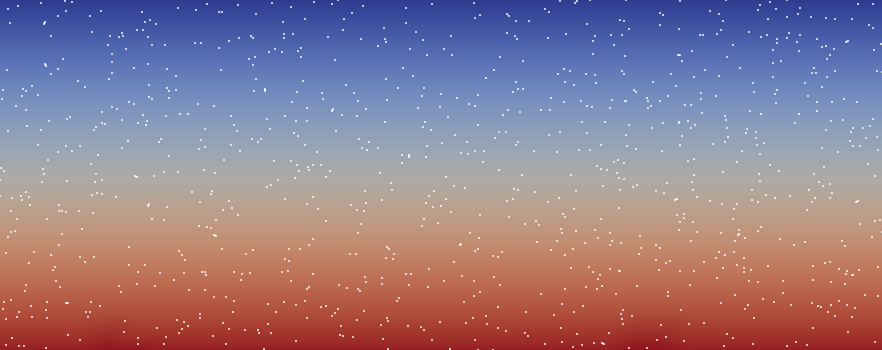
\includegraphics[width=\textwidth]{figures/box_batch0.png}
        \caption{Caption}
        \label{fig:my_label}
    \end{subfigure}
    \hfill
    \begin{subfigure}{0.49\textwidth}
        \centering
        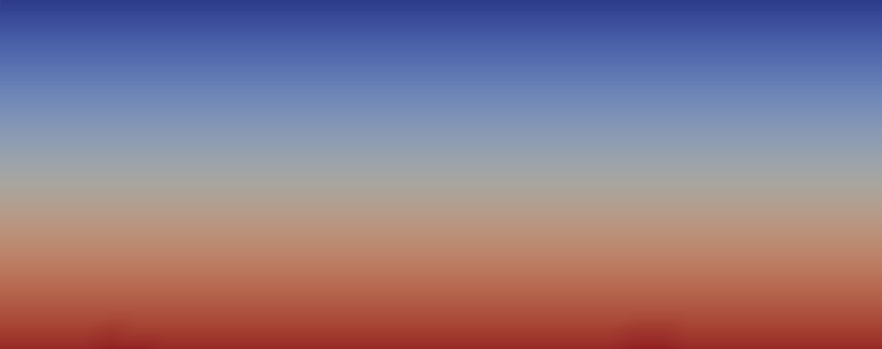
\includegraphics[width=\textwidth]{figures/box_2pp0.png}
        \caption{Caption}
        \label{fig:my_label}
    \end{subfigure}
    %
    \begin{subfigure}{0.49\textwidth}
        \centering
        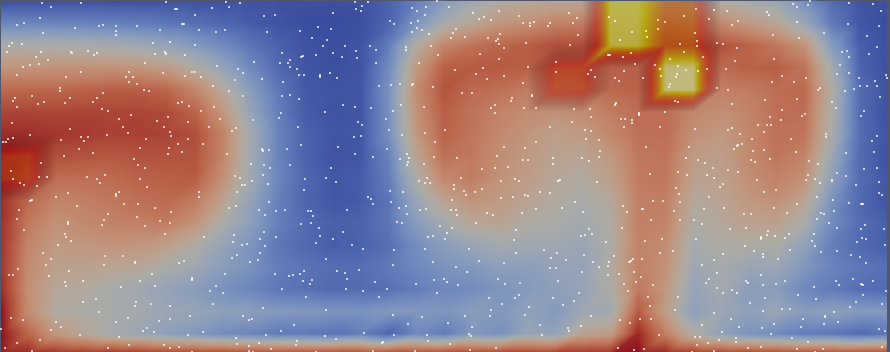
\includegraphics[width=\textwidth]{figures/box_batch38.png}
        \caption{Caption}
        \label{fig:my_label}
    \end{subfigure}
    \hfill
    \begin{subfigure}{0.49\textwidth}
        \centering
        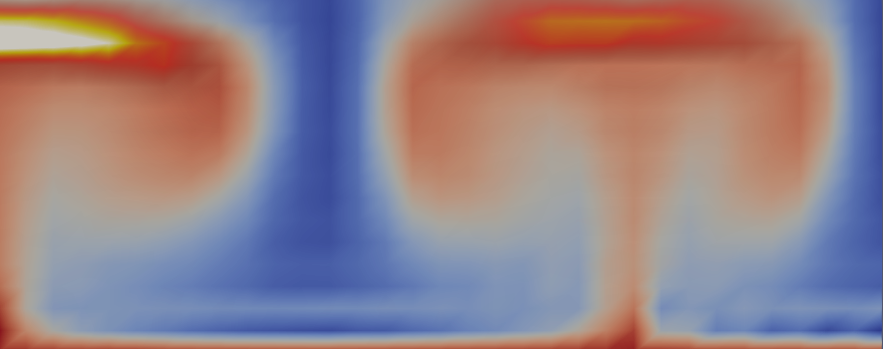
\includegraphics[width=\textwidth]{figures/box_2pp38.png}
        \caption{Caption}
        \label{fig:my_label}
    \end{subfigure}
    %
    \begin{subfigure}{0.49\textwidth}
        \centering
        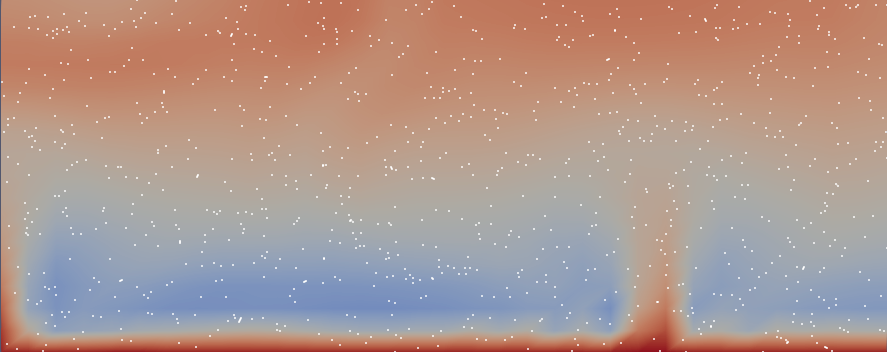
\includegraphics[width=\textwidth]{figures/box_batch79.png}
        \caption{Caption}
        \label{fig:my_label}
    \end{subfigure}
    \hfill
    \begin{subfigure}{0.49\textwidth}
        \centering
        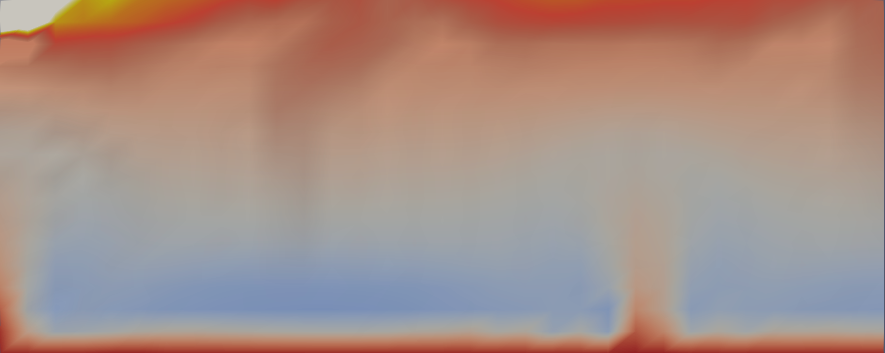
\includegraphics[width=\textwidth]{figures/box_2pp77.png}
        \caption{Caption}
        \label{fig:my_label}
    \end{subfigure}
\end{figure}
\subsection{Decompression event}

\begin{figure}
    \centering
    %% Creator: Matplotlib, PGF backend
%%
%% To include the figure in your LaTeX document, write
%%   \input{<filename>.pgf}
%%
%% Make sure the required packages are loaded in your preamble
%%   \usepackage{pgf}
%%
%% Figures using additional raster images can only be included by \input if
%% they are in the same directory as the main LaTeX file. For loading figures
%% from other directories you can use the `import` package
%%   \usepackage{import}
%% and then include the figures with
%%   \import{<path to file>}{<filename>.pgf}
%%
%% Matplotlib used the following preamble
%%   \usepackage{fontspec}
%%   \setmainfont{DejaVuSerif.ttf}[Path=/home/connor/.local/lib/python3.8/site-packages/matplotlib/mpl-data/fonts/ttf/]
%%   \setsansfont{DejaVuSans.ttf}[Path=/home/connor/.local/lib/python3.8/site-packages/matplotlib/mpl-data/fonts/ttf/]
%%   \setmonofont{DejaVuSansMono.ttf}[Path=/home/connor/.local/lib/python3.8/site-packages/matplotlib/mpl-data/fonts/ttf/]
%%
\begingroup%
\makeatletter%
\begin{pgfpicture}%
\pgfpathrectangle{\pgfpointorigin}{\pgfqpoint{4.004230in}{3.132284in}}%
\pgfusepath{use as bounding box, clip}%
\begin{pgfscope}%
\pgfsetbuttcap%
\pgfsetmiterjoin%
\definecolor{currentfill}{rgb}{1.000000,1.000000,1.000000}%
\pgfsetfillcolor{currentfill}%
\pgfsetlinewidth{0.000000pt}%
\definecolor{currentstroke}{rgb}{1.000000,1.000000,1.000000}%
\pgfsetstrokecolor{currentstroke}%
\pgfsetdash{}{0pt}%
\pgfpathmoveto{\pgfqpoint{0.000000in}{0.000000in}}%
\pgfpathlineto{\pgfqpoint{4.004230in}{0.000000in}}%
\pgfpathlineto{\pgfqpoint{4.004230in}{3.132284in}}%
\pgfpathlineto{\pgfqpoint{0.000000in}{3.132284in}}%
\pgfpathclose%
\pgfusepath{fill}%
\end{pgfscope}%
\begin{pgfscope}%
\pgfsetbuttcap%
\pgfsetmiterjoin%
\definecolor{currentfill}{rgb}{1.000000,1.000000,1.000000}%
\pgfsetfillcolor{currentfill}%
\pgfsetlinewidth{0.000000pt}%
\definecolor{currentstroke}{rgb}{0.000000,0.000000,0.000000}%
\pgfsetstrokecolor{currentstroke}%
\pgfsetstrokeopacity{0.000000}%
\pgfsetdash{}{0pt}%
\pgfpathmoveto{\pgfqpoint{0.511159in}{1.741813in}}%
\pgfpathlineto{\pgfqpoint{3.904230in}{1.741813in}}%
\pgfpathlineto{\pgfqpoint{3.904230in}{3.014215in}}%
\pgfpathlineto{\pgfqpoint{0.511159in}{3.014215in}}%
\pgfpathclose%
\pgfusepath{fill}%
\end{pgfscope}%
\begin{pgfscope}%
\pgfsetbuttcap%
\pgfsetroundjoin%
\definecolor{currentfill}{rgb}{0.000000,0.000000,0.000000}%
\pgfsetfillcolor{currentfill}%
\pgfsetlinewidth{0.803000pt}%
\definecolor{currentstroke}{rgb}{0.000000,0.000000,0.000000}%
\pgfsetstrokecolor{currentstroke}%
\pgfsetdash{}{0pt}%
\pgfsys@defobject{currentmarker}{\pgfqpoint{0.000000in}{-0.048611in}}{\pgfqpoint{0.000000in}{0.000000in}}{%
\pgfpathmoveto{\pgfqpoint{0.000000in}{0.000000in}}%
\pgfpathlineto{\pgfqpoint{0.000000in}{-0.048611in}}%
\pgfusepath{stroke,fill}%
}%
\begin{pgfscope}%
\pgfsys@transformshift{0.665390in}{1.741813in}%
\pgfsys@useobject{currentmarker}{}%
\end{pgfscope}%
\end{pgfscope}%
\begin{pgfscope}%
\definecolor{textcolor}{rgb}{0.000000,0.000000,0.000000}%
\pgfsetstrokecolor{textcolor}%
\pgfsetfillcolor{textcolor}%
\pgftext[x=0.665390in,y=1.644591in,,top]{\color{textcolor}\rmfamily\fontsize{8.000000}{9.600000}\selectfont \(\displaystyle 0\)}%
\end{pgfscope}%
\begin{pgfscope}%
\pgfsetbuttcap%
\pgfsetroundjoin%
\definecolor{currentfill}{rgb}{0.000000,0.000000,0.000000}%
\pgfsetfillcolor{currentfill}%
\pgfsetlinewidth{0.803000pt}%
\definecolor{currentstroke}{rgb}{0.000000,0.000000,0.000000}%
\pgfsetstrokecolor{currentstroke}%
\pgfsetdash{}{0pt}%
\pgfsys@defobject{currentmarker}{\pgfqpoint{0.000000in}{-0.048611in}}{\pgfqpoint{0.000000in}{0.000000in}}{%
\pgfpathmoveto{\pgfqpoint{0.000000in}{0.000000in}}%
\pgfpathlineto{\pgfqpoint{0.000000in}{-0.048611in}}%
\pgfusepath{stroke,fill}%
}%
\begin{pgfscope}%
\pgfsys@transformshift{1.078738in}{1.741813in}%
\pgfsys@useobject{currentmarker}{}%
\end{pgfscope}%
\end{pgfscope}%
\begin{pgfscope}%
\definecolor{textcolor}{rgb}{0.000000,0.000000,0.000000}%
\pgfsetstrokecolor{textcolor}%
\pgfsetfillcolor{textcolor}%
\pgftext[x=1.078738in,y=1.644591in,,top]{\color{textcolor}\rmfamily\fontsize{8.000000}{9.600000}\selectfont \(\displaystyle 20000\)}%
\end{pgfscope}%
\begin{pgfscope}%
\pgfsetbuttcap%
\pgfsetroundjoin%
\definecolor{currentfill}{rgb}{0.000000,0.000000,0.000000}%
\pgfsetfillcolor{currentfill}%
\pgfsetlinewidth{0.803000pt}%
\definecolor{currentstroke}{rgb}{0.000000,0.000000,0.000000}%
\pgfsetstrokecolor{currentstroke}%
\pgfsetdash{}{0pt}%
\pgfsys@defobject{currentmarker}{\pgfqpoint{0.000000in}{-0.048611in}}{\pgfqpoint{0.000000in}{0.000000in}}{%
\pgfpathmoveto{\pgfqpoint{0.000000in}{0.000000in}}%
\pgfpathlineto{\pgfqpoint{0.000000in}{-0.048611in}}%
\pgfusepath{stroke,fill}%
}%
\begin{pgfscope}%
\pgfsys@transformshift{1.492086in}{1.741813in}%
\pgfsys@useobject{currentmarker}{}%
\end{pgfscope}%
\end{pgfscope}%
\begin{pgfscope}%
\definecolor{textcolor}{rgb}{0.000000,0.000000,0.000000}%
\pgfsetstrokecolor{textcolor}%
\pgfsetfillcolor{textcolor}%
\pgftext[x=1.492086in,y=1.644591in,,top]{\color{textcolor}\rmfamily\fontsize{8.000000}{9.600000}\selectfont \(\displaystyle 40000\)}%
\end{pgfscope}%
\begin{pgfscope}%
\pgfsetbuttcap%
\pgfsetroundjoin%
\definecolor{currentfill}{rgb}{0.000000,0.000000,0.000000}%
\pgfsetfillcolor{currentfill}%
\pgfsetlinewidth{0.803000pt}%
\definecolor{currentstroke}{rgb}{0.000000,0.000000,0.000000}%
\pgfsetstrokecolor{currentstroke}%
\pgfsetdash{}{0pt}%
\pgfsys@defobject{currentmarker}{\pgfqpoint{0.000000in}{-0.048611in}}{\pgfqpoint{0.000000in}{0.000000in}}{%
\pgfpathmoveto{\pgfqpoint{0.000000in}{0.000000in}}%
\pgfpathlineto{\pgfqpoint{0.000000in}{-0.048611in}}%
\pgfusepath{stroke,fill}%
}%
\begin{pgfscope}%
\pgfsys@transformshift{1.905434in}{1.741813in}%
\pgfsys@useobject{currentmarker}{}%
\end{pgfscope}%
\end{pgfscope}%
\begin{pgfscope}%
\definecolor{textcolor}{rgb}{0.000000,0.000000,0.000000}%
\pgfsetstrokecolor{textcolor}%
\pgfsetfillcolor{textcolor}%
\pgftext[x=1.905434in,y=1.644591in,,top]{\color{textcolor}\rmfamily\fontsize{8.000000}{9.600000}\selectfont \(\displaystyle 60000\)}%
\end{pgfscope}%
\begin{pgfscope}%
\pgfsetbuttcap%
\pgfsetroundjoin%
\definecolor{currentfill}{rgb}{0.000000,0.000000,0.000000}%
\pgfsetfillcolor{currentfill}%
\pgfsetlinewidth{0.803000pt}%
\definecolor{currentstroke}{rgb}{0.000000,0.000000,0.000000}%
\pgfsetstrokecolor{currentstroke}%
\pgfsetdash{}{0pt}%
\pgfsys@defobject{currentmarker}{\pgfqpoint{0.000000in}{-0.048611in}}{\pgfqpoint{0.000000in}{0.000000in}}{%
\pgfpathmoveto{\pgfqpoint{0.000000in}{0.000000in}}%
\pgfpathlineto{\pgfqpoint{0.000000in}{-0.048611in}}%
\pgfusepath{stroke,fill}%
}%
\begin{pgfscope}%
\pgfsys@transformshift{2.318782in}{1.741813in}%
\pgfsys@useobject{currentmarker}{}%
\end{pgfscope}%
\end{pgfscope}%
\begin{pgfscope}%
\definecolor{textcolor}{rgb}{0.000000,0.000000,0.000000}%
\pgfsetstrokecolor{textcolor}%
\pgfsetfillcolor{textcolor}%
\pgftext[x=2.318782in,y=1.644591in,,top]{\color{textcolor}\rmfamily\fontsize{8.000000}{9.600000}\selectfont \(\displaystyle 80000\)}%
\end{pgfscope}%
\begin{pgfscope}%
\pgfsetbuttcap%
\pgfsetroundjoin%
\definecolor{currentfill}{rgb}{0.000000,0.000000,0.000000}%
\pgfsetfillcolor{currentfill}%
\pgfsetlinewidth{0.803000pt}%
\definecolor{currentstroke}{rgb}{0.000000,0.000000,0.000000}%
\pgfsetstrokecolor{currentstroke}%
\pgfsetdash{}{0pt}%
\pgfsys@defobject{currentmarker}{\pgfqpoint{0.000000in}{-0.048611in}}{\pgfqpoint{0.000000in}{0.000000in}}{%
\pgfpathmoveto{\pgfqpoint{0.000000in}{0.000000in}}%
\pgfpathlineto{\pgfqpoint{0.000000in}{-0.048611in}}%
\pgfusepath{stroke,fill}%
}%
\begin{pgfscope}%
\pgfsys@transformshift{2.732130in}{1.741813in}%
\pgfsys@useobject{currentmarker}{}%
\end{pgfscope}%
\end{pgfscope}%
\begin{pgfscope}%
\definecolor{textcolor}{rgb}{0.000000,0.000000,0.000000}%
\pgfsetstrokecolor{textcolor}%
\pgfsetfillcolor{textcolor}%
\pgftext[x=2.732130in,y=1.644591in,,top]{\color{textcolor}\rmfamily\fontsize{8.000000}{9.600000}\selectfont \(\displaystyle 100000\)}%
\end{pgfscope}%
\begin{pgfscope}%
\pgfsetbuttcap%
\pgfsetroundjoin%
\definecolor{currentfill}{rgb}{0.000000,0.000000,0.000000}%
\pgfsetfillcolor{currentfill}%
\pgfsetlinewidth{0.803000pt}%
\definecolor{currentstroke}{rgb}{0.000000,0.000000,0.000000}%
\pgfsetstrokecolor{currentstroke}%
\pgfsetdash{}{0pt}%
\pgfsys@defobject{currentmarker}{\pgfqpoint{0.000000in}{-0.048611in}}{\pgfqpoint{0.000000in}{0.000000in}}{%
\pgfpathmoveto{\pgfqpoint{0.000000in}{0.000000in}}%
\pgfpathlineto{\pgfqpoint{0.000000in}{-0.048611in}}%
\pgfusepath{stroke,fill}%
}%
\begin{pgfscope}%
\pgfsys@transformshift{3.145478in}{1.741813in}%
\pgfsys@useobject{currentmarker}{}%
\end{pgfscope}%
\end{pgfscope}%
\begin{pgfscope}%
\definecolor{textcolor}{rgb}{0.000000,0.000000,0.000000}%
\pgfsetstrokecolor{textcolor}%
\pgfsetfillcolor{textcolor}%
\pgftext[x=3.145478in,y=1.644591in,,top]{\color{textcolor}\rmfamily\fontsize{8.000000}{9.600000}\selectfont \(\displaystyle 120000\)}%
\end{pgfscope}%
\begin{pgfscope}%
\pgfsetbuttcap%
\pgfsetroundjoin%
\definecolor{currentfill}{rgb}{0.000000,0.000000,0.000000}%
\pgfsetfillcolor{currentfill}%
\pgfsetlinewidth{0.803000pt}%
\definecolor{currentstroke}{rgb}{0.000000,0.000000,0.000000}%
\pgfsetstrokecolor{currentstroke}%
\pgfsetdash{}{0pt}%
\pgfsys@defobject{currentmarker}{\pgfqpoint{0.000000in}{-0.048611in}}{\pgfqpoint{0.000000in}{0.000000in}}{%
\pgfpathmoveto{\pgfqpoint{0.000000in}{0.000000in}}%
\pgfpathlineto{\pgfqpoint{0.000000in}{-0.048611in}}%
\pgfusepath{stroke,fill}%
}%
\begin{pgfscope}%
\pgfsys@transformshift{3.558826in}{1.741813in}%
\pgfsys@useobject{currentmarker}{}%
\end{pgfscope}%
\end{pgfscope}%
\begin{pgfscope}%
\definecolor{textcolor}{rgb}{0.000000,0.000000,0.000000}%
\pgfsetstrokecolor{textcolor}%
\pgfsetfillcolor{textcolor}%
\pgftext[x=3.558826in,y=1.644591in,,top]{\color{textcolor}\rmfamily\fontsize{8.000000}{9.600000}\selectfont \(\displaystyle 140000\)}%
\end{pgfscope}%
\begin{pgfscope}%
\pgfsetbuttcap%
\pgfsetroundjoin%
\definecolor{currentfill}{rgb}{0.000000,0.000000,0.000000}%
\pgfsetfillcolor{currentfill}%
\pgfsetlinewidth{0.803000pt}%
\definecolor{currentstroke}{rgb}{0.000000,0.000000,0.000000}%
\pgfsetstrokecolor{currentstroke}%
\pgfsetdash{}{0pt}%
\pgfsys@defobject{currentmarker}{\pgfqpoint{-0.048611in}{0.000000in}}{\pgfqpoint{0.000000in}{0.000000in}}{%
\pgfpathmoveto{\pgfqpoint{0.000000in}{0.000000in}}%
\pgfpathlineto{\pgfqpoint{-0.048611in}{0.000000in}}%
\pgfusepath{stroke,fill}%
}%
\begin{pgfscope}%
\pgfsys@transformshift{0.511159in}{1.799650in}%
\pgfsys@useobject{currentmarker}{}%
\end{pgfscope}%
\end{pgfscope}%
\begin{pgfscope}%
\definecolor{textcolor}{rgb}{0.000000,0.000000,0.000000}%
\pgfsetstrokecolor{textcolor}%
\pgfsetfillcolor{textcolor}%
\pgftext[x=0.263086in,y=1.757440in,left,base]{\color{textcolor}\rmfamily\fontsize{8.000000}{9.600000}\selectfont \(\displaystyle 0.0\)}%
\end{pgfscope}%
\begin{pgfscope}%
\pgfsetbuttcap%
\pgfsetroundjoin%
\definecolor{currentfill}{rgb}{0.000000,0.000000,0.000000}%
\pgfsetfillcolor{currentfill}%
\pgfsetlinewidth{0.803000pt}%
\definecolor{currentstroke}{rgb}{0.000000,0.000000,0.000000}%
\pgfsetstrokecolor{currentstroke}%
\pgfsetdash{}{0pt}%
\pgfsys@defobject{currentmarker}{\pgfqpoint{-0.048611in}{0.000000in}}{\pgfqpoint{0.000000in}{0.000000in}}{%
\pgfpathmoveto{\pgfqpoint{0.000000in}{0.000000in}}%
\pgfpathlineto{\pgfqpoint{-0.048611in}{0.000000in}}%
\pgfusepath{stroke,fill}%
}%
\begin{pgfscope}%
\pgfsys@transformshift{0.511159in}{2.070813in}%
\pgfsys@useobject{currentmarker}{}%
\end{pgfscope}%
\end{pgfscope}%
\begin{pgfscope}%
\definecolor{textcolor}{rgb}{0.000000,0.000000,0.000000}%
\pgfsetstrokecolor{textcolor}%
\pgfsetfillcolor{textcolor}%
\pgftext[x=0.263086in,y=2.028604in,left,base]{\color{textcolor}\rmfamily\fontsize{8.000000}{9.600000}\selectfont \(\displaystyle 0.5\)}%
\end{pgfscope}%
\begin{pgfscope}%
\pgfsetbuttcap%
\pgfsetroundjoin%
\definecolor{currentfill}{rgb}{0.000000,0.000000,0.000000}%
\pgfsetfillcolor{currentfill}%
\pgfsetlinewidth{0.803000pt}%
\definecolor{currentstroke}{rgb}{0.000000,0.000000,0.000000}%
\pgfsetstrokecolor{currentstroke}%
\pgfsetdash{}{0pt}%
\pgfsys@defobject{currentmarker}{\pgfqpoint{-0.048611in}{0.000000in}}{\pgfqpoint{0.000000in}{0.000000in}}{%
\pgfpathmoveto{\pgfqpoint{0.000000in}{0.000000in}}%
\pgfpathlineto{\pgfqpoint{-0.048611in}{0.000000in}}%
\pgfusepath{stroke,fill}%
}%
\begin{pgfscope}%
\pgfsys@transformshift{0.511159in}{2.341976in}%
\pgfsys@useobject{currentmarker}{}%
\end{pgfscope}%
\end{pgfscope}%
\begin{pgfscope}%
\definecolor{textcolor}{rgb}{0.000000,0.000000,0.000000}%
\pgfsetstrokecolor{textcolor}%
\pgfsetfillcolor{textcolor}%
\pgftext[x=0.263086in,y=2.299767in,left,base]{\color{textcolor}\rmfamily\fontsize{8.000000}{9.600000}\selectfont \(\displaystyle 1.0\)}%
\end{pgfscope}%
\begin{pgfscope}%
\pgfsetbuttcap%
\pgfsetroundjoin%
\definecolor{currentfill}{rgb}{0.000000,0.000000,0.000000}%
\pgfsetfillcolor{currentfill}%
\pgfsetlinewidth{0.803000pt}%
\definecolor{currentstroke}{rgb}{0.000000,0.000000,0.000000}%
\pgfsetstrokecolor{currentstroke}%
\pgfsetdash{}{0pt}%
\pgfsys@defobject{currentmarker}{\pgfqpoint{-0.048611in}{0.000000in}}{\pgfqpoint{0.000000in}{0.000000in}}{%
\pgfpathmoveto{\pgfqpoint{0.000000in}{0.000000in}}%
\pgfpathlineto{\pgfqpoint{-0.048611in}{0.000000in}}%
\pgfusepath{stroke,fill}%
}%
\begin{pgfscope}%
\pgfsys@transformshift{0.511159in}{2.613140in}%
\pgfsys@useobject{currentmarker}{}%
\end{pgfscope}%
\end{pgfscope}%
\begin{pgfscope}%
\definecolor{textcolor}{rgb}{0.000000,0.000000,0.000000}%
\pgfsetstrokecolor{textcolor}%
\pgfsetfillcolor{textcolor}%
\pgftext[x=0.263086in,y=2.570931in,left,base]{\color{textcolor}\rmfamily\fontsize{8.000000}{9.600000}\selectfont \(\displaystyle 1.5\)}%
\end{pgfscope}%
\begin{pgfscope}%
\pgfsetbuttcap%
\pgfsetroundjoin%
\definecolor{currentfill}{rgb}{0.000000,0.000000,0.000000}%
\pgfsetfillcolor{currentfill}%
\pgfsetlinewidth{0.803000pt}%
\definecolor{currentstroke}{rgb}{0.000000,0.000000,0.000000}%
\pgfsetstrokecolor{currentstroke}%
\pgfsetdash{}{0pt}%
\pgfsys@defobject{currentmarker}{\pgfqpoint{-0.048611in}{0.000000in}}{\pgfqpoint{0.000000in}{0.000000in}}{%
\pgfpathmoveto{\pgfqpoint{0.000000in}{0.000000in}}%
\pgfpathlineto{\pgfqpoint{-0.048611in}{0.000000in}}%
\pgfusepath{stroke,fill}%
}%
\begin{pgfscope}%
\pgfsys@transformshift{0.511159in}{2.884303in}%
\pgfsys@useobject{currentmarker}{}%
\end{pgfscope}%
\end{pgfscope}%
\begin{pgfscope}%
\definecolor{textcolor}{rgb}{0.000000,0.000000,0.000000}%
\pgfsetstrokecolor{textcolor}%
\pgfsetfillcolor{textcolor}%
\pgftext[x=0.263086in,y=2.842094in,left,base]{\color{textcolor}\rmfamily\fontsize{8.000000}{9.600000}\selectfont \(\displaystyle 2.0\)}%
\end{pgfscope}%
\begin{pgfscope}%
\definecolor{textcolor}{rgb}{0.000000,0.000000,0.000000}%
\pgfsetstrokecolor{textcolor}%
\pgfsetfillcolor{textcolor}%
\pgftext[x=0.207530in,y=2.378014in,,bottom,rotate=90.000000]{\color{textcolor}\rmfamily\fontsize{8.000000}{9.600000}\selectfont Melt composition (mol)}%
\end{pgfscope}%
\begin{pgfscope}%
\pgfpathrectangle{\pgfqpoint{0.511159in}{1.741813in}}{\pgfqpoint{3.393071in}{1.272402in}}%
\pgfusepath{clip}%
\pgfsetrectcap%
\pgfsetroundjoin%
\pgfsetlinewidth{1.505625pt}%
\definecolor{currentstroke}{rgb}{0.121569,0.466667,0.705882}%
\pgfsetstrokecolor{currentstroke}%
\pgfsetdash{}{0pt}%
\pgfpathmoveto{\pgfqpoint{0.665390in}{1.799650in}}%
\pgfpathlineto{\pgfqpoint{1.393916in}{1.799650in}}%
\pgfpathlineto{\pgfqpoint{1.414583in}{1.825296in}}%
\pgfpathlineto{\pgfqpoint{1.435250in}{2.081757in}}%
\pgfpathlineto{\pgfqpoint{1.497253in}{2.081757in}}%
\pgfpathlineto{\pgfqpoint{1.517920in}{2.093059in}}%
\pgfpathlineto{\pgfqpoint{1.538587in}{2.091644in}}%
\pgfpathlineto{\pgfqpoint{1.559255in}{2.090939in}}%
\pgfpathlineto{\pgfqpoint{1.579922in}{2.081757in}}%
\pgfpathlineto{\pgfqpoint{1.600590in}{2.089529in}}%
\pgfpathlineto{\pgfqpoint{1.641924in}{2.086351in}}%
\pgfpathlineto{\pgfqpoint{1.662592in}{2.070461in}}%
\pgfpathlineto{\pgfqpoint{1.765929in}{2.070461in}}%
\pgfpathlineto{\pgfqpoint{1.786596in}{2.064810in}}%
\pgfpathlineto{\pgfqpoint{1.807264in}{2.070461in}}%
\pgfpathlineto{\pgfqpoint{1.848598in}{2.070461in}}%
\pgfpathlineto{\pgfqpoint{1.869266in}{2.068308in}}%
\pgfpathlineto{\pgfqpoint{1.889933in}{2.068340in}}%
\pgfpathlineto{\pgfqpoint{1.910601in}{2.064115in}}%
\pgfpathlineto{\pgfqpoint{1.931268in}{2.062808in}}%
\pgfpathlineto{\pgfqpoint{1.951935in}{2.059869in}}%
\pgfpathlineto{\pgfqpoint{1.972603in}{2.059869in}}%
\pgfpathlineto{\pgfqpoint{1.993270in}{2.057396in}}%
\pgfpathlineto{\pgfqpoint{2.075940in}{2.050687in}}%
\pgfpathlineto{\pgfqpoint{2.096607in}{2.047862in}}%
\pgfpathlineto{\pgfqpoint{2.117275in}{2.047412in}}%
\pgfpathlineto{\pgfqpoint{2.158609in}{2.042759in}}%
\pgfpathlineto{\pgfqpoint{2.179277in}{2.041506in}}%
\pgfpathlineto{\pgfqpoint{2.261946in}{2.030209in}}%
\pgfpathlineto{\pgfqpoint{2.282614in}{2.028799in}}%
\pgfpathlineto{\pgfqpoint{2.303281in}{2.026679in}}%
\pgfpathlineto{\pgfqpoint{2.323949in}{2.025572in}}%
\pgfpathlineto{\pgfqpoint{2.344616in}{2.023853in}}%
\pgfpathlineto{\pgfqpoint{2.406618in}{2.016087in}}%
\pgfpathlineto{\pgfqpoint{2.427286in}{2.014319in}}%
\pgfpathlineto{\pgfqpoint{2.489288in}{2.004215in}}%
\pgfpathlineto{\pgfqpoint{2.509955in}{2.003375in}}%
\pgfpathlineto{\pgfqpoint{2.551290in}{2.003375in}}%
\pgfpathlineto{\pgfqpoint{2.571958in}{1.997724in}}%
\pgfpathlineto{\pgfqpoint{2.592625in}{1.995961in}}%
\pgfpathlineto{\pgfqpoint{2.654627in}{1.986731in}}%
\pgfpathlineto{\pgfqpoint{2.675295in}{1.985245in}}%
\pgfpathlineto{\pgfqpoint{2.695962in}{1.982191in}}%
\pgfpathlineto{\pgfqpoint{2.716629in}{1.982099in}}%
\pgfpathlineto{\pgfqpoint{2.737297in}{1.983075in}}%
\pgfpathlineto{\pgfqpoint{2.757964in}{1.982186in}}%
\pgfpathlineto{\pgfqpoint{3.005973in}{1.982962in}}%
\pgfpathlineto{\pgfqpoint{3.150645in}{1.982897in}}%
\pgfpathlineto{\pgfqpoint{3.274649in}{1.983200in}}%
\pgfpathlineto{\pgfqpoint{3.315984in}{1.982897in}}%
\pgfpathlineto{\pgfqpoint{3.481323in}{1.982436in}}%
\pgfpathlineto{\pgfqpoint{3.605328in}{1.981774in}}%
\pgfpathlineto{\pgfqpoint{3.646662in}{1.982392in}}%
\pgfpathlineto{\pgfqpoint{3.667330in}{1.981503in}}%
\pgfpathlineto{\pgfqpoint{3.687997in}{1.981644in}}%
\pgfpathlineto{\pgfqpoint{3.708665in}{1.982436in}}%
\pgfpathlineto{\pgfqpoint{3.729332in}{1.981091in}}%
\pgfpathlineto{\pgfqpoint{3.750000in}{1.981053in}}%
\pgfpathlineto{\pgfqpoint{3.750000in}{1.981053in}}%
\pgfusepath{stroke}%
\end{pgfscope}%
\begin{pgfscope}%
\pgfpathrectangle{\pgfqpoint{0.511159in}{1.741813in}}{\pgfqpoint{3.393071in}{1.272402in}}%
\pgfusepath{clip}%
\pgfsetrectcap%
\pgfsetroundjoin%
\pgfsetlinewidth{1.505625pt}%
\definecolor{currentstroke}{rgb}{1.000000,0.498039,0.054902}%
\pgfsetstrokecolor{currentstroke}%
\pgfsetdash{}{0pt}%
\pgfpathmoveto{\pgfqpoint{0.665390in}{1.799650in}}%
\pgfpathlineto{\pgfqpoint{1.393916in}{1.799650in}}%
\pgfpathlineto{\pgfqpoint{1.414583in}{1.821605in}}%
\pgfpathlineto{\pgfqpoint{1.435250in}{2.039743in}}%
\pgfpathlineto{\pgfqpoint{1.455918in}{2.036918in}}%
\pgfpathlineto{\pgfqpoint{1.476585in}{2.032682in}}%
\pgfpathlineto{\pgfqpoint{1.497253in}{2.031267in}}%
\pgfpathlineto{\pgfqpoint{1.517920in}{2.024206in}}%
\pgfpathlineto{\pgfqpoint{1.538587in}{2.022795in}}%
\pgfpathlineto{\pgfqpoint{1.559255in}{2.022795in}}%
\pgfpathlineto{\pgfqpoint{1.579922in}{2.024206in}}%
\pgfpathlineto{\pgfqpoint{1.600590in}{2.021380in}}%
\pgfpathlineto{\pgfqpoint{1.641924in}{2.018560in}}%
\pgfpathlineto{\pgfqpoint{1.662592in}{2.021380in}}%
\pgfpathlineto{\pgfqpoint{1.724594in}{2.017144in}}%
\pgfpathlineto{\pgfqpoint{1.745261in}{2.014319in}}%
\pgfpathlineto{\pgfqpoint{1.786596in}{2.014319in}}%
\pgfpathlineto{\pgfqpoint{1.807264in}{2.011493in}}%
\pgfpathlineto{\pgfqpoint{1.848598in}{2.011493in}}%
\pgfpathlineto{\pgfqpoint{1.869266in}{2.008798in}}%
\pgfpathlineto{\pgfqpoint{1.889933in}{2.003022in}}%
\pgfpathlineto{\pgfqpoint{1.910601in}{2.011266in}}%
\pgfpathlineto{\pgfqpoint{1.931268in}{2.010083in}}%
\pgfpathlineto{\pgfqpoint{1.951935in}{2.010083in}}%
\pgfpathlineto{\pgfqpoint{1.972603in}{2.004432in}}%
\pgfpathlineto{\pgfqpoint{1.993270in}{2.004432in}}%
\pgfpathlineto{\pgfqpoint{2.013938in}{2.003022in}}%
\pgfpathlineto{\pgfqpoint{2.034605in}{2.003022in}}%
\pgfpathlineto{\pgfqpoint{2.055272in}{2.001612in}}%
\pgfpathlineto{\pgfqpoint{2.096607in}{2.001612in}}%
\pgfpathlineto{\pgfqpoint{2.137942in}{1.998787in}}%
\pgfpathlineto{\pgfqpoint{2.158609in}{1.998787in}}%
\pgfpathlineto{\pgfqpoint{2.179277in}{1.997707in}}%
\pgfpathlineto{\pgfqpoint{2.199944in}{1.997371in}}%
\pgfpathlineto{\pgfqpoint{2.261946in}{1.993136in}}%
\pgfpathlineto{\pgfqpoint{2.323949in}{1.992935in}}%
\pgfpathlineto{\pgfqpoint{2.365283in}{1.991026in}}%
\pgfpathlineto{\pgfqpoint{2.385951in}{1.990310in}}%
\pgfpathlineto{\pgfqpoint{2.406618in}{1.990310in}}%
\pgfpathlineto{\pgfqpoint{2.447953in}{1.988900in}}%
\pgfpathlineto{\pgfqpoint{2.489288in}{1.986617in}}%
\pgfpathlineto{\pgfqpoint{2.530623in}{1.984795in}}%
\pgfpathlineto{\pgfqpoint{2.571958in}{1.984220in}}%
\pgfpathlineto{\pgfqpoint{2.654627in}{1.980424in}}%
\pgfpathlineto{\pgfqpoint{2.675295in}{1.980277in}}%
\pgfpathlineto{\pgfqpoint{2.695962in}{1.979013in}}%
\pgfpathlineto{\pgfqpoint{2.737297in}{1.979333in}}%
\pgfpathlineto{\pgfqpoint{2.778632in}{1.981123in}}%
\pgfpathlineto{\pgfqpoint{2.819966in}{1.981150in}}%
\pgfpathlineto{\pgfqpoint{2.881969in}{1.983038in}}%
\pgfpathlineto{\pgfqpoint{2.943971in}{1.983249in}}%
\pgfpathlineto{\pgfqpoint{2.964638in}{1.984664in}}%
\pgfpathlineto{\pgfqpoint{3.005973in}{1.984968in}}%
\pgfpathlineto{\pgfqpoint{3.047308in}{1.986834in}}%
\pgfpathlineto{\pgfqpoint{3.067975in}{1.986839in}}%
\pgfpathlineto{\pgfqpoint{3.088643in}{1.987485in}}%
\pgfpathlineto{\pgfqpoint{3.109310in}{1.987485in}}%
\pgfpathlineto{\pgfqpoint{3.129977in}{1.988705in}}%
\pgfpathlineto{\pgfqpoint{3.171312in}{1.988900in}}%
\pgfpathlineto{\pgfqpoint{3.191980in}{1.990261in}}%
\pgfpathlineto{\pgfqpoint{3.233314in}{1.990310in}}%
\pgfpathlineto{\pgfqpoint{3.253982in}{1.991726in}}%
\pgfpathlineto{\pgfqpoint{3.274649in}{1.992105in}}%
\pgfpathlineto{\pgfqpoint{3.295317in}{1.993136in}}%
\pgfpathlineto{\pgfqpoint{3.315984in}{1.993136in}}%
\pgfpathlineto{\pgfqpoint{3.357319in}{1.994204in}}%
\pgfpathlineto{\pgfqpoint{3.439988in}{1.995961in}}%
\pgfpathlineto{\pgfqpoint{3.460656in}{1.997371in}}%
\pgfpathlineto{\pgfqpoint{3.501991in}{1.997458in}}%
\pgfpathlineto{\pgfqpoint{3.522658in}{1.999221in}}%
\pgfpathlineto{\pgfqpoint{3.563993in}{2.000728in}}%
\pgfpathlineto{\pgfqpoint{3.584660in}{2.000929in}}%
\pgfpathlineto{\pgfqpoint{3.605328in}{2.000197in}}%
\pgfpathlineto{\pgfqpoint{3.646662in}{1.997496in}}%
\pgfpathlineto{\pgfqpoint{3.667330in}{2.000929in}}%
\pgfpathlineto{\pgfqpoint{3.687997in}{2.002811in}}%
\pgfpathlineto{\pgfqpoint{3.708665in}{2.001612in}}%
\pgfpathlineto{\pgfqpoint{3.729332in}{2.002632in}}%
\pgfpathlineto{\pgfqpoint{3.750000in}{2.002616in}}%
\pgfpathlineto{\pgfqpoint{3.750000in}{2.002616in}}%
\pgfusepath{stroke}%
\end{pgfscope}%
\begin{pgfscope}%
\pgfpathrectangle{\pgfqpoint{0.511159in}{1.741813in}}{\pgfqpoint{3.393071in}{1.272402in}}%
\pgfusepath{clip}%
\pgfsetrectcap%
\pgfsetroundjoin%
\pgfsetlinewidth{1.505625pt}%
\definecolor{currentstroke}{rgb}{0.172549,0.627451,0.172549}%
\pgfsetstrokecolor{currentstroke}%
\pgfsetdash{}{0pt}%
\pgfpathmoveto{\pgfqpoint{0.665390in}{1.799650in}}%
\pgfpathlineto{\pgfqpoint{1.393916in}{1.799650in}}%
\pgfpathlineto{\pgfqpoint{1.414583in}{1.860379in}}%
\pgfpathlineto{\pgfqpoint{1.435250in}{2.467688in}}%
\pgfpathlineto{\pgfqpoint{1.476585in}{2.467688in}}%
\pgfpathlineto{\pgfqpoint{1.497253in}{2.466278in}}%
\pgfpathlineto{\pgfqpoint{1.517920in}{2.440843in}}%
\pgfpathlineto{\pgfqpoint{1.538587in}{2.443663in}}%
\pgfpathlineto{\pgfqpoint{1.559255in}{2.443663in}}%
\pgfpathlineto{\pgfqpoint{1.579922in}{2.464868in}}%
\pgfpathlineto{\pgfqpoint{1.600590in}{2.446483in}}%
\pgfpathlineto{\pgfqpoint{1.641924in}{2.452123in}}%
\pgfpathlineto{\pgfqpoint{1.662592in}{2.486018in}}%
\pgfpathlineto{\pgfqpoint{1.683259in}{2.486018in}}%
\pgfpathlineto{\pgfqpoint{1.703927in}{2.484608in}}%
\pgfpathlineto{\pgfqpoint{1.724594in}{2.481788in}}%
\pgfpathlineto{\pgfqpoint{1.745261in}{2.481788in}}%
\pgfpathlineto{\pgfqpoint{1.765929in}{2.478968in}}%
\pgfpathlineto{\pgfqpoint{1.786596in}{2.490249in}}%
\pgfpathlineto{\pgfqpoint{1.807264in}{2.476148in}}%
\pgfpathlineto{\pgfqpoint{1.827931in}{2.476148in}}%
\pgfpathlineto{\pgfqpoint{1.848598in}{2.473328in}}%
\pgfpathlineto{\pgfqpoint{1.869266in}{2.476148in}}%
\pgfpathlineto{\pgfqpoint{1.889933in}{2.477558in}}%
\pgfpathlineto{\pgfqpoint{1.910601in}{2.480378in}}%
\pgfpathlineto{\pgfqpoint{1.931268in}{2.481788in}}%
\pgfpathlineto{\pgfqpoint{1.951935in}{2.484608in}}%
\pgfpathlineto{\pgfqpoint{1.972603in}{2.486018in}}%
\pgfpathlineto{\pgfqpoint{2.034605in}{2.494479in}}%
\pgfpathlineto{\pgfqpoint{2.075940in}{2.497353in}}%
\pgfpathlineto{\pgfqpoint{2.096607in}{2.501583in}}%
\pgfpathlineto{\pgfqpoint{2.117275in}{2.500173in}}%
\pgfpathlineto{\pgfqpoint{2.137942in}{2.502993in}}%
\pgfpathlineto{\pgfqpoint{2.199944in}{2.508633in}}%
\pgfpathlineto{\pgfqpoint{2.220612in}{2.512864in}}%
\pgfpathlineto{\pgfqpoint{2.261946in}{2.518504in}}%
\pgfpathlineto{\pgfqpoint{2.282614in}{2.518504in}}%
\pgfpathlineto{\pgfqpoint{2.303281in}{2.521324in}}%
\pgfpathlineto{\pgfqpoint{2.323949in}{2.521541in}}%
\pgfpathlineto{\pgfqpoint{2.344616in}{2.522734in}}%
\pgfpathlineto{\pgfqpoint{2.385951in}{2.528428in}}%
\pgfpathlineto{\pgfqpoint{2.427286in}{2.531249in}}%
\pgfpathlineto{\pgfqpoint{2.489288in}{2.539166in}}%
\pgfpathlineto{\pgfqpoint{2.509955in}{2.537431in}}%
\pgfpathlineto{\pgfqpoint{2.530623in}{2.534448in}}%
\pgfpathlineto{\pgfqpoint{2.551290in}{2.532659in}}%
\pgfpathlineto{\pgfqpoint{2.571958in}{2.542963in}}%
\pgfpathlineto{\pgfqpoint{2.592625in}{2.545349in}}%
\pgfpathlineto{\pgfqpoint{2.633960in}{2.548169in}}%
\pgfpathlineto{\pgfqpoint{2.654627in}{2.550447in}}%
\pgfpathlineto{\pgfqpoint{2.675295in}{2.550989in}}%
\pgfpathlineto{\pgfqpoint{2.695962in}{2.552399in}}%
\pgfpathlineto{\pgfqpoint{2.716629in}{2.551369in}}%
\pgfpathlineto{\pgfqpoint{2.737297in}{2.544536in}}%
\pgfpathlineto{\pgfqpoint{2.757964in}{2.549579in}}%
\pgfpathlineto{\pgfqpoint{2.799299in}{2.546759in}}%
\pgfpathlineto{\pgfqpoint{2.819966in}{2.546759in}}%
\pgfpathlineto{\pgfqpoint{2.840634in}{2.545349in}}%
\pgfpathlineto{\pgfqpoint{2.861301in}{2.545349in}}%
\pgfpathlineto{\pgfqpoint{2.881969in}{2.543939in}}%
\pgfpathlineto{\pgfqpoint{2.902636in}{2.543939in}}%
\pgfpathlineto{\pgfqpoint{2.923303in}{2.542529in}}%
\pgfpathlineto{\pgfqpoint{2.943971in}{2.542529in}}%
\pgfpathlineto{\pgfqpoint{2.964638in}{2.541119in}}%
\pgfpathlineto{\pgfqpoint{2.985306in}{2.541119in}}%
\pgfpathlineto{\pgfqpoint{3.005973in}{2.539709in}}%
\pgfpathlineto{\pgfqpoint{3.047308in}{2.538299in}}%
\pgfpathlineto{\pgfqpoint{3.067975in}{2.538245in}}%
\pgfpathlineto{\pgfqpoint{3.088643in}{2.536889in}}%
\pgfpathlineto{\pgfqpoint{3.150645in}{2.536401in}}%
\pgfpathlineto{\pgfqpoint{3.171312in}{2.535479in}}%
\pgfpathlineto{\pgfqpoint{3.212647in}{2.535316in}}%
\pgfpathlineto{\pgfqpoint{3.233314in}{2.534069in}}%
\pgfpathlineto{\pgfqpoint{3.274649in}{2.534069in}}%
\pgfpathlineto{\pgfqpoint{3.295317in}{2.535099in}}%
\pgfpathlineto{\pgfqpoint{3.315984in}{2.535099in}}%
\pgfpathlineto{\pgfqpoint{3.357319in}{2.534069in}}%
\pgfpathlineto{\pgfqpoint{3.481323in}{2.534069in}}%
\pgfpathlineto{\pgfqpoint{3.501991in}{2.535208in}}%
\pgfpathlineto{\pgfqpoint{3.543325in}{2.535479in}}%
\pgfpathlineto{\pgfqpoint{3.563993in}{2.536889in}}%
\pgfpathlineto{\pgfqpoint{3.584660in}{2.536889in}}%
\pgfpathlineto{\pgfqpoint{3.625995in}{2.534286in}}%
\pgfpathlineto{\pgfqpoint{3.646662in}{2.534231in}}%
\pgfpathlineto{\pgfqpoint{3.667330in}{2.536889in}}%
\pgfpathlineto{\pgfqpoint{3.687997in}{2.534069in}}%
\pgfpathlineto{\pgfqpoint{3.708665in}{2.529838in}}%
\pgfpathlineto{\pgfqpoint{3.729332in}{2.538028in}}%
\pgfpathlineto{\pgfqpoint{3.750000in}{2.538299in}}%
\pgfpathlineto{\pgfqpoint{3.750000in}{2.538299in}}%
\pgfusepath{stroke}%
\end{pgfscope}%
\begin{pgfscope}%
\pgfpathrectangle{\pgfqpoint{0.511159in}{1.741813in}}{\pgfqpoint{3.393071in}{1.272402in}}%
\pgfusepath{clip}%
\pgfsetrectcap%
\pgfsetroundjoin%
\pgfsetlinewidth{1.505625pt}%
\definecolor{currentstroke}{rgb}{0.839216,0.152941,0.156863}%
\pgfsetstrokecolor{currentstroke}%
\pgfsetdash{}{0pt}%
\pgfpathmoveto{\pgfqpoint{0.665390in}{1.799650in}}%
\pgfpathlineto{\pgfqpoint{1.393916in}{1.799650in}}%
\pgfpathlineto{\pgfqpoint{1.414583in}{1.878580in}}%
\pgfpathlineto{\pgfqpoint{1.435250in}{2.668566in}}%
\pgfpathlineto{\pgfqpoint{1.455918in}{2.669976in}}%
\pgfpathlineto{\pgfqpoint{1.476585in}{2.672091in}}%
\pgfpathlineto{\pgfqpoint{1.497253in}{2.673501in}}%
\pgfpathlineto{\pgfqpoint{1.517920in}{2.655875in}}%
\pgfpathlineto{\pgfqpoint{1.538587in}{2.659400in}}%
\pgfpathlineto{\pgfqpoint{1.559255in}{2.661515in}}%
\pgfpathlineto{\pgfqpoint{1.579922in}{2.677731in}}%
\pgfpathlineto{\pgfqpoint{1.600590in}{2.665041in}}%
\pgfpathlineto{\pgfqpoint{1.621257in}{2.669650in}}%
\pgfpathlineto{\pgfqpoint{1.641924in}{2.673175in}}%
\pgfpathlineto{\pgfqpoint{1.662592in}{2.702461in}}%
\pgfpathlineto{\pgfqpoint{1.683259in}{2.703166in}}%
\pgfpathlineto{\pgfqpoint{1.703927in}{2.704576in}}%
\pgfpathlineto{\pgfqpoint{1.724594in}{2.706691in}}%
\pgfpathlineto{\pgfqpoint{1.765929in}{2.709511in}}%
\pgfpathlineto{\pgfqpoint{1.786596in}{2.720846in}}%
\pgfpathlineto{\pgfqpoint{1.807264in}{2.712331in}}%
\pgfpathlineto{\pgfqpoint{1.827931in}{2.712331in}}%
\pgfpathlineto{\pgfqpoint{1.848598in}{2.713741in}}%
\pgfpathlineto{\pgfqpoint{1.869266in}{2.720141in}}%
\pgfpathlineto{\pgfqpoint{1.889933in}{2.722256in}}%
\pgfpathlineto{\pgfqpoint{1.910601in}{2.729415in}}%
\pgfpathlineto{\pgfqpoint{1.931268in}{2.733211in}}%
\pgfpathlineto{\pgfqpoint{1.951935in}{2.740587in}}%
\pgfpathlineto{\pgfqpoint{1.972603in}{2.742702in}}%
\pgfpathlineto{\pgfqpoint{1.993270in}{2.748722in}}%
\pgfpathlineto{\pgfqpoint{2.055272in}{2.762497in}}%
\pgfpathlineto{\pgfqpoint{2.075940in}{2.766022in}}%
\pgfpathlineto{\pgfqpoint{2.096607in}{2.772367in}}%
\pgfpathlineto{\pgfqpoint{2.117275in}{2.775133in}}%
\pgfpathlineto{\pgfqpoint{2.158609in}{2.787389in}}%
\pgfpathlineto{\pgfqpoint{2.179277in}{2.790752in}}%
\pgfpathlineto{\pgfqpoint{2.199944in}{2.798507in}}%
\pgfpathlineto{\pgfqpoint{2.220612in}{2.807022in}}%
\pgfpathlineto{\pgfqpoint{2.241279in}{2.813313in}}%
\pgfpathlineto{\pgfqpoint{2.261946in}{2.821122in}}%
\pgfpathlineto{\pgfqpoint{2.282614in}{2.825352in}}%
\pgfpathlineto{\pgfqpoint{2.303281in}{2.830287in}}%
\pgfpathlineto{\pgfqpoint{2.323949in}{2.833596in}}%
\pgfpathlineto{\pgfqpoint{2.344616in}{2.838748in}}%
\pgfpathlineto{\pgfqpoint{2.365283in}{2.845418in}}%
\pgfpathlineto{\pgfqpoint{2.385951in}{2.853282in}}%
\pgfpathlineto{\pgfqpoint{2.406618in}{2.859248in}}%
\pgfpathlineto{\pgfqpoint{2.427286in}{2.864183in}}%
\pgfpathlineto{\pgfqpoint{2.468620in}{2.883436in}}%
\pgfpathlineto{\pgfqpoint{2.489288in}{2.892004in}}%
\pgfpathlineto{\pgfqpoint{2.509955in}{2.895963in}}%
\pgfpathlineto{\pgfqpoint{2.530623in}{2.897807in}}%
\pgfpathlineto{\pgfqpoint{2.551290in}{2.898783in}}%
\pgfpathlineto{\pgfqpoint{2.571958in}{2.910769in}}%
\pgfpathlineto{\pgfqpoint{2.592625in}{2.915379in}}%
\pgfpathlineto{\pgfqpoint{2.613292in}{2.924924in}}%
\pgfpathlineto{\pgfqpoint{2.654627in}{2.941898in}}%
\pgfpathlineto{\pgfqpoint{2.675295in}{2.946183in}}%
\pgfpathlineto{\pgfqpoint{2.695962in}{2.955294in}}%
\pgfpathlineto{\pgfqpoint{2.737297in}{2.956378in}}%
\pgfpathlineto{\pgfqpoint{2.778632in}{2.956053in}}%
\pgfpathlineto{\pgfqpoint{3.109310in}{2.956378in}}%
\pgfpathlineto{\pgfqpoint{3.171312in}{2.956378in}}%
\pgfpathlineto{\pgfqpoint{3.191980in}{2.954968in}}%
\pgfpathlineto{\pgfqpoint{3.605328in}{2.954263in}}%
\pgfpathlineto{\pgfqpoint{3.646662in}{2.954535in}}%
\pgfpathlineto{\pgfqpoint{3.687997in}{2.954209in}}%
\pgfpathlineto{\pgfqpoint{3.708665in}{2.954535in}}%
\pgfpathlineto{\pgfqpoint{3.729332in}{2.953938in}}%
\pgfpathlineto{\pgfqpoint{3.750000in}{2.953938in}}%
\pgfpathlineto{\pgfqpoint{3.750000in}{2.953938in}}%
\pgfusepath{stroke}%
\end{pgfscope}%
\begin{pgfscope}%
\pgfsetrectcap%
\pgfsetmiterjoin%
\pgfsetlinewidth{0.803000pt}%
\definecolor{currentstroke}{rgb}{0.000000,0.000000,0.000000}%
\pgfsetstrokecolor{currentstroke}%
\pgfsetdash{}{0pt}%
\pgfpathmoveto{\pgfqpoint{0.511159in}{1.741813in}}%
\pgfpathlineto{\pgfqpoint{0.511159in}{3.014215in}}%
\pgfusepath{stroke}%
\end{pgfscope}%
\begin{pgfscope}%
\pgfsetrectcap%
\pgfsetmiterjoin%
\pgfsetlinewidth{0.803000pt}%
\definecolor{currentstroke}{rgb}{0.000000,0.000000,0.000000}%
\pgfsetstrokecolor{currentstroke}%
\pgfsetdash{}{0pt}%
\pgfpathmoveto{\pgfqpoint{3.904230in}{1.741813in}}%
\pgfpathlineto{\pgfqpoint{3.904230in}{3.014215in}}%
\pgfusepath{stroke}%
\end{pgfscope}%
\begin{pgfscope}%
\pgfsetrectcap%
\pgfsetmiterjoin%
\pgfsetlinewidth{0.803000pt}%
\definecolor{currentstroke}{rgb}{0.000000,0.000000,0.000000}%
\pgfsetstrokecolor{currentstroke}%
\pgfsetdash{}{0pt}%
\pgfpathmoveto{\pgfqpoint{0.511159in}{1.741813in}}%
\pgfpathlineto{\pgfqpoint{3.904230in}{1.741813in}}%
\pgfusepath{stroke}%
\end{pgfscope}%
\begin{pgfscope}%
\pgfsetrectcap%
\pgfsetmiterjoin%
\pgfsetlinewidth{0.803000pt}%
\definecolor{currentstroke}{rgb}{0.000000,0.000000,0.000000}%
\pgfsetstrokecolor{currentstroke}%
\pgfsetdash{}{0pt}%
\pgfpathmoveto{\pgfqpoint{0.511159in}{3.014215in}}%
\pgfpathlineto{\pgfqpoint{3.904230in}{3.014215in}}%
\pgfusepath{stroke}%
\end{pgfscope}%
\begin{pgfscope}%
\pgfsetrectcap%
\pgfsetroundjoin%
\pgfsetlinewidth{1.505625pt}%
\definecolor{currentstroke}{rgb}{0.121569,0.466667,0.705882}%
\pgfsetstrokecolor{currentstroke}%
\pgfsetdash{}{0pt}%
\pgfpathmoveto{\pgfqpoint{0.611159in}{2.868685in}}%
\pgfpathlineto{\pgfqpoint{0.833381in}{2.868685in}}%
\pgfusepath{stroke}%
\end{pgfscope}%
\begin{pgfscope}%
\definecolor{textcolor}{rgb}{0.000000,0.000000,0.000000}%
\pgfsetstrokecolor{textcolor}%
\pgfsetfillcolor{textcolor}%
\pgftext[x=0.922270in,y=2.829796in,left,base]{\color{textcolor}\rmfamily\fontsize{8.000000}{9.600000}\selectfont CaO}%
\end{pgfscope}%
\begin{pgfscope}%
\pgfsetrectcap%
\pgfsetroundjoin%
\pgfsetlinewidth{1.505625pt}%
\definecolor{currentstroke}{rgb}{1.000000,0.498039,0.054902}%
\pgfsetstrokecolor{currentstroke}%
\pgfsetdash{}{0pt}%
\pgfpathmoveto{\pgfqpoint{0.611159in}{2.705599in}}%
\pgfpathlineto{\pgfqpoint{0.833381in}{2.705599in}}%
\pgfusepath{stroke}%
\end{pgfscope}%
\begin{pgfscope}%
\definecolor{textcolor}{rgb}{0.000000,0.000000,0.000000}%
\pgfsetstrokecolor{textcolor}%
\pgfsetfillcolor{textcolor}%
\pgftext[x=0.922270in,y=2.666711in,left,base]{\color{textcolor}\rmfamily\fontsize{8.000000}{9.600000}\selectfont FeO}%
\end{pgfscope}%
\begin{pgfscope}%
\pgfsetrectcap%
\pgfsetroundjoin%
\pgfsetlinewidth{1.505625pt}%
\definecolor{currentstroke}{rgb}{0.172549,0.627451,0.172549}%
\pgfsetstrokecolor{currentstroke}%
\pgfsetdash{}{0pt}%
\pgfpathmoveto{\pgfqpoint{0.611159in}{2.542514in}}%
\pgfpathlineto{\pgfqpoint{0.833381in}{2.542514in}}%
\pgfusepath{stroke}%
\end{pgfscope}%
\begin{pgfscope}%
\definecolor{textcolor}{rgb}{0.000000,0.000000,0.000000}%
\pgfsetstrokecolor{textcolor}%
\pgfsetfillcolor{textcolor}%
\pgftext[x=0.922270in,y=2.503625in,left,base]{\color{textcolor}\rmfamily\fontsize{8.000000}{9.600000}\selectfont MgO}%
\end{pgfscope}%
\begin{pgfscope}%
\pgfsetrectcap%
\pgfsetroundjoin%
\pgfsetlinewidth{1.505625pt}%
\definecolor{currentstroke}{rgb}{0.839216,0.152941,0.156863}%
\pgfsetstrokecolor{currentstroke}%
\pgfsetdash{}{0pt}%
\pgfpathmoveto{\pgfqpoint{0.611159in}{2.377854in}}%
\pgfpathlineto{\pgfqpoint{0.833381in}{2.377854in}}%
\pgfusepath{stroke}%
\end{pgfscope}%
\begin{pgfscope}%
\definecolor{textcolor}{rgb}{0.000000,0.000000,0.000000}%
\pgfsetstrokecolor{textcolor}%
\pgfsetfillcolor{textcolor}%
\pgftext[x=0.922270in,y=2.338966in,left,base]{\color{textcolor}\rmfamily\fontsize{8.000000}{9.600000}\selectfont SiO2}%
\end{pgfscope}%
\begin{pgfscope}%
\pgfsetbuttcap%
\pgfsetmiterjoin%
\definecolor{currentfill}{rgb}{1.000000,1.000000,1.000000}%
\pgfsetfillcolor{currentfill}%
\pgfsetlinewidth{0.000000pt}%
\definecolor{currentstroke}{rgb}{0.000000,0.000000,0.000000}%
\pgfsetstrokecolor{currentstroke}%
\pgfsetstrokeopacity{0.000000}%
\pgfsetdash{}{0pt}%
\pgfpathmoveto{\pgfqpoint{0.511159in}{0.469412in}}%
\pgfpathlineto{\pgfqpoint{3.904230in}{0.469412in}}%
\pgfpathlineto{\pgfqpoint{3.904230in}{1.423713in}}%
\pgfpathlineto{\pgfqpoint{0.511159in}{1.423713in}}%
\pgfpathclose%
\pgfusepath{fill}%
\end{pgfscope}%
\begin{pgfscope}%
\pgfsetbuttcap%
\pgfsetroundjoin%
\definecolor{currentfill}{rgb}{0.000000,0.000000,0.000000}%
\pgfsetfillcolor{currentfill}%
\pgfsetlinewidth{0.803000pt}%
\definecolor{currentstroke}{rgb}{0.000000,0.000000,0.000000}%
\pgfsetstrokecolor{currentstroke}%
\pgfsetdash{}{0pt}%
\pgfsys@defobject{currentmarker}{\pgfqpoint{0.000000in}{-0.048611in}}{\pgfqpoint{0.000000in}{0.000000in}}{%
\pgfpathmoveto{\pgfqpoint{0.000000in}{0.000000in}}%
\pgfpathlineto{\pgfqpoint{0.000000in}{-0.048611in}}%
\pgfusepath{stroke,fill}%
}%
\begin{pgfscope}%
\pgfsys@transformshift{0.665390in}{0.469412in}%
\pgfsys@useobject{currentmarker}{}%
\end{pgfscope}%
\end{pgfscope}%
\begin{pgfscope}%
\definecolor{textcolor}{rgb}{0.000000,0.000000,0.000000}%
\pgfsetstrokecolor{textcolor}%
\pgfsetfillcolor{textcolor}%
\pgftext[x=0.665390in,y=0.372189in,,top]{\color{textcolor}\rmfamily\fontsize{8.000000}{9.600000}\selectfont \(\displaystyle 0\)}%
\end{pgfscope}%
\begin{pgfscope}%
\pgfsetbuttcap%
\pgfsetroundjoin%
\definecolor{currentfill}{rgb}{0.000000,0.000000,0.000000}%
\pgfsetfillcolor{currentfill}%
\pgfsetlinewidth{0.803000pt}%
\definecolor{currentstroke}{rgb}{0.000000,0.000000,0.000000}%
\pgfsetstrokecolor{currentstroke}%
\pgfsetdash{}{0pt}%
\pgfsys@defobject{currentmarker}{\pgfqpoint{0.000000in}{-0.048611in}}{\pgfqpoint{0.000000in}{0.000000in}}{%
\pgfpathmoveto{\pgfqpoint{0.000000in}{0.000000in}}%
\pgfpathlineto{\pgfqpoint{0.000000in}{-0.048611in}}%
\pgfusepath{stroke,fill}%
}%
\begin{pgfscope}%
\pgfsys@transformshift{1.078738in}{0.469412in}%
\pgfsys@useobject{currentmarker}{}%
\end{pgfscope}%
\end{pgfscope}%
\begin{pgfscope}%
\definecolor{textcolor}{rgb}{0.000000,0.000000,0.000000}%
\pgfsetstrokecolor{textcolor}%
\pgfsetfillcolor{textcolor}%
\pgftext[x=1.078738in,y=0.372189in,,top]{\color{textcolor}\rmfamily\fontsize{8.000000}{9.600000}\selectfont \(\displaystyle 20000\)}%
\end{pgfscope}%
\begin{pgfscope}%
\pgfsetbuttcap%
\pgfsetroundjoin%
\definecolor{currentfill}{rgb}{0.000000,0.000000,0.000000}%
\pgfsetfillcolor{currentfill}%
\pgfsetlinewidth{0.803000pt}%
\definecolor{currentstroke}{rgb}{0.000000,0.000000,0.000000}%
\pgfsetstrokecolor{currentstroke}%
\pgfsetdash{}{0pt}%
\pgfsys@defobject{currentmarker}{\pgfqpoint{0.000000in}{-0.048611in}}{\pgfqpoint{0.000000in}{0.000000in}}{%
\pgfpathmoveto{\pgfqpoint{0.000000in}{0.000000in}}%
\pgfpathlineto{\pgfqpoint{0.000000in}{-0.048611in}}%
\pgfusepath{stroke,fill}%
}%
\begin{pgfscope}%
\pgfsys@transformshift{1.492086in}{0.469412in}%
\pgfsys@useobject{currentmarker}{}%
\end{pgfscope}%
\end{pgfscope}%
\begin{pgfscope}%
\definecolor{textcolor}{rgb}{0.000000,0.000000,0.000000}%
\pgfsetstrokecolor{textcolor}%
\pgfsetfillcolor{textcolor}%
\pgftext[x=1.492086in,y=0.372189in,,top]{\color{textcolor}\rmfamily\fontsize{8.000000}{9.600000}\selectfont \(\displaystyle 40000\)}%
\end{pgfscope}%
\begin{pgfscope}%
\pgfsetbuttcap%
\pgfsetroundjoin%
\definecolor{currentfill}{rgb}{0.000000,0.000000,0.000000}%
\pgfsetfillcolor{currentfill}%
\pgfsetlinewidth{0.803000pt}%
\definecolor{currentstroke}{rgb}{0.000000,0.000000,0.000000}%
\pgfsetstrokecolor{currentstroke}%
\pgfsetdash{}{0pt}%
\pgfsys@defobject{currentmarker}{\pgfqpoint{0.000000in}{-0.048611in}}{\pgfqpoint{0.000000in}{0.000000in}}{%
\pgfpathmoveto{\pgfqpoint{0.000000in}{0.000000in}}%
\pgfpathlineto{\pgfqpoint{0.000000in}{-0.048611in}}%
\pgfusepath{stroke,fill}%
}%
\begin{pgfscope}%
\pgfsys@transformshift{1.905434in}{0.469412in}%
\pgfsys@useobject{currentmarker}{}%
\end{pgfscope}%
\end{pgfscope}%
\begin{pgfscope}%
\definecolor{textcolor}{rgb}{0.000000,0.000000,0.000000}%
\pgfsetstrokecolor{textcolor}%
\pgfsetfillcolor{textcolor}%
\pgftext[x=1.905434in,y=0.372189in,,top]{\color{textcolor}\rmfamily\fontsize{8.000000}{9.600000}\selectfont \(\displaystyle 60000\)}%
\end{pgfscope}%
\begin{pgfscope}%
\pgfsetbuttcap%
\pgfsetroundjoin%
\definecolor{currentfill}{rgb}{0.000000,0.000000,0.000000}%
\pgfsetfillcolor{currentfill}%
\pgfsetlinewidth{0.803000pt}%
\definecolor{currentstroke}{rgb}{0.000000,0.000000,0.000000}%
\pgfsetstrokecolor{currentstroke}%
\pgfsetdash{}{0pt}%
\pgfsys@defobject{currentmarker}{\pgfqpoint{0.000000in}{-0.048611in}}{\pgfqpoint{0.000000in}{0.000000in}}{%
\pgfpathmoveto{\pgfqpoint{0.000000in}{0.000000in}}%
\pgfpathlineto{\pgfqpoint{0.000000in}{-0.048611in}}%
\pgfusepath{stroke,fill}%
}%
\begin{pgfscope}%
\pgfsys@transformshift{2.318782in}{0.469412in}%
\pgfsys@useobject{currentmarker}{}%
\end{pgfscope}%
\end{pgfscope}%
\begin{pgfscope}%
\definecolor{textcolor}{rgb}{0.000000,0.000000,0.000000}%
\pgfsetstrokecolor{textcolor}%
\pgfsetfillcolor{textcolor}%
\pgftext[x=2.318782in,y=0.372189in,,top]{\color{textcolor}\rmfamily\fontsize{8.000000}{9.600000}\selectfont \(\displaystyle 80000\)}%
\end{pgfscope}%
\begin{pgfscope}%
\pgfsetbuttcap%
\pgfsetroundjoin%
\definecolor{currentfill}{rgb}{0.000000,0.000000,0.000000}%
\pgfsetfillcolor{currentfill}%
\pgfsetlinewidth{0.803000pt}%
\definecolor{currentstroke}{rgb}{0.000000,0.000000,0.000000}%
\pgfsetstrokecolor{currentstroke}%
\pgfsetdash{}{0pt}%
\pgfsys@defobject{currentmarker}{\pgfqpoint{0.000000in}{-0.048611in}}{\pgfqpoint{0.000000in}{0.000000in}}{%
\pgfpathmoveto{\pgfqpoint{0.000000in}{0.000000in}}%
\pgfpathlineto{\pgfqpoint{0.000000in}{-0.048611in}}%
\pgfusepath{stroke,fill}%
}%
\begin{pgfscope}%
\pgfsys@transformshift{2.732130in}{0.469412in}%
\pgfsys@useobject{currentmarker}{}%
\end{pgfscope}%
\end{pgfscope}%
\begin{pgfscope}%
\definecolor{textcolor}{rgb}{0.000000,0.000000,0.000000}%
\pgfsetstrokecolor{textcolor}%
\pgfsetfillcolor{textcolor}%
\pgftext[x=2.732130in,y=0.372189in,,top]{\color{textcolor}\rmfamily\fontsize{8.000000}{9.600000}\selectfont \(\displaystyle 100000\)}%
\end{pgfscope}%
\begin{pgfscope}%
\pgfsetbuttcap%
\pgfsetroundjoin%
\definecolor{currentfill}{rgb}{0.000000,0.000000,0.000000}%
\pgfsetfillcolor{currentfill}%
\pgfsetlinewidth{0.803000pt}%
\definecolor{currentstroke}{rgb}{0.000000,0.000000,0.000000}%
\pgfsetstrokecolor{currentstroke}%
\pgfsetdash{}{0pt}%
\pgfsys@defobject{currentmarker}{\pgfqpoint{0.000000in}{-0.048611in}}{\pgfqpoint{0.000000in}{0.000000in}}{%
\pgfpathmoveto{\pgfqpoint{0.000000in}{0.000000in}}%
\pgfpathlineto{\pgfqpoint{0.000000in}{-0.048611in}}%
\pgfusepath{stroke,fill}%
}%
\begin{pgfscope}%
\pgfsys@transformshift{3.145478in}{0.469412in}%
\pgfsys@useobject{currentmarker}{}%
\end{pgfscope}%
\end{pgfscope}%
\begin{pgfscope}%
\definecolor{textcolor}{rgb}{0.000000,0.000000,0.000000}%
\pgfsetstrokecolor{textcolor}%
\pgfsetfillcolor{textcolor}%
\pgftext[x=3.145478in,y=0.372189in,,top]{\color{textcolor}\rmfamily\fontsize{8.000000}{9.600000}\selectfont \(\displaystyle 120000\)}%
\end{pgfscope}%
\begin{pgfscope}%
\pgfsetbuttcap%
\pgfsetroundjoin%
\definecolor{currentfill}{rgb}{0.000000,0.000000,0.000000}%
\pgfsetfillcolor{currentfill}%
\pgfsetlinewidth{0.803000pt}%
\definecolor{currentstroke}{rgb}{0.000000,0.000000,0.000000}%
\pgfsetstrokecolor{currentstroke}%
\pgfsetdash{}{0pt}%
\pgfsys@defobject{currentmarker}{\pgfqpoint{0.000000in}{-0.048611in}}{\pgfqpoint{0.000000in}{0.000000in}}{%
\pgfpathmoveto{\pgfqpoint{0.000000in}{0.000000in}}%
\pgfpathlineto{\pgfqpoint{0.000000in}{-0.048611in}}%
\pgfusepath{stroke,fill}%
}%
\begin{pgfscope}%
\pgfsys@transformshift{3.558826in}{0.469412in}%
\pgfsys@useobject{currentmarker}{}%
\end{pgfscope}%
\end{pgfscope}%
\begin{pgfscope}%
\definecolor{textcolor}{rgb}{0.000000,0.000000,0.000000}%
\pgfsetstrokecolor{textcolor}%
\pgfsetfillcolor{textcolor}%
\pgftext[x=3.558826in,y=0.372189in,,top]{\color{textcolor}\rmfamily\fontsize{8.000000}{9.600000}\selectfont \(\displaystyle 140000\)}%
\end{pgfscope}%
\begin{pgfscope}%
\definecolor{textcolor}{rgb}{0.000000,0.000000,0.000000}%
\pgfsetstrokecolor{textcolor}%
\pgfsetfillcolor{textcolor}%
\pgftext[x=2.207695in,y=0.209104in,,top]{\color{textcolor}\rmfamily\fontsize{8.000000}{9.600000}\selectfont Time (yr)}%
\end{pgfscope}%
\begin{pgfscope}%
\pgfsetbuttcap%
\pgfsetroundjoin%
\definecolor{currentfill}{rgb}{0.000000,0.000000,0.000000}%
\pgfsetfillcolor{currentfill}%
\pgfsetlinewidth{0.803000pt}%
\definecolor{currentstroke}{rgb}{0.000000,0.000000,0.000000}%
\pgfsetstrokecolor{currentstroke}%
\pgfsetdash{}{0pt}%
\pgfsys@defobject{currentmarker}{\pgfqpoint{-0.048611in}{0.000000in}}{\pgfqpoint{0.000000in}{0.000000in}}{%
\pgfpathmoveto{\pgfqpoint{0.000000in}{0.000000in}}%
\pgfpathlineto{\pgfqpoint{-0.048611in}{0.000000in}}%
\pgfusepath{stroke,fill}%
}%
\begin{pgfscope}%
\pgfsys@transformshift{0.511159in}{0.512789in}%
\pgfsys@useobject{currentmarker}{}%
\end{pgfscope}%
\end{pgfscope}%
\begin{pgfscope}%
\definecolor{textcolor}{rgb}{0.000000,0.000000,0.000000}%
\pgfsetstrokecolor{textcolor}%
\pgfsetfillcolor{textcolor}%
\pgftext[x=0.263086in,y=0.470580in,left,base]{\color{textcolor}\rmfamily\fontsize{8.000000}{9.600000}\selectfont \(\displaystyle 0.0\)}%
\end{pgfscope}%
\begin{pgfscope}%
\pgfsetbuttcap%
\pgfsetroundjoin%
\definecolor{currentfill}{rgb}{0.000000,0.000000,0.000000}%
\pgfsetfillcolor{currentfill}%
\pgfsetlinewidth{0.803000pt}%
\definecolor{currentstroke}{rgb}{0.000000,0.000000,0.000000}%
\pgfsetstrokecolor{currentstroke}%
\pgfsetdash{}{0pt}%
\pgfsys@defobject{currentmarker}{\pgfqpoint{-0.048611in}{0.000000in}}{\pgfqpoint{0.000000in}{0.000000in}}{%
\pgfpathmoveto{\pgfqpoint{0.000000in}{0.000000in}}%
\pgfpathlineto{\pgfqpoint{-0.048611in}{0.000000in}}%
\pgfusepath{stroke,fill}%
}%
\begin{pgfscope}%
\pgfsys@transformshift{0.511159in}{0.779159in}%
\pgfsys@useobject{currentmarker}{}%
\end{pgfscope}%
\end{pgfscope}%
\begin{pgfscope}%
\definecolor{textcolor}{rgb}{0.000000,0.000000,0.000000}%
\pgfsetstrokecolor{textcolor}%
\pgfsetfillcolor{textcolor}%
\pgftext[x=0.263086in,y=0.736950in,left,base]{\color{textcolor}\rmfamily\fontsize{8.000000}{9.600000}\selectfont \(\displaystyle 2.5\)}%
\end{pgfscope}%
\begin{pgfscope}%
\pgfsetbuttcap%
\pgfsetroundjoin%
\definecolor{currentfill}{rgb}{0.000000,0.000000,0.000000}%
\pgfsetfillcolor{currentfill}%
\pgfsetlinewidth{0.803000pt}%
\definecolor{currentstroke}{rgb}{0.000000,0.000000,0.000000}%
\pgfsetstrokecolor{currentstroke}%
\pgfsetdash{}{0pt}%
\pgfsys@defobject{currentmarker}{\pgfqpoint{-0.048611in}{0.000000in}}{\pgfqpoint{0.000000in}{0.000000in}}{%
\pgfpathmoveto{\pgfqpoint{0.000000in}{0.000000in}}%
\pgfpathlineto{\pgfqpoint{-0.048611in}{0.000000in}}%
\pgfusepath{stroke,fill}%
}%
\begin{pgfscope}%
\pgfsys@transformshift{0.511159in}{1.045529in}%
\pgfsys@useobject{currentmarker}{}%
\end{pgfscope}%
\end{pgfscope}%
\begin{pgfscope}%
\definecolor{textcolor}{rgb}{0.000000,0.000000,0.000000}%
\pgfsetstrokecolor{textcolor}%
\pgfsetfillcolor{textcolor}%
\pgftext[x=0.263086in,y=1.003320in,left,base]{\color{textcolor}\rmfamily\fontsize{8.000000}{9.600000}\selectfont \(\displaystyle 5.0\)}%
\end{pgfscope}%
\begin{pgfscope}%
\pgfsetbuttcap%
\pgfsetroundjoin%
\definecolor{currentfill}{rgb}{0.000000,0.000000,0.000000}%
\pgfsetfillcolor{currentfill}%
\pgfsetlinewidth{0.803000pt}%
\definecolor{currentstroke}{rgb}{0.000000,0.000000,0.000000}%
\pgfsetstrokecolor{currentstroke}%
\pgfsetdash{}{0pt}%
\pgfsys@defobject{currentmarker}{\pgfqpoint{-0.048611in}{0.000000in}}{\pgfqpoint{0.000000in}{0.000000in}}{%
\pgfpathmoveto{\pgfqpoint{0.000000in}{0.000000in}}%
\pgfpathlineto{\pgfqpoint{-0.048611in}{0.000000in}}%
\pgfusepath{stroke,fill}%
}%
\begin{pgfscope}%
\pgfsys@transformshift{0.511159in}{1.311900in}%
\pgfsys@useobject{currentmarker}{}%
\end{pgfscope}%
\end{pgfscope}%
\begin{pgfscope}%
\definecolor{textcolor}{rgb}{0.000000,0.000000,0.000000}%
\pgfsetstrokecolor{textcolor}%
\pgfsetfillcolor{textcolor}%
\pgftext[x=0.263086in,y=1.269690in,left,base]{\color{textcolor}\rmfamily\fontsize{8.000000}{9.600000}\selectfont \(\displaystyle 7.5\)}%
\end{pgfscope}%
\begin{pgfscope}%
\definecolor{textcolor}{rgb}{0.000000,0.000000,0.000000}%
\pgfsetstrokecolor{textcolor}%
\pgfsetfillcolor{textcolor}%
\pgftext[x=0.207530in,y=0.946562in,,bottom,rotate=90.000000]{\color{textcolor}\rmfamily\fontsize{8.000000}{9.600000}\selectfont Melt amount (mol)}%
\end{pgfscope}%
\begin{pgfscope}%
\pgfpathrectangle{\pgfqpoint{0.511159in}{0.469412in}}{\pgfqpoint{3.393071in}{0.954301in}}%
\pgfusepath{clip}%
\pgfsetrectcap%
\pgfsetroundjoin%
\pgfsetlinewidth{1.505625pt}%
\definecolor{currentstroke}{rgb}{0.121569,0.466667,0.705882}%
\pgfsetstrokecolor{currentstroke}%
\pgfsetdash{}{0pt}%
\pgfpathmoveto{\pgfqpoint{0.665390in}{0.512789in}}%
\pgfpathlineto{\pgfqpoint{1.414583in}{0.512914in}}%
\pgfpathlineto{\pgfqpoint{1.435250in}{0.525855in}}%
\pgfpathlineto{\pgfqpoint{1.455918in}{0.555963in}}%
\pgfpathlineto{\pgfqpoint{1.476585in}{0.584902in}}%
\pgfpathlineto{\pgfqpoint{1.497253in}{0.607320in}}%
\pgfpathlineto{\pgfqpoint{1.517920in}{0.626998in}}%
\pgfpathlineto{\pgfqpoint{1.538587in}{0.636630in}}%
\pgfpathlineto{\pgfqpoint{1.559255in}{0.651344in}}%
\pgfpathlineto{\pgfqpoint{1.600590in}{0.672089in}}%
\pgfpathlineto{\pgfqpoint{1.621257in}{0.679601in}}%
\pgfpathlineto{\pgfqpoint{1.641924in}{0.703031in}}%
\pgfpathlineto{\pgfqpoint{1.662592in}{0.729955in}}%
\pgfpathlineto{\pgfqpoint{1.683259in}{0.739023in}}%
\pgfpathlineto{\pgfqpoint{1.703927in}{0.759895in}}%
\pgfpathlineto{\pgfqpoint{1.724594in}{0.771712in}}%
\pgfpathlineto{\pgfqpoint{1.745261in}{0.793117in}}%
\pgfpathlineto{\pgfqpoint{1.765929in}{0.804603in}}%
\pgfpathlineto{\pgfqpoint{1.786596in}{0.819893in}}%
\pgfpathlineto{\pgfqpoint{1.807264in}{0.816046in}}%
\pgfpathlineto{\pgfqpoint{1.827931in}{0.816046in}}%
\pgfpathlineto{\pgfqpoint{1.848598in}{0.820106in}}%
\pgfpathlineto{\pgfqpoint{1.869266in}{0.863439in}}%
\pgfpathlineto{\pgfqpoint{1.889933in}{0.962614in}}%
\pgfpathlineto{\pgfqpoint{1.910601in}{0.833350in}}%
\pgfpathlineto{\pgfqpoint{1.931268in}{0.836503in}}%
\pgfpathlineto{\pgfqpoint{1.951935in}{0.843259in}}%
\pgfpathlineto{\pgfqpoint{1.972603in}{0.914720in}}%
\pgfpathlineto{\pgfqpoint{1.993270in}{0.931097in}}%
\pgfpathlineto{\pgfqpoint{2.034605in}{0.953664in}}%
\pgfpathlineto{\pgfqpoint{2.055272in}{0.961942in}}%
\pgfpathlineto{\pgfqpoint{2.075940in}{0.969103in}}%
\pgfpathlineto{\pgfqpoint{2.096607in}{0.981100in}}%
\pgfpathlineto{\pgfqpoint{2.117275in}{0.988388in}}%
\pgfpathlineto{\pgfqpoint{2.137942in}{1.004871in}}%
\pgfpathlineto{\pgfqpoint{2.158609in}{1.017017in}}%
\pgfpathlineto{\pgfqpoint{2.179277in}{1.023474in}}%
\pgfpathlineto{\pgfqpoint{2.199944in}{1.038753in}}%
\pgfpathlineto{\pgfqpoint{2.220612in}{1.056312in}}%
\pgfpathlineto{\pgfqpoint{2.241279in}{1.115436in}}%
\pgfpathlineto{\pgfqpoint{2.261946in}{1.126399in}}%
\pgfpathlineto{\pgfqpoint{2.282614in}{1.132792in}}%
\pgfpathlineto{\pgfqpoint{2.303281in}{1.141369in}}%
\pgfpathlineto{\pgfqpoint{2.323949in}{1.146047in}}%
\pgfpathlineto{\pgfqpoint{2.344616in}{1.152962in}}%
\pgfpathlineto{\pgfqpoint{2.365283in}{1.167325in}}%
\pgfpathlineto{\pgfqpoint{2.385951in}{1.180387in}}%
\pgfpathlineto{\pgfqpoint{2.406618in}{1.189668in}}%
\pgfpathlineto{\pgfqpoint{2.427286in}{1.197659in}}%
\pgfpathlineto{\pgfqpoint{2.447953in}{1.212959in}}%
\pgfpathlineto{\pgfqpoint{2.468620in}{1.216315in}}%
\pgfpathlineto{\pgfqpoint{2.489288in}{1.233139in}}%
\pgfpathlineto{\pgfqpoint{2.509955in}{1.239340in}}%
\pgfpathlineto{\pgfqpoint{2.530623in}{1.241471in}}%
\pgfpathlineto{\pgfqpoint{2.551290in}{1.242750in}}%
\pgfpathlineto{\pgfqpoint{2.571958in}{1.273926in}}%
\pgfpathlineto{\pgfqpoint{2.592625in}{1.283739in}}%
\pgfpathlineto{\pgfqpoint{2.633960in}{1.320093in}}%
\pgfpathlineto{\pgfqpoint{2.654627in}{1.337429in}}%
\pgfpathlineto{\pgfqpoint{2.675295in}{1.351365in}}%
\pgfpathlineto{\pgfqpoint{2.695962in}{1.370000in}}%
\pgfpathlineto{\pgfqpoint{2.716629in}{1.370725in}}%
\pgfpathlineto{\pgfqpoint{2.737297in}{1.366026in}}%
\pgfpathlineto{\pgfqpoint{2.757964in}{1.370309in}}%
\pgfpathlineto{\pgfqpoint{2.840634in}{1.368328in}}%
\pgfpathlineto{\pgfqpoint{2.861301in}{1.368573in}}%
\pgfpathlineto{\pgfqpoint{2.943971in}{1.367347in}}%
\pgfpathlineto{\pgfqpoint{2.985306in}{1.367347in}}%
\pgfpathlineto{\pgfqpoint{3.005973in}{1.366570in}}%
\pgfpathlineto{\pgfqpoint{3.047308in}{1.366889in}}%
\pgfpathlineto{\pgfqpoint{3.171312in}{1.366356in}}%
\pgfpathlineto{\pgfqpoint{3.191980in}{1.369510in}}%
\pgfpathlineto{\pgfqpoint{3.212647in}{1.369468in}}%
\pgfpathlineto{\pgfqpoint{3.233314in}{1.368647in}}%
\pgfpathlineto{\pgfqpoint{3.253982in}{1.369627in}}%
\pgfpathlineto{\pgfqpoint{3.274649in}{1.369894in}}%
\pgfpathlineto{\pgfqpoint{3.295317in}{1.371364in}}%
\pgfpathlineto{\pgfqpoint{3.398654in}{1.371641in}}%
\pgfpathlineto{\pgfqpoint{3.419321in}{1.372430in}}%
\pgfpathlineto{\pgfqpoint{3.439988in}{1.372600in}}%
\pgfpathlineto{\pgfqpoint{3.460656in}{1.373591in}}%
\pgfpathlineto{\pgfqpoint{3.481323in}{1.373591in}}%
\pgfpathlineto{\pgfqpoint{3.543325in}{1.376500in}}%
\pgfpathlineto{\pgfqpoint{3.563993in}{1.377981in}}%
\pgfpathlineto{\pgfqpoint{3.584660in}{1.378119in}}%
\pgfpathlineto{\pgfqpoint{3.605328in}{1.376819in}}%
\pgfpathlineto{\pgfqpoint{3.625995in}{1.374774in}}%
\pgfpathlineto{\pgfqpoint{3.646662in}{1.373804in}}%
\pgfpathlineto{\pgfqpoint{3.667330in}{1.378119in}}%
\pgfpathlineto{\pgfqpoint{3.687997in}{1.377448in}}%
\pgfpathlineto{\pgfqpoint{3.708665in}{1.373591in}}%
\pgfpathlineto{\pgfqpoint{3.729332in}{1.380144in}}%
\pgfpathlineto{\pgfqpoint{3.750000in}{1.380336in}}%
\pgfpathlineto{\pgfqpoint{3.750000in}{1.380336in}}%
\pgfusepath{stroke}%
\end{pgfscope}%
\begin{pgfscope}%
\pgfsetrectcap%
\pgfsetmiterjoin%
\pgfsetlinewidth{0.803000pt}%
\definecolor{currentstroke}{rgb}{0.000000,0.000000,0.000000}%
\pgfsetstrokecolor{currentstroke}%
\pgfsetdash{}{0pt}%
\pgfpathmoveto{\pgfqpoint{0.511159in}{0.469412in}}%
\pgfpathlineto{\pgfqpoint{0.511159in}{1.423713in}}%
\pgfusepath{stroke}%
\end{pgfscope}%
\begin{pgfscope}%
\pgfsetrectcap%
\pgfsetmiterjoin%
\pgfsetlinewidth{0.803000pt}%
\definecolor{currentstroke}{rgb}{0.000000,0.000000,0.000000}%
\pgfsetstrokecolor{currentstroke}%
\pgfsetdash{}{0pt}%
\pgfpathmoveto{\pgfqpoint{3.904230in}{0.469412in}}%
\pgfpathlineto{\pgfqpoint{3.904230in}{1.423713in}}%
\pgfusepath{stroke}%
\end{pgfscope}%
\begin{pgfscope}%
\pgfsetrectcap%
\pgfsetmiterjoin%
\pgfsetlinewidth{0.803000pt}%
\definecolor{currentstroke}{rgb}{0.000000,0.000000,0.000000}%
\pgfsetstrokecolor{currentstroke}%
\pgfsetdash{}{0pt}%
\pgfpathmoveto{\pgfqpoint{0.511159in}{0.469412in}}%
\pgfpathlineto{\pgfqpoint{3.904230in}{0.469412in}}%
\pgfusepath{stroke}%
\end{pgfscope}%
\begin{pgfscope}%
\pgfsetrectcap%
\pgfsetmiterjoin%
\pgfsetlinewidth{0.803000pt}%
\definecolor{currentstroke}{rgb}{0.000000,0.000000,0.000000}%
\pgfsetstrokecolor{currentstroke}%
\pgfsetdash{}{0pt}%
\pgfpathmoveto{\pgfqpoint{0.511159in}{1.423713in}}%
\pgfpathlineto{\pgfqpoint{3.904230in}{1.423713in}}%
\pgfusepath{stroke}%
\end{pgfscope}%
\end{pgfpicture}%
\makeatother%
\endgroup%

    \caption{}
    \label{fig:decompression_batch}
\end{figure}

\begin{figure}
    \centering
    %% Creator: Matplotlib, PGF backend
%%
%% To include the figure in your LaTeX document, write
%%   \input{<filename>.pgf}
%%
%% Make sure the required packages are loaded in your preamble
%%   \usepackage{pgf}
%%
%% Figures using additional raster images can only be included by \input if
%% they are in the same directory as the main LaTeX file. For loading figures
%% from other directories you can use the `import` package
%%   \usepackage{import}
%% and then include the figures with
%%   \import{<path to file>}{<filename>.pgf}
%%
%% Matplotlib used the following preamble
%%   \usepackage{fontspec}
%%   \setmainfont{DejaVuSerif.ttf}[Path=/home/connor/.local/lib/python3.8/site-packages/matplotlib/mpl-data/fonts/ttf/]
%%   \setsansfont{DejaVuSans.ttf}[Path=/home/connor/.local/lib/python3.8/site-packages/matplotlib/mpl-data/fonts/ttf/]
%%   \setmonofont{DejaVuSansMono.ttf}[Path=/home/connor/.local/lib/python3.8/site-packages/matplotlib/mpl-data/fonts/ttf/]
%%
\begingroup%
\makeatletter%
\begin{pgfpicture}%
\pgfpathrectangle{\pgfpointorigin}{\pgfqpoint{3.983460in}{3.018785in}}%
\pgfusepath{use as bounding box, clip}%
\begin{pgfscope}%
\pgfsetbuttcap%
\pgfsetmiterjoin%
\definecolor{currentfill}{rgb}{1.000000,1.000000,1.000000}%
\pgfsetfillcolor{currentfill}%
\pgfsetlinewidth{0.000000pt}%
\definecolor{currentstroke}{rgb}{1.000000,1.000000,1.000000}%
\pgfsetstrokecolor{currentstroke}%
\pgfsetdash{}{0pt}%
\pgfpathmoveto{\pgfqpoint{0.000000in}{0.000000in}}%
\pgfpathlineto{\pgfqpoint{3.983460in}{0.000000in}}%
\pgfpathlineto{\pgfqpoint{3.983460in}{3.018785in}}%
\pgfpathlineto{\pgfqpoint{0.000000in}{3.018785in}}%
\pgfpathclose%
\pgfusepath{fill}%
\end{pgfscope}%
\begin{pgfscope}%
\pgfsetbuttcap%
\pgfsetmiterjoin%
\definecolor{currentfill}{rgb}{1.000000,1.000000,1.000000}%
\pgfsetfillcolor{currentfill}%
\pgfsetlinewidth{0.000000pt}%
\definecolor{currentstroke}{rgb}{0.000000,0.000000,0.000000}%
\pgfsetstrokecolor{currentstroke}%
\pgfsetstrokeopacity{0.000000}%
\pgfsetdash{}{0pt}%
\pgfpathmoveto{\pgfqpoint{0.419337in}{0.469412in}}%
\pgfpathlineto{\pgfqpoint{3.706374in}{0.469412in}}%
\pgfpathlineto{\pgfqpoint{3.706374in}{2.918785in}}%
\pgfpathlineto{\pgfqpoint{0.419337in}{2.918785in}}%
\pgfpathclose%
\pgfusepath{fill}%
\end{pgfscope}%
\begin{pgfscope}%
\pgfpathrectangle{\pgfqpoint{0.419337in}{0.469412in}}{\pgfqpoint{3.287038in}{2.449373in}}%
\pgfusepath{clip}%
\pgfsetbuttcap%
\pgfsetroundjoin%
\definecolor{currentfill}{rgb}{0.121569,0.466667,0.705882}%
\pgfsetfillcolor{currentfill}%
\pgfsetlinewidth{0.000000pt}%
\definecolor{currentstroke}{rgb}{0.000000,0.000000,0.000000}%
\pgfsetstrokecolor{currentstroke}%
\pgfsetdash{}{0pt}%
\pgfpathmoveto{\pgfqpoint{0.419304in}{0.469412in}}%
\pgfpathlineto{\pgfqpoint{0.419304in}{0.469412in}}%
\pgfpathlineto{\pgfqpoint{0.460392in}{0.469412in}}%
\pgfpathlineto{\pgfqpoint{0.493263in}{0.469412in}}%
\pgfpathlineto{\pgfqpoint{0.526134in}{0.469412in}}%
\pgfpathlineto{\pgfqpoint{0.559004in}{0.469412in}}%
\pgfpathlineto{\pgfqpoint{0.591875in}{0.469412in}}%
\pgfpathlineto{\pgfqpoint{0.624746in}{0.469412in}}%
\pgfpathlineto{\pgfqpoint{0.657616in}{0.469412in}}%
\pgfpathlineto{\pgfqpoint{0.690487in}{0.469412in}}%
\pgfpathlineto{\pgfqpoint{0.723358in}{0.469412in}}%
\pgfpathlineto{\pgfqpoint{0.756229in}{0.469412in}}%
\pgfpathlineto{\pgfqpoint{0.789099in}{0.469412in}}%
\pgfpathlineto{\pgfqpoint{0.821970in}{0.469412in}}%
\pgfpathlineto{\pgfqpoint{0.854841in}{0.469412in}}%
\pgfpathlineto{\pgfqpoint{0.887711in}{0.469412in}}%
\pgfpathlineto{\pgfqpoint{0.920582in}{0.469412in}}%
\pgfpathlineto{\pgfqpoint{0.953453in}{0.469412in}}%
\pgfpathlineto{\pgfqpoint{0.986323in}{0.469412in}}%
\pgfpathlineto{\pgfqpoint{1.019194in}{0.469412in}}%
\pgfpathlineto{\pgfqpoint{1.052065in}{0.469412in}}%
\pgfpathlineto{\pgfqpoint{1.084936in}{0.469412in}}%
\pgfpathlineto{\pgfqpoint{1.117806in}{0.469412in}}%
\pgfpathlineto{\pgfqpoint{1.150677in}{0.469412in}}%
\pgfpathlineto{\pgfqpoint{1.183548in}{0.469412in}}%
\pgfpathlineto{\pgfqpoint{1.216418in}{0.469412in}}%
\pgfpathlineto{\pgfqpoint{1.249289in}{0.469412in}}%
\pgfpathlineto{\pgfqpoint{1.282160in}{0.469412in}}%
\pgfpathlineto{\pgfqpoint{1.315030in}{0.469412in}}%
\pgfpathlineto{\pgfqpoint{1.347901in}{0.469412in}}%
\pgfpathlineto{\pgfqpoint{1.380772in}{0.469412in}}%
\pgfpathlineto{\pgfqpoint{1.413643in}{0.469412in}}%
\pgfpathlineto{\pgfqpoint{1.446513in}{0.469412in}}%
\pgfpathlineto{\pgfqpoint{1.479384in}{0.469412in}}%
\pgfpathlineto{\pgfqpoint{1.512255in}{0.469412in}}%
\pgfpathlineto{\pgfqpoint{1.545125in}{0.469412in}}%
\pgfpathlineto{\pgfqpoint{1.577996in}{0.469412in}}%
\pgfpathlineto{\pgfqpoint{1.610867in}{0.469412in}}%
\pgfpathlineto{\pgfqpoint{1.643738in}{0.469412in}}%
\pgfpathlineto{\pgfqpoint{1.676608in}{0.469412in}}%
\pgfpathlineto{\pgfqpoint{1.709479in}{0.469412in}}%
\pgfpathlineto{\pgfqpoint{1.742350in}{0.469412in}}%
\pgfpathlineto{\pgfqpoint{1.775220in}{0.469412in}}%
\pgfpathlineto{\pgfqpoint{1.808091in}{0.469412in}}%
\pgfpathlineto{\pgfqpoint{1.840962in}{0.469412in}}%
\pgfpathlineto{\pgfqpoint{1.873832in}{0.469412in}}%
\pgfpathlineto{\pgfqpoint{1.906703in}{0.469412in}}%
\pgfpathlineto{\pgfqpoint{1.939574in}{0.469412in}}%
\pgfpathlineto{\pgfqpoint{1.972445in}{0.469412in}}%
\pgfpathlineto{\pgfqpoint{2.005315in}{0.469412in}}%
\pgfpathlineto{\pgfqpoint{2.038186in}{0.469412in}}%
\pgfpathlineto{\pgfqpoint{2.071057in}{0.469412in}}%
\pgfpathlineto{\pgfqpoint{2.103927in}{0.469412in}}%
\pgfpathlineto{\pgfqpoint{2.136798in}{0.469412in}}%
\pgfpathlineto{\pgfqpoint{2.169669in}{0.469412in}}%
\pgfpathlineto{\pgfqpoint{2.202539in}{0.469412in}}%
\pgfpathlineto{\pgfqpoint{2.235410in}{0.469412in}}%
\pgfpathlineto{\pgfqpoint{2.268281in}{0.469412in}}%
\pgfpathlineto{\pgfqpoint{2.301152in}{0.469412in}}%
\pgfpathlineto{\pgfqpoint{2.334022in}{0.469412in}}%
\pgfpathlineto{\pgfqpoint{2.366893in}{0.469412in}}%
\pgfpathlineto{\pgfqpoint{2.399764in}{0.469412in}}%
\pgfpathlineto{\pgfqpoint{2.432634in}{0.469412in}}%
\pgfpathlineto{\pgfqpoint{2.465505in}{0.469412in}}%
\pgfpathlineto{\pgfqpoint{2.498376in}{0.469412in}}%
\pgfpathlineto{\pgfqpoint{2.531247in}{0.469412in}}%
\pgfpathlineto{\pgfqpoint{2.564117in}{0.469412in}}%
\pgfpathlineto{\pgfqpoint{2.596988in}{0.469412in}}%
\pgfpathlineto{\pgfqpoint{2.629859in}{0.469412in}}%
\pgfpathlineto{\pgfqpoint{2.662729in}{0.469412in}}%
\pgfpathlineto{\pgfqpoint{2.695600in}{0.469412in}}%
\pgfpathlineto{\pgfqpoint{2.728471in}{0.469412in}}%
\pgfpathlineto{\pgfqpoint{2.761341in}{0.469412in}}%
\pgfpathlineto{\pgfqpoint{2.794212in}{0.469412in}}%
\pgfpathlineto{\pgfqpoint{2.827083in}{0.469412in}}%
\pgfpathlineto{\pgfqpoint{2.859954in}{0.469412in}}%
\pgfpathlineto{\pgfqpoint{2.892824in}{0.469412in}}%
\pgfpathlineto{\pgfqpoint{2.925695in}{0.469412in}}%
\pgfpathlineto{\pgfqpoint{2.958566in}{0.469412in}}%
\pgfpathlineto{\pgfqpoint{2.991436in}{0.469412in}}%
\pgfpathlineto{\pgfqpoint{3.024307in}{0.469412in}}%
\pgfpathlineto{\pgfqpoint{3.057178in}{0.469412in}}%
\pgfpathlineto{\pgfqpoint{3.090048in}{0.469412in}}%
\pgfpathlineto{\pgfqpoint{3.122919in}{0.469412in}}%
\pgfpathlineto{\pgfqpoint{3.155790in}{0.469412in}}%
\pgfpathlineto{\pgfqpoint{3.188661in}{0.469412in}}%
\pgfpathlineto{\pgfqpoint{3.221531in}{0.469412in}}%
\pgfpathlineto{\pgfqpoint{3.254402in}{0.469412in}}%
\pgfpathlineto{\pgfqpoint{3.287273in}{0.469412in}}%
\pgfpathlineto{\pgfqpoint{3.320143in}{0.469412in}}%
\pgfpathlineto{\pgfqpoint{3.353014in}{0.469412in}}%
\pgfpathlineto{\pgfqpoint{3.385885in}{0.469412in}}%
\pgfpathlineto{\pgfqpoint{3.418756in}{0.469412in}}%
\pgfpathlineto{\pgfqpoint{3.451626in}{0.469412in}}%
\pgfpathlineto{\pgfqpoint{3.484497in}{0.469412in}}%
\pgfpathlineto{\pgfqpoint{3.517368in}{0.469412in}}%
\pgfpathlineto{\pgfqpoint{3.550238in}{0.469412in}}%
\pgfpathlineto{\pgfqpoint{3.583109in}{0.469412in}}%
\pgfpathlineto{\pgfqpoint{3.615980in}{0.469412in}}%
\pgfpathlineto{\pgfqpoint{3.648850in}{0.469412in}}%
\pgfpathlineto{\pgfqpoint{3.681721in}{0.469412in}}%
\pgfpathlineto{\pgfqpoint{3.706374in}{0.469412in}}%
\pgfpathlineto{\pgfqpoint{3.706374in}{0.780685in}}%
\pgfpathlineto{\pgfqpoint{3.706374in}{0.780685in}}%
\pgfpathlineto{\pgfqpoint{3.681721in}{0.780685in}}%
\pgfpathlineto{\pgfqpoint{3.648850in}{0.780685in}}%
\pgfpathlineto{\pgfqpoint{3.615980in}{0.780685in}}%
\pgfpathlineto{\pgfqpoint{3.583109in}{0.780685in}}%
\pgfpathlineto{\pgfqpoint{3.550238in}{0.780685in}}%
\pgfpathlineto{\pgfqpoint{3.517368in}{0.780685in}}%
\pgfpathlineto{\pgfqpoint{3.484497in}{0.780685in}}%
\pgfpathlineto{\pgfqpoint{3.451626in}{0.780685in}}%
\pgfpathlineto{\pgfqpoint{3.418756in}{0.761808in}}%
\pgfpathlineto{\pgfqpoint{3.385885in}{0.761808in}}%
\pgfpathlineto{\pgfqpoint{3.353014in}{0.761808in}}%
\pgfpathlineto{\pgfqpoint{3.320143in}{0.761808in}}%
\pgfpathlineto{\pgfqpoint{3.287273in}{0.761808in}}%
\pgfpathlineto{\pgfqpoint{3.254402in}{0.761808in}}%
\pgfpathlineto{\pgfqpoint{3.221531in}{0.761808in}}%
\pgfpathlineto{\pgfqpoint{3.188661in}{0.761808in}}%
\pgfpathlineto{\pgfqpoint{3.155790in}{0.735069in}}%
\pgfpathlineto{\pgfqpoint{3.122919in}{0.735069in}}%
\pgfpathlineto{\pgfqpoint{3.090048in}{0.735069in}}%
\pgfpathlineto{\pgfqpoint{3.057178in}{0.735069in}}%
\pgfpathlineto{\pgfqpoint{3.024307in}{0.735069in}}%
\pgfpathlineto{\pgfqpoint{2.991436in}{0.735069in}}%
\pgfpathlineto{\pgfqpoint{2.958566in}{0.735069in}}%
\pgfpathlineto{\pgfqpoint{2.925695in}{0.703163in}}%
\pgfpathlineto{\pgfqpoint{2.892824in}{0.703163in}}%
\pgfpathlineto{\pgfqpoint{2.859954in}{0.703163in}}%
\pgfpathlineto{\pgfqpoint{2.827083in}{0.703163in}}%
\pgfpathlineto{\pgfqpoint{2.794212in}{0.703163in}}%
\pgfpathlineto{\pgfqpoint{2.761341in}{0.703163in}}%
\pgfpathlineto{\pgfqpoint{2.728471in}{0.664852in}}%
\pgfpathlineto{\pgfqpoint{2.695600in}{0.664852in}}%
\pgfpathlineto{\pgfqpoint{2.662729in}{0.664852in}}%
\pgfpathlineto{\pgfqpoint{2.629859in}{0.664852in}}%
\pgfpathlineto{\pgfqpoint{2.596988in}{0.664852in}}%
\pgfpathlineto{\pgfqpoint{2.564117in}{0.664852in}}%
\pgfpathlineto{\pgfqpoint{2.531247in}{0.621851in}}%
\pgfpathlineto{\pgfqpoint{2.498376in}{0.621851in}}%
\pgfpathlineto{\pgfqpoint{2.465505in}{0.621851in}}%
\pgfpathlineto{\pgfqpoint{2.432634in}{0.621851in}}%
\pgfpathlineto{\pgfqpoint{2.399764in}{0.573269in}}%
\pgfpathlineto{\pgfqpoint{2.366893in}{0.573269in}}%
\pgfpathlineto{\pgfqpoint{2.334022in}{0.573269in}}%
\pgfpathlineto{\pgfqpoint{2.301152in}{0.523065in}}%
\pgfpathlineto{\pgfqpoint{2.268281in}{0.523065in}}%
\pgfpathlineto{\pgfqpoint{2.235410in}{0.523065in}}%
\pgfpathlineto{\pgfqpoint{2.202539in}{0.469412in}}%
\pgfpathlineto{\pgfqpoint{2.169669in}{0.469412in}}%
\pgfpathlineto{\pgfqpoint{2.136798in}{0.469412in}}%
\pgfpathlineto{\pgfqpoint{2.103927in}{0.469412in}}%
\pgfpathlineto{\pgfqpoint{2.071057in}{0.469412in}}%
\pgfpathlineto{\pgfqpoint{2.038186in}{0.469412in}}%
\pgfpathlineto{\pgfqpoint{2.005315in}{0.469412in}}%
\pgfpathlineto{\pgfqpoint{1.972445in}{0.469412in}}%
\pgfpathlineto{\pgfqpoint{1.939574in}{0.469412in}}%
\pgfpathlineto{\pgfqpoint{1.906703in}{0.469412in}}%
\pgfpathlineto{\pgfqpoint{1.873832in}{0.469412in}}%
\pgfpathlineto{\pgfqpoint{1.840962in}{0.469412in}}%
\pgfpathlineto{\pgfqpoint{1.808091in}{0.469412in}}%
\pgfpathlineto{\pgfqpoint{1.775220in}{0.469412in}}%
\pgfpathlineto{\pgfqpoint{1.742350in}{0.469412in}}%
\pgfpathlineto{\pgfqpoint{1.709479in}{0.469412in}}%
\pgfpathlineto{\pgfqpoint{1.676608in}{0.469412in}}%
\pgfpathlineto{\pgfqpoint{1.643738in}{0.469412in}}%
\pgfpathlineto{\pgfqpoint{1.610867in}{0.469412in}}%
\pgfpathlineto{\pgfqpoint{1.577996in}{0.469412in}}%
\pgfpathlineto{\pgfqpoint{1.545125in}{0.469412in}}%
\pgfpathlineto{\pgfqpoint{1.512255in}{0.469412in}}%
\pgfpathlineto{\pgfqpoint{1.479384in}{0.469412in}}%
\pgfpathlineto{\pgfqpoint{1.446513in}{0.469412in}}%
\pgfpathlineto{\pgfqpoint{1.413643in}{0.469412in}}%
\pgfpathlineto{\pgfqpoint{1.380772in}{0.469412in}}%
\pgfpathlineto{\pgfqpoint{1.347901in}{0.469412in}}%
\pgfpathlineto{\pgfqpoint{1.315030in}{0.469412in}}%
\pgfpathlineto{\pgfqpoint{1.282160in}{0.469412in}}%
\pgfpathlineto{\pgfqpoint{1.249289in}{0.469412in}}%
\pgfpathlineto{\pgfqpoint{1.216418in}{0.469412in}}%
\pgfpathlineto{\pgfqpoint{1.183548in}{0.469412in}}%
\pgfpathlineto{\pgfqpoint{1.150677in}{0.469412in}}%
\pgfpathlineto{\pgfqpoint{1.117806in}{0.469412in}}%
\pgfpathlineto{\pgfqpoint{1.084936in}{0.469412in}}%
\pgfpathlineto{\pgfqpoint{1.052065in}{0.469412in}}%
\pgfpathlineto{\pgfqpoint{1.019194in}{0.469412in}}%
\pgfpathlineto{\pgfqpoint{0.986323in}{0.469412in}}%
\pgfpathlineto{\pgfqpoint{0.953453in}{0.469412in}}%
\pgfpathlineto{\pgfqpoint{0.920582in}{0.469412in}}%
\pgfpathlineto{\pgfqpoint{0.887711in}{0.469412in}}%
\pgfpathlineto{\pgfqpoint{0.854841in}{0.469412in}}%
\pgfpathlineto{\pgfqpoint{0.821970in}{0.469412in}}%
\pgfpathlineto{\pgfqpoint{0.789099in}{0.469412in}}%
\pgfpathlineto{\pgfqpoint{0.756229in}{0.469412in}}%
\pgfpathlineto{\pgfqpoint{0.723358in}{0.469412in}}%
\pgfpathlineto{\pgfqpoint{0.690487in}{0.469412in}}%
\pgfpathlineto{\pgfqpoint{0.657616in}{0.469412in}}%
\pgfpathlineto{\pgfqpoint{0.624746in}{0.469412in}}%
\pgfpathlineto{\pgfqpoint{0.591875in}{0.469412in}}%
\pgfpathlineto{\pgfqpoint{0.559004in}{0.469412in}}%
\pgfpathlineto{\pgfqpoint{0.526134in}{0.469412in}}%
\pgfpathlineto{\pgfqpoint{0.493263in}{0.469412in}}%
\pgfpathlineto{\pgfqpoint{0.460392in}{0.469412in}}%
\pgfpathlineto{\pgfqpoint{0.419304in}{0.469412in}}%
\pgfpathclose%
\pgfusepath{fill}%
\end{pgfscope}%
\begin{pgfscope}%
\pgfpathrectangle{\pgfqpoint{0.419337in}{0.469412in}}{\pgfqpoint{3.287038in}{2.449373in}}%
\pgfusepath{clip}%
\pgfsetbuttcap%
\pgfsetroundjoin%
\definecolor{currentfill}{rgb}{1.000000,0.498039,0.054902}%
\pgfsetfillcolor{currentfill}%
\pgfsetlinewidth{0.000000pt}%
\definecolor{currentstroke}{rgb}{0.000000,0.000000,0.000000}%
\pgfsetstrokecolor{currentstroke}%
\pgfsetdash{}{0pt}%
\pgfpathmoveto{\pgfqpoint{0.419304in}{0.469412in}}%
\pgfpathlineto{\pgfqpoint{0.419304in}{0.469412in}}%
\pgfpathlineto{\pgfqpoint{0.460392in}{0.469412in}}%
\pgfpathlineto{\pgfqpoint{0.493263in}{0.469412in}}%
\pgfpathlineto{\pgfqpoint{0.526134in}{0.469412in}}%
\pgfpathlineto{\pgfqpoint{0.559004in}{0.469412in}}%
\pgfpathlineto{\pgfqpoint{0.591875in}{0.469412in}}%
\pgfpathlineto{\pgfqpoint{0.624746in}{0.469412in}}%
\pgfpathlineto{\pgfqpoint{0.657616in}{0.469412in}}%
\pgfpathlineto{\pgfqpoint{0.690487in}{0.469412in}}%
\pgfpathlineto{\pgfqpoint{0.723358in}{0.469412in}}%
\pgfpathlineto{\pgfqpoint{0.756229in}{0.469412in}}%
\pgfpathlineto{\pgfqpoint{0.789099in}{0.469412in}}%
\pgfpathlineto{\pgfqpoint{0.821970in}{0.469412in}}%
\pgfpathlineto{\pgfqpoint{0.854841in}{0.469412in}}%
\pgfpathlineto{\pgfqpoint{0.887711in}{0.469412in}}%
\pgfpathlineto{\pgfqpoint{0.920582in}{0.469412in}}%
\pgfpathlineto{\pgfqpoint{0.953453in}{0.469412in}}%
\pgfpathlineto{\pgfqpoint{0.986323in}{0.469412in}}%
\pgfpathlineto{\pgfqpoint{1.019194in}{0.469412in}}%
\pgfpathlineto{\pgfqpoint{1.052065in}{0.469412in}}%
\pgfpathlineto{\pgfqpoint{1.084936in}{0.469412in}}%
\pgfpathlineto{\pgfqpoint{1.117806in}{0.469412in}}%
\pgfpathlineto{\pgfqpoint{1.150677in}{0.469412in}}%
\pgfpathlineto{\pgfqpoint{1.183548in}{0.469412in}}%
\pgfpathlineto{\pgfqpoint{1.216418in}{0.469412in}}%
\pgfpathlineto{\pgfqpoint{1.249289in}{0.469412in}}%
\pgfpathlineto{\pgfqpoint{1.282160in}{0.469412in}}%
\pgfpathlineto{\pgfqpoint{1.315030in}{0.469412in}}%
\pgfpathlineto{\pgfqpoint{1.347901in}{0.469412in}}%
\pgfpathlineto{\pgfqpoint{1.380772in}{0.469412in}}%
\pgfpathlineto{\pgfqpoint{1.413643in}{0.469412in}}%
\pgfpathlineto{\pgfqpoint{1.446513in}{0.469412in}}%
\pgfpathlineto{\pgfqpoint{1.479384in}{0.469412in}}%
\pgfpathlineto{\pgfqpoint{1.512255in}{0.469412in}}%
\pgfpathlineto{\pgfqpoint{1.545125in}{0.469412in}}%
\pgfpathlineto{\pgfqpoint{1.577996in}{0.469412in}}%
\pgfpathlineto{\pgfqpoint{1.610867in}{0.469412in}}%
\pgfpathlineto{\pgfqpoint{1.643738in}{0.469412in}}%
\pgfpathlineto{\pgfqpoint{1.676608in}{0.469412in}}%
\pgfpathlineto{\pgfqpoint{1.709479in}{0.469412in}}%
\pgfpathlineto{\pgfqpoint{1.742350in}{0.469412in}}%
\pgfpathlineto{\pgfqpoint{1.775220in}{0.469412in}}%
\pgfpathlineto{\pgfqpoint{1.808091in}{0.469412in}}%
\pgfpathlineto{\pgfqpoint{1.840962in}{0.469412in}}%
\pgfpathlineto{\pgfqpoint{1.873832in}{0.469412in}}%
\pgfpathlineto{\pgfqpoint{1.906703in}{0.469412in}}%
\pgfpathlineto{\pgfqpoint{1.939574in}{0.469412in}}%
\pgfpathlineto{\pgfqpoint{1.972445in}{0.469412in}}%
\pgfpathlineto{\pgfqpoint{2.005315in}{0.469412in}}%
\pgfpathlineto{\pgfqpoint{2.038186in}{0.469412in}}%
\pgfpathlineto{\pgfqpoint{2.071057in}{0.469412in}}%
\pgfpathlineto{\pgfqpoint{2.103927in}{0.469412in}}%
\pgfpathlineto{\pgfqpoint{2.136798in}{0.469412in}}%
\pgfpathlineto{\pgfqpoint{2.169669in}{0.469412in}}%
\pgfpathlineto{\pgfqpoint{2.202539in}{0.469412in}}%
\pgfpathlineto{\pgfqpoint{2.235410in}{0.523065in}}%
\pgfpathlineto{\pgfqpoint{2.268281in}{0.523065in}}%
\pgfpathlineto{\pgfqpoint{2.301152in}{0.523065in}}%
\pgfpathlineto{\pgfqpoint{2.334022in}{0.573269in}}%
\pgfpathlineto{\pgfqpoint{2.366893in}{0.573269in}}%
\pgfpathlineto{\pgfqpoint{2.399764in}{0.573269in}}%
\pgfpathlineto{\pgfqpoint{2.432634in}{0.621851in}}%
\pgfpathlineto{\pgfqpoint{2.465505in}{0.621851in}}%
\pgfpathlineto{\pgfqpoint{2.498376in}{0.621851in}}%
\pgfpathlineto{\pgfqpoint{2.531247in}{0.621851in}}%
\pgfpathlineto{\pgfqpoint{2.564117in}{0.664852in}}%
\pgfpathlineto{\pgfqpoint{2.596988in}{0.664852in}}%
\pgfpathlineto{\pgfqpoint{2.629859in}{0.664852in}}%
\pgfpathlineto{\pgfqpoint{2.662729in}{0.664852in}}%
\pgfpathlineto{\pgfqpoint{2.695600in}{0.664852in}}%
\pgfpathlineto{\pgfqpoint{2.728471in}{0.664852in}}%
\pgfpathlineto{\pgfqpoint{2.761341in}{0.703163in}}%
\pgfpathlineto{\pgfqpoint{2.794212in}{0.703163in}}%
\pgfpathlineto{\pgfqpoint{2.827083in}{0.703163in}}%
\pgfpathlineto{\pgfqpoint{2.859954in}{0.703163in}}%
\pgfpathlineto{\pgfqpoint{2.892824in}{0.703163in}}%
\pgfpathlineto{\pgfqpoint{2.925695in}{0.703163in}}%
\pgfpathlineto{\pgfqpoint{2.958566in}{0.735069in}}%
\pgfpathlineto{\pgfqpoint{2.991436in}{0.735069in}}%
\pgfpathlineto{\pgfqpoint{3.024307in}{0.735069in}}%
\pgfpathlineto{\pgfqpoint{3.057178in}{0.735069in}}%
\pgfpathlineto{\pgfqpoint{3.090048in}{0.735069in}}%
\pgfpathlineto{\pgfqpoint{3.122919in}{0.735069in}}%
\pgfpathlineto{\pgfqpoint{3.155790in}{0.735069in}}%
\pgfpathlineto{\pgfqpoint{3.188661in}{0.761808in}}%
\pgfpathlineto{\pgfqpoint{3.221531in}{0.761808in}}%
\pgfpathlineto{\pgfqpoint{3.254402in}{0.761808in}}%
\pgfpathlineto{\pgfqpoint{3.287273in}{0.761808in}}%
\pgfpathlineto{\pgfqpoint{3.320143in}{0.761808in}}%
\pgfpathlineto{\pgfqpoint{3.353014in}{0.761808in}}%
\pgfpathlineto{\pgfqpoint{3.385885in}{0.761808in}}%
\pgfpathlineto{\pgfqpoint{3.418756in}{0.761808in}}%
\pgfpathlineto{\pgfqpoint{3.451626in}{0.780685in}}%
\pgfpathlineto{\pgfqpoint{3.484497in}{0.780685in}}%
\pgfpathlineto{\pgfqpoint{3.517368in}{0.780685in}}%
\pgfpathlineto{\pgfqpoint{3.550238in}{0.780685in}}%
\pgfpathlineto{\pgfqpoint{3.583109in}{0.780685in}}%
\pgfpathlineto{\pgfqpoint{3.615980in}{0.780685in}}%
\pgfpathlineto{\pgfqpoint{3.648850in}{0.780685in}}%
\pgfpathlineto{\pgfqpoint{3.681721in}{0.780685in}}%
\pgfpathlineto{\pgfqpoint{3.706374in}{0.780685in}}%
\pgfpathlineto{\pgfqpoint{3.706374in}{0.998559in}}%
\pgfpathlineto{\pgfqpoint{3.706374in}{0.998559in}}%
\pgfpathlineto{\pgfqpoint{3.681721in}{0.998559in}}%
\pgfpathlineto{\pgfqpoint{3.648850in}{0.998559in}}%
\pgfpathlineto{\pgfqpoint{3.615980in}{0.998559in}}%
\pgfpathlineto{\pgfqpoint{3.583109in}{0.998559in}}%
\pgfpathlineto{\pgfqpoint{3.550238in}{0.998559in}}%
\pgfpathlineto{\pgfqpoint{3.517368in}{0.998559in}}%
\pgfpathlineto{\pgfqpoint{3.484497in}{0.998559in}}%
\pgfpathlineto{\pgfqpoint{3.451626in}{0.998559in}}%
\pgfpathlineto{\pgfqpoint{3.418756in}{0.961813in}}%
\pgfpathlineto{\pgfqpoint{3.385885in}{0.961813in}}%
\pgfpathlineto{\pgfqpoint{3.353014in}{0.961813in}}%
\pgfpathlineto{\pgfqpoint{3.320143in}{0.961813in}}%
\pgfpathlineto{\pgfqpoint{3.287273in}{0.961813in}}%
\pgfpathlineto{\pgfqpoint{3.254402in}{0.961813in}}%
\pgfpathlineto{\pgfqpoint{3.221531in}{0.961813in}}%
\pgfpathlineto{\pgfqpoint{3.188661in}{0.961813in}}%
\pgfpathlineto{\pgfqpoint{3.155790in}{0.913464in}}%
\pgfpathlineto{\pgfqpoint{3.122919in}{0.913464in}}%
\pgfpathlineto{\pgfqpoint{3.090048in}{0.913464in}}%
\pgfpathlineto{\pgfqpoint{3.057178in}{0.913464in}}%
\pgfpathlineto{\pgfqpoint{3.024307in}{0.913464in}}%
\pgfpathlineto{\pgfqpoint{2.991436in}{0.913464in}}%
\pgfpathlineto{\pgfqpoint{2.958566in}{0.913464in}}%
\pgfpathlineto{\pgfqpoint{2.925695in}{0.858188in}}%
\pgfpathlineto{\pgfqpoint{2.892824in}{0.858188in}}%
\pgfpathlineto{\pgfqpoint{2.859954in}{0.858188in}}%
\pgfpathlineto{\pgfqpoint{2.827083in}{0.858188in}}%
\pgfpathlineto{\pgfqpoint{2.794212in}{0.858188in}}%
\pgfpathlineto{\pgfqpoint{2.761341in}{0.858188in}}%
\pgfpathlineto{\pgfqpoint{2.728471in}{0.794163in}}%
\pgfpathlineto{\pgfqpoint{2.695600in}{0.794163in}}%
\pgfpathlineto{\pgfqpoint{2.662729in}{0.794163in}}%
\pgfpathlineto{\pgfqpoint{2.629859in}{0.794163in}}%
\pgfpathlineto{\pgfqpoint{2.596988in}{0.794163in}}%
\pgfpathlineto{\pgfqpoint{2.564117in}{0.794163in}}%
\pgfpathlineto{\pgfqpoint{2.531247in}{0.722702in}}%
\pgfpathlineto{\pgfqpoint{2.498376in}{0.722702in}}%
\pgfpathlineto{\pgfqpoint{2.465505in}{0.722702in}}%
\pgfpathlineto{\pgfqpoint{2.432634in}{0.722702in}}%
\pgfpathlineto{\pgfqpoint{2.399764in}{0.642396in}}%
\pgfpathlineto{\pgfqpoint{2.366893in}{0.642396in}}%
\pgfpathlineto{\pgfqpoint{2.334022in}{0.642396in}}%
\pgfpathlineto{\pgfqpoint{2.301152in}{0.559000in}}%
\pgfpathlineto{\pgfqpoint{2.268281in}{0.559000in}}%
\pgfpathlineto{\pgfqpoint{2.235410in}{0.559000in}}%
\pgfpathlineto{\pgfqpoint{2.202539in}{0.469412in}}%
\pgfpathlineto{\pgfqpoint{2.169669in}{0.469412in}}%
\pgfpathlineto{\pgfqpoint{2.136798in}{0.469412in}}%
\pgfpathlineto{\pgfqpoint{2.103927in}{0.469412in}}%
\pgfpathlineto{\pgfqpoint{2.071057in}{0.469412in}}%
\pgfpathlineto{\pgfqpoint{2.038186in}{0.469412in}}%
\pgfpathlineto{\pgfqpoint{2.005315in}{0.469412in}}%
\pgfpathlineto{\pgfqpoint{1.972445in}{0.469412in}}%
\pgfpathlineto{\pgfqpoint{1.939574in}{0.469412in}}%
\pgfpathlineto{\pgfqpoint{1.906703in}{0.469412in}}%
\pgfpathlineto{\pgfqpoint{1.873832in}{0.469412in}}%
\pgfpathlineto{\pgfqpoint{1.840962in}{0.469412in}}%
\pgfpathlineto{\pgfqpoint{1.808091in}{0.469412in}}%
\pgfpathlineto{\pgfqpoint{1.775220in}{0.469412in}}%
\pgfpathlineto{\pgfqpoint{1.742350in}{0.469412in}}%
\pgfpathlineto{\pgfqpoint{1.709479in}{0.469412in}}%
\pgfpathlineto{\pgfqpoint{1.676608in}{0.469412in}}%
\pgfpathlineto{\pgfqpoint{1.643738in}{0.469412in}}%
\pgfpathlineto{\pgfqpoint{1.610867in}{0.469412in}}%
\pgfpathlineto{\pgfqpoint{1.577996in}{0.469412in}}%
\pgfpathlineto{\pgfqpoint{1.545125in}{0.469412in}}%
\pgfpathlineto{\pgfqpoint{1.512255in}{0.469412in}}%
\pgfpathlineto{\pgfqpoint{1.479384in}{0.469412in}}%
\pgfpathlineto{\pgfqpoint{1.446513in}{0.469412in}}%
\pgfpathlineto{\pgfqpoint{1.413643in}{0.469412in}}%
\pgfpathlineto{\pgfqpoint{1.380772in}{0.469412in}}%
\pgfpathlineto{\pgfqpoint{1.347901in}{0.469412in}}%
\pgfpathlineto{\pgfqpoint{1.315030in}{0.469412in}}%
\pgfpathlineto{\pgfqpoint{1.282160in}{0.469412in}}%
\pgfpathlineto{\pgfqpoint{1.249289in}{0.469412in}}%
\pgfpathlineto{\pgfqpoint{1.216418in}{0.469412in}}%
\pgfpathlineto{\pgfqpoint{1.183548in}{0.469412in}}%
\pgfpathlineto{\pgfqpoint{1.150677in}{0.469412in}}%
\pgfpathlineto{\pgfqpoint{1.117806in}{0.469412in}}%
\pgfpathlineto{\pgfqpoint{1.084936in}{0.469412in}}%
\pgfpathlineto{\pgfqpoint{1.052065in}{0.469412in}}%
\pgfpathlineto{\pgfqpoint{1.019194in}{0.469412in}}%
\pgfpathlineto{\pgfqpoint{0.986323in}{0.469412in}}%
\pgfpathlineto{\pgfqpoint{0.953453in}{0.469412in}}%
\pgfpathlineto{\pgfqpoint{0.920582in}{0.469412in}}%
\pgfpathlineto{\pgfqpoint{0.887711in}{0.469412in}}%
\pgfpathlineto{\pgfqpoint{0.854841in}{0.469412in}}%
\pgfpathlineto{\pgfqpoint{0.821970in}{0.469412in}}%
\pgfpathlineto{\pgfqpoint{0.789099in}{0.469412in}}%
\pgfpathlineto{\pgfqpoint{0.756229in}{0.469412in}}%
\pgfpathlineto{\pgfqpoint{0.723358in}{0.469412in}}%
\pgfpathlineto{\pgfqpoint{0.690487in}{0.469412in}}%
\pgfpathlineto{\pgfqpoint{0.657616in}{0.469412in}}%
\pgfpathlineto{\pgfqpoint{0.624746in}{0.469412in}}%
\pgfpathlineto{\pgfqpoint{0.591875in}{0.469412in}}%
\pgfpathlineto{\pgfqpoint{0.559004in}{0.469412in}}%
\pgfpathlineto{\pgfqpoint{0.526134in}{0.469412in}}%
\pgfpathlineto{\pgfqpoint{0.493263in}{0.469412in}}%
\pgfpathlineto{\pgfqpoint{0.460392in}{0.469412in}}%
\pgfpathlineto{\pgfqpoint{0.419304in}{0.469412in}}%
\pgfpathclose%
\pgfusepath{fill}%
\end{pgfscope}%
\begin{pgfscope}%
\pgfpathrectangle{\pgfqpoint{0.419337in}{0.469412in}}{\pgfqpoint{3.287038in}{2.449373in}}%
\pgfusepath{clip}%
\pgfsetbuttcap%
\pgfsetroundjoin%
\definecolor{currentfill}{rgb}{0.172549,0.627451,0.172549}%
\pgfsetfillcolor{currentfill}%
\pgfsetlinewidth{0.000000pt}%
\definecolor{currentstroke}{rgb}{0.000000,0.000000,0.000000}%
\pgfsetstrokecolor{currentstroke}%
\pgfsetdash{}{0pt}%
\pgfpathmoveto{\pgfqpoint{0.419304in}{0.469412in}}%
\pgfpathlineto{\pgfqpoint{0.419304in}{0.469412in}}%
\pgfpathlineto{\pgfqpoint{0.460392in}{0.469412in}}%
\pgfpathlineto{\pgfqpoint{0.493263in}{0.469412in}}%
\pgfpathlineto{\pgfqpoint{0.526134in}{0.469412in}}%
\pgfpathlineto{\pgfqpoint{0.559004in}{0.469412in}}%
\pgfpathlineto{\pgfqpoint{0.591875in}{0.469412in}}%
\pgfpathlineto{\pgfqpoint{0.624746in}{0.469412in}}%
\pgfpathlineto{\pgfqpoint{0.657616in}{0.469412in}}%
\pgfpathlineto{\pgfqpoint{0.690487in}{0.469412in}}%
\pgfpathlineto{\pgfqpoint{0.723358in}{0.469412in}}%
\pgfpathlineto{\pgfqpoint{0.756229in}{0.469412in}}%
\pgfpathlineto{\pgfqpoint{0.789099in}{0.469412in}}%
\pgfpathlineto{\pgfqpoint{0.821970in}{0.469412in}}%
\pgfpathlineto{\pgfqpoint{0.854841in}{0.469412in}}%
\pgfpathlineto{\pgfqpoint{0.887711in}{0.469412in}}%
\pgfpathlineto{\pgfqpoint{0.920582in}{0.469412in}}%
\pgfpathlineto{\pgfqpoint{0.953453in}{0.469412in}}%
\pgfpathlineto{\pgfqpoint{0.986323in}{0.469412in}}%
\pgfpathlineto{\pgfqpoint{1.019194in}{0.469412in}}%
\pgfpathlineto{\pgfqpoint{1.052065in}{0.469412in}}%
\pgfpathlineto{\pgfqpoint{1.084936in}{0.469412in}}%
\pgfpathlineto{\pgfqpoint{1.117806in}{0.469412in}}%
\pgfpathlineto{\pgfqpoint{1.150677in}{0.469412in}}%
\pgfpathlineto{\pgfqpoint{1.183548in}{0.469412in}}%
\pgfpathlineto{\pgfqpoint{1.216418in}{0.469412in}}%
\pgfpathlineto{\pgfqpoint{1.249289in}{0.469412in}}%
\pgfpathlineto{\pgfqpoint{1.282160in}{0.469412in}}%
\pgfpathlineto{\pgfqpoint{1.315030in}{0.469412in}}%
\pgfpathlineto{\pgfqpoint{1.347901in}{0.469412in}}%
\pgfpathlineto{\pgfqpoint{1.380772in}{0.469412in}}%
\pgfpathlineto{\pgfqpoint{1.413643in}{0.469412in}}%
\pgfpathlineto{\pgfqpoint{1.446513in}{0.469412in}}%
\pgfpathlineto{\pgfqpoint{1.479384in}{0.469412in}}%
\pgfpathlineto{\pgfqpoint{1.512255in}{0.469412in}}%
\pgfpathlineto{\pgfqpoint{1.545125in}{0.469412in}}%
\pgfpathlineto{\pgfqpoint{1.577996in}{0.469412in}}%
\pgfpathlineto{\pgfqpoint{1.610867in}{0.469412in}}%
\pgfpathlineto{\pgfqpoint{1.643738in}{0.469412in}}%
\pgfpathlineto{\pgfqpoint{1.676608in}{0.469412in}}%
\pgfpathlineto{\pgfqpoint{1.709479in}{0.469412in}}%
\pgfpathlineto{\pgfqpoint{1.742350in}{0.469412in}}%
\pgfpathlineto{\pgfqpoint{1.775220in}{0.469412in}}%
\pgfpathlineto{\pgfqpoint{1.808091in}{0.469412in}}%
\pgfpathlineto{\pgfqpoint{1.840962in}{0.469412in}}%
\pgfpathlineto{\pgfqpoint{1.873832in}{0.469412in}}%
\pgfpathlineto{\pgfqpoint{1.906703in}{0.469412in}}%
\pgfpathlineto{\pgfqpoint{1.939574in}{0.469412in}}%
\pgfpathlineto{\pgfqpoint{1.972445in}{0.469412in}}%
\pgfpathlineto{\pgfqpoint{2.005315in}{0.469412in}}%
\pgfpathlineto{\pgfqpoint{2.038186in}{0.469412in}}%
\pgfpathlineto{\pgfqpoint{2.071057in}{0.469412in}}%
\pgfpathlineto{\pgfqpoint{2.103927in}{0.469412in}}%
\pgfpathlineto{\pgfqpoint{2.136798in}{0.469412in}}%
\pgfpathlineto{\pgfqpoint{2.169669in}{0.469412in}}%
\pgfpathlineto{\pgfqpoint{2.202539in}{0.469412in}}%
\pgfpathlineto{\pgfqpoint{2.235410in}{0.559000in}}%
\pgfpathlineto{\pgfqpoint{2.268281in}{0.559000in}}%
\pgfpathlineto{\pgfqpoint{2.301152in}{0.559000in}}%
\pgfpathlineto{\pgfqpoint{2.334022in}{0.642396in}}%
\pgfpathlineto{\pgfqpoint{2.366893in}{0.642396in}}%
\pgfpathlineto{\pgfqpoint{2.399764in}{0.642396in}}%
\pgfpathlineto{\pgfqpoint{2.432634in}{0.722702in}}%
\pgfpathlineto{\pgfqpoint{2.465505in}{0.722702in}}%
\pgfpathlineto{\pgfqpoint{2.498376in}{0.722702in}}%
\pgfpathlineto{\pgfqpoint{2.531247in}{0.722702in}}%
\pgfpathlineto{\pgfqpoint{2.564117in}{0.794163in}}%
\pgfpathlineto{\pgfqpoint{2.596988in}{0.794163in}}%
\pgfpathlineto{\pgfqpoint{2.629859in}{0.794163in}}%
\pgfpathlineto{\pgfqpoint{2.662729in}{0.794163in}}%
\pgfpathlineto{\pgfqpoint{2.695600in}{0.794163in}}%
\pgfpathlineto{\pgfqpoint{2.728471in}{0.794163in}}%
\pgfpathlineto{\pgfqpoint{2.761341in}{0.858188in}}%
\pgfpathlineto{\pgfqpoint{2.794212in}{0.858188in}}%
\pgfpathlineto{\pgfqpoint{2.827083in}{0.858188in}}%
\pgfpathlineto{\pgfqpoint{2.859954in}{0.858188in}}%
\pgfpathlineto{\pgfqpoint{2.892824in}{0.858188in}}%
\pgfpathlineto{\pgfqpoint{2.925695in}{0.858188in}}%
\pgfpathlineto{\pgfqpoint{2.958566in}{0.913464in}}%
\pgfpathlineto{\pgfqpoint{2.991436in}{0.913464in}}%
\pgfpathlineto{\pgfqpoint{3.024307in}{0.913464in}}%
\pgfpathlineto{\pgfqpoint{3.057178in}{0.913464in}}%
\pgfpathlineto{\pgfqpoint{3.090048in}{0.913464in}}%
\pgfpathlineto{\pgfqpoint{3.122919in}{0.913464in}}%
\pgfpathlineto{\pgfqpoint{3.155790in}{0.913464in}}%
\pgfpathlineto{\pgfqpoint{3.188661in}{0.961813in}}%
\pgfpathlineto{\pgfqpoint{3.221531in}{0.961813in}}%
\pgfpathlineto{\pgfqpoint{3.254402in}{0.961813in}}%
\pgfpathlineto{\pgfqpoint{3.287273in}{0.961813in}}%
\pgfpathlineto{\pgfqpoint{3.320143in}{0.961813in}}%
\pgfpathlineto{\pgfqpoint{3.353014in}{0.961813in}}%
\pgfpathlineto{\pgfqpoint{3.385885in}{0.961813in}}%
\pgfpathlineto{\pgfqpoint{3.418756in}{0.961813in}}%
\pgfpathlineto{\pgfqpoint{3.451626in}{0.998559in}}%
\pgfpathlineto{\pgfqpoint{3.484497in}{0.998559in}}%
\pgfpathlineto{\pgfqpoint{3.517368in}{0.998559in}}%
\pgfpathlineto{\pgfqpoint{3.550238in}{0.998559in}}%
\pgfpathlineto{\pgfqpoint{3.583109in}{0.998559in}}%
\pgfpathlineto{\pgfqpoint{3.615980in}{0.998559in}}%
\pgfpathlineto{\pgfqpoint{3.648850in}{0.998559in}}%
\pgfpathlineto{\pgfqpoint{3.681721in}{0.998559in}}%
\pgfpathlineto{\pgfqpoint{3.706374in}{0.998559in}}%
\pgfpathlineto{\pgfqpoint{3.706374in}{1.654861in}}%
\pgfpathlineto{\pgfqpoint{3.706374in}{1.654861in}}%
\pgfpathlineto{\pgfqpoint{3.681721in}{1.654861in}}%
\pgfpathlineto{\pgfqpoint{3.648850in}{1.654861in}}%
\pgfpathlineto{\pgfqpoint{3.615980in}{1.654861in}}%
\pgfpathlineto{\pgfqpoint{3.583109in}{1.654861in}}%
\pgfpathlineto{\pgfqpoint{3.550238in}{1.654861in}}%
\pgfpathlineto{\pgfqpoint{3.517368in}{1.654861in}}%
\pgfpathlineto{\pgfqpoint{3.484497in}{1.654861in}}%
\pgfpathlineto{\pgfqpoint{3.451626in}{1.654861in}}%
\pgfpathlineto{\pgfqpoint{3.418756in}{1.555113in}}%
\pgfpathlineto{\pgfqpoint{3.385885in}{1.555113in}}%
\pgfpathlineto{\pgfqpoint{3.353014in}{1.555113in}}%
\pgfpathlineto{\pgfqpoint{3.320143in}{1.555113in}}%
\pgfpathlineto{\pgfqpoint{3.287273in}{1.555113in}}%
\pgfpathlineto{\pgfqpoint{3.254402in}{1.555113in}}%
\pgfpathlineto{\pgfqpoint{3.221531in}{1.555113in}}%
\pgfpathlineto{\pgfqpoint{3.188661in}{1.555113in}}%
\pgfpathlineto{\pgfqpoint{3.155790in}{1.433281in}}%
\pgfpathlineto{\pgfqpoint{3.122919in}{1.433281in}}%
\pgfpathlineto{\pgfqpoint{3.090048in}{1.433281in}}%
\pgfpathlineto{\pgfqpoint{3.057178in}{1.433281in}}%
\pgfpathlineto{\pgfqpoint{3.024307in}{1.433281in}}%
\pgfpathlineto{\pgfqpoint{2.991436in}{1.433281in}}%
\pgfpathlineto{\pgfqpoint{2.958566in}{1.433281in}}%
\pgfpathlineto{\pgfqpoint{2.925695in}{1.301372in}}%
\pgfpathlineto{\pgfqpoint{2.892824in}{1.301372in}}%
\pgfpathlineto{\pgfqpoint{2.859954in}{1.301372in}}%
\pgfpathlineto{\pgfqpoint{2.827083in}{1.301372in}}%
\pgfpathlineto{\pgfqpoint{2.794212in}{1.301372in}}%
\pgfpathlineto{\pgfqpoint{2.761341in}{1.301372in}}%
\pgfpathlineto{\pgfqpoint{2.728471in}{1.157890in}}%
\pgfpathlineto{\pgfqpoint{2.695600in}{1.157890in}}%
\pgfpathlineto{\pgfqpoint{2.662729in}{1.157890in}}%
\pgfpathlineto{\pgfqpoint{2.629859in}{1.157890in}}%
\pgfpathlineto{\pgfqpoint{2.596988in}{1.157890in}}%
\pgfpathlineto{\pgfqpoint{2.564117in}{1.157890in}}%
\pgfpathlineto{\pgfqpoint{2.531247in}{1.001294in}}%
\pgfpathlineto{\pgfqpoint{2.498376in}{1.001294in}}%
\pgfpathlineto{\pgfqpoint{2.465505in}{1.001294in}}%
\pgfpathlineto{\pgfqpoint{2.432634in}{1.001294in}}%
\pgfpathlineto{\pgfqpoint{2.399764in}{0.830223in}}%
\pgfpathlineto{\pgfqpoint{2.366893in}{0.830223in}}%
\pgfpathlineto{\pgfqpoint{2.334022in}{0.830223in}}%
\pgfpathlineto{\pgfqpoint{2.301152in}{0.654826in}}%
\pgfpathlineto{\pgfqpoint{2.268281in}{0.654826in}}%
\pgfpathlineto{\pgfqpoint{2.235410in}{0.654826in}}%
\pgfpathlineto{\pgfqpoint{2.202539in}{0.469412in}}%
\pgfpathlineto{\pgfqpoint{2.169669in}{0.469412in}}%
\pgfpathlineto{\pgfqpoint{2.136798in}{0.469412in}}%
\pgfpathlineto{\pgfqpoint{2.103927in}{0.469412in}}%
\pgfpathlineto{\pgfqpoint{2.071057in}{0.469412in}}%
\pgfpathlineto{\pgfqpoint{2.038186in}{0.469412in}}%
\pgfpathlineto{\pgfqpoint{2.005315in}{0.469412in}}%
\pgfpathlineto{\pgfqpoint{1.972445in}{0.469412in}}%
\pgfpathlineto{\pgfqpoint{1.939574in}{0.469412in}}%
\pgfpathlineto{\pgfqpoint{1.906703in}{0.469412in}}%
\pgfpathlineto{\pgfqpoint{1.873832in}{0.469412in}}%
\pgfpathlineto{\pgfqpoint{1.840962in}{0.469412in}}%
\pgfpathlineto{\pgfqpoint{1.808091in}{0.469412in}}%
\pgfpathlineto{\pgfqpoint{1.775220in}{0.469412in}}%
\pgfpathlineto{\pgfqpoint{1.742350in}{0.469412in}}%
\pgfpathlineto{\pgfqpoint{1.709479in}{0.469412in}}%
\pgfpathlineto{\pgfqpoint{1.676608in}{0.469412in}}%
\pgfpathlineto{\pgfqpoint{1.643738in}{0.469412in}}%
\pgfpathlineto{\pgfqpoint{1.610867in}{0.469412in}}%
\pgfpathlineto{\pgfqpoint{1.577996in}{0.469412in}}%
\pgfpathlineto{\pgfqpoint{1.545125in}{0.469412in}}%
\pgfpathlineto{\pgfqpoint{1.512255in}{0.469412in}}%
\pgfpathlineto{\pgfqpoint{1.479384in}{0.469412in}}%
\pgfpathlineto{\pgfqpoint{1.446513in}{0.469412in}}%
\pgfpathlineto{\pgfqpoint{1.413643in}{0.469412in}}%
\pgfpathlineto{\pgfqpoint{1.380772in}{0.469412in}}%
\pgfpathlineto{\pgfqpoint{1.347901in}{0.469412in}}%
\pgfpathlineto{\pgfqpoint{1.315030in}{0.469412in}}%
\pgfpathlineto{\pgfqpoint{1.282160in}{0.469412in}}%
\pgfpathlineto{\pgfqpoint{1.249289in}{0.469412in}}%
\pgfpathlineto{\pgfqpoint{1.216418in}{0.469412in}}%
\pgfpathlineto{\pgfqpoint{1.183548in}{0.469412in}}%
\pgfpathlineto{\pgfqpoint{1.150677in}{0.469412in}}%
\pgfpathlineto{\pgfqpoint{1.117806in}{0.469412in}}%
\pgfpathlineto{\pgfqpoint{1.084936in}{0.469412in}}%
\pgfpathlineto{\pgfqpoint{1.052065in}{0.469412in}}%
\pgfpathlineto{\pgfqpoint{1.019194in}{0.469412in}}%
\pgfpathlineto{\pgfqpoint{0.986323in}{0.469412in}}%
\pgfpathlineto{\pgfqpoint{0.953453in}{0.469412in}}%
\pgfpathlineto{\pgfqpoint{0.920582in}{0.469412in}}%
\pgfpathlineto{\pgfqpoint{0.887711in}{0.469412in}}%
\pgfpathlineto{\pgfqpoint{0.854841in}{0.469412in}}%
\pgfpathlineto{\pgfqpoint{0.821970in}{0.469412in}}%
\pgfpathlineto{\pgfqpoint{0.789099in}{0.469412in}}%
\pgfpathlineto{\pgfqpoint{0.756229in}{0.469412in}}%
\pgfpathlineto{\pgfqpoint{0.723358in}{0.469412in}}%
\pgfpathlineto{\pgfqpoint{0.690487in}{0.469412in}}%
\pgfpathlineto{\pgfqpoint{0.657616in}{0.469412in}}%
\pgfpathlineto{\pgfqpoint{0.624746in}{0.469412in}}%
\pgfpathlineto{\pgfqpoint{0.591875in}{0.469412in}}%
\pgfpathlineto{\pgfqpoint{0.559004in}{0.469412in}}%
\pgfpathlineto{\pgfqpoint{0.526134in}{0.469412in}}%
\pgfpathlineto{\pgfqpoint{0.493263in}{0.469412in}}%
\pgfpathlineto{\pgfqpoint{0.460392in}{0.469412in}}%
\pgfpathlineto{\pgfqpoint{0.419304in}{0.469412in}}%
\pgfpathclose%
\pgfusepath{fill}%
\end{pgfscope}%
\begin{pgfscope}%
\pgfpathrectangle{\pgfqpoint{0.419337in}{0.469412in}}{\pgfqpoint{3.287038in}{2.449373in}}%
\pgfusepath{clip}%
\pgfsetbuttcap%
\pgfsetroundjoin%
\definecolor{currentfill}{rgb}{0.839216,0.152941,0.156863}%
\pgfsetfillcolor{currentfill}%
\pgfsetlinewidth{0.000000pt}%
\definecolor{currentstroke}{rgb}{0.000000,0.000000,0.000000}%
\pgfsetstrokecolor{currentstroke}%
\pgfsetdash{}{0pt}%
\pgfpathmoveto{\pgfqpoint{0.419304in}{0.469412in}}%
\pgfpathlineto{\pgfqpoint{0.419304in}{0.469412in}}%
\pgfpathlineto{\pgfqpoint{0.460392in}{0.469412in}}%
\pgfpathlineto{\pgfqpoint{0.493263in}{0.469412in}}%
\pgfpathlineto{\pgfqpoint{0.526134in}{0.469412in}}%
\pgfpathlineto{\pgfqpoint{0.559004in}{0.469412in}}%
\pgfpathlineto{\pgfqpoint{0.591875in}{0.469412in}}%
\pgfpathlineto{\pgfqpoint{0.624746in}{0.469412in}}%
\pgfpathlineto{\pgfqpoint{0.657616in}{0.469412in}}%
\pgfpathlineto{\pgfqpoint{0.690487in}{0.469412in}}%
\pgfpathlineto{\pgfqpoint{0.723358in}{0.469412in}}%
\pgfpathlineto{\pgfqpoint{0.756229in}{0.469412in}}%
\pgfpathlineto{\pgfqpoint{0.789099in}{0.469412in}}%
\pgfpathlineto{\pgfqpoint{0.821970in}{0.469412in}}%
\pgfpathlineto{\pgfqpoint{0.854841in}{0.469412in}}%
\pgfpathlineto{\pgfqpoint{0.887711in}{0.469412in}}%
\pgfpathlineto{\pgfqpoint{0.920582in}{0.469412in}}%
\pgfpathlineto{\pgfqpoint{0.953453in}{0.469412in}}%
\pgfpathlineto{\pgfqpoint{0.986323in}{0.469412in}}%
\pgfpathlineto{\pgfqpoint{1.019194in}{0.469412in}}%
\pgfpathlineto{\pgfqpoint{1.052065in}{0.469412in}}%
\pgfpathlineto{\pgfqpoint{1.084936in}{0.469412in}}%
\pgfpathlineto{\pgfqpoint{1.117806in}{0.469412in}}%
\pgfpathlineto{\pgfqpoint{1.150677in}{0.469412in}}%
\pgfpathlineto{\pgfqpoint{1.183548in}{0.469412in}}%
\pgfpathlineto{\pgfqpoint{1.216418in}{0.469412in}}%
\pgfpathlineto{\pgfqpoint{1.249289in}{0.469412in}}%
\pgfpathlineto{\pgfqpoint{1.282160in}{0.469412in}}%
\pgfpathlineto{\pgfqpoint{1.315030in}{0.469412in}}%
\pgfpathlineto{\pgfqpoint{1.347901in}{0.469412in}}%
\pgfpathlineto{\pgfqpoint{1.380772in}{0.469412in}}%
\pgfpathlineto{\pgfqpoint{1.413643in}{0.469412in}}%
\pgfpathlineto{\pgfqpoint{1.446513in}{0.469412in}}%
\pgfpathlineto{\pgfqpoint{1.479384in}{0.469412in}}%
\pgfpathlineto{\pgfqpoint{1.512255in}{0.469412in}}%
\pgfpathlineto{\pgfqpoint{1.545125in}{0.469412in}}%
\pgfpathlineto{\pgfqpoint{1.577996in}{0.469412in}}%
\pgfpathlineto{\pgfqpoint{1.610867in}{0.469412in}}%
\pgfpathlineto{\pgfqpoint{1.643738in}{0.469412in}}%
\pgfpathlineto{\pgfqpoint{1.676608in}{0.469412in}}%
\pgfpathlineto{\pgfqpoint{1.709479in}{0.469412in}}%
\pgfpathlineto{\pgfqpoint{1.742350in}{0.469412in}}%
\pgfpathlineto{\pgfqpoint{1.775220in}{0.469412in}}%
\pgfpathlineto{\pgfqpoint{1.808091in}{0.469412in}}%
\pgfpathlineto{\pgfqpoint{1.840962in}{0.469412in}}%
\pgfpathlineto{\pgfqpoint{1.873832in}{0.469412in}}%
\pgfpathlineto{\pgfqpoint{1.906703in}{0.469412in}}%
\pgfpathlineto{\pgfqpoint{1.939574in}{0.469412in}}%
\pgfpathlineto{\pgfqpoint{1.972445in}{0.469412in}}%
\pgfpathlineto{\pgfqpoint{2.005315in}{0.469412in}}%
\pgfpathlineto{\pgfqpoint{2.038186in}{0.469412in}}%
\pgfpathlineto{\pgfqpoint{2.071057in}{0.469412in}}%
\pgfpathlineto{\pgfqpoint{2.103927in}{0.469412in}}%
\pgfpathlineto{\pgfqpoint{2.136798in}{0.469412in}}%
\pgfpathlineto{\pgfqpoint{2.169669in}{0.469412in}}%
\pgfpathlineto{\pgfqpoint{2.202539in}{0.469412in}}%
\pgfpathlineto{\pgfqpoint{2.235410in}{0.654826in}}%
\pgfpathlineto{\pgfqpoint{2.268281in}{0.654826in}}%
\pgfpathlineto{\pgfqpoint{2.301152in}{0.654826in}}%
\pgfpathlineto{\pgfqpoint{2.334022in}{0.830223in}}%
\pgfpathlineto{\pgfqpoint{2.366893in}{0.830223in}}%
\pgfpathlineto{\pgfqpoint{2.399764in}{0.830223in}}%
\pgfpathlineto{\pgfqpoint{2.432634in}{1.001294in}}%
\pgfpathlineto{\pgfqpoint{2.465505in}{1.001294in}}%
\pgfpathlineto{\pgfqpoint{2.498376in}{1.001294in}}%
\pgfpathlineto{\pgfqpoint{2.531247in}{1.001294in}}%
\pgfpathlineto{\pgfqpoint{2.564117in}{1.157890in}}%
\pgfpathlineto{\pgfqpoint{2.596988in}{1.157890in}}%
\pgfpathlineto{\pgfqpoint{2.629859in}{1.157890in}}%
\pgfpathlineto{\pgfqpoint{2.662729in}{1.157890in}}%
\pgfpathlineto{\pgfqpoint{2.695600in}{1.157890in}}%
\pgfpathlineto{\pgfqpoint{2.728471in}{1.157890in}}%
\pgfpathlineto{\pgfqpoint{2.761341in}{1.301372in}}%
\pgfpathlineto{\pgfqpoint{2.794212in}{1.301372in}}%
\pgfpathlineto{\pgfqpoint{2.827083in}{1.301372in}}%
\pgfpathlineto{\pgfqpoint{2.859954in}{1.301372in}}%
\pgfpathlineto{\pgfqpoint{2.892824in}{1.301372in}}%
\pgfpathlineto{\pgfqpoint{2.925695in}{1.301372in}}%
\pgfpathlineto{\pgfqpoint{2.958566in}{1.433281in}}%
\pgfpathlineto{\pgfqpoint{2.991436in}{1.433281in}}%
\pgfpathlineto{\pgfqpoint{3.024307in}{1.433281in}}%
\pgfpathlineto{\pgfqpoint{3.057178in}{1.433281in}}%
\pgfpathlineto{\pgfqpoint{3.090048in}{1.433281in}}%
\pgfpathlineto{\pgfqpoint{3.122919in}{1.433281in}}%
\pgfpathlineto{\pgfqpoint{3.155790in}{1.433281in}}%
\pgfpathlineto{\pgfqpoint{3.188661in}{1.555113in}}%
\pgfpathlineto{\pgfqpoint{3.221531in}{1.555113in}}%
\pgfpathlineto{\pgfqpoint{3.254402in}{1.555113in}}%
\pgfpathlineto{\pgfqpoint{3.287273in}{1.555113in}}%
\pgfpathlineto{\pgfqpoint{3.320143in}{1.555113in}}%
\pgfpathlineto{\pgfqpoint{3.353014in}{1.555113in}}%
\pgfpathlineto{\pgfqpoint{3.385885in}{1.555113in}}%
\pgfpathlineto{\pgfqpoint{3.418756in}{1.555113in}}%
\pgfpathlineto{\pgfqpoint{3.451626in}{1.654861in}}%
\pgfpathlineto{\pgfqpoint{3.484497in}{1.654861in}}%
\pgfpathlineto{\pgfqpoint{3.517368in}{1.654861in}}%
\pgfpathlineto{\pgfqpoint{3.550238in}{1.654861in}}%
\pgfpathlineto{\pgfqpoint{3.583109in}{1.654861in}}%
\pgfpathlineto{\pgfqpoint{3.615980in}{1.654861in}}%
\pgfpathlineto{\pgfqpoint{3.648850in}{1.654861in}}%
\pgfpathlineto{\pgfqpoint{3.681721in}{1.654861in}}%
\pgfpathlineto{\pgfqpoint{3.706374in}{1.654861in}}%
\pgfpathlineto{\pgfqpoint{3.706374in}{2.802148in}}%
\pgfpathlineto{\pgfqpoint{3.706374in}{2.802148in}}%
\pgfpathlineto{\pgfqpoint{3.681721in}{2.802148in}}%
\pgfpathlineto{\pgfqpoint{3.648850in}{2.802148in}}%
\pgfpathlineto{\pgfqpoint{3.615980in}{2.802148in}}%
\pgfpathlineto{\pgfqpoint{3.583109in}{2.802148in}}%
\pgfpathlineto{\pgfqpoint{3.550238in}{2.802148in}}%
\pgfpathlineto{\pgfqpoint{3.517368in}{2.802148in}}%
\pgfpathlineto{\pgfqpoint{3.484497in}{2.802148in}}%
\pgfpathlineto{\pgfqpoint{3.451626in}{2.802148in}}%
\pgfpathlineto{\pgfqpoint{3.418756in}{2.574427in}}%
\pgfpathlineto{\pgfqpoint{3.385885in}{2.574427in}}%
\pgfpathlineto{\pgfqpoint{3.353014in}{2.574427in}}%
\pgfpathlineto{\pgfqpoint{3.320143in}{2.574427in}}%
\pgfpathlineto{\pgfqpoint{3.287273in}{2.574427in}}%
\pgfpathlineto{\pgfqpoint{3.254402in}{2.574427in}}%
\pgfpathlineto{\pgfqpoint{3.221531in}{2.574427in}}%
\pgfpathlineto{\pgfqpoint{3.188661in}{2.574427in}}%
\pgfpathlineto{\pgfqpoint{3.155790in}{2.313353in}}%
\pgfpathlineto{\pgfqpoint{3.122919in}{2.313353in}}%
\pgfpathlineto{\pgfqpoint{3.090048in}{2.313353in}}%
\pgfpathlineto{\pgfqpoint{3.057178in}{2.313353in}}%
\pgfpathlineto{\pgfqpoint{3.024307in}{2.313353in}}%
\pgfpathlineto{\pgfqpoint{2.991436in}{2.313353in}}%
\pgfpathlineto{\pgfqpoint{2.958566in}{2.313353in}}%
\pgfpathlineto{\pgfqpoint{2.925695in}{2.043584in}}%
\pgfpathlineto{\pgfqpoint{2.892824in}{2.043584in}}%
\pgfpathlineto{\pgfqpoint{2.859954in}{2.043584in}}%
\pgfpathlineto{\pgfqpoint{2.827083in}{2.043584in}}%
\pgfpathlineto{\pgfqpoint{2.794212in}{2.043584in}}%
\pgfpathlineto{\pgfqpoint{2.761341in}{2.043584in}}%
\pgfpathlineto{\pgfqpoint{2.728471in}{1.761026in}}%
\pgfpathlineto{\pgfqpoint{2.695600in}{1.761026in}}%
\pgfpathlineto{\pgfqpoint{2.662729in}{1.761026in}}%
\pgfpathlineto{\pgfqpoint{2.629859in}{1.761026in}}%
\pgfpathlineto{\pgfqpoint{2.596988in}{1.761026in}}%
\pgfpathlineto{\pgfqpoint{2.564117in}{1.761026in}}%
\pgfpathlineto{\pgfqpoint{2.531247in}{1.460113in}}%
\pgfpathlineto{\pgfqpoint{2.498376in}{1.460113in}}%
\pgfpathlineto{\pgfqpoint{2.465505in}{1.460113in}}%
\pgfpathlineto{\pgfqpoint{2.432634in}{1.460113in}}%
\pgfpathlineto{\pgfqpoint{2.399764in}{1.137669in}}%
\pgfpathlineto{\pgfqpoint{2.366893in}{1.137669in}}%
\pgfpathlineto{\pgfqpoint{2.334022in}{1.137669in}}%
\pgfpathlineto{\pgfqpoint{2.301152in}{0.811292in}}%
\pgfpathlineto{\pgfqpoint{2.268281in}{0.811292in}}%
\pgfpathlineto{\pgfqpoint{2.235410in}{0.811292in}}%
\pgfpathlineto{\pgfqpoint{2.202539in}{0.469412in}}%
\pgfpathlineto{\pgfqpoint{2.169669in}{0.469412in}}%
\pgfpathlineto{\pgfqpoint{2.136798in}{0.469412in}}%
\pgfpathlineto{\pgfqpoint{2.103927in}{0.469412in}}%
\pgfpathlineto{\pgfqpoint{2.071057in}{0.469412in}}%
\pgfpathlineto{\pgfqpoint{2.038186in}{0.469412in}}%
\pgfpathlineto{\pgfqpoint{2.005315in}{0.469412in}}%
\pgfpathlineto{\pgfqpoint{1.972445in}{0.469412in}}%
\pgfpathlineto{\pgfqpoint{1.939574in}{0.469412in}}%
\pgfpathlineto{\pgfqpoint{1.906703in}{0.469412in}}%
\pgfpathlineto{\pgfqpoint{1.873832in}{0.469412in}}%
\pgfpathlineto{\pgfqpoint{1.840962in}{0.469412in}}%
\pgfpathlineto{\pgfqpoint{1.808091in}{0.469412in}}%
\pgfpathlineto{\pgfqpoint{1.775220in}{0.469412in}}%
\pgfpathlineto{\pgfqpoint{1.742350in}{0.469412in}}%
\pgfpathlineto{\pgfqpoint{1.709479in}{0.469412in}}%
\pgfpathlineto{\pgfqpoint{1.676608in}{0.469412in}}%
\pgfpathlineto{\pgfqpoint{1.643738in}{0.469412in}}%
\pgfpathlineto{\pgfqpoint{1.610867in}{0.469412in}}%
\pgfpathlineto{\pgfqpoint{1.577996in}{0.469412in}}%
\pgfpathlineto{\pgfqpoint{1.545125in}{0.469412in}}%
\pgfpathlineto{\pgfqpoint{1.512255in}{0.469412in}}%
\pgfpathlineto{\pgfqpoint{1.479384in}{0.469412in}}%
\pgfpathlineto{\pgfqpoint{1.446513in}{0.469412in}}%
\pgfpathlineto{\pgfqpoint{1.413643in}{0.469412in}}%
\pgfpathlineto{\pgfqpoint{1.380772in}{0.469412in}}%
\pgfpathlineto{\pgfqpoint{1.347901in}{0.469412in}}%
\pgfpathlineto{\pgfqpoint{1.315030in}{0.469412in}}%
\pgfpathlineto{\pgfqpoint{1.282160in}{0.469412in}}%
\pgfpathlineto{\pgfqpoint{1.249289in}{0.469412in}}%
\pgfpathlineto{\pgfqpoint{1.216418in}{0.469412in}}%
\pgfpathlineto{\pgfqpoint{1.183548in}{0.469412in}}%
\pgfpathlineto{\pgfqpoint{1.150677in}{0.469412in}}%
\pgfpathlineto{\pgfqpoint{1.117806in}{0.469412in}}%
\pgfpathlineto{\pgfqpoint{1.084936in}{0.469412in}}%
\pgfpathlineto{\pgfqpoint{1.052065in}{0.469412in}}%
\pgfpathlineto{\pgfqpoint{1.019194in}{0.469412in}}%
\pgfpathlineto{\pgfqpoint{0.986323in}{0.469412in}}%
\pgfpathlineto{\pgfqpoint{0.953453in}{0.469412in}}%
\pgfpathlineto{\pgfqpoint{0.920582in}{0.469412in}}%
\pgfpathlineto{\pgfqpoint{0.887711in}{0.469412in}}%
\pgfpathlineto{\pgfqpoint{0.854841in}{0.469412in}}%
\pgfpathlineto{\pgfqpoint{0.821970in}{0.469412in}}%
\pgfpathlineto{\pgfqpoint{0.789099in}{0.469412in}}%
\pgfpathlineto{\pgfqpoint{0.756229in}{0.469412in}}%
\pgfpathlineto{\pgfqpoint{0.723358in}{0.469412in}}%
\pgfpathlineto{\pgfqpoint{0.690487in}{0.469412in}}%
\pgfpathlineto{\pgfqpoint{0.657616in}{0.469412in}}%
\pgfpathlineto{\pgfqpoint{0.624746in}{0.469412in}}%
\pgfpathlineto{\pgfqpoint{0.591875in}{0.469412in}}%
\pgfpathlineto{\pgfqpoint{0.559004in}{0.469412in}}%
\pgfpathlineto{\pgfqpoint{0.526134in}{0.469412in}}%
\pgfpathlineto{\pgfqpoint{0.493263in}{0.469412in}}%
\pgfpathlineto{\pgfqpoint{0.460392in}{0.469412in}}%
\pgfpathlineto{\pgfqpoint{0.419304in}{0.469412in}}%
\pgfpathclose%
\pgfusepath{fill}%
\end{pgfscope}%
\begin{pgfscope}%
\pgfsetbuttcap%
\pgfsetroundjoin%
\definecolor{currentfill}{rgb}{0.000000,0.000000,0.000000}%
\pgfsetfillcolor{currentfill}%
\pgfsetlinewidth{0.803000pt}%
\definecolor{currentstroke}{rgb}{0.000000,0.000000,0.000000}%
\pgfsetstrokecolor{currentstroke}%
\pgfsetdash{}{0pt}%
\pgfsys@defobject{currentmarker}{\pgfqpoint{0.000000in}{-0.048611in}}{\pgfqpoint{0.000000in}{0.000000in}}{%
\pgfpathmoveto{\pgfqpoint{0.000000in}{0.000000in}}%
\pgfpathlineto{\pgfqpoint{0.000000in}{-0.048611in}}%
\pgfusepath{stroke,fill}%
}%
\begin{pgfscope}%
\pgfsys@transformshift{1.076718in}{0.469412in}%
\pgfsys@useobject{currentmarker}{}%
\end{pgfscope}%
\end{pgfscope}%
\begin{pgfscope}%
\definecolor{textcolor}{rgb}{0.000000,0.000000,0.000000}%
\pgfsetstrokecolor{textcolor}%
\pgfsetfillcolor{textcolor}%
\pgftext[x=1.076718in,y=0.372189in,,top]{\color{textcolor}\rmfamily\fontsize{8.000000}{9.600000}\selectfont \(\displaystyle 20000\)}%
\end{pgfscope}%
\begin{pgfscope}%
\pgfsetbuttcap%
\pgfsetroundjoin%
\definecolor{currentfill}{rgb}{0.000000,0.000000,0.000000}%
\pgfsetfillcolor{currentfill}%
\pgfsetlinewidth{0.803000pt}%
\definecolor{currentstroke}{rgb}{0.000000,0.000000,0.000000}%
\pgfsetstrokecolor{currentstroke}%
\pgfsetdash{}{0pt}%
\pgfsys@defobject{currentmarker}{\pgfqpoint{0.000000in}{-0.048611in}}{\pgfqpoint{0.000000in}{0.000000in}}{%
\pgfpathmoveto{\pgfqpoint{0.000000in}{0.000000in}}%
\pgfpathlineto{\pgfqpoint{0.000000in}{-0.048611in}}%
\pgfusepath{stroke,fill}%
}%
\begin{pgfscope}%
\pgfsys@transformshift{1.734132in}{0.469412in}%
\pgfsys@useobject{currentmarker}{}%
\end{pgfscope}%
\end{pgfscope}%
\begin{pgfscope}%
\definecolor{textcolor}{rgb}{0.000000,0.000000,0.000000}%
\pgfsetstrokecolor{textcolor}%
\pgfsetfillcolor{textcolor}%
\pgftext[x=1.734132in,y=0.372189in,,top]{\color{textcolor}\rmfamily\fontsize{8.000000}{9.600000}\selectfont \(\displaystyle 40000\)}%
\end{pgfscope}%
\begin{pgfscope}%
\pgfsetbuttcap%
\pgfsetroundjoin%
\definecolor{currentfill}{rgb}{0.000000,0.000000,0.000000}%
\pgfsetfillcolor{currentfill}%
\pgfsetlinewidth{0.803000pt}%
\definecolor{currentstroke}{rgb}{0.000000,0.000000,0.000000}%
\pgfsetstrokecolor{currentstroke}%
\pgfsetdash{}{0pt}%
\pgfsys@defobject{currentmarker}{\pgfqpoint{0.000000in}{-0.048611in}}{\pgfqpoint{0.000000in}{0.000000in}}{%
\pgfpathmoveto{\pgfqpoint{0.000000in}{0.000000in}}%
\pgfpathlineto{\pgfqpoint{0.000000in}{-0.048611in}}%
\pgfusepath{stroke,fill}%
}%
\begin{pgfscope}%
\pgfsys@transformshift{2.391546in}{0.469412in}%
\pgfsys@useobject{currentmarker}{}%
\end{pgfscope}%
\end{pgfscope}%
\begin{pgfscope}%
\definecolor{textcolor}{rgb}{0.000000,0.000000,0.000000}%
\pgfsetstrokecolor{textcolor}%
\pgfsetfillcolor{textcolor}%
\pgftext[x=2.391546in,y=0.372189in,,top]{\color{textcolor}\rmfamily\fontsize{8.000000}{9.600000}\selectfont \(\displaystyle 60000\)}%
\end{pgfscope}%
\begin{pgfscope}%
\pgfsetbuttcap%
\pgfsetroundjoin%
\definecolor{currentfill}{rgb}{0.000000,0.000000,0.000000}%
\pgfsetfillcolor{currentfill}%
\pgfsetlinewidth{0.803000pt}%
\definecolor{currentstroke}{rgb}{0.000000,0.000000,0.000000}%
\pgfsetstrokecolor{currentstroke}%
\pgfsetdash{}{0pt}%
\pgfsys@defobject{currentmarker}{\pgfqpoint{0.000000in}{-0.048611in}}{\pgfqpoint{0.000000in}{0.000000in}}{%
\pgfpathmoveto{\pgfqpoint{0.000000in}{0.000000in}}%
\pgfpathlineto{\pgfqpoint{0.000000in}{-0.048611in}}%
\pgfusepath{stroke,fill}%
}%
\begin{pgfscope}%
\pgfsys@transformshift{3.048960in}{0.469412in}%
\pgfsys@useobject{currentmarker}{}%
\end{pgfscope}%
\end{pgfscope}%
\begin{pgfscope}%
\definecolor{textcolor}{rgb}{0.000000,0.000000,0.000000}%
\pgfsetstrokecolor{textcolor}%
\pgfsetfillcolor{textcolor}%
\pgftext[x=3.048960in,y=0.372189in,,top]{\color{textcolor}\rmfamily\fontsize{8.000000}{9.600000}\selectfont \(\displaystyle 80000\)}%
\end{pgfscope}%
\begin{pgfscope}%
\pgfsetbuttcap%
\pgfsetroundjoin%
\definecolor{currentfill}{rgb}{0.000000,0.000000,0.000000}%
\pgfsetfillcolor{currentfill}%
\pgfsetlinewidth{0.803000pt}%
\definecolor{currentstroke}{rgb}{0.000000,0.000000,0.000000}%
\pgfsetstrokecolor{currentstroke}%
\pgfsetdash{}{0pt}%
\pgfsys@defobject{currentmarker}{\pgfqpoint{0.000000in}{-0.048611in}}{\pgfqpoint{0.000000in}{0.000000in}}{%
\pgfpathmoveto{\pgfqpoint{0.000000in}{0.000000in}}%
\pgfpathlineto{\pgfqpoint{0.000000in}{-0.048611in}}%
\pgfusepath{stroke,fill}%
}%
\begin{pgfscope}%
\pgfsys@transformshift{3.706374in}{0.469412in}%
\pgfsys@useobject{currentmarker}{}%
\end{pgfscope}%
\end{pgfscope}%
\begin{pgfscope}%
\definecolor{textcolor}{rgb}{0.000000,0.000000,0.000000}%
\pgfsetstrokecolor{textcolor}%
\pgfsetfillcolor{textcolor}%
\pgftext[x=3.706374in,y=0.372189in,,top]{\color{textcolor}\rmfamily\fontsize{8.000000}{9.600000}\selectfont \(\displaystyle 100000\)}%
\end{pgfscope}%
\begin{pgfscope}%
\definecolor{textcolor}{rgb}{0.000000,0.000000,0.000000}%
\pgfsetstrokecolor{textcolor}%
\pgfsetfillcolor{textcolor}%
\pgftext[x=2.062855in,y=0.209104in,,top]{\color{textcolor}\rmfamily\fontsize{8.000000}{9.600000}\selectfont Time (yr)}%
\end{pgfscope}%
\begin{pgfscope}%
\pgfsetbuttcap%
\pgfsetroundjoin%
\definecolor{currentfill}{rgb}{0.000000,0.000000,0.000000}%
\pgfsetfillcolor{currentfill}%
\pgfsetlinewidth{0.803000pt}%
\definecolor{currentstroke}{rgb}{0.000000,0.000000,0.000000}%
\pgfsetstrokecolor{currentstroke}%
\pgfsetdash{}{0pt}%
\pgfsys@defobject{currentmarker}{\pgfqpoint{-0.048611in}{0.000000in}}{\pgfqpoint{0.000000in}{0.000000in}}{%
\pgfpathmoveto{\pgfqpoint{0.000000in}{0.000000in}}%
\pgfpathlineto{\pgfqpoint{-0.048611in}{0.000000in}}%
\pgfusepath{stroke,fill}%
}%
\begin{pgfscope}%
\pgfsys@transformshift{0.419337in}{0.469412in}%
\pgfsys@useobject{currentmarker}{}%
\end{pgfscope}%
\end{pgfscope}%
\begin{pgfscope}%
\definecolor{textcolor}{rgb}{0.000000,0.000000,0.000000}%
\pgfsetstrokecolor{textcolor}%
\pgfsetfillcolor{textcolor}%
\pgftext[x=0.263086in,y=0.427202in,left,base]{\color{textcolor}\rmfamily\fontsize{8.000000}{9.600000}\selectfont \(\displaystyle 0\)}%
\end{pgfscope}%
\begin{pgfscope}%
\pgfsetbuttcap%
\pgfsetroundjoin%
\definecolor{currentfill}{rgb}{0.000000,0.000000,0.000000}%
\pgfsetfillcolor{currentfill}%
\pgfsetlinewidth{0.803000pt}%
\definecolor{currentstroke}{rgb}{0.000000,0.000000,0.000000}%
\pgfsetstrokecolor{currentstroke}%
\pgfsetdash{}{0pt}%
\pgfsys@defobject{currentmarker}{\pgfqpoint{-0.048611in}{0.000000in}}{\pgfqpoint{0.000000in}{0.000000in}}{%
\pgfpathmoveto{\pgfqpoint{0.000000in}{0.000000in}}%
\pgfpathlineto{\pgfqpoint{-0.048611in}{0.000000in}}%
\pgfusepath{stroke,fill}%
}%
\begin{pgfscope}%
\pgfsys@transformshift{0.419337in}{0.929454in}%
\pgfsys@useobject{currentmarker}{}%
\end{pgfscope}%
\end{pgfscope}%
\begin{pgfscope}%
\definecolor{textcolor}{rgb}{0.000000,0.000000,0.000000}%
\pgfsetstrokecolor{textcolor}%
\pgfsetfillcolor{textcolor}%
\pgftext[x=0.263086in,y=0.887245in,left,base]{\color{textcolor}\rmfamily\fontsize{8.000000}{9.600000}\selectfont \(\displaystyle 1\)}%
\end{pgfscope}%
\begin{pgfscope}%
\pgfsetbuttcap%
\pgfsetroundjoin%
\definecolor{currentfill}{rgb}{0.000000,0.000000,0.000000}%
\pgfsetfillcolor{currentfill}%
\pgfsetlinewidth{0.803000pt}%
\definecolor{currentstroke}{rgb}{0.000000,0.000000,0.000000}%
\pgfsetstrokecolor{currentstroke}%
\pgfsetdash{}{0pt}%
\pgfsys@defobject{currentmarker}{\pgfqpoint{-0.048611in}{0.000000in}}{\pgfqpoint{0.000000in}{0.000000in}}{%
\pgfpathmoveto{\pgfqpoint{0.000000in}{0.000000in}}%
\pgfpathlineto{\pgfqpoint{-0.048611in}{0.000000in}}%
\pgfusepath{stroke,fill}%
}%
\begin{pgfscope}%
\pgfsys@transformshift{0.419337in}{1.389496in}%
\pgfsys@useobject{currentmarker}{}%
\end{pgfscope}%
\end{pgfscope}%
\begin{pgfscope}%
\definecolor{textcolor}{rgb}{0.000000,0.000000,0.000000}%
\pgfsetstrokecolor{textcolor}%
\pgfsetfillcolor{textcolor}%
\pgftext[x=0.263086in,y=1.347287in,left,base]{\color{textcolor}\rmfamily\fontsize{8.000000}{9.600000}\selectfont \(\displaystyle 2\)}%
\end{pgfscope}%
\begin{pgfscope}%
\pgfsetbuttcap%
\pgfsetroundjoin%
\definecolor{currentfill}{rgb}{0.000000,0.000000,0.000000}%
\pgfsetfillcolor{currentfill}%
\pgfsetlinewidth{0.803000pt}%
\definecolor{currentstroke}{rgb}{0.000000,0.000000,0.000000}%
\pgfsetstrokecolor{currentstroke}%
\pgfsetdash{}{0pt}%
\pgfsys@defobject{currentmarker}{\pgfqpoint{-0.048611in}{0.000000in}}{\pgfqpoint{0.000000in}{0.000000in}}{%
\pgfpathmoveto{\pgfqpoint{0.000000in}{0.000000in}}%
\pgfpathlineto{\pgfqpoint{-0.048611in}{0.000000in}}%
\pgfusepath{stroke,fill}%
}%
\begin{pgfscope}%
\pgfsys@transformshift{0.419337in}{1.849538in}%
\pgfsys@useobject{currentmarker}{}%
\end{pgfscope}%
\end{pgfscope}%
\begin{pgfscope}%
\definecolor{textcolor}{rgb}{0.000000,0.000000,0.000000}%
\pgfsetstrokecolor{textcolor}%
\pgfsetfillcolor{textcolor}%
\pgftext[x=0.263086in,y=1.807329in,left,base]{\color{textcolor}\rmfamily\fontsize{8.000000}{9.600000}\selectfont \(\displaystyle 3\)}%
\end{pgfscope}%
\begin{pgfscope}%
\pgfsetbuttcap%
\pgfsetroundjoin%
\definecolor{currentfill}{rgb}{0.000000,0.000000,0.000000}%
\pgfsetfillcolor{currentfill}%
\pgfsetlinewidth{0.803000pt}%
\definecolor{currentstroke}{rgb}{0.000000,0.000000,0.000000}%
\pgfsetstrokecolor{currentstroke}%
\pgfsetdash{}{0pt}%
\pgfsys@defobject{currentmarker}{\pgfqpoint{-0.048611in}{0.000000in}}{\pgfqpoint{0.000000in}{0.000000in}}{%
\pgfpathmoveto{\pgfqpoint{0.000000in}{0.000000in}}%
\pgfpathlineto{\pgfqpoint{-0.048611in}{0.000000in}}%
\pgfusepath{stroke,fill}%
}%
\begin{pgfscope}%
\pgfsys@transformshift{0.419337in}{2.309581in}%
\pgfsys@useobject{currentmarker}{}%
\end{pgfscope}%
\end{pgfscope}%
\begin{pgfscope}%
\definecolor{textcolor}{rgb}{0.000000,0.000000,0.000000}%
\pgfsetstrokecolor{textcolor}%
\pgfsetfillcolor{textcolor}%
\pgftext[x=0.263086in,y=2.267371in,left,base]{\color{textcolor}\rmfamily\fontsize{8.000000}{9.600000}\selectfont \(\displaystyle 4\)}%
\end{pgfscope}%
\begin{pgfscope}%
\pgfsetbuttcap%
\pgfsetroundjoin%
\definecolor{currentfill}{rgb}{0.000000,0.000000,0.000000}%
\pgfsetfillcolor{currentfill}%
\pgfsetlinewidth{0.803000pt}%
\definecolor{currentstroke}{rgb}{0.000000,0.000000,0.000000}%
\pgfsetstrokecolor{currentstroke}%
\pgfsetdash{}{0pt}%
\pgfsys@defobject{currentmarker}{\pgfqpoint{-0.048611in}{0.000000in}}{\pgfqpoint{0.000000in}{0.000000in}}{%
\pgfpathmoveto{\pgfqpoint{0.000000in}{0.000000in}}%
\pgfpathlineto{\pgfqpoint{-0.048611in}{0.000000in}}%
\pgfusepath{stroke,fill}%
}%
\begin{pgfscope}%
\pgfsys@transformshift{0.419337in}{2.769623in}%
\pgfsys@useobject{currentmarker}{}%
\end{pgfscope}%
\end{pgfscope}%
\begin{pgfscope}%
\definecolor{textcolor}{rgb}{0.000000,0.000000,0.000000}%
\pgfsetstrokecolor{textcolor}%
\pgfsetfillcolor{textcolor}%
\pgftext[x=0.263086in,y=2.727414in,left,base]{\color{textcolor}\rmfamily\fontsize{8.000000}{9.600000}\selectfont \(\displaystyle 5\)}%
\end{pgfscope}%
\begin{pgfscope}%
\definecolor{textcolor}{rgb}{0.000000,0.000000,0.000000}%
\pgfsetstrokecolor{textcolor}%
\pgfsetfillcolor{textcolor}%
\pgftext[x=0.207530in,y=1.694098in,,bottom,rotate=90.000000]{\color{textcolor}\rmfamily\fontsize{8.000000}{9.600000}\selectfont Melt amount (mol)}%
\end{pgfscope}%
\begin{pgfscope}%
\pgfpathrectangle{\pgfqpoint{0.419337in}{0.469412in}}{\pgfqpoint{3.287038in}{2.449373in}}%
\pgfusepath{clip}%
\pgfsetrectcap%
\pgfsetroundjoin%
\pgfsetlinewidth{1.505625pt}%
\definecolor{currentstroke}{rgb}{0.000000,0.000000,0.000000}%
\pgfsetstrokecolor{currentstroke}%
\pgfsetdash{}{0pt}%
\pgfpathmoveto{\pgfqpoint{0.419304in}{0.469412in}}%
\pgfpathlineto{\pgfqpoint{0.460392in}{0.469412in}}%
\pgfpathlineto{\pgfqpoint{0.493263in}{0.469412in}}%
\pgfpathlineto{\pgfqpoint{0.526134in}{0.469412in}}%
\pgfpathlineto{\pgfqpoint{0.559004in}{0.469412in}}%
\pgfpathlineto{\pgfqpoint{0.591875in}{0.469412in}}%
\pgfpathlineto{\pgfqpoint{0.624746in}{0.469412in}}%
\pgfpathlineto{\pgfqpoint{0.657616in}{0.469412in}}%
\pgfpathlineto{\pgfqpoint{0.690487in}{0.469412in}}%
\pgfpathlineto{\pgfqpoint{0.723358in}{0.469412in}}%
\pgfpathlineto{\pgfqpoint{0.756229in}{0.469412in}}%
\pgfpathlineto{\pgfqpoint{0.789099in}{0.469412in}}%
\pgfpathlineto{\pgfqpoint{0.821970in}{0.469412in}}%
\pgfpathlineto{\pgfqpoint{0.854841in}{0.469412in}}%
\pgfpathlineto{\pgfqpoint{0.887711in}{0.469412in}}%
\pgfpathlineto{\pgfqpoint{0.920582in}{0.469412in}}%
\pgfpathlineto{\pgfqpoint{0.953453in}{0.469412in}}%
\pgfpathlineto{\pgfqpoint{0.986323in}{0.469412in}}%
\pgfpathlineto{\pgfqpoint{1.019194in}{0.469412in}}%
\pgfpathlineto{\pgfqpoint{1.052065in}{0.469412in}}%
\pgfpathlineto{\pgfqpoint{1.084936in}{0.469412in}}%
\pgfpathlineto{\pgfqpoint{1.117806in}{0.469412in}}%
\pgfpathlineto{\pgfqpoint{1.150677in}{0.469412in}}%
\pgfpathlineto{\pgfqpoint{1.183548in}{0.469412in}}%
\pgfpathlineto{\pgfqpoint{1.216418in}{0.469412in}}%
\pgfpathlineto{\pgfqpoint{1.249289in}{0.469412in}}%
\pgfpathlineto{\pgfqpoint{1.282160in}{0.469412in}}%
\pgfpathlineto{\pgfqpoint{1.315030in}{0.469412in}}%
\pgfpathlineto{\pgfqpoint{1.347901in}{0.469412in}}%
\pgfpathlineto{\pgfqpoint{1.380772in}{0.469412in}}%
\pgfpathlineto{\pgfqpoint{1.413643in}{0.469412in}}%
\pgfpathlineto{\pgfqpoint{1.446513in}{0.469412in}}%
\pgfpathlineto{\pgfqpoint{1.479384in}{0.469412in}}%
\pgfpathlineto{\pgfqpoint{1.512255in}{0.469412in}}%
\pgfpathlineto{\pgfqpoint{1.545125in}{0.469412in}}%
\pgfpathlineto{\pgfqpoint{1.577996in}{0.469412in}}%
\pgfpathlineto{\pgfqpoint{1.610867in}{0.469412in}}%
\pgfpathlineto{\pgfqpoint{1.643738in}{0.469412in}}%
\pgfpathlineto{\pgfqpoint{1.676608in}{0.469412in}}%
\pgfpathlineto{\pgfqpoint{1.709479in}{0.469412in}}%
\pgfpathlineto{\pgfqpoint{1.742350in}{0.469412in}}%
\pgfpathlineto{\pgfqpoint{1.775220in}{0.469412in}}%
\pgfpathlineto{\pgfqpoint{1.808091in}{0.469412in}}%
\pgfpathlineto{\pgfqpoint{1.840962in}{0.469412in}}%
\pgfpathlineto{\pgfqpoint{1.873832in}{0.469412in}}%
\pgfpathlineto{\pgfqpoint{1.906703in}{0.469412in}}%
\pgfpathlineto{\pgfqpoint{1.939574in}{0.469412in}}%
\pgfpathlineto{\pgfqpoint{1.972445in}{0.469412in}}%
\pgfpathlineto{\pgfqpoint{2.005315in}{0.469412in}}%
\pgfpathlineto{\pgfqpoint{2.038186in}{0.469412in}}%
\pgfpathlineto{\pgfqpoint{2.071057in}{0.469412in}}%
\pgfpathlineto{\pgfqpoint{2.103927in}{0.469412in}}%
\pgfpathlineto{\pgfqpoint{2.136798in}{0.469412in}}%
\pgfpathlineto{\pgfqpoint{2.169669in}{0.469412in}}%
\pgfpathlineto{\pgfqpoint{2.202539in}{0.469412in}}%
\pgfpathlineto{\pgfqpoint{2.235410in}{0.811292in}}%
\pgfpathlineto{\pgfqpoint{2.268281in}{0.811292in}}%
\pgfpathlineto{\pgfqpoint{2.301152in}{0.811292in}}%
\pgfpathlineto{\pgfqpoint{2.334022in}{1.137669in}}%
\pgfpathlineto{\pgfqpoint{2.366893in}{1.137669in}}%
\pgfpathlineto{\pgfqpoint{2.399764in}{1.137669in}}%
\pgfpathlineto{\pgfqpoint{2.432634in}{1.460113in}}%
\pgfpathlineto{\pgfqpoint{2.465505in}{1.460113in}}%
\pgfpathlineto{\pgfqpoint{2.498376in}{1.460113in}}%
\pgfpathlineto{\pgfqpoint{2.531247in}{1.460113in}}%
\pgfpathlineto{\pgfqpoint{2.564117in}{1.761026in}}%
\pgfpathlineto{\pgfqpoint{2.596988in}{1.761026in}}%
\pgfpathlineto{\pgfqpoint{2.629859in}{1.761026in}}%
\pgfpathlineto{\pgfqpoint{2.662729in}{1.761026in}}%
\pgfpathlineto{\pgfqpoint{2.695600in}{1.761026in}}%
\pgfpathlineto{\pgfqpoint{2.728471in}{1.761026in}}%
\pgfpathlineto{\pgfqpoint{2.761341in}{2.043584in}}%
\pgfpathlineto{\pgfqpoint{2.794212in}{2.043584in}}%
\pgfpathlineto{\pgfqpoint{2.827083in}{2.043584in}}%
\pgfpathlineto{\pgfqpoint{2.859954in}{2.043584in}}%
\pgfpathlineto{\pgfqpoint{2.892824in}{2.043584in}}%
\pgfpathlineto{\pgfqpoint{2.925695in}{2.043584in}}%
\pgfpathlineto{\pgfqpoint{2.958566in}{2.313353in}}%
\pgfpathlineto{\pgfqpoint{2.991436in}{2.313353in}}%
\pgfpathlineto{\pgfqpoint{3.024307in}{2.313353in}}%
\pgfpathlineto{\pgfqpoint{3.057178in}{2.313353in}}%
\pgfpathlineto{\pgfqpoint{3.090048in}{2.313353in}}%
\pgfpathlineto{\pgfqpoint{3.122919in}{2.313353in}}%
\pgfpathlineto{\pgfqpoint{3.155790in}{2.313353in}}%
\pgfpathlineto{\pgfqpoint{3.188661in}{2.574427in}}%
\pgfpathlineto{\pgfqpoint{3.221531in}{2.574427in}}%
\pgfpathlineto{\pgfqpoint{3.254402in}{2.574427in}}%
\pgfpathlineto{\pgfqpoint{3.287273in}{2.574427in}}%
\pgfpathlineto{\pgfqpoint{3.320143in}{2.574427in}}%
\pgfpathlineto{\pgfqpoint{3.353014in}{2.574427in}}%
\pgfpathlineto{\pgfqpoint{3.385885in}{2.574427in}}%
\pgfpathlineto{\pgfqpoint{3.418756in}{2.574427in}}%
\pgfpathlineto{\pgfqpoint{3.451626in}{2.802148in}}%
\pgfpathlineto{\pgfqpoint{3.484497in}{2.802148in}}%
\pgfpathlineto{\pgfqpoint{3.517368in}{2.802148in}}%
\pgfpathlineto{\pgfqpoint{3.550238in}{2.802148in}}%
\pgfpathlineto{\pgfqpoint{3.583109in}{2.802148in}}%
\pgfpathlineto{\pgfqpoint{3.615980in}{2.802148in}}%
\pgfpathlineto{\pgfqpoint{3.648850in}{2.802148in}}%
\pgfpathlineto{\pgfqpoint{3.681721in}{2.802148in}}%
\pgfpathlineto{\pgfqpoint{3.706374in}{2.802148in}}%
\pgfusepath{stroke}%
\end{pgfscope}%
\begin{pgfscope}%
\pgfsetrectcap%
\pgfsetmiterjoin%
\pgfsetlinewidth{0.803000pt}%
\definecolor{currentstroke}{rgb}{0.000000,0.000000,0.000000}%
\pgfsetstrokecolor{currentstroke}%
\pgfsetdash{}{0pt}%
\pgfpathmoveto{\pgfqpoint{0.419337in}{0.469412in}}%
\pgfpathlineto{\pgfqpoint{0.419337in}{2.918785in}}%
\pgfusepath{stroke}%
\end{pgfscope}%
\begin{pgfscope}%
\pgfsetrectcap%
\pgfsetmiterjoin%
\pgfsetlinewidth{0.803000pt}%
\definecolor{currentstroke}{rgb}{0.000000,0.000000,0.000000}%
\pgfsetstrokecolor{currentstroke}%
\pgfsetdash{}{0pt}%
\pgfpathmoveto{\pgfqpoint{3.706374in}{0.469412in}}%
\pgfpathlineto{\pgfqpoint{3.706374in}{2.918785in}}%
\pgfusepath{stroke}%
\end{pgfscope}%
\begin{pgfscope}%
\pgfsetrectcap%
\pgfsetmiterjoin%
\pgfsetlinewidth{0.803000pt}%
\definecolor{currentstroke}{rgb}{0.000000,0.000000,0.000000}%
\pgfsetstrokecolor{currentstroke}%
\pgfsetdash{}{0pt}%
\pgfpathmoveto{\pgfqpoint{0.419337in}{0.469412in}}%
\pgfpathlineto{\pgfqpoint{3.706374in}{0.469412in}}%
\pgfusepath{stroke}%
\end{pgfscope}%
\begin{pgfscope}%
\pgfsetrectcap%
\pgfsetmiterjoin%
\pgfsetlinewidth{0.803000pt}%
\definecolor{currentstroke}{rgb}{0.000000,0.000000,0.000000}%
\pgfsetstrokecolor{currentstroke}%
\pgfsetdash{}{0pt}%
\pgfpathmoveto{\pgfqpoint{0.419337in}{2.918785in}}%
\pgfpathlineto{\pgfqpoint{3.706374in}{2.918785in}}%
\pgfusepath{stroke}%
\end{pgfscope}%
\begin{pgfscope}%
\pgfsetbuttcap%
\pgfsetmiterjoin%
\definecolor{currentfill}{rgb}{0.121569,0.466667,0.705882}%
\pgfsetfillcolor{currentfill}%
\pgfsetlinewidth{0.000000pt}%
\definecolor{currentstroke}{rgb}{0.000000,0.000000,0.000000}%
\pgfsetstrokecolor{currentstroke}%
\pgfsetstrokeopacity{0.000000}%
\pgfsetdash{}{0pt}%
\pgfpathmoveto{\pgfqpoint{0.519337in}{2.734366in}}%
\pgfpathlineto{\pgfqpoint{0.741559in}{2.734366in}}%
\pgfpathlineto{\pgfqpoint{0.741559in}{2.812144in}}%
\pgfpathlineto{\pgfqpoint{0.519337in}{2.812144in}}%
\pgfpathclose%
\pgfusepath{fill}%
\end{pgfscope}%
\begin{pgfscope}%
\definecolor{textcolor}{rgb}{0.000000,0.000000,0.000000}%
\pgfsetstrokecolor{textcolor}%
\pgfsetfillcolor{textcolor}%
\pgftext[x=0.830448in,y=2.734366in,left,base]{\color{textcolor}\rmfamily\fontsize{8.000000}{9.600000}\selectfont CaO}%
\end{pgfscope}%
\begin{pgfscope}%
\pgfsetbuttcap%
\pgfsetmiterjoin%
\definecolor{currentfill}{rgb}{1.000000,0.498039,0.054902}%
\pgfsetfillcolor{currentfill}%
\pgfsetlinewidth{0.000000pt}%
\definecolor{currentstroke}{rgb}{0.000000,0.000000,0.000000}%
\pgfsetstrokecolor{currentstroke}%
\pgfsetstrokeopacity{0.000000}%
\pgfsetdash{}{0pt}%
\pgfpathmoveto{\pgfqpoint{0.519337in}{2.571280in}}%
\pgfpathlineto{\pgfqpoint{0.741559in}{2.571280in}}%
\pgfpathlineto{\pgfqpoint{0.741559in}{2.649058in}}%
\pgfpathlineto{\pgfqpoint{0.519337in}{2.649058in}}%
\pgfpathclose%
\pgfusepath{fill}%
\end{pgfscope}%
\begin{pgfscope}%
\definecolor{textcolor}{rgb}{0.000000,0.000000,0.000000}%
\pgfsetstrokecolor{textcolor}%
\pgfsetfillcolor{textcolor}%
\pgftext[x=0.830448in,y=2.571280in,left,base]{\color{textcolor}\rmfamily\fontsize{8.000000}{9.600000}\selectfont FeO}%
\end{pgfscope}%
\begin{pgfscope}%
\pgfsetbuttcap%
\pgfsetmiterjoin%
\definecolor{currentfill}{rgb}{0.172549,0.627451,0.172549}%
\pgfsetfillcolor{currentfill}%
\pgfsetlinewidth{0.000000pt}%
\definecolor{currentstroke}{rgb}{0.000000,0.000000,0.000000}%
\pgfsetstrokecolor{currentstroke}%
\pgfsetstrokeopacity{0.000000}%
\pgfsetdash{}{0pt}%
\pgfpathmoveto{\pgfqpoint{0.519337in}{2.408195in}}%
\pgfpathlineto{\pgfqpoint{0.741559in}{2.408195in}}%
\pgfpathlineto{\pgfqpoint{0.741559in}{2.485972in}}%
\pgfpathlineto{\pgfqpoint{0.519337in}{2.485972in}}%
\pgfpathclose%
\pgfusepath{fill}%
\end{pgfscope}%
\begin{pgfscope}%
\definecolor{textcolor}{rgb}{0.000000,0.000000,0.000000}%
\pgfsetstrokecolor{textcolor}%
\pgfsetfillcolor{textcolor}%
\pgftext[x=0.830448in,y=2.408195in,left,base]{\color{textcolor}\rmfamily\fontsize{8.000000}{9.600000}\selectfont MgO}%
\end{pgfscope}%
\begin{pgfscope}%
\pgfsetbuttcap%
\pgfsetmiterjoin%
\definecolor{currentfill}{rgb}{0.839216,0.152941,0.156863}%
\pgfsetfillcolor{currentfill}%
\pgfsetlinewidth{0.000000pt}%
\definecolor{currentstroke}{rgb}{0.000000,0.000000,0.000000}%
\pgfsetstrokecolor{currentstroke}%
\pgfsetstrokeopacity{0.000000}%
\pgfsetdash{}{0pt}%
\pgfpathmoveto{\pgfqpoint{0.519337in}{2.243535in}}%
\pgfpathlineto{\pgfqpoint{0.741559in}{2.243535in}}%
\pgfpathlineto{\pgfqpoint{0.741559in}{2.321313in}}%
\pgfpathlineto{\pgfqpoint{0.519337in}{2.321313in}}%
\pgfpathclose%
\pgfusepath{fill}%
\end{pgfscope}%
\begin{pgfscope}%
\definecolor{textcolor}{rgb}{0.000000,0.000000,0.000000}%
\pgfsetstrokecolor{textcolor}%
\pgfsetfillcolor{textcolor}%
\pgftext[x=0.830448in,y=2.243535in,left,base]{\color{textcolor}\rmfamily\fontsize{8.000000}{9.600000}\selectfont SiO2}%
\end{pgfscope}%
\end{pgfpicture}%
\makeatother%
\endgroup%

    \caption{Caption}
    \label{fig:decompression_frac}
\end{figure}

\begin{figure}
    \centering
    %% Creator: Matplotlib, PGF backend
%%
%% To include the figure in your LaTeX document, write
%%   \input{<filename>.pgf}
%%
%% Make sure the required packages are loaded in your preamble
%%   \usepackage{pgf}
%%
%% Figures using additional raster images can only be included by \input if
%% they are in the same directory as the main LaTeX file. For loading figures
%% from other directories you can use the `import` package
%%   \usepackage{import}
%% and then include the figures with
%%   \import{<path to file>}{<filename>.pgf}
%%
%% Matplotlib used the following preamble
%%   \usepackage{fontspec}
%%   \setmainfont{DejaVuSerif.ttf}[Path=/home/connor/.local/lib/python3.8/site-packages/matplotlib/mpl-data/fonts/ttf/]
%%   \setsansfont{DejaVuSans.ttf}[Path=/home/connor/.local/lib/python3.8/site-packages/matplotlib/mpl-data/fonts/ttf/]
%%   \setmonofont{DejaVuSansMono.ttf}[Path=/home/connor/.local/lib/python3.8/site-packages/matplotlib/mpl-data/fonts/ttf/]
%%
\begingroup%
\makeatletter%
\begin{pgfpicture}%
\pgfpathrectangle{\pgfpointorigin}{\pgfqpoint{4.063259in}{3.132284in}}%
\pgfusepath{use as bounding box, clip}%
\begin{pgfscope}%
\pgfsetbuttcap%
\pgfsetmiterjoin%
\definecolor{currentfill}{rgb}{1.000000,1.000000,1.000000}%
\pgfsetfillcolor{currentfill}%
\pgfsetlinewidth{0.000000pt}%
\definecolor{currentstroke}{rgb}{1.000000,1.000000,1.000000}%
\pgfsetstrokecolor{currentstroke}%
\pgfsetdash{}{0pt}%
\pgfpathmoveto{\pgfqpoint{0.000000in}{0.000000in}}%
\pgfpathlineto{\pgfqpoint{4.063259in}{0.000000in}}%
\pgfpathlineto{\pgfqpoint{4.063259in}{3.132284in}}%
\pgfpathlineto{\pgfqpoint{0.000000in}{3.132284in}}%
\pgfpathclose%
\pgfusepath{fill}%
\end{pgfscope}%
\begin{pgfscope}%
\pgfsetbuttcap%
\pgfsetmiterjoin%
\definecolor{currentfill}{rgb}{1.000000,1.000000,1.000000}%
\pgfsetfillcolor{currentfill}%
\pgfsetlinewidth{0.000000pt}%
\definecolor{currentstroke}{rgb}{0.000000,0.000000,0.000000}%
\pgfsetstrokecolor{currentstroke}%
\pgfsetstrokeopacity{0.000000}%
\pgfsetdash{}{0pt}%
\pgfpathmoveto{\pgfqpoint{0.570188in}{1.741813in}}%
\pgfpathlineto{\pgfqpoint{3.963259in}{1.741813in}}%
\pgfpathlineto{\pgfqpoint{3.963259in}{3.014215in}}%
\pgfpathlineto{\pgfqpoint{0.570188in}{3.014215in}}%
\pgfpathclose%
\pgfusepath{fill}%
\end{pgfscope}%
\begin{pgfscope}%
\pgfsetbuttcap%
\pgfsetroundjoin%
\definecolor{currentfill}{rgb}{0.000000,0.000000,0.000000}%
\pgfsetfillcolor{currentfill}%
\pgfsetlinewidth{0.803000pt}%
\definecolor{currentstroke}{rgb}{0.000000,0.000000,0.000000}%
\pgfsetstrokecolor{currentstroke}%
\pgfsetdash{}{0pt}%
\pgfsys@defobject{currentmarker}{\pgfqpoint{0.000000in}{-0.048611in}}{\pgfqpoint{0.000000in}{0.000000in}}{%
\pgfpathmoveto{\pgfqpoint{0.000000in}{0.000000in}}%
\pgfpathlineto{\pgfqpoint{0.000000in}{-0.048611in}}%
\pgfusepath{stroke,fill}%
}%
\begin{pgfscope}%
\pgfsys@transformshift{0.724418in}{1.741813in}%
\pgfsys@useobject{currentmarker}{}%
\end{pgfscope}%
\end{pgfscope}%
\begin{pgfscope}%
\definecolor{textcolor}{rgb}{0.000000,0.000000,0.000000}%
\pgfsetstrokecolor{textcolor}%
\pgfsetfillcolor{textcolor}%
\pgftext[x=0.724418in,y=1.644591in,,top]{\color{textcolor}\rmfamily\fontsize{8.000000}{9.600000}\selectfont \(\displaystyle 0\)}%
\end{pgfscope}%
\begin{pgfscope}%
\pgfsetbuttcap%
\pgfsetroundjoin%
\definecolor{currentfill}{rgb}{0.000000,0.000000,0.000000}%
\pgfsetfillcolor{currentfill}%
\pgfsetlinewidth{0.803000pt}%
\definecolor{currentstroke}{rgb}{0.000000,0.000000,0.000000}%
\pgfsetstrokecolor{currentstroke}%
\pgfsetdash{}{0pt}%
\pgfsys@defobject{currentmarker}{\pgfqpoint{0.000000in}{-0.048611in}}{\pgfqpoint{0.000000in}{0.000000in}}{%
\pgfpathmoveto{\pgfqpoint{0.000000in}{0.000000in}}%
\pgfpathlineto{\pgfqpoint{0.000000in}{-0.048611in}}%
\pgfusepath{stroke,fill}%
}%
\begin{pgfscope}%
\pgfsys@transformshift{1.138071in}{1.741813in}%
\pgfsys@useobject{currentmarker}{}%
\end{pgfscope}%
\end{pgfscope}%
\begin{pgfscope}%
\definecolor{textcolor}{rgb}{0.000000,0.000000,0.000000}%
\pgfsetstrokecolor{textcolor}%
\pgfsetfillcolor{textcolor}%
\pgftext[x=1.138071in,y=1.644591in,,top]{\color{textcolor}\rmfamily\fontsize{8.000000}{9.600000}\selectfont \(\displaystyle 20000\)}%
\end{pgfscope}%
\begin{pgfscope}%
\pgfsetbuttcap%
\pgfsetroundjoin%
\definecolor{currentfill}{rgb}{0.000000,0.000000,0.000000}%
\pgfsetfillcolor{currentfill}%
\pgfsetlinewidth{0.803000pt}%
\definecolor{currentstroke}{rgb}{0.000000,0.000000,0.000000}%
\pgfsetstrokecolor{currentstroke}%
\pgfsetdash{}{0pt}%
\pgfsys@defobject{currentmarker}{\pgfqpoint{0.000000in}{-0.048611in}}{\pgfqpoint{0.000000in}{0.000000in}}{%
\pgfpathmoveto{\pgfqpoint{0.000000in}{0.000000in}}%
\pgfpathlineto{\pgfqpoint{0.000000in}{-0.048611in}}%
\pgfusepath{stroke,fill}%
}%
\begin{pgfscope}%
\pgfsys@transformshift{1.551724in}{1.741813in}%
\pgfsys@useobject{currentmarker}{}%
\end{pgfscope}%
\end{pgfscope}%
\begin{pgfscope}%
\definecolor{textcolor}{rgb}{0.000000,0.000000,0.000000}%
\pgfsetstrokecolor{textcolor}%
\pgfsetfillcolor{textcolor}%
\pgftext[x=1.551724in,y=1.644591in,,top]{\color{textcolor}\rmfamily\fontsize{8.000000}{9.600000}\selectfont \(\displaystyle 40000\)}%
\end{pgfscope}%
\begin{pgfscope}%
\pgfsetbuttcap%
\pgfsetroundjoin%
\definecolor{currentfill}{rgb}{0.000000,0.000000,0.000000}%
\pgfsetfillcolor{currentfill}%
\pgfsetlinewidth{0.803000pt}%
\definecolor{currentstroke}{rgb}{0.000000,0.000000,0.000000}%
\pgfsetstrokecolor{currentstroke}%
\pgfsetdash{}{0pt}%
\pgfsys@defobject{currentmarker}{\pgfqpoint{0.000000in}{-0.048611in}}{\pgfqpoint{0.000000in}{0.000000in}}{%
\pgfpathmoveto{\pgfqpoint{0.000000in}{0.000000in}}%
\pgfpathlineto{\pgfqpoint{0.000000in}{-0.048611in}}%
\pgfusepath{stroke,fill}%
}%
\begin{pgfscope}%
\pgfsys@transformshift{1.965377in}{1.741813in}%
\pgfsys@useobject{currentmarker}{}%
\end{pgfscope}%
\end{pgfscope}%
\begin{pgfscope}%
\definecolor{textcolor}{rgb}{0.000000,0.000000,0.000000}%
\pgfsetstrokecolor{textcolor}%
\pgfsetfillcolor{textcolor}%
\pgftext[x=1.965377in,y=1.644591in,,top]{\color{textcolor}\rmfamily\fontsize{8.000000}{9.600000}\selectfont \(\displaystyle 60000\)}%
\end{pgfscope}%
\begin{pgfscope}%
\pgfsetbuttcap%
\pgfsetroundjoin%
\definecolor{currentfill}{rgb}{0.000000,0.000000,0.000000}%
\pgfsetfillcolor{currentfill}%
\pgfsetlinewidth{0.803000pt}%
\definecolor{currentstroke}{rgb}{0.000000,0.000000,0.000000}%
\pgfsetstrokecolor{currentstroke}%
\pgfsetdash{}{0pt}%
\pgfsys@defobject{currentmarker}{\pgfqpoint{0.000000in}{-0.048611in}}{\pgfqpoint{0.000000in}{0.000000in}}{%
\pgfpathmoveto{\pgfqpoint{0.000000in}{0.000000in}}%
\pgfpathlineto{\pgfqpoint{0.000000in}{-0.048611in}}%
\pgfusepath{stroke,fill}%
}%
\begin{pgfscope}%
\pgfsys@transformshift{2.379030in}{1.741813in}%
\pgfsys@useobject{currentmarker}{}%
\end{pgfscope}%
\end{pgfscope}%
\begin{pgfscope}%
\definecolor{textcolor}{rgb}{0.000000,0.000000,0.000000}%
\pgfsetstrokecolor{textcolor}%
\pgfsetfillcolor{textcolor}%
\pgftext[x=2.379030in,y=1.644591in,,top]{\color{textcolor}\rmfamily\fontsize{8.000000}{9.600000}\selectfont \(\displaystyle 80000\)}%
\end{pgfscope}%
\begin{pgfscope}%
\pgfsetbuttcap%
\pgfsetroundjoin%
\definecolor{currentfill}{rgb}{0.000000,0.000000,0.000000}%
\pgfsetfillcolor{currentfill}%
\pgfsetlinewidth{0.803000pt}%
\definecolor{currentstroke}{rgb}{0.000000,0.000000,0.000000}%
\pgfsetstrokecolor{currentstroke}%
\pgfsetdash{}{0pt}%
\pgfsys@defobject{currentmarker}{\pgfqpoint{0.000000in}{-0.048611in}}{\pgfqpoint{0.000000in}{0.000000in}}{%
\pgfpathmoveto{\pgfqpoint{0.000000in}{0.000000in}}%
\pgfpathlineto{\pgfqpoint{0.000000in}{-0.048611in}}%
\pgfusepath{stroke,fill}%
}%
\begin{pgfscope}%
\pgfsys@transformshift{2.792683in}{1.741813in}%
\pgfsys@useobject{currentmarker}{}%
\end{pgfscope}%
\end{pgfscope}%
\begin{pgfscope}%
\definecolor{textcolor}{rgb}{0.000000,0.000000,0.000000}%
\pgfsetstrokecolor{textcolor}%
\pgfsetfillcolor{textcolor}%
\pgftext[x=2.792683in,y=1.644591in,,top]{\color{textcolor}\rmfamily\fontsize{8.000000}{9.600000}\selectfont \(\displaystyle 100000\)}%
\end{pgfscope}%
\begin{pgfscope}%
\pgfsetbuttcap%
\pgfsetroundjoin%
\definecolor{currentfill}{rgb}{0.000000,0.000000,0.000000}%
\pgfsetfillcolor{currentfill}%
\pgfsetlinewidth{0.803000pt}%
\definecolor{currentstroke}{rgb}{0.000000,0.000000,0.000000}%
\pgfsetstrokecolor{currentstroke}%
\pgfsetdash{}{0pt}%
\pgfsys@defobject{currentmarker}{\pgfqpoint{0.000000in}{-0.048611in}}{\pgfqpoint{0.000000in}{0.000000in}}{%
\pgfpathmoveto{\pgfqpoint{0.000000in}{0.000000in}}%
\pgfpathlineto{\pgfqpoint{0.000000in}{-0.048611in}}%
\pgfusepath{stroke,fill}%
}%
\begin{pgfscope}%
\pgfsys@transformshift{3.206336in}{1.741813in}%
\pgfsys@useobject{currentmarker}{}%
\end{pgfscope}%
\end{pgfscope}%
\begin{pgfscope}%
\definecolor{textcolor}{rgb}{0.000000,0.000000,0.000000}%
\pgfsetstrokecolor{textcolor}%
\pgfsetfillcolor{textcolor}%
\pgftext[x=3.206336in,y=1.644591in,,top]{\color{textcolor}\rmfamily\fontsize{8.000000}{9.600000}\selectfont \(\displaystyle 120000\)}%
\end{pgfscope}%
\begin{pgfscope}%
\pgfsetbuttcap%
\pgfsetroundjoin%
\definecolor{currentfill}{rgb}{0.000000,0.000000,0.000000}%
\pgfsetfillcolor{currentfill}%
\pgfsetlinewidth{0.803000pt}%
\definecolor{currentstroke}{rgb}{0.000000,0.000000,0.000000}%
\pgfsetstrokecolor{currentstroke}%
\pgfsetdash{}{0pt}%
\pgfsys@defobject{currentmarker}{\pgfqpoint{0.000000in}{-0.048611in}}{\pgfqpoint{0.000000in}{0.000000in}}{%
\pgfpathmoveto{\pgfqpoint{0.000000in}{0.000000in}}%
\pgfpathlineto{\pgfqpoint{0.000000in}{-0.048611in}}%
\pgfusepath{stroke,fill}%
}%
\begin{pgfscope}%
\pgfsys@transformshift{3.619989in}{1.741813in}%
\pgfsys@useobject{currentmarker}{}%
\end{pgfscope}%
\end{pgfscope}%
\begin{pgfscope}%
\definecolor{textcolor}{rgb}{0.000000,0.000000,0.000000}%
\pgfsetstrokecolor{textcolor}%
\pgfsetfillcolor{textcolor}%
\pgftext[x=3.619989in,y=1.644591in,,top]{\color{textcolor}\rmfamily\fontsize{8.000000}{9.600000}\selectfont \(\displaystyle 140000\)}%
\end{pgfscope}%
\begin{pgfscope}%
\pgfsetbuttcap%
\pgfsetroundjoin%
\definecolor{currentfill}{rgb}{0.000000,0.000000,0.000000}%
\pgfsetfillcolor{currentfill}%
\pgfsetlinewidth{0.803000pt}%
\definecolor{currentstroke}{rgb}{0.000000,0.000000,0.000000}%
\pgfsetstrokecolor{currentstroke}%
\pgfsetdash{}{0pt}%
\pgfsys@defobject{currentmarker}{\pgfqpoint{-0.048611in}{0.000000in}}{\pgfqpoint{0.000000in}{0.000000in}}{%
\pgfpathmoveto{\pgfqpoint{0.000000in}{0.000000in}}%
\pgfpathlineto{\pgfqpoint{-0.048611in}{0.000000in}}%
\pgfusepath{stroke,fill}%
}%
\begin{pgfscope}%
\pgfsys@transformshift{0.570188in}{1.799650in}%
\pgfsys@useobject{currentmarker}{}%
\end{pgfscope}%
\end{pgfscope}%
\begin{pgfscope}%
\definecolor{textcolor}{rgb}{0.000000,0.000000,0.000000}%
\pgfsetstrokecolor{textcolor}%
\pgfsetfillcolor{textcolor}%
\pgftext[x=0.413937in,y=1.757440in,left,base]{\color{textcolor}\rmfamily\fontsize{8.000000}{9.600000}\selectfont \(\displaystyle 0\)}%
\end{pgfscope}%
\begin{pgfscope}%
\pgfsetbuttcap%
\pgfsetroundjoin%
\definecolor{currentfill}{rgb}{0.000000,0.000000,0.000000}%
\pgfsetfillcolor{currentfill}%
\pgfsetlinewidth{0.803000pt}%
\definecolor{currentstroke}{rgb}{0.000000,0.000000,0.000000}%
\pgfsetstrokecolor{currentstroke}%
\pgfsetdash{}{0pt}%
\pgfsys@defobject{currentmarker}{\pgfqpoint{-0.048611in}{0.000000in}}{\pgfqpoint{0.000000in}{0.000000in}}{%
\pgfpathmoveto{\pgfqpoint{0.000000in}{0.000000in}}%
\pgfpathlineto{\pgfqpoint{-0.048611in}{0.000000in}}%
\pgfusepath{stroke,fill}%
}%
\begin{pgfscope}%
\pgfsys@transformshift{0.570188in}{2.191974in}%
\pgfsys@useobject{currentmarker}{}%
\end{pgfscope}%
\end{pgfscope}%
\begin{pgfscope}%
\definecolor{textcolor}{rgb}{0.000000,0.000000,0.000000}%
\pgfsetstrokecolor{textcolor}%
\pgfsetfillcolor{textcolor}%
\pgftext[x=0.413937in,y=2.149765in,left,base]{\color{textcolor}\rmfamily\fontsize{8.000000}{9.600000}\selectfont \(\displaystyle 5\)}%
\end{pgfscope}%
\begin{pgfscope}%
\pgfsetbuttcap%
\pgfsetroundjoin%
\definecolor{currentfill}{rgb}{0.000000,0.000000,0.000000}%
\pgfsetfillcolor{currentfill}%
\pgfsetlinewidth{0.803000pt}%
\definecolor{currentstroke}{rgb}{0.000000,0.000000,0.000000}%
\pgfsetstrokecolor{currentstroke}%
\pgfsetdash{}{0pt}%
\pgfsys@defobject{currentmarker}{\pgfqpoint{-0.048611in}{0.000000in}}{\pgfqpoint{0.000000in}{0.000000in}}{%
\pgfpathmoveto{\pgfqpoint{0.000000in}{0.000000in}}%
\pgfpathlineto{\pgfqpoint{-0.048611in}{0.000000in}}%
\pgfusepath{stroke,fill}%
}%
\begin{pgfscope}%
\pgfsys@transformshift{0.570188in}{2.584298in}%
\pgfsys@useobject{currentmarker}{}%
\end{pgfscope}%
\end{pgfscope}%
\begin{pgfscope}%
\definecolor{textcolor}{rgb}{0.000000,0.000000,0.000000}%
\pgfsetstrokecolor{textcolor}%
\pgfsetfillcolor{textcolor}%
\pgftext[x=0.354908in,y=2.542089in,left,base]{\color{textcolor}\rmfamily\fontsize{8.000000}{9.600000}\selectfont \(\displaystyle 10\)}%
\end{pgfscope}%
\begin{pgfscope}%
\pgfsetbuttcap%
\pgfsetroundjoin%
\definecolor{currentfill}{rgb}{0.000000,0.000000,0.000000}%
\pgfsetfillcolor{currentfill}%
\pgfsetlinewidth{0.803000pt}%
\definecolor{currentstroke}{rgb}{0.000000,0.000000,0.000000}%
\pgfsetstrokecolor{currentstroke}%
\pgfsetdash{}{0pt}%
\pgfsys@defobject{currentmarker}{\pgfqpoint{-0.048611in}{0.000000in}}{\pgfqpoint{0.000000in}{0.000000in}}{%
\pgfpathmoveto{\pgfqpoint{0.000000in}{0.000000in}}%
\pgfpathlineto{\pgfqpoint{-0.048611in}{0.000000in}}%
\pgfusepath{stroke,fill}%
}%
\begin{pgfscope}%
\pgfsys@transformshift{0.570188in}{2.976622in}%
\pgfsys@useobject{currentmarker}{}%
\end{pgfscope}%
\end{pgfscope}%
\begin{pgfscope}%
\definecolor{textcolor}{rgb}{0.000000,0.000000,0.000000}%
\pgfsetstrokecolor{textcolor}%
\pgfsetfillcolor{textcolor}%
\pgftext[x=0.354908in,y=2.934413in,left,base]{\color{textcolor}\rmfamily\fontsize{8.000000}{9.600000}\selectfont \(\displaystyle 15\)}%
\end{pgfscope}%
\begin{pgfscope}%
\definecolor{textcolor}{rgb}{0.000000,0.000000,0.000000}%
\pgfsetstrokecolor{textcolor}%
\pgfsetfillcolor{textcolor}%
\pgftext[x=0.299353in,y=2.378014in,,bottom,rotate=90.000000]{\color{textcolor}\rmfamily\fontsize{8.000000}{9.600000}\selectfont Melt composition (mol)}%
\end{pgfscope}%
\begin{pgfscope}%
\pgfpathrectangle{\pgfqpoint{0.570188in}{1.741813in}}{\pgfqpoint{3.393071in}{1.272402in}}%
\pgfusepath{clip}%
\pgfsetrectcap%
\pgfsetroundjoin%
\pgfsetlinewidth{1.505625pt}%
\definecolor{currentstroke}{rgb}{0.121569,0.466667,0.705882}%
\pgfsetstrokecolor{currentstroke}%
\pgfsetdash{}{0pt}%
\pgfpathmoveto{\pgfqpoint{0.724418in}{1.799650in}}%
\pgfpathlineto{\pgfqpoint{0.746290in}{1.854707in}}%
\pgfpathlineto{\pgfqpoint{0.769568in}{1.857611in}}%
\pgfpathlineto{\pgfqpoint{1.182746in}{1.861144in}}%
\pgfpathlineto{\pgfqpoint{1.244049in}{1.862511in}}%
\pgfpathlineto{\pgfqpoint{1.305290in}{1.863664in}}%
\pgfpathlineto{\pgfqpoint{1.389407in}{1.865594in}}%
\pgfpathlineto{\pgfqpoint{1.431413in}{1.866871in}}%
\pgfpathlineto{\pgfqpoint{1.469614in}{1.868067in}}%
\pgfpathlineto{\pgfqpoint{1.595571in}{1.871852in}}%
\pgfpathlineto{\pgfqpoint{1.698385in}{1.875550in}}%
\pgfpathlineto{\pgfqpoint{1.740122in}{1.877252in}}%
\pgfpathlineto{\pgfqpoint{1.864942in}{1.882116in}}%
\pgfpathlineto{\pgfqpoint{2.174499in}{1.895620in}}%
\pgfpathlineto{\pgfqpoint{2.193382in}{1.896781in}}%
\pgfpathlineto{\pgfqpoint{2.257519in}{1.899622in}}%
\pgfpathlineto{\pgfqpoint{2.399899in}{1.905907in}}%
\pgfpathlineto{\pgfqpoint{2.444573in}{1.907453in}}%
\pgfpathlineto{\pgfqpoint{2.485442in}{1.909391in}}%
\pgfpathlineto{\pgfqpoint{2.526208in}{1.910317in}}%
\pgfpathlineto{\pgfqpoint{2.566911in}{1.912176in}}%
\pgfpathlineto{\pgfqpoint{2.629745in}{1.914201in}}%
\pgfpathlineto{\pgfqpoint{2.648215in}{1.914365in}}%
\pgfpathlineto{\pgfqpoint{2.711007in}{1.916876in}}%
\pgfpathlineto{\pgfqpoint{2.751628in}{1.917818in}}%
\pgfpathlineto{\pgfqpoint{2.773800in}{1.917629in}}%
\pgfpathlineto{\pgfqpoint{2.855144in}{1.920062in}}%
\pgfpathlineto{\pgfqpoint{2.940564in}{1.920509in}}%
\pgfpathlineto{\pgfqpoint{2.981515in}{1.920643in}}%
\pgfpathlineto{\pgfqpoint{3.085963in}{1.925727in}}%
\pgfpathlineto{\pgfqpoint{3.127121in}{1.926739in}}%
\pgfpathlineto{\pgfqpoint{3.187308in}{1.930764in}}%
\pgfpathlineto{\pgfqpoint{3.209852in}{1.930929in}}%
\pgfpathlineto{\pgfqpoint{3.228673in}{1.932475in}}%
\pgfpathlineto{\pgfqpoint{3.270038in}{1.934311in}}%
\pgfpathlineto{\pgfqpoint{3.292582in}{1.799650in}}%
\pgfpathlineto{\pgfqpoint{3.809028in}{1.799650in}}%
\pgfpathlineto{\pgfqpoint{3.809028in}{1.799650in}}%
\pgfusepath{stroke}%
\end{pgfscope}%
\begin{pgfscope}%
\pgfpathrectangle{\pgfqpoint{0.570188in}{1.741813in}}{\pgfqpoint{3.393071in}{1.272402in}}%
\pgfusepath{clip}%
\pgfsetrectcap%
\pgfsetroundjoin%
\pgfsetlinewidth{1.505625pt}%
\definecolor{currentstroke}{rgb}{1.000000,0.498039,0.054902}%
\pgfsetstrokecolor{currentstroke}%
\pgfsetdash{}{0pt}%
\pgfpathmoveto{\pgfqpoint{0.724418in}{1.799650in}}%
\pgfpathlineto{\pgfqpoint{0.746290in}{1.890951in}}%
\pgfpathlineto{\pgfqpoint{0.769568in}{1.895447in}}%
\pgfpathlineto{\pgfqpoint{0.808394in}{1.895699in}}%
\pgfpathlineto{\pgfqpoint{1.036623in}{1.896640in}}%
\pgfpathlineto{\pgfqpoint{1.286159in}{1.901277in}}%
\pgfpathlineto{\pgfqpoint{1.347359in}{1.902964in}}%
\pgfpathlineto{\pgfqpoint{1.389407in}{1.904267in}}%
\pgfpathlineto{\pgfqpoint{1.469614in}{1.907123in}}%
\pgfpathlineto{\pgfqpoint{1.572676in}{1.911023in}}%
\pgfpathlineto{\pgfqpoint{1.637516in}{1.913895in}}%
\pgfpathlineto{\pgfqpoint{1.717371in}{1.917967in}}%
\pgfpathlineto{\pgfqpoint{1.781777in}{1.921168in}}%
\pgfpathlineto{\pgfqpoint{1.906452in}{1.928261in}}%
\pgfpathlineto{\pgfqpoint{2.008335in}{1.934366in}}%
\pgfpathlineto{\pgfqpoint{2.298864in}{1.954021in}}%
\pgfpathlineto{\pgfqpoint{2.648215in}{1.979020in}}%
\pgfpathlineto{\pgfqpoint{2.670386in}{1.980354in}}%
\pgfpathlineto{\pgfqpoint{2.711007in}{1.983532in}}%
\pgfpathlineto{\pgfqpoint{2.855144in}{1.992006in}}%
\pgfpathlineto{\pgfqpoint{2.981515in}{1.998448in}}%
\pgfpathlineto{\pgfqpoint{3.041081in}{2.002183in}}%
\pgfpathlineto{\pgfqpoint{3.145942in}{2.008382in}}%
\pgfpathlineto{\pgfqpoint{3.187308in}{2.011316in}}%
\pgfpathlineto{\pgfqpoint{3.228673in}{2.013553in}}%
\pgfpathlineto{\pgfqpoint{3.270038in}{2.015946in}}%
\pgfpathlineto{\pgfqpoint{3.292582in}{1.799650in}}%
\pgfpathlineto{\pgfqpoint{3.809028in}{1.799650in}}%
\pgfpathlineto{\pgfqpoint{3.809028in}{1.799650in}}%
\pgfusepath{stroke}%
\end{pgfscope}%
\begin{pgfscope}%
\pgfpathrectangle{\pgfqpoint{0.570188in}{1.741813in}}{\pgfqpoint{3.393071in}{1.272402in}}%
\pgfusepath{clip}%
\pgfsetrectcap%
\pgfsetroundjoin%
\pgfsetlinewidth{1.505625pt}%
\definecolor{currentstroke}{rgb}{0.172549,0.627451,0.172549}%
\pgfsetstrokecolor{currentstroke}%
\pgfsetdash{}{0pt}%
\pgfpathmoveto{\pgfqpoint{0.724418in}{1.799650in}}%
\pgfpathlineto{\pgfqpoint{0.746290in}{2.416564in}}%
\pgfpathlineto{\pgfqpoint{0.769568in}{2.447612in}}%
\pgfpathlineto{\pgfqpoint{0.788985in}{2.449119in}}%
\pgfpathlineto{\pgfqpoint{0.808394in}{2.448185in}}%
\pgfpathlineto{\pgfqpoint{0.932361in}{2.439476in}}%
\pgfpathlineto{\pgfqpoint{0.955567in}{2.438683in}}%
\pgfpathlineto{\pgfqpoint{0.974885in}{2.436729in}}%
\pgfpathlineto{\pgfqpoint{1.017346in}{2.436635in}}%
\pgfpathlineto{\pgfqpoint{1.036623in}{2.435435in}}%
\pgfpathlineto{\pgfqpoint{1.055899in}{2.435960in}}%
\pgfpathlineto{\pgfqpoint{1.079001in}{2.434203in}}%
\pgfpathlineto{\pgfqpoint{1.117471in}{2.435749in}}%
\pgfpathlineto{\pgfqpoint{1.140532in}{2.434564in}}%
\pgfpathlineto{\pgfqpoint{1.182746in}{2.437067in}}%
\pgfpathlineto{\pgfqpoint{1.201918in}{2.436596in}}%
\pgfpathlineto{\pgfqpoint{1.221071in}{2.436800in}}%
\pgfpathlineto{\pgfqpoint{1.244049in}{2.437993in}}%
\pgfpathlineto{\pgfqpoint{1.263201in}{2.439829in}}%
\pgfpathlineto{\pgfqpoint{1.305290in}{2.441578in}}%
\pgfpathlineto{\pgfqpoint{1.324422in}{2.443391in}}%
\pgfpathlineto{\pgfqpoint{1.347359in}{2.443524in}}%
\pgfpathlineto{\pgfqpoint{1.366470in}{2.446020in}}%
\pgfpathlineto{\pgfqpoint{1.389407in}{2.448122in}}%
\pgfpathlineto{\pgfqpoint{1.408497in}{2.448374in}}%
\pgfpathlineto{\pgfqpoint{1.450524in}{2.453890in}}%
\pgfpathlineto{\pgfqpoint{1.469614in}{2.454470in}}%
\pgfpathlineto{\pgfqpoint{1.492510in}{2.457334in}}%
\pgfpathlineto{\pgfqpoint{1.511600in}{2.460379in}}%
\pgfpathlineto{\pgfqpoint{1.534516in}{2.462944in}}%
\pgfpathlineto{\pgfqpoint{1.553585in}{2.464475in}}%
\pgfpathlineto{\pgfqpoint{1.572676in}{2.467652in}}%
\pgfpathlineto{\pgfqpoint{1.679398in}{2.482671in}}%
\pgfpathlineto{\pgfqpoint{1.698385in}{2.485809in}}%
\pgfpathlineto{\pgfqpoint{1.717371in}{2.487661in}}%
\pgfpathlineto{\pgfqpoint{1.740122in}{2.492377in}}%
\pgfpathlineto{\pgfqpoint{1.800702in}{2.502208in}}%
\pgfpathlineto{\pgfqpoint{1.883805in}{2.520098in}}%
\pgfpathlineto{\pgfqpoint{1.947962in}{2.532315in}}%
\pgfpathlineto{\pgfqpoint{1.966825in}{2.537345in}}%
\pgfpathlineto{\pgfqpoint{1.989472in}{2.540836in}}%
\pgfpathlineto{\pgfqpoint{2.008335in}{2.546290in}}%
\pgfpathlineto{\pgfqpoint{2.049866in}{2.556255in}}%
\pgfpathlineto{\pgfqpoint{2.072534in}{2.560453in}}%
\pgfpathlineto{\pgfqpoint{2.110300in}{2.570104in}}%
\pgfpathlineto{\pgfqpoint{2.151852in}{2.580053in}}%
\pgfpathlineto{\pgfqpoint{2.174499in}{2.586417in}}%
\pgfpathlineto{\pgfqpoint{2.193382in}{2.589398in}}%
\pgfpathlineto{\pgfqpoint{2.216030in}{2.595676in}}%
\pgfpathlineto{\pgfqpoint{2.234913in}{2.599913in}}%
\pgfpathlineto{\pgfqpoint{2.276320in}{2.610819in}}%
\pgfpathlineto{\pgfqpoint{2.298864in}{2.617489in}}%
\pgfpathlineto{\pgfqpoint{2.317644in}{2.621569in}}%
\pgfpathlineto{\pgfqpoint{2.399899in}{2.643931in}}%
\pgfpathlineto{\pgfqpoint{2.422257in}{2.652406in}}%
\pgfpathlineto{\pgfqpoint{2.485442in}{2.670060in}}%
\pgfpathlineto{\pgfqpoint{2.526208in}{2.685675in}}%
\pgfpathlineto{\pgfqpoint{2.544719in}{2.690226in}}%
\pgfpathlineto{\pgfqpoint{2.566911in}{2.696974in}}%
\pgfpathlineto{\pgfqpoint{2.589104in}{2.702545in}}%
\pgfpathlineto{\pgfqpoint{2.607594in}{2.707880in}}%
\pgfpathlineto{\pgfqpoint{2.629745in}{2.716276in}}%
\pgfpathlineto{\pgfqpoint{2.648215in}{2.723966in}}%
\pgfpathlineto{\pgfqpoint{2.670386in}{2.729929in}}%
\pgfpathlineto{\pgfqpoint{2.692537in}{2.735108in}}%
\pgfpathlineto{\pgfqpoint{2.711007in}{2.740600in}}%
\pgfpathlineto{\pgfqpoint{2.751628in}{2.754881in}}%
\pgfpathlineto{\pgfqpoint{2.773800in}{2.765866in}}%
\pgfpathlineto{\pgfqpoint{2.814400in}{2.778263in}}%
\pgfpathlineto{\pgfqpoint{2.836737in}{2.786424in}}%
\pgfpathlineto{\pgfqpoint{2.855144in}{2.793799in}}%
\pgfpathlineto{\pgfqpoint{2.877482in}{2.803607in}}%
\pgfpathlineto{\pgfqpoint{2.918227in}{2.818830in}}%
\pgfpathlineto{\pgfqpoint{2.981515in}{2.843311in}}%
\pgfpathlineto{\pgfqpoint{3.000130in}{2.846528in}}%
\pgfpathlineto{\pgfqpoint{3.022467in}{2.852805in}}%
\pgfpathlineto{\pgfqpoint{3.041081in}{2.857434in}}%
\pgfpathlineto{\pgfqpoint{3.063419in}{2.861044in}}%
\pgfpathlineto{\pgfqpoint{3.085963in}{2.866065in}}%
\pgfpathlineto{\pgfqpoint{3.127121in}{2.879797in}}%
\pgfpathlineto{\pgfqpoint{3.168487in}{2.883249in}}%
\pgfpathlineto{\pgfqpoint{3.187308in}{2.886309in}}%
\pgfpathlineto{\pgfqpoint{3.209852in}{2.895019in}}%
\pgfpathlineto{\pgfqpoint{3.228673in}{2.895804in}}%
\pgfpathlineto{\pgfqpoint{3.251217in}{2.899413in}}%
\pgfpathlineto{\pgfqpoint{3.270038in}{2.904278in}}%
\pgfpathlineto{\pgfqpoint{3.292582in}{1.799650in}}%
\pgfpathlineto{\pgfqpoint{3.809028in}{1.799650in}}%
\pgfpathlineto{\pgfqpoint{3.809028in}{1.799650in}}%
\pgfusepath{stroke}%
\end{pgfscope}%
\begin{pgfscope}%
\pgfpathrectangle{\pgfqpoint{0.570188in}{1.741813in}}{\pgfqpoint{3.393071in}{1.272402in}}%
\pgfusepath{clip}%
\pgfsetrectcap%
\pgfsetroundjoin%
\pgfsetlinewidth{1.505625pt}%
\definecolor{currentstroke}{rgb}{0.839216,0.152941,0.156863}%
\pgfsetstrokecolor{currentstroke}%
\pgfsetdash{}{0pt}%
\pgfpathmoveto{\pgfqpoint{0.724418in}{1.799650in}}%
\pgfpathlineto{\pgfqpoint{0.746290in}{2.357864in}}%
\pgfpathlineto{\pgfqpoint{0.769568in}{2.385570in}}%
\pgfpathlineto{\pgfqpoint{0.788985in}{2.387069in}}%
\pgfpathlineto{\pgfqpoint{0.831670in}{2.386614in}}%
\pgfpathlineto{\pgfqpoint{0.870436in}{2.385868in}}%
\pgfpathlineto{\pgfqpoint{0.913027in}{2.385272in}}%
\pgfpathlineto{\pgfqpoint{0.994203in}{2.385641in}}%
\pgfpathlineto{\pgfqpoint{1.017346in}{2.385963in}}%
\pgfpathlineto{\pgfqpoint{1.036623in}{2.386928in}}%
\pgfpathlineto{\pgfqpoint{1.055899in}{2.387304in}}%
\pgfpathlineto{\pgfqpoint{1.079001in}{2.388960in}}%
\pgfpathlineto{\pgfqpoint{1.117471in}{2.390576in}}%
\pgfpathlineto{\pgfqpoint{1.140532in}{2.392656in}}%
\pgfpathlineto{\pgfqpoint{1.182746in}{2.395386in}}%
\pgfpathlineto{\pgfqpoint{1.244049in}{2.401679in}}%
\pgfpathlineto{\pgfqpoint{1.263201in}{2.403452in}}%
\pgfpathlineto{\pgfqpoint{1.324422in}{2.410907in}}%
\pgfpathlineto{\pgfqpoint{1.347359in}{2.414641in}}%
\pgfpathlineto{\pgfqpoint{1.389407in}{2.420291in}}%
\pgfpathlineto{\pgfqpoint{1.408497in}{2.423806in}}%
\pgfpathlineto{\pgfqpoint{1.450524in}{2.430264in}}%
\pgfpathlineto{\pgfqpoint{1.469614in}{2.434132in}}%
\pgfpathlineto{\pgfqpoint{1.534516in}{2.445925in}}%
\pgfpathlineto{\pgfqpoint{1.553585in}{2.450108in}}%
\pgfpathlineto{\pgfqpoint{1.595571in}{2.458464in}}%
\pgfpathlineto{\pgfqpoint{1.698385in}{2.482247in}}%
\pgfpathlineto{\pgfqpoint{1.717371in}{2.487331in}}%
\pgfpathlineto{\pgfqpoint{1.759068in}{2.497226in}}%
\pgfpathlineto{\pgfqpoint{1.823391in}{2.514386in}}%
\pgfpathlineto{\pgfqpoint{1.883805in}{2.531162in}}%
\pgfpathlineto{\pgfqpoint{1.966825in}{2.555227in}}%
\pgfpathlineto{\pgfqpoint{1.989472in}{2.562885in}}%
\pgfpathlineto{\pgfqpoint{2.030982in}{2.575447in}}%
\pgfpathlineto{\pgfqpoint{2.049866in}{2.581301in}}%
\pgfpathlineto{\pgfqpoint{2.072534in}{2.588928in}}%
\pgfpathlineto{\pgfqpoint{2.091417in}{2.594342in}}%
\pgfpathlineto{\pgfqpoint{2.257519in}{2.648012in}}%
\pgfpathlineto{\pgfqpoint{2.399899in}{2.695561in}}%
\pgfpathlineto{\pgfqpoint{2.422257in}{2.702309in}}%
\pgfpathlineto{\pgfqpoint{2.503974in}{2.730478in}}%
\pgfpathlineto{\pgfqpoint{2.526208in}{2.737226in}}%
\pgfpathlineto{\pgfqpoint{2.544719in}{2.743817in}}%
\pgfpathlineto{\pgfqpoint{2.607594in}{2.764061in}}%
\pgfpathlineto{\pgfqpoint{2.670386in}{2.782657in}}%
\pgfpathlineto{\pgfqpoint{2.711007in}{2.795369in}}%
\pgfpathlineto{\pgfqpoint{2.751628in}{2.807217in}}%
\pgfpathlineto{\pgfqpoint{2.773800in}{2.812552in}}%
\pgfpathlineto{\pgfqpoint{2.814400in}{2.825578in}}%
\pgfpathlineto{\pgfqpoint{2.855144in}{2.836641in}}%
\pgfpathlineto{\pgfqpoint{2.981515in}{2.866536in}}%
\pgfpathlineto{\pgfqpoint{3.085963in}{2.900041in}}%
\pgfpathlineto{\pgfqpoint{3.127121in}{2.911575in}}%
\pgfpathlineto{\pgfqpoint{3.187308in}{2.931976in}}%
\pgfpathlineto{\pgfqpoint{3.209852in}{2.937468in}}%
\pgfpathlineto{\pgfqpoint{3.228673in}{2.944138in}}%
\pgfpathlineto{\pgfqpoint{3.251217in}{2.951200in}}%
\pgfpathlineto{\pgfqpoint{3.270038in}{2.956378in}}%
\pgfpathlineto{\pgfqpoint{3.292582in}{1.799650in}}%
\pgfpathlineto{\pgfqpoint{3.809028in}{1.799650in}}%
\pgfpathlineto{\pgfqpoint{3.809028in}{1.799650in}}%
\pgfusepath{stroke}%
\end{pgfscope}%
\begin{pgfscope}%
\pgfsetrectcap%
\pgfsetmiterjoin%
\pgfsetlinewidth{0.803000pt}%
\definecolor{currentstroke}{rgb}{0.000000,0.000000,0.000000}%
\pgfsetstrokecolor{currentstroke}%
\pgfsetdash{}{0pt}%
\pgfpathmoveto{\pgfqpoint{0.570188in}{1.741813in}}%
\pgfpathlineto{\pgfqpoint{0.570188in}{3.014215in}}%
\pgfusepath{stroke}%
\end{pgfscope}%
\begin{pgfscope}%
\pgfsetrectcap%
\pgfsetmiterjoin%
\pgfsetlinewidth{0.803000pt}%
\definecolor{currentstroke}{rgb}{0.000000,0.000000,0.000000}%
\pgfsetstrokecolor{currentstroke}%
\pgfsetdash{}{0pt}%
\pgfpathmoveto{\pgfqpoint{3.963259in}{1.741813in}}%
\pgfpathlineto{\pgfqpoint{3.963259in}{3.014215in}}%
\pgfusepath{stroke}%
\end{pgfscope}%
\begin{pgfscope}%
\pgfsetrectcap%
\pgfsetmiterjoin%
\pgfsetlinewidth{0.803000pt}%
\definecolor{currentstroke}{rgb}{0.000000,0.000000,0.000000}%
\pgfsetstrokecolor{currentstroke}%
\pgfsetdash{}{0pt}%
\pgfpathmoveto{\pgfqpoint{0.570188in}{1.741813in}}%
\pgfpathlineto{\pgfqpoint{3.963259in}{1.741813in}}%
\pgfusepath{stroke}%
\end{pgfscope}%
\begin{pgfscope}%
\pgfsetrectcap%
\pgfsetmiterjoin%
\pgfsetlinewidth{0.803000pt}%
\definecolor{currentstroke}{rgb}{0.000000,0.000000,0.000000}%
\pgfsetstrokecolor{currentstroke}%
\pgfsetdash{}{0pt}%
\pgfpathmoveto{\pgfqpoint{0.570188in}{3.014215in}}%
\pgfpathlineto{\pgfqpoint{3.963259in}{3.014215in}}%
\pgfusepath{stroke}%
\end{pgfscope}%
\begin{pgfscope}%
\pgfsetrectcap%
\pgfsetroundjoin%
\pgfsetlinewidth{1.505625pt}%
\definecolor{currentstroke}{rgb}{0.121569,0.466667,0.705882}%
\pgfsetstrokecolor{currentstroke}%
\pgfsetdash{}{0pt}%
\pgfpathmoveto{\pgfqpoint{3.276160in}{2.631665in}}%
\pgfpathlineto{\pgfqpoint{3.498382in}{2.631665in}}%
\pgfusepath{stroke}%
\end{pgfscope}%
\begin{pgfscope}%
\definecolor{textcolor}{rgb}{0.000000,0.000000,0.000000}%
\pgfsetstrokecolor{textcolor}%
\pgfsetfillcolor{textcolor}%
\pgftext[x=3.587271in,y=2.592776in,left,base]{\color{textcolor}\rmfamily\fontsize{8.000000}{9.600000}\selectfont CaO}%
\end{pgfscope}%
\begin{pgfscope}%
\pgfsetrectcap%
\pgfsetroundjoin%
\pgfsetlinewidth{1.505625pt}%
\definecolor{currentstroke}{rgb}{1.000000,0.498039,0.054902}%
\pgfsetstrokecolor{currentstroke}%
\pgfsetdash{}{0pt}%
\pgfpathmoveto{\pgfqpoint{3.276160in}{2.468579in}}%
\pgfpathlineto{\pgfqpoint{3.498382in}{2.468579in}}%
\pgfusepath{stroke}%
\end{pgfscope}%
\begin{pgfscope}%
\definecolor{textcolor}{rgb}{0.000000,0.000000,0.000000}%
\pgfsetstrokecolor{textcolor}%
\pgfsetfillcolor{textcolor}%
\pgftext[x=3.587271in,y=2.429690in,left,base]{\color{textcolor}\rmfamily\fontsize{8.000000}{9.600000}\selectfont FeO}%
\end{pgfscope}%
\begin{pgfscope}%
\pgfsetrectcap%
\pgfsetroundjoin%
\pgfsetlinewidth{1.505625pt}%
\definecolor{currentstroke}{rgb}{0.172549,0.627451,0.172549}%
\pgfsetstrokecolor{currentstroke}%
\pgfsetdash{}{0pt}%
\pgfpathmoveto{\pgfqpoint{3.276160in}{2.305493in}}%
\pgfpathlineto{\pgfqpoint{3.498382in}{2.305493in}}%
\pgfusepath{stroke}%
\end{pgfscope}%
\begin{pgfscope}%
\definecolor{textcolor}{rgb}{0.000000,0.000000,0.000000}%
\pgfsetstrokecolor{textcolor}%
\pgfsetfillcolor{textcolor}%
\pgftext[x=3.587271in,y=2.266605in,left,base]{\color{textcolor}\rmfamily\fontsize{8.000000}{9.600000}\selectfont MgO}%
\end{pgfscope}%
\begin{pgfscope}%
\pgfsetrectcap%
\pgfsetroundjoin%
\pgfsetlinewidth{1.505625pt}%
\definecolor{currentstroke}{rgb}{0.839216,0.152941,0.156863}%
\pgfsetstrokecolor{currentstroke}%
\pgfsetdash{}{0pt}%
\pgfpathmoveto{\pgfqpoint{3.276160in}{2.140834in}}%
\pgfpathlineto{\pgfqpoint{3.498382in}{2.140834in}}%
\pgfusepath{stroke}%
\end{pgfscope}%
\begin{pgfscope}%
\definecolor{textcolor}{rgb}{0.000000,0.000000,0.000000}%
\pgfsetstrokecolor{textcolor}%
\pgfsetfillcolor{textcolor}%
\pgftext[x=3.587271in,y=2.101945in,left,base]{\color{textcolor}\rmfamily\fontsize{8.000000}{9.600000}\selectfont SiO2}%
\end{pgfscope}%
\begin{pgfscope}%
\pgfsetbuttcap%
\pgfsetmiterjoin%
\definecolor{currentfill}{rgb}{1.000000,1.000000,1.000000}%
\pgfsetfillcolor{currentfill}%
\pgfsetlinewidth{0.000000pt}%
\definecolor{currentstroke}{rgb}{0.000000,0.000000,0.000000}%
\pgfsetstrokecolor{currentstroke}%
\pgfsetstrokeopacity{0.000000}%
\pgfsetdash{}{0pt}%
\pgfpathmoveto{\pgfqpoint{0.570188in}{0.469412in}}%
\pgfpathlineto{\pgfqpoint{3.963259in}{0.469412in}}%
\pgfpathlineto{\pgfqpoint{3.963259in}{1.423713in}}%
\pgfpathlineto{\pgfqpoint{0.570188in}{1.423713in}}%
\pgfpathclose%
\pgfusepath{fill}%
\end{pgfscope}%
\begin{pgfscope}%
\pgfsetbuttcap%
\pgfsetroundjoin%
\definecolor{currentfill}{rgb}{0.000000,0.000000,0.000000}%
\pgfsetfillcolor{currentfill}%
\pgfsetlinewidth{0.803000pt}%
\definecolor{currentstroke}{rgb}{0.000000,0.000000,0.000000}%
\pgfsetstrokecolor{currentstroke}%
\pgfsetdash{}{0pt}%
\pgfsys@defobject{currentmarker}{\pgfqpoint{0.000000in}{-0.048611in}}{\pgfqpoint{0.000000in}{0.000000in}}{%
\pgfpathmoveto{\pgfqpoint{0.000000in}{0.000000in}}%
\pgfpathlineto{\pgfqpoint{0.000000in}{-0.048611in}}%
\pgfusepath{stroke,fill}%
}%
\begin{pgfscope}%
\pgfsys@transformshift{0.724418in}{0.469412in}%
\pgfsys@useobject{currentmarker}{}%
\end{pgfscope}%
\end{pgfscope}%
\begin{pgfscope}%
\definecolor{textcolor}{rgb}{0.000000,0.000000,0.000000}%
\pgfsetstrokecolor{textcolor}%
\pgfsetfillcolor{textcolor}%
\pgftext[x=0.724418in,y=0.372189in,,top]{\color{textcolor}\rmfamily\fontsize{8.000000}{9.600000}\selectfont \(\displaystyle 0\)}%
\end{pgfscope}%
\begin{pgfscope}%
\pgfsetbuttcap%
\pgfsetroundjoin%
\definecolor{currentfill}{rgb}{0.000000,0.000000,0.000000}%
\pgfsetfillcolor{currentfill}%
\pgfsetlinewidth{0.803000pt}%
\definecolor{currentstroke}{rgb}{0.000000,0.000000,0.000000}%
\pgfsetstrokecolor{currentstroke}%
\pgfsetdash{}{0pt}%
\pgfsys@defobject{currentmarker}{\pgfqpoint{0.000000in}{-0.048611in}}{\pgfqpoint{0.000000in}{0.000000in}}{%
\pgfpathmoveto{\pgfqpoint{0.000000in}{0.000000in}}%
\pgfpathlineto{\pgfqpoint{0.000000in}{-0.048611in}}%
\pgfusepath{stroke,fill}%
}%
\begin{pgfscope}%
\pgfsys@transformshift{1.138071in}{0.469412in}%
\pgfsys@useobject{currentmarker}{}%
\end{pgfscope}%
\end{pgfscope}%
\begin{pgfscope}%
\definecolor{textcolor}{rgb}{0.000000,0.000000,0.000000}%
\pgfsetstrokecolor{textcolor}%
\pgfsetfillcolor{textcolor}%
\pgftext[x=1.138071in,y=0.372189in,,top]{\color{textcolor}\rmfamily\fontsize{8.000000}{9.600000}\selectfont \(\displaystyle 20000\)}%
\end{pgfscope}%
\begin{pgfscope}%
\pgfsetbuttcap%
\pgfsetroundjoin%
\definecolor{currentfill}{rgb}{0.000000,0.000000,0.000000}%
\pgfsetfillcolor{currentfill}%
\pgfsetlinewidth{0.803000pt}%
\definecolor{currentstroke}{rgb}{0.000000,0.000000,0.000000}%
\pgfsetstrokecolor{currentstroke}%
\pgfsetdash{}{0pt}%
\pgfsys@defobject{currentmarker}{\pgfqpoint{0.000000in}{-0.048611in}}{\pgfqpoint{0.000000in}{0.000000in}}{%
\pgfpathmoveto{\pgfqpoint{0.000000in}{0.000000in}}%
\pgfpathlineto{\pgfqpoint{0.000000in}{-0.048611in}}%
\pgfusepath{stroke,fill}%
}%
\begin{pgfscope}%
\pgfsys@transformshift{1.551724in}{0.469412in}%
\pgfsys@useobject{currentmarker}{}%
\end{pgfscope}%
\end{pgfscope}%
\begin{pgfscope}%
\definecolor{textcolor}{rgb}{0.000000,0.000000,0.000000}%
\pgfsetstrokecolor{textcolor}%
\pgfsetfillcolor{textcolor}%
\pgftext[x=1.551724in,y=0.372189in,,top]{\color{textcolor}\rmfamily\fontsize{8.000000}{9.600000}\selectfont \(\displaystyle 40000\)}%
\end{pgfscope}%
\begin{pgfscope}%
\pgfsetbuttcap%
\pgfsetroundjoin%
\definecolor{currentfill}{rgb}{0.000000,0.000000,0.000000}%
\pgfsetfillcolor{currentfill}%
\pgfsetlinewidth{0.803000pt}%
\definecolor{currentstroke}{rgb}{0.000000,0.000000,0.000000}%
\pgfsetstrokecolor{currentstroke}%
\pgfsetdash{}{0pt}%
\pgfsys@defobject{currentmarker}{\pgfqpoint{0.000000in}{-0.048611in}}{\pgfqpoint{0.000000in}{0.000000in}}{%
\pgfpathmoveto{\pgfqpoint{0.000000in}{0.000000in}}%
\pgfpathlineto{\pgfqpoint{0.000000in}{-0.048611in}}%
\pgfusepath{stroke,fill}%
}%
\begin{pgfscope}%
\pgfsys@transformshift{1.965377in}{0.469412in}%
\pgfsys@useobject{currentmarker}{}%
\end{pgfscope}%
\end{pgfscope}%
\begin{pgfscope}%
\definecolor{textcolor}{rgb}{0.000000,0.000000,0.000000}%
\pgfsetstrokecolor{textcolor}%
\pgfsetfillcolor{textcolor}%
\pgftext[x=1.965377in,y=0.372189in,,top]{\color{textcolor}\rmfamily\fontsize{8.000000}{9.600000}\selectfont \(\displaystyle 60000\)}%
\end{pgfscope}%
\begin{pgfscope}%
\pgfsetbuttcap%
\pgfsetroundjoin%
\definecolor{currentfill}{rgb}{0.000000,0.000000,0.000000}%
\pgfsetfillcolor{currentfill}%
\pgfsetlinewidth{0.803000pt}%
\definecolor{currentstroke}{rgb}{0.000000,0.000000,0.000000}%
\pgfsetstrokecolor{currentstroke}%
\pgfsetdash{}{0pt}%
\pgfsys@defobject{currentmarker}{\pgfqpoint{0.000000in}{-0.048611in}}{\pgfqpoint{0.000000in}{0.000000in}}{%
\pgfpathmoveto{\pgfqpoint{0.000000in}{0.000000in}}%
\pgfpathlineto{\pgfqpoint{0.000000in}{-0.048611in}}%
\pgfusepath{stroke,fill}%
}%
\begin{pgfscope}%
\pgfsys@transformshift{2.379030in}{0.469412in}%
\pgfsys@useobject{currentmarker}{}%
\end{pgfscope}%
\end{pgfscope}%
\begin{pgfscope}%
\definecolor{textcolor}{rgb}{0.000000,0.000000,0.000000}%
\pgfsetstrokecolor{textcolor}%
\pgfsetfillcolor{textcolor}%
\pgftext[x=2.379030in,y=0.372189in,,top]{\color{textcolor}\rmfamily\fontsize{8.000000}{9.600000}\selectfont \(\displaystyle 80000\)}%
\end{pgfscope}%
\begin{pgfscope}%
\pgfsetbuttcap%
\pgfsetroundjoin%
\definecolor{currentfill}{rgb}{0.000000,0.000000,0.000000}%
\pgfsetfillcolor{currentfill}%
\pgfsetlinewidth{0.803000pt}%
\definecolor{currentstroke}{rgb}{0.000000,0.000000,0.000000}%
\pgfsetstrokecolor{currentstroke}%
\pgfsetdash{}{0pt}%
\pgfsys@defobject{currentmarker}{\pgfqpoint{0.000000in}{-0.048611in}}{\pgfqpoint{0.000000in}{0.000000in}}{%
\pgfpathmoveto{\pgfqpoint{0.000000in}{0.000000in}}%
\pgfpathlineto{\pgfqpoint{0.000000in}{-0.048611in}}%
\pgfusepath{stroke,fill}%
}%
\begin{pgfscope}%
\pgfsys@transformshift{2.792683in}{0.469412in}%
\pgfsys@useobject{currentmarker}{}%
\end{pgfscope}%
\end{pgfscope}%
\begin{pgfscope}%
\definecolor{textcolor}{rgb}{0.000000,0.000000,0.000000}%
\pgfsetstrokecolor{textcolor}%
\pgfsetfillcolor{textcolor}%
\pgftext[x=2.792683in,y=0.372189in,,top]{\color{textcolor}\rmfamily\fontsize{8.000000}{9.600000}\selectfont \(\displaystyle 100000\)}%
\end{pgfscope}%
\begin{pgfscope}%
\pgfsetbuttcap%
\pgfsetroundjoin%
\definecolor{currentfill}{rgb}{0.000000,0.000000,0.000000}%
\pgfsetfillcolor{currentfill}%
\pgfsetlinewidth{0.803000pt}%
\definecolor{currentstroke}{rgb}{0.000000,0.000000,0.000000}%
\pgfsetstrokecolor{currentstroke}%
\pgfsetdash{}{0pt}%
\pgfsys@defobject{currentmarker}{\pgfqpoint{0.000000in}{-0.048611in}}{\pgfqpoint{0.000000in}{0.000000in}}{%
\pgfpathmoveto{\pgfqpoint{0.000000in}{0.000000in}}%
\pgfpathlineto{\pgfqpoint{0.000000in}{-0.048611in}}%
\pgfusepath{stroke,fill}%
}%
\begin{pgfscope}%
\pgfsys@transformshift{3.206336in}{0.469412in}%
\pgfsys@useobject{currentmarker}{}%
\end{pgfscope}%
\end{pgfscope}%
\begin{pgfscope}%
\definecolor{textcolor}{rgb}{0.000000,0.000000,0.000000}%
\pgfsetstrokecolor{textcolor}%
\pgfsetfillcolor{textcolor}%
\pgftext[x=3.206336in,y=0.372189in,,top]{\color{textcolor}\rmfamily\fontsize{8.000000}{9.600000}\selectfont \(\displaystyle 120000\)}%
\end{pgfscope}%
\begin{pgfscope}%
\pgfsetbuttcap%
\pgfsetroundjoin%
\definecolor{currentfill}{rgb}{0.000000,0.000000,0.000000}%
\pgfsetfillcolor{currentfill}%
\pgfsetlinewidth{0.803000pt}%
\definecolor{currentstroke}{rgb}{0.000000,0.000000,0.000000}%
\pgfsetstrokecolor{currentstroke}%
\pgfsetdash{}{0pt}%
\pgfsys@defobject{currentmarker}{\pgfqpoint{0.000000in}{-0.048611in}}{\pgfqpoint{0.000000in}{0.000000in}}{%
\pgfpathmoveto{\pgfqpoint{0.000000in}{0.000000in}}%
\pgfpathlineto{\pgfqpoint{0.000000in}{-0.048611in}}%
\pgfusepath{stroke,fill}%
}%
\begin{pgfscope}%
\pgfsys@transformshift{3.619989in}{0.469412in}%
\pgfsys@useobject{currentmarker}{}%
\end{pgfscope}%
\end{pgfscope}%
\begin{pgfscope}%
\definecolor{textcolor}{rgb}{0.000000,0.000000,0.000000}%
\pgfsetstrokecolor{textcolor}%
\pgfsetfillcolor{textcolor}%
\pgftext[x=3.619989in,y=0.372189in,,top]{\color{textcolor}\rmfamily\fontsize{8.000000}{9.600000}\selectfont \(\displaystyle 140000\)}%
\end{pgfscope}%
\begin{pgfscope}%
\definecolor{textcolor}{rgb}{0.000000,0.000000,0.000000}%
\pgfsetstrokecolor{textcolor}%
\pgfsetfillcolor{textcolor}%
\pgftext[x=2.266723in,y=0.209104in,,top]{\color{textcolor}\rmfamily\fontsize{8.000000}{9.600000}\selectfont Time (yr)}%
\end{pgfscope}%
\begin{pgfscope}%
\pgfsetbuttcap%
\pgfsetroundjoin%
\definecolor{currentfill}{rgb}{0.000000,0.000000,0.000000}%
\pgfsetfillcolor{currentfill}%
\pgfsetlinewidth{0.803000pt}%
\definecolor{currentstroke}{rgb}{0.000000,0.000000,0.000000}%
\pgfsetstrokecolor{currentstroke}%
\pgfsetdash{}{0pt}%
\pgfsys@defobject{currentmarker}{\pgfqpoint{-0.048611in}{0.000000in}}{\pgfqpoint{0.000000in}{0.000000in}}{%
\pgfpathmoveto{\pgfqpoint{0.000000in}{0.000000in}}%
\pgfpathlineto{\pgfqpoint{-0.048611in}{0.000000in}}%
\pgfusepath{stroke,fill}%
}%
\begin{pgfscope}%
\pgfsys@transformshift{0.570188in}{0.512789in}%
\pgfsys@useobject{currentmarker}{}%
\end{pgfscope}%
\end{pgfscope}%
\begin{pgfscope}%
\definecolor{textcolor}{rgb}{0.000000,0.000000,0.000000}%
\pgfsetstrokecolor{textcolor}%
\pgfsetfillcolor{textcolor}%
\pgftext[x=0.263086in,y=0.470580in,left,base]{\color{textcolor}\rmfamily\fontsize{8.000000}{9.600000}\selectfont \(\displaystyle 0.00\)}%
\end{pgfscope}%
\begin{pgfscope}%
\pgfsetbuttcap%
\pgfsetroundjoin%
\definecolor{currentfill}{rgb}{0.000000,0.000000,0.000000}%
\pgfsetfillcolor{currentfill}%
\pgfsetlinewidth{0.803000pt}%
\definecolor{currentstroke}{rgb}{0.000000,0.000000,0.000000}%
\pgfsetstrokecolor{currentstroke}%
\pgfsetdash{}{0pt}%
\pgfsys@defobject{currentmarker}{\pgfqpoint{-0.048611in}{0.000000in}}{\pgfqpoint{0.000000in}{0.000000in}}{%
\pgfpathmoveto{\pgfqpoint{0.000000in}{0.000000in}}%
\pgfpathlineto{\pgfqpoint{-0.048611in}{0.000000in}}%
\pgfusepath{stroke,fill}%
}%
\begin{pgfscope}%
\pgfsys@transformshift{0.570188in}{0.805259in}%
\pgfsys@useobject{currentmarker}{}%
\end{pgfscope}%
\end{pgfscope}%
\begin{pgfscope}%
\definecolor{textcolor}{rgb}{0.000000,0.000000,0.000000}%
\pgfsetstrokecolor{textcolor}%
\pgfsetfillcolor{textcolor}%
\pgftext[x=0.263086in,y=0.763049in,left,base]{\color{textcolor}\rmfamily\fontsize{8.000000}{9.600000}\selectfont \(\displaystyle 0.25\)}%
\end{pgfscope}%
\begin{pgfscope}%
\pgfsetbuttcap%
\pgfsetroundjoin%
\definecolor{currentfill}{rgb}{0.000000,0.000000,0.000000}%
\pgfsetfillcolor{currentfill}%
\pgfsetlinewidth{0.803000pt}%
\definecolor{currentstroke}{rgb}{0.000000,0.000000,0.000000}%
\pgfsetstrokecolor{currentstroke}%
\pgfsetdash{}{0pt}%
\pgfsys@defobject{currentmarker}{\pgfqpoint{-0.048611in}{0.000000in}}{\pgfqpoint{0.000000in}{0.000000in}}{%
\pgfpathmoveto{\pgfqpoint{0.000000in}{0.000000in}}%
\pgfpathlineto{\pgfqpoint{-0.048611in}{0.000000in}}%
\pgfusepath{stroke,fill}%
}%
\begin{pgfscope}%
\pgfsys@transformshift{0.570188in}{1.097728in}%
\pgfsys@useobject{currentmarker}{}%
\end{pgfscope}%
\end{pgfscope}%
\begin{pgfscope}%
\definecolor{textcolor}{rgb}{0.000000,0.000000,0.000000}%
\pgfsetstrokecolor{textcolor}%
\pgfsetfillcolor{textcolor}%
\pgftext[x=0.263086in,y=1.055519in,left,base]{\color{textcolor}\rmfamily\fontsize{8.000000}{9.600000}\selectfont \(\displaystyle 0.50\)}%
\end{pgfscope}%
\begin{pgfscope}%
\pgfsetbuttcap%
\pgfsetroundjoin%
\definecolor{currentfill}{rgb}{0.000000,0.000000,0.000000}%
\pgfsetfillcolor{currentfill}%
\pgfsetlinewidth{0.803000pt}%
\definecolor{currentstroke}{rgb}{0.000000,0.000000,0.000000}%
\pgfsetstrokecolor{currentstroke}%
\pgfsetdash{}{0pt}%
\pgfsys@defobject{currentmarker}{\pgfqpoint{-0.048611in}{0.000000in}}{\pgfqpoint{0.000000in}{0.000000in}}{%
\pgfpathmoveto{\pgfqpoint{0.000000in}{0.000000in}}%
\pgfpathlineto{\pgfqpoint{-0.048611in}{0.000000in}}%
\pgfusepath{stroke,fill}%
}%
\begin{pgfscope}%
\pgfsys@transformshift{0.570188in}{1.390198in}%
\pgfsys@useobject{currentmarker}{}%
\end{pgfscope}%
\end{pgfscope}%
\begin{pgfscope}%
\definecolor{textcolor}{rgb}{0.000000,0.000000,0.000000}%
\pgfsetstrokecolor{textcolor}%
\pgfsetfillcolor{textcolor}%
\pgftext[x=0.263086in,y=1.347988in,left,base]{\color{textcolor}\rmfamily\fontsize{8.000000}{9.600000}\selectfont \(\displaystyle 0.75\)}%
\end{pgfscope}%
\begin{pgfscope}%
\definecolor{textcolor}{rgb}{0.000000,0.000000,0.000000}%
\pgfsetstrokecolor{textcolor}%
\pgfsetfillcolor{textcolor}%
\pgftext[x=0.207530in,y=0.946562in,,bottom,rotate=90.000000]{\color{textcolor}\rmfamily\fontsize{8.000000}{9.600000}\selectfont Melt amount (mol)}%
\end{pgfscope}%
\begin{pgfscope}%
\pgfpathrectangle{\pgfqpoint{0.570188in}{0.469412in}}{\pgfqpoint{3.393071in}{0.954301in}}%
\pgfusepath{clip}%
\pgfsetrectcap%
\pgfsetroundjoin%
\pgfsetlinewidth{1.505625pt}%
\definecolor{currentstroke}{rgb}{0.121569,0.466667,0.705882}%
\pgfsetstrokecolor{currentstroke}%
\pgfsetdash{}{0pt}%
\pgfpathmoveto{\pgfqpoint{0.724418in}{0.758440in}}%
\pgfpathlineto{\pgfqpoint{0.746290in}{0.956477in}}%
\pgfpathlineto{\pgfqpoint{0.769568in}{0.951376in}}%
\pgfpathlineto{\pgfqpoint{0.808394in}{0.949072in}}%
\pgfpathlineto{\pgfqpoint{0.870436in}{0.946767in}}%
\pgfpathlineto{\pgfqpoint{0.932361in}{0.945749in}}%
\pgfpathlineto{\pgfqpoint{0.994203in}{0.945913in}}%
\pgfpathlineto{\pgfqpoint{1.055899in}{0.947106in}}%
\pgfpathlineto{\pgfqpoint{1.117471in}{0.949282in}}%
\pgfpathlineto{\pgfqpoint{1.182746in}{0.952628in}}%
\pgfpathlineto{\pgfqpoint{1.244049in}{0.956734in}}%
\pgfpathlineto{\pgfqpoint{1.305290in}{0.961765in}}%
\pgfpathlineto{\pgfqpoint{1.366470in}{0.967661in}}%
\pgfpathlineto{\pgfqpoint{1.431413in}{0.974914in}}%
\pgfpathlineto{\pgfqpoint{1.511600in}{0.985186in}}%
\pgfpathlineto{\pgfqpoint{1.595571in}{0.997446in}}%
\pgfpathlineto{\pgfqpoint{1.679398in}{1.011192in}}%
\pgfpathlineto{\pgfqpoint{1.759068in}{1.025547in}}%
\pgfpathlineto{\pgfqpoint{1.842274in}{1.041808in}}%
\pgfpathlineto{\pgfqpoint{1.925315in}{1.059192in}}%
\pgfpathlineto{\pgfqpoint{2.008335in}{1.077594in}}%
\pgfpathlineto{\pgfqpoint{2.110300in}{1.101366in}}%
\pgfpathlineto{\pgfqpoint{2.234913in}{1.131760in}}%
\pgfpathlineto{\pgfqpoint{2.399899in}{1.173384in}}%
\pgfpathlineto{\pgfqpoint{2.733158in}{1.257803in}}%
\pgfpathlineto{\pgfqpoint{2.877482in}{1.292946in}}%
\pgfpathlineto{\pgfqpoint{2.981515in}{1.317384in}}%
\pgfpathlineto{\pgfqpoint{3.085963in}{1.341063in}}%
\pgfpathlineto{\pgfqpoint{3.209852in}{1.367841in}}%
\pgfpathlineto{\pgfqpoint{3.270038in}{1.380336in}}%
\pgfpathlineto{\pgfqpoint{3.292582in}{0.512789in}}%
\pgfpathlineto{\pgfqpoint{3.809028in}{0.512789in}}%
\pgfpathlineto{\pgfqpoint{3.809028in}{0.512789in}}%
\pgfusepath{stroke}%
\end{pgfscope}%
\begin{pgfscope}%
\pgfsetrectcap%
\pgfsetmiterjoin%
\pgfsetlinewidth{0.803000pt}%
\definecolor{currentstroke}{rgb}{0.000000,0.000000,0.000000}%
\pgfsetstrokecolor{currentstroke}%
\pgfsetdash{}{0pt}%
\pgfpathmoveto{\pgfqpoint{0.570188in}{0.469412in}}%
\pgfpathlineto{\pgfqpoint{0.570188in}{1.423713in}}%
\pgfusepath{stroke}%
\end{pgfscope}%
\begin{pgfscope}%
\pgfsetrectcap%
\pgfsetmiterjoin%
\pgfsetlinewidth{0.803000pt}%
\definecolor{currentstroke}{rgb}{0.000000,0.000000,0.000000}%
\pgfsetstrokecolor{currentstroke}%
\pgfsetdash{}{0pt}%
\pgfpathmoveto{\pgfqpoint{3.963259in}{0.469412in}}%
\pgfpathlineto{\pgfqpoint{3.963259in}{1.423713in}}%
\pgfusepath{stroke}%
\end{pgfscope}%
\begin{pgfscope}%
\pgfsetrectcap%
\pgfsetmiterjoin%
\pgfsetlinewidth{0.803000pt}%
\definecolor{currentstroke}{rgb}{0.000000,0.000000,0.000000}%
\pgfsetstrokecolor{currentstroke}%
\pgfsetdash{}{0pt}%
\pgfpathmoveto{\pgfqpoint{0.570188in}{0.469412in}}%
\pgfpathlineto{\pgfqpoint{3.963259in}{0.469412in}}%
\pgfusepath{stroke}%
\end{pgfscope}%
\begin{pgfscope}%
\pgfsetrectcap%
\pgfsetmiterjoin%
\pgfsetlinewidth{0.803000pt}%
\definecolor{currentstroke}{rgb}{0.000000,0.000000,0.000000}%
\pgfsetstrokecolor{currentstroke}%
\pgfsetdash{}{0pt}%
\pgfpathmoveto{\pgfqpoint{0.570188in}{1.423713in}}%
\pgfpathlineto{\pgfqpoint{3.963259in}{1.423713in}}%
\pgfusepath{stroke}%
\end{pgfscope}%
\end{pgfpicture}%
\makeatother%
\endgroup%

    \caption{Caption}
    \label{fig:decompression_2pp}
\end{figure}

\subsection{Performance analysis}

\begin{figure}
    \centering
    \begin{subfigure}{0.49\columnwidth}
        \centering
        \begin{tikzpicture}
            \pie[hide number, radius=1.3, rotate=45, text=legend] {
                83/ \footnotesize{Update particle properties},
                5.2/ \footnotesize{Assemble temperature system},
                2.8/ \footnotesize{Assemble Stokes system},
                2.3/ \footnotesize{Postprocessing},
                6.7/ \footnotesize{Other}
            }
        \end{tikzpicture}
        \caption{A breakdown of the runtime for the particle property plugin.}
        \label{fig:perf_batch_pie}
    \end{subfigure}
    \hfill
    \begin{subfigure}{0.49\columnwidth}
        \centering
        \begin{tikzpicture}
            \pie[hide number, radius=1.3, rotate=45, text=legend] {
                65/ \footnotesize{Assemble composition system},
                6.6/ \footnotesize{Assemble temperature system},
                4.8/ \footnotesize{Solve Stokes system},
                3.9/ \footnotesize{Solve composition reactions},
                19.7/ \footnotesize{Other}
            }
        \end{tikzpicture}
        \caption{A breakdown of the runtime for the material model plugin.}
        \label{fig:perf_2pp_pie}
    \end{subfigure}
    %
    \caption{
        A comparison of the breakdown of runtime spent in the different elements of ASPECT between the particle property and material model approaches to tracking the composition.
        In both cases the \texttt{simple.dat} data set for Perple\_X has been used and the analysis has been drawn from the closed box experiments.
        The actual runtime comparison between the two approaches is discussed in Section~\ref{sec:???}.
    }
    \label{fig:perf_pie}
\end{figure}

\subsubsection{Load balancing}
\begin{figure}
    \centering
    %% Creator: Matplotlib, PGF backend
%%
%% To include the figure in your LaTeX document, write
%%   \input{<filename>.pgf}
%%
%% Make sure the required packages are loaded in your preamble
%%   \usepackage{pgf}
%%
%% Figures using additional raster images can only be included by \input if
%% they are in the same directory as the main LaTeX file. For loading figures
%% from other directories you can use the `import` package
%%   \usepackage{import}
%% and then include the figures with
%%   \import{<path to file>}{<filename>.pgf}
%%
%% Matplotlib used the following preamble
%%   \usepackage{fontspec}
%%   \setmainfont{DejaVuSerif.ttf}[Path=/home/connor/.local/lib/python3.8/site-packages/matplotlib/mpl-data/fonts/ttf/]
%%   \setsansfont{DejaVuSans.ttf}[Path=/home/connor/.local/lib/python3.8/site-packages/matplotlib/mpl-data/fonts/ttf/]
%%   \setmonofont{DejaVuSansMono.ttf}[Path=/home/connor/.local/lib/python3.8/site-packages/matplotlib/mpl-data/fonts/ttf/]
%%
\begingroup%
\makeatletter%
\begin{pgfpicture}%
\pgfpathrectangle{\pgfpointorigin}{\pgfqpoint{3.924431in}{3.046073in}}%
\pgfusepath{use as bounding box, clip}%
\begin{pgfscope}%
\pgfsetbuttcap%
\pgfsetmiterjoin%
\definecolor{currentfill}{rgb}{1.000000,1.000000,1.000000}%
\pgfsetfillcolor{currentfill}%
\pgfsetlinewidth{0.000000pt}%
\definecolor{currentstroke}{rgb}{1.000000,1.000000,1.000000}%
\pgfsetstrokecolor{currentstroke}%
\pgfsetdash{}{0pt}%
\pgfpathmoveto{\pgfqpoint{0.000000in}{0.000000in}}%
\pgfpathlineto{\pgfqpoint{3.924431in}{0.000000in}}%
\pgfpathlineto{\pgfqpoint{3.924431in}{3.046073in}}%
\pgfpathlineto{\pgfqpoint{0.000000in}{3.046073in}}%
\pgfpathclose%
\pgfusepath{fill}%
\end{pgfscope}%
\begin{pgfscope}%
\pgfsetbuttcap%
\pgfsetmiterjoin%
\definecolor{currentfill}{rgb}{1.000000,1.000000,1.000000}%
\pgfsetfillcolor{currentfill}%
\pgfsetlinewidth{0.000000pt}%
\definecolor{currentstroke}{rgb}{0.000000,0.000000,0.000000}%
\pgfsetstrokecolor{currentstroke}%
\pgfsetstrokeopacity{0.000000}%
\pgfsetdash{}{0pt}%
\pgfpathmoveto{\pgfqpoint{0.537394in}{0.484854in}}%
\pgfpathlineto{\pgfqpoint{3.824431in}{0.484854in}}%
\pgfpathlineto{\pgfqpoint{3.824431in}{2.934227in}}%
\pgfpathlineto{\pgfqpoint{0.537394in}{2.934227in}}%
\pgfpathclose%
\pgfusepath{fill}%
\end{pgfscope}%
\begin{pgfscope}%
\pgfpathrectangle{\pgfqpoint{0.537394in}{0.484854in}}{\pgfqpoint{3.287038in}{2.449373in}}%
\pgfusepath{clip}%
\pgfsetbuttcap%
\pgfsetroundjoin%
\definecolor{currentfill}{rgb}{0.121569,0.466667,0.705882}%
\pgfsetfillcolor{currentfill}%
\pgfsetfillopacity{0.300000}%
\pgfsetlinewidth{0.000000pt}%
\definecolor{currentstroke}{rgb}{0.000000,0.000000,0.000000}%
\pgfsetstrokecolor{currentstroke}%
\pgfsetdash{}{0pt}%
\pgfpathmoveto{\pgfqpoint{0.537394in}{1.567842in}}%
\pgfpathlineto{\pgfqpoint{0.537394in}{1.527356in}}%
\pgfpathlineto{\pgfqpoint{0.756530in}{1.527356in}}%
\pgfpathlineto{\pgfqpoint{0.975666in}{1.527356in}}%
\pgfpathlineto{\pgfqpoint{1.194801in}{1.527356in}}%
\pgfpathlineto{\pgfqpoint{1.413937in}{1.527356in}}%
\pgfpathlineto{\pgfqpoint{1.633073in}{1.486871in}}%
\pgfpathlineto{\pgfqpoint{1.852209in}{1.446385in}}%
\pgfpathlineto{\pgfqpoint{2.071345in}{1.324929in}}%
\pgfpathlineto{\pgfqpoint{2.217215in}{1.162987in}}%
\pgfpathlineto{\pgfqpoint{2.303424in}{1.162987in}}%
\pgfpathlineto{\pgfqpoint{2.365092in}{1.284443in}}%
\pgfpathlineto{\pgfqpoint{2.413246in}{1.243958in}}%
\pgfpathlineto{\pgfqpoint{2.452847in}{1.243958in}}%
\pgfpathlineto{\pgfqpoint{2.486549in}{1.122501in}}%
\pgfpathlineto{\pgfqpoint{2.515976in}{1.001045in}}%
\pgfpathlineto{\pgfqpoint{2.542171in}{0.960559in}}%
\pgfpathlineto{\pgfqpoint{2.565846in}{0.960559in}}%
\pgfpathlineto{\pgfqpoint{2.587505in}{0.960559in}}%
\pgfpathlineto{\pgfqpoint{2.607523in}{0.960559in}}%
\pgfpathlineto{\pgfqpoint{2.626183in}{1.162987in}}%
\pgfpathlineto{\pgfqpoint{2.643572in}{1.122501in}}%
\pgfpathlineto{\pgfqpoint{2.659840in}{1.162987in}}%
\pgfpathlineto{\pgfqpoint{2.675166in}{1.122501in}}%
\pgfpathlineto{\pgfqpoint{2.689692in}{1.122501in}}%
\pgfpathlineto{\pgfqpoint{2.703534in}{1.122501in}}%
\pgfpathlineto{\pgfqpoint{2.716788in}{1.122501in}}%
\pgfpathlineto{\pgfqpoint{2.729536in}{0.960559in}}%
\pgfpathlineto{\pgfqpoint{2.741843in}{0.879588in}}%
\pgfpathlineto{\pgfqpoint{2.753768in}{0.879588in}}%
\pgfpathlineto{\pgfqpoint{2.765360in}{0.960559in}}%
\pgfpathlineto{\pgfqpoint{2.776662in}{0.758131in}}%
\pgfpathlineto{\pgfqpoint{2.787712in}{1.122501in}}%
\pgfpathlineto{\pgfqpoint{2.798544in}{1.041530in}}%
\pgfpathlineto{\pgfqpoint{2.809184in}{0.960559in}}%
\pgfpathlineto{\pgfqpoint{2.819657in}{0.920073in}}%
\pgfpathlineto{\pgfqpoint{2.829990in}{0.839102in}}%
\pgfpathlineto{\pgfqpoint{2.840204in}{0.798617in}}%
\pgfpathlineto{\pgfqpoint{2.850323in}{0.798617in}}%
\pgfpathlineto{\pgfqpoint{2.860365in}{0.879588in}}%
\pgfpathlineto{\pgfqpoint{2.870349in}{1.041530in}}%
\pgfpathlineto{\pgfqpoint{2.880294in}{1.122501in}}%
\pgfpathlineto{\pgfqpoint{2.890216in}{1.203472in}}%
\pgfpathlineto{\pgfqpoint{2.900131in}{1.203472in}}%
\pgfpathlineto{\pgfqpoint{2.910056in}{1.324929in}}%
\pgfpathlineto{\pgfqpoint{2.920006in}{1.243958in}}%
\pgfpathlineto{\pgfqpoint{2.929996in}{1.041530in}}%
\pgfpathlineto{\pgfqpoint{2.940040in}{0.960559in}}%
\pgfpathlineto{\pgfqpoint{2.950155in}{1.162987in}}%
\pgfpathlineto{\pgfqpoint{2.960354in}{1.122501in}}%
\pgfpathlineto{\pgfqpoint{2.970653in}{1.082016in}}%
\pgfpathlineto{\pgfqpoint{2.981067in}{1.041530in}}%
\pgfpathlineto{\pgfqpoint{2.991611in}{1.082016in}}%
\pgfpathlineto{\pgfqpoint{3.002300in}{0.839102in}}%
\pgfpathlineto{\pgfqpoint{3.013152in}{0.839102in}}%
\pgfpathlineto{\pgfqpoint{3.024182in}{0.677160in}}%
\pgfpathlineto{\pgfqpoint{3.035406in}{0.717646in}}%
\pgfpathlineto{\pgfqpoint{3.046826in}{0.636675in}}%
\pgfpathlineto{\pgfqpoint{3.058134in}{0.636675in}}%
\pgfpathlineto{\pgfqpoint{3.069290in}{0.717646in}}%
\pgfpathlineto{\pgfqpoint{3.080344in}{0.798617in}}%
\pgfpathlineto{\pgfqpoint{3.091337in}{1.082016in}}%
\pgfpathlineto{\pgfqpoint{3.102311in}{1.041530in}}%
\pgfpathlineto{\pgfqpoint{3.113303in}{1.082016in}}%
\pgfpathlineto{\pgfqpoint{3.124347in}{1.082016in}}%
\pgfpathlineto{\pgfqpoint{3.135474in}{0.960559in}}%
\pgfpathlineto{\pgfqpoint{3.146717in}{0.920073in}}%
\pgfpathlineto{\pgfqpoint{3.158082in}{0.879588in}}%
\pgfpathlineto{\pgfqpoint{3.169596in}{0.758131in}}%
\pgfpathlineto{\pgfqpoint{3.181287in}{0.798617in}}%
\pgfpathlineto{\pgfqpoint{3.193182in}{0.798617in}}%
\pgfpathlineto{\pgfqpoint{3.205304in}{0.879588in}}%
\pgfpathlineto{\pgfqpoint{3.217678in}{0.879588in}}%
\pgfpathlineto{\pgfqpoint{3.230327in}{0.920073in}}%
\pgfpathlineto{\pgfqpoint{3.243273in}{0.879588in}}%
\pgfpathlineto{\pgfqpoint{3.256537in}{0.960559in}}%
\pgfpathlineto{\pgfqpoint{3.270140in}{0.798617in}}%
\pgfpathlineto{\pgfqpoint{3.284100in}{0.798617in}}%
\pgfpathlineto{\pgfqpoint{3.298435in}{0.879588in}}%
\pgfpathlineto{\pgfqpoint{3.313164in}{0.758131in}}%
\pgfpathlineto{\pgfqpoint{3.328301in}{0.596189in}}%
\pgfpathlineto{\pgfqpoint{3.343863in}{0.677160in}}%
\pgfpathlineto{\pgfqpoint{3.359865in}{0.879588in}}%
\pgfpathlineto{\pgfqpoint{3.376321in}{0.879588in}}%
\pgfpathlineto{\pgfqpoint{3.393243in}{1.001045in}}%
\pgfpathlineto{\pgfqpoint{3.410646in}{1.122501in}}%
\pgfpathlineto{\pgfqpoint{3.428543in}{1.001045in}}%
\pgfpathlineto{\pgfqpoint{3.446946in}{1.001045in}}%
\pgfpathlineto{\pgfqpoint{3.465870in}{1.082016in}}%
\pgfpathlineto{\pgfqpoint{3.485327in}{0.960559in}}%
\pgfpathlineto{\pgfqpoint{3.505319in}{0.879588in}}%
\pgfpathlineto{\pgfqpoint{3.525848in}{0.717646in}}%
\pgfpathlineto{\pgfqpoint{3.546928in}{0.717646in}}%
\pgfpathlineto{\pgfqpoint{3.568573in}{0.677160in}}%
\pgfpathlineto{\pgfqpoint{3.590798in}{0.717646in}}%
\pgfpathlineto{\pgfqpoint{3.613621in}{0.717646in}}%
\pgfpathlineto{\pgfqpoint{3.637059in}{0.879588in}}%
\pgfpathlineto{\pgfqpoint{3.661130in}{0.960559in}}%
\pgfpathlineto{\pgfqpoint{3.685855in}{0.920073in}}%
\pgfpathlineto{\pgfqpoint{3.711237in}{0.879588in}}%
\pgfpathlineto{\pgfqpoint{3.737282in}{0.920073in}}%
\pgfpathlineto{\pgfqpoint{3.764011in}{0.839102in}}%
\pgfpathlineto{\pgfqpoint{3.791445in}{0.717646in}}%
\pgfpathlineto{\pgfqpoint{3.819606in}{0.596189in}}%
\pgfpathlineto{\pgfqpoint{3.824431in}{0.596189in}}%
\pgfpathlineto{\pgfqpoint{3.824431in}{2.620465in}}%
\pgfpathlineto{\pgfqpoint{3.824431in}{2.620465in}}%
\pgfpathlineto{\pgfqpoint{3.819606in}{2.579979in}}%
\pgfpathlineto{\pgfqpoint{3.791445in}{2.458523in}}%
\pgfpathlineto{\pgfqpoint{3.764011in}{2.418037in}}%
\pgfpathlineto{\pgfqpoint{3.737282in}{2.377552in}}%
\pgfpathlineto{\pgfqpoint{3.711237in}{2.499008in}}%
\pgfpathlineto{\pgfqpoint{3.685855in}{2.579979in}}%
\pgfpathlineto{\pgfqpoint{3.661130in}{2.822892in}}%
\pgfpathlineto{\pgfqpoint{3.637059in}{2.822892in}}%
\pgfpathlineto{\pgfqpoint{3.613621in}{2.458523in}}%
\pgfpathlineto{\pgfqpoint{3.590798in}{2.337066in}}%
\pgfpathlineto{\pgfqpoint{3.568573in}{2.256095in}}%
\pgfpathlineto{\pgfqpoint{3.546928in}{2.013182in}}%
\pgfpathlineto{\pgfqpoint{3.525848in}{2.053668in}}%
\pgfpathlineto{\pgfqpoint{3.505319in}{2.094153in}}%
\pgfpathlineto{\pgfqpoint{3.485327in}{1.972697in}}%
\pgfpathlineto{\pgfqpoint{3.465870in}{2.013182in}}%
\pgfpathlineto{\pgfqpoint{3.446946in}{2.013182in}}%
\pgfpathlineto{\pgfqpoint{3.428543in}{2.215610in}}%
\pgfpathlineto{\pgfqpoint{3.410646in}{2.215610in}}%
\pgfpathlineto{\pgfqpoint{3.393243in}{2.134639in}}%
\pgfpathlineto{\pgfqpoint{3.376321in}{2.094153in}}%
\pgfpathlineto{\pgfqpoint{3.359865in}{2.256095in}}%
\pgfpathlineto{\pgfqpoint{3.343863in}{2.134639in}}%
\pgfpathlineto{\pgfqpoint{3.328301in}{2.215610in}}%
\pgfpathlineto{\pgfqpoint{3.313164in}{2.134639in}}%
\pgfpathlineto{\pgfqpoint{3.298435in}{2.013182in}}%
\pgfpathlineto{\pgfqpoint{3.284100in}{2.134639in}}%
\pgfpathlineto{\pgfqpoint{3.270140in}{2.053668in}}%
\pgfpathlineto{\pgfqpoint{3.256537in}{2.175124in}}%
\pgfpathlineto{\pgfqpoint{3.243273in}{2.215610in}}%
\pgfpathlineto{\pgfqpoint{3.230327in}{2.175124in}}%
\pgfpathlineto{\pgfqpoint{3.217678in}{2.296581in}}%
\pgfpathlineto{\pgfqpoint{3.205304in}{2.296581in}}%
\pgfpathlineto{\pgfqpoint{3.193182in}{2.134639in}}%
\pgfpathlineto{\pgfqpoint{3.181287in}{2.094153in}}%
\pgfpathlineto{\pgfqpoint{3.169596in}{2.094153in}}%
\pgfpathlineto{\pgfqpoint{3.158082in}{1.972697in}}%
\pgfpathlineto{\pgfqpoint{3.146717in}{1.851240in}}%
\pgfpathlineto{\pgfqpoint{3.135474in}{1.891726in}}%
\pgfpathlineto{\pgfqpoint{3.124347in}{1.851240in}}%
\pgfpathlineto{\pgfqpoint{3.113303in}{2.053668in}}%
\pgfpathlineto{\pgfqpoint{3.102311in}{2.094153in}}%
\pgfpathlineto{\pgfqpoint{3.091337in}{2.094153in}}%
\pgfpathlineto{\pgfqpoint{3.080344in}{2.094153in}}%
\pgfpathlineto{\pgfqpoint{3.069290in}{2.094153in}}%
\pgfpathlineto{\pgfqpoint{3.058134in}{2.215610in}}%
\pgfpathlineto{\pgfqpoint{3.046826in}{2.296581in}}%
\pgfpathlineto{\pgfqpoint{3.035406in}{2.134639in}}%
\pgfpathlineto{\pgfqpoint{3.024182in}{2.215610in}}%
\pgfpathlineto{\pgfqpoint{3.013152in}{1.972697in}}%
\pgfpathlineto{\pgfqpoint{3.002300in}{1.972697in}}%
\pgfpathlineto{\pgfqpoint{2.991611in}{2.134639in}}%
\pgfpathlineto{\pgfqpoint{2.981067in}{2.215610in}}%
\pgfpathlineto{\pgfqpoint{2.970653in}{2.013182in}}%
\pgfpathlineto{\pgfqpoint{2.960354in}{2.013182in}}%
\pgfpathlineto{\pgfqpoint{2.950155in}{2.013182in}}%
\pgfpathlineto{\pgfqpoint{2.940040in}{1.932211in}}%
\pgfpathlineto{\pgfqpoint{2.929996in}{1.932211in}}%
\pgfpathlineto{\pgfqpoint{2.920006in}{1.851240in}}%
\pgfpathlineto{\pgfqpoint{2.910056in}{2.013182in}}%
\pgfpathlineto{\pgfqpoint{2.900131in}{2.053668in}}%
\pgfpathlineto{\pgfqpoint{2.890216in}{2.053668in}}%
\pgfpathlineto{\pgfqpoint{2.880294in}{2.094153in}}%
\pgfpathlineto{\pgfqpoint{2.870349in}{2.175124in}}%
\pgfpathlineto{\pgfqpoint{2.860365in}{2.296581in}}%
\pgfpathlineto{\pgfqpoint{2.850323in}{2.377552in}}%
\pgfpathlineto{\pgfqpoint{2.840204in}{2.256095in}}%
\pgfpathlineto{\pgfqpoint{2.829990in}{2.256095in}}%
\pgfpathlineto{\pgfqpoint{2.819657in}{2.175124in}}%
\pgfpathlineto{\pgfqpoint{2.809184in}{2.418037in}}%
\pgfpathlineto{\pgfqpoint{2.798544in}{2.296581in}}%
\pgfpathlineto{\pgfqpoint{2.787712in}{2.175124in}}%
\pgfpathlineto{\pgfqpoint{2.776662in}{2.134639in}}%
\pgfpathlineto{\pgfqpoint{2.765360in}{2.175124in}}%
\pgfpathlineto{\pgfqpoint{2.753768in}{2.296581in}}%
\pgfpathlineto{\pgfqpoint{2.741843in}{2.215610in}}%
\pgfpathlineto{\pgfqpoint{2.729536in}{2.134639in}}%
\pgfpathlineto{\pgfqpoint{2.716788in}{2.175124in}}%
\pgfpathlineto{\pgfqpoint{2.703534in}{2.175124in}}%
\pgfpathlineto{\pgfqpoint{2.689692in}{2.215610in}}%
\pgfpathlineto{\pgfqpoint{2.675166in}{2.215610in}}%
\pgfpathlineto{\pgfqpoint{2.659840in}{2.215610in}}%
\pgfpathlineto{\pgfqpoint{2.643572in}{2.134639in}}%
\pgfpathlineto{\pgfqpoint{2.626183in}{2.134639in}}%
\pgfpathlineto{\pgfqpoint{2.607523in}{2.215610in}}%
\pgfpathlineto{\pgfqpoint{2.587505in}{2.134639in}}%
\pgfpathlineto{\pgfqpoint{2.565846in}{2.053668in}}%
\pgfpathlineto{\pgfqpoint{2.542171in}{2.013182in}}%
\pgfpathlineto{\pgfqpoint{2.515976in}{2.094153in}}%
\pgfpathlineto{\pgfqpoint{2.486549in}{2.053668in}}%
\pgfpathlineto{\pgfqpoint{2.452847in}{1.972697in}}%
\pgfpathlineto{\pgfqpoint{2.413246in}{1.770269in}}%
\pgfpathlineto{\pgfqpoint{2.365092in}{1.729784in}}%
\pgfpathlineto{\pgfqpoint{2.303424in}{1.810755in}}%
\pgfpathlineto{\pgfqpoint{2.217215in}{1.770269in}}%
\pgfpathlineto{\pgfqpoint{2.071345in}{1.729784in}}%
\pgfpathlineto{\pgfqpoint{1.852209in}{1.648813in}}%
\pgfpathlineto{\pgfqpoint{1.633073in}{1.689298in}}%
\pgfpathlineto{\pgfqpoint{1.413937in}{1.608327in}}%
\pgfpathlineto{\pgfqpoint{1.194801in}{1.608327in}}%
\pgfpathlineto{\pgfqpoint{0.975666in}{1.608327in}}%
\pgfpathlineto{\pgfqpoint{0.756530in}{1.567842in}}%
\pgfpathlineto{\pgfqpoint{0.537394in}{1.567842in}}%
\pgfpathclose%
\pgfusepath{fill}%
\end{pgfscope}%
\begin{pgfscope}%
\pgfsetbuttcap%
\pgfsetroundjoin%
\definecolor{currentfill}{rgb}{0.000000,0.000000,0.000000}%
\pgfsetfillcolor{currentfill}%
\pgfsetlinewidth{0.803000pt}%
\definecolor{currentstroke}{rgb}{0.000000,0.000000,0.000000}%
\pgfsetstrokecolor{currentstroke}%
\pgfsetdash{}{0pt}%
\pgfsys@defobject{currentmarker}{\pgfqpoint{0.000000in}{-0.048611in}}{\pgfqpoint{0.000000in}{0.000000in}}{%
\pgfpathmoveto{\pgfqpoint{0.000000in}{0.000000in}}%
\pgfpathlineto{\pgfqpoint{0.000000in}{-0.048611in}}%
\pgfusepath{stroke,fill}%
}%
\begin{pgfscope}%
\pgfsys@transformshift{0.537394in}{0.484854in}%
\pgfsys@useobject{currentmarker}{}%
\end{pgfscope}%
\end{pgfscope}%
\begin{pgfscope}%
\definecolor{textcolor}{rgb}{0.000000,0.000000,0.000000}%
\pgfsetstrokecolor{textcolor}%
\pgfsetfillcolor{textcolor}%
\pgftext[x=0.537394in,y=0.387632in,,top]{\color{textcolor}\rmfamily\fontsize{8.000000}{9.600000}\selectfont \(\displaystyle 0.0\)}%
\end{pgfscope}%
\begin{pgfscope}%
\pgfsetbuttcap%
\pgfsetroundjoin%
\definecolor{currentfill}{rgb}{0.000000,0.000000,0.000000}%
\pgfsetfillcolor{currentfill}%
\pgfsetlinewidth{0.803000pt}%
\definecolor{currentstroke}{rgb}{0.000000,0.000000,0.000000}%
\pgfsetstrokecolor{currentstroke}%
\pgfsetdash{}{0pt}%
\pgfsys@defobject{currentmarker}{\pgfqpoint{0.000000in}{-0.048611in}}{\pgfqpoint{0.000000in}{0.000000in}}{%
\pgfpathmoveto{\pgfqpoint{0.000000in}{0.000000in}}%
\pgfpathlineto{\pgfqpoint{0.000000in}{-0.048611in}}%
\pgfusepath{stroke,fill}%
}%
\begin{pgfscope}%
\pgfsys@transformshift{0.975666in}{0.484854in}%
\pgfsys@useobject{currentmarker}{}%
\end{pgfscope}%
\end{pgfscope}%
\begin{pgfscope}%
\definecolor{textcolor}{rgb}{0.000000,0.000000,0.000000}%
\pgfsetstrokecolor{textcolor}%
\pgfsetfillcolor{textcolor}%
\pgftext[x=0.975666in,y=0.387632in,,top]{\color{textcolor}\rmfamily\fontsize{8.000000}{9.600000}\selectfont \(\displaystyle 0.2\)}%
\end{pgfscope}%
\begin{pgfscope}%
\pgfsetbuttcap%
\pgfsetroundjoin%
\definecolor{currentfill}{rgb}{0.000000,0.000000,0.000000}%
\pgfsetfillcolor{currentfill}%
\pgfsetlinewidth{0.803000pt}%
\definecolor{currentstroke}{rgb}{0.000000,0.000000,0.000000}%
\pgfsetstrokecolor{currentstroke}%
\pgfsetdash{}{0pt}%
\pgfsys@defobject{currentmarker}{\pgfqpoint{0.000000in}{-0.048611in}}{\pgfqpoint{0.000000in}{0.000000in}}{%
\pgfpathmoveto{\pgfqpoint{0.000000in}{0.000000in}}%
\pgfpathlineto{\pgfqpoint{0.000000in}{-0.048611in}}%
\pgfusepath{stroke,fill}%
}%
\begin{pgfscope}%
\pgfsys@transformshift{1.413937in}{0.484854in}%
\pgfsys@useobject{currentmarker}{}%
\end{pgfscope}%
\end{pgfscope}%
\begin{pgfscope}%
\definecolor{textcolor}{rgb}{0.000000,0.000000,0.000000}%
\pgfsetstrokecolor{textcolor}%
\pgfsetfillcolor{textcolor}%
\pgftext[x=1.413937in,y=0.387632in,,top]{\color{textcolor}\rmfamily\fontsize{8.000000}{9.600000}\selectfont \(\displaystyle 0.4\)}%
\end{pgfscope}%
\begin{pgfscope}%
\pgfsetbuttcap%
\pgfsetroundjoin%
\definecolor{currentfill}{rgb}{0.000000,0.000000,0.000000}%
\pgfsetfillcolor{currentfill}%
\pgfsetlinewidth{0.803000pt}%
\definecolor{currentstroke}{rgb}{0.000000,0.000000,0.000000}%
\pgfsetstrokecolor{currentstroke}%
\pgfsetdash{}{0pt}%
\pgfsys@defobject{currentmarker}{\pgfqpoint{0.000000in}{-0.048611in}}{\pgfqpoint{0.000000in}{0.000000in}}{%
\pgfpathmoveto{\pgfqpoint{0.000000in}{0.000000in}}%
\pgfpathlineto{\pgfqpoint{0.000000in}{-0.048611in}}%
\pgfusepath{stroke,fill}%
}%
\begin{pgfscope}%
\pgfsys@transformshift{1.852209in}{0.484854in}%
\pgfsys@useobject{currentmarker}{}%
\end{pgfscope}%
\end{pgfscope}%
\begin{pgfscope}%
\definecolor{textcolor}{rgb}{0.000000,0.000000,0.000000}%
\pgfsetstrokecolor{textcolor}%
\pgfsetfillcolor{textcolor}%
\pgftext[x=1.852209in,y=0.387632in,,top]{\color{textcolor}\rmfamily\fontsize{8.000000}{9.600000}\selectfont \(\displaystyle 0.6\)}%
\end{pgfscope}%
\begin{pgfscope}%
\pgfsetbuttcap%
\pgfsetroundjoin%
\definecolor{currentfill}{rgb}{0.000000,0.000000,0.000000}%
\pgfsetfillcolor{currentfill}%
\pgfsetlinewidth{0.803000pt}%
\definecolor{currentstroke}{rgb}{0.000000,0.000000,0.000000}%
\pgfsetstrokecolor{currentstroke}%
\pgfsetdash{}{0pt}%
\pgfsys@defobject{currentmarker}{\pgfqpoint{0.000000in}{-0.048611in}}{\pgfqpoint{0.000000in}{0.000000in}}{%
\pgfpathmoveto{\pgfqpoint{0.000000in}{0.000000in}}%
\pgfpathlineto{\pgfqpoint{0.000000in}{-0.048611in}}%
\pgfusepath{stroke,fill}%
}%
\begin{pgfscope}%
\pgfsys@transformshift{2.290481in}{0.484854in}%
\pgfsys@useobject{currentmarker}{}%
\end{pgfscope}%
\end{pgfscope}%
\begin{pgfscope}%
\definecolor{textcolor}{rgb}{0.000000,0.000000,0.000000}%
\pgfsetstrokecolor{textcolor}%
\pgfsetfillcolor{textcolor}%
\pgftext[x=2.290481in,y=0.387632in,,top]{\color{textcolor}\rmfamily\fontsize{8.000000}{9.600000}\selectfont \(\displaystyle 0.8\)}%
\end{pgfscope}%
\begin{pgfscope}%
\pgfsetbuttcap%
\pgfsetroundjoin%
\definecolor{currentfill}{rgb}{0.000000,0.000000,0.000000}%
\pgfsetfillcolor{currentfill}%
\pgfsetlinewidth{0.803000pt}%
\definecolor{currentstroke}{rgb}{0.000000,0.000000,0.000000}%
\pgfsetstrokecolor{currentstroke}%
\pgfsetdash{}{0pt}%
\pgfsys@defobject{currentmarker}{\pgfqpoint{0.000000in}{-0.048611in}}{\pgfqpoint{0.000000in}{0.000000in}}{%
\pgfpathmoveto{\pgfqpoint{0.000000in}{0.000000in}}%
\pgfpathlineto{\pgfqpoint{0.000000in}{-0.048611in}}%
\pgfusepath{stroke,fill}%
}%
\begin{pgfscope}%
\pgfsys@transformshift{2.728752in}{0.484854in}%
\pgfsys@useobject{currentmarker}{}%
\end{pgfscope}%
\end{pgfscope}%
\begin{pgfscope}%
\definecolor{textcolor}{rgb}{0.000000,0.000000,0.000000}%
\pgfsetstrokecolor{textcolor}%
\pgfsetfillcolor{textcolor}%
\pgftext[x=2.728752in,y=0.387632in,,top]{\color{textcolor}\rmfamily\fontsize{8.000000}{9.600000}\selectfont \(\displaystyle 1.0\)}%
\end{pgfscope}%
\begin{pgfscope}%
\pgfsetbuttcap%
\pgfsetroundjoin%
\definecolor{currentfill}{rgb}{0.000000,0.000000,0.000000}%
\pgfsetfillcolor{currentfill}%
\pgfsetlinewidth{0.803000pt}%
\definecolor{currentstroke}{rgb}{0.000000,0.000000,0.000000}%
\pgfsetstrokecolor{currentstroke}%
\pgfsetdash{}{0pt}%
\pgfsys@defobject{currentmarker}{\pgfqpoint{0.000000in}{-0.048611in}}{\pgfqpoint{0.000000in}{0.000000in}}{%
\pgfpathmoveto{\pgfqpoint{0.000000in}{0.000000in}}%
\pgfpathlineto{\pgfqpoint{0.000000in}{-0.048611in}}%
\pgfusepath{stroke,fill}%
}%
\begin{pgfscope}%
\pgfsys@transformshift{3.167024in}{0.484854in}%
\pgfsys@useobject{currentmarker}{}%
\end{pgfscope}%
\end{pgfscope}%
\begin{pgfscope}%
\definecolor{textcolor}{rgb}{0.000000,0.000000,0.000000}%
\pgfsetstrokecolor{textcolor}%
\pgfsetfillcolor{textcolor}%
\pgftext[x=3.167024in,y=0.387632in,,top]{\color{textcolor}\rmfamily\fontsize{8.000000}{9.600000}\selectfont \(\displaystyle 1.2\)}%
\end{pgfscope}%
\begin{pgfscope}%
\pgfsetbuttcap%
\pgfsetroundjoin%
\definecolor{currentfill}{rgb}{0.000000,0.000000,0.000000}%
\pgfsetfillcolor{currentfill}%
\pgfsetlinewidth{0.803000pt}%
\definecolor{currentstroke}{rgb}{0.000000,0.000000,0.000000}%
\pgfsetstrokecolor{currentstroke}%
\pgfsetdash{}{0pt}%
\pgfsys@defobject{currentmarker}{\pgfqpoint{0.000000in}{-0.048611in}}{\pgfqpoint{0.000000in}{0.000000in}}{%
\pgfpathmoveto{\pgfqpoint{0.000000in}{0.000000in}}%
\pgfpathlineto{\pgfqpoint{0.000000in}{-0.048611in}}%
\pgfusepath{stroke,fill}%
}%
\begin{pgfscope}%
\pgfsys@transformshift{3.605296in}{0.484854in}%
\pgfsys@useobject{currentmarker}{}%
\end{pgfscope}%
\end{pgfscope}%
\begin{pgfscope}%
\definecolor{textcolor}{rgb}{0.000000,0.000000,0.000000}%
\pgfsetstrokecolor{textcolor}%
\pgfsetfillcolor{textcolor}%
\pgftext[x=3.605296in,y=0.387632in,,top]{\color{textcolor}\rmfamily\fontsize{8.000000}{9.600000}\selectfont \(\displaystyle 1.4\)}%
\end{pgfscope}%
\begin{pgfscope}%
\definecolor{textcolor}{rgb}{0.000000,0.000000,0.000000}%
\pgfsetstrokecolor{textcolor}%
\pgfsetfillcolor{textcolor}%
\pgftext[x=2.180913in,y=0.224546in,,top]{\color{textcolor}\rmfamily\fontsize{8.000000}{9.600000}\selectfont Time (\(\displaystyle \times 10^6 \, \mathrm{yr}\))}%
\end{pgfscope}%
\begin{pgfscope}%
\pgfsetbuttcap%
\pgfsetroundjoin%
\definecolor{currentfill}{rgb}{0.000000,0.000000,0.000000}%
\pgfsetfillcolor{currentfill}%
\pgfsetlinewidth{0.803000pt}%
\definecolor{currentstroke}{rgb}{0.000000,0.000000,0.000000}%
\pgfsetstrokecolor{currentstroke}%
\pgfsetdash{}{0pt}%
\pgfsys@defobject{currentmarker}{\pgfqpoint{-0.048611in}{0.000000in}}{\pgfqpoint{0.000000in}{0.000000in}}{%
\pgfpathmoveto{\pgfqpoint{0.000000in}{0.000000in}}%
\pgfpathlineto{\pgfqpoint{-0.048611in}{0.000000in}}%
\pgfusepath{stroke,fill}%
}%
\begin{pgfscope}%
\pgfsys@transformshift{0.537394in}{0.879588in}%
\pgfsys@useobject{currentmarker}{}%
\end{pgfscope}%
\end{pgfscope}%
\begin{pgfscope}%
\definecolor{textcolor}{rgb}{0.000000,0.000000,0.000000}%
\pgfsetstrokecolor{textcolor}%
\pgfsetfillcolor{textcolor}%
\pgftext[x=0.263086in,y=0.837379in,left,base]{\color{textcolor}\rmfamily\fontsize{8.000000}{9.600000}\selectfont \(\displaystyle 150\)}%
\end{pgfscope}%
\begin{pgfscope}%
\pgfsetbuttcap%
\pgfsetroundjoin%
\definecolor{currentfill}{rgb}{0.000000,0.000000,0.000000}%
\pgfsetfillcolor{currentfill}%
\pgfsetlinewidth{0.803000pt}%
\definecolor{currentstroke}{rgb}{0.000000,0.000000,0.000000}%
\pgfsetstrokecolor{currentstroke}%
\pgfsetdash{}{0pt}%
\pgfsys@defobject{currentmarker}{\pgfqpoint{-0.048611in}{0.000000in}}{\pgfqpoint{0.000000in}{0.000000in}}{%
\pgfpathmoveto{\pgfqpoint{0.000000in}{0.000000in}}%
\pgfpathlineto{\pgfqpoint{-0.048611in}{0.000000in}}%
\pgfusepath{stroke,fill}%
}%
\begin{pgfscope}%
\pgfsys@transformshift{0.537394in}{1.284443in}%
\pgfsys@useobject{currentmarker}{}%
\end{pgfscope}%
\end{pgfscope}%
\begin{pgfscope}%
\definecolor{textcolor}{rgb}{0.000000,0.000000,0.000000}%
\pgfsetstrokecolor{textcolor}%
\pgfsetfillcolor{textcolor}%
\pgftext[x=0.263086in,y=1.242234in,left,base]{\color{textcolor}\rmfamily\fontsize{8.000000}{9.600000}\selectfont \(\displaystyle 160\)}%
\end{pgfscope}%
\begin{pgfscope}%
\pgfsetbuttcap%
\pgfsetroundjoin%
\definecolor{currentfill}{rgb}{0.000000,0.000000,0.000000}%
\pgfsetfillcolor{currentfill}%
\pgfsetlinewidth{0.803000pt}%
\definecolor{currentstroke}{rgb}{0.000000,0.000000,0.000000}%
\pgfsetstrokecolor{currentstroke}%
\pgfsetdash{}{0pt}%
\pgfsys@defobject{currentmarker}{\pgfqpoint{-0.048611in}{0.000000in}}{\pgfqpoint{0.000000in}{0.000000in}}{%
\pgfpathmoveto{\pgfqpoint{0.000000in}{0.000000in}}%
\pgfpathlineto{\pgfqpoint{-0.048611in}{0.000000in}}%
\pgfusepath{stroke,fill}%
}%
\begin{pgfscope}%
\pgfsys@transformshift{0.537394in}{1.689298in}%
\pgfsys@useobject{currentmarker}{}%
\end{pgfscope}%
\end{pgfscope}%
\begin{pgfscope}%
\definecolor{textcolor}{rgb}{0.000000,0.000000,0.000000}%
\pgfsetstrokecolor{textcolor}%
\pgfsetfillcolor{textcolor}%
\pgftext[x=0.263086in,y=1.647089in,left,base]{\color{textcolor}\rmfamily\fontsize{8.000000}{9.600000}\selectfont \(\displaystyle 170\)}%
\end{pgfscope}%
\begin{pgfscope}%
\pgfsetbuttcap%
\pgfsetroundjoin%
\definecolor{currentfill}{rgb}{0.000000,0.000000,0.000000}%
\pgfsetfillcolor{currentfill}%
\pgfsetlinewidth{0.803000pt}%
\definecolor{currentstroke}{rgb}{0.000000,0.000000,0.000000}%
\pgfsetstrokecolor{currentstroke}%
\pgfsetdash{}{0pt}%
\pgfsys@defobject{currentmarker}{\pgfqpoint{-0.048611in}{0.000000in}}{\pgfqpoint{0.000000in}{0.000000in}}{%
\pgfpathmoveto{\pgfqpoint{0.000000in}{0.000000in}}%
\pgfpathlineto{\pgfqpoint{-0.048611in}{0.000000in}}%
\pgfusepath{stroke,fill}%
}%
\begin{pgfscope}%
\pgfsys@transformshift{0.537394in}{2.094153in}%
\pgfsys@useobject{currentmarker}{}%
\end{pgfscope}%
\end{pgfscope}%
\begin{pgfscope}%
\definecolor{textcolor}{rgb}{0.000000,0.000000,0.000000}%
\pgfsetstrokecolor{textcolor}%
\pgfsetfillcolor{textcolor}%
\pgftext[x=0.263086in,y=2.051944in,left,base]{\color{textcolor}\rmfamily\fontsize{8.000000}{9.600000}\selectfont \(\displaystyle 180\)}%
\end{pgfscope}%
\begin{pgfscope}%
\pgfsetbuttcap%
\pgfsetroundjoin%
\definecolor{currentfill}{rgb}{0.000000,0.000000,0.000000}%
\pgfsetfillcolor{currentfill}%
\pgfsetlinewidth{0.803000pt}%
\definecolor{currentstroke}{rgb}{0.000000,0.000000,0.000000}%
\pgfsetstrokecolor{currentstroke}%
\pgfsetdash{}{0pt}%
\pgfsys@defobject{currentmarker}{\pgfqpoint{-0.048611in}{0.000000in}}{\pgfqpoint{0.000000in}{0.000000in}}{%
\pgfpathmoveto{\pgfqpoint{0.000000in}{0.000000in}}%
\pgfpathlineto{\pgfqpoint{-0.048611in}{0.000000in}}%
\pgfusepath{stroke,fill}%
}%
\begin{pgfscope}%
\pgfsys@transformshift{0.537394in}{2.499008in}%
\pgfsys@useobject{currentmarker}{}%
\end{pgfscope}%
\end{pgfscope}%
\begin{pgfscope}%
\definecolor{textcolor}{rgb}{0.000000,0.000000,0.000000}%
\pgfsetstrokecolor{textcolor}%
\pgfsetfillcolor{textcolor}%
\pgftext[x=0.263086in,y=2.456799in,left,base]{\color{textcolor}\rmfamily\fontsize{8.000000}{9.600000}\selectfont \(\displaystyle 190\)}%
\end{pgfscope}%
\begin{pgfscope}%
\pgfsetbuttcap%
\pgfsetroundjoin%
\definecolor{currentfill}{rgb}{0.000000,0.000000,0.000000}%
\pgfsetfillcolor{currentfill}%
\pgfsetlinewidth{0.803000pt}%
\definecolor{currentstroke}{rgb}{0.000000,0.000000,0.000000}%
\pgfsetstrokecolor{currentstroke}%
\pgfsetdash{}{0pt}%
\pgfsys@defobject{currentmarker}{\pgfqpoint{-0.048611in}{0.000000in}}{\pgfqpoint{0.000000in}{0.000000in}}{%
\pgfpathmoveto{\pgfqpoint{0.000000in}{0.000000in}}%
\pgfpathlineto{\pgfqpoint{-0.048611in}{0.000000in}}%
\pgfusepath{stroke,fill}%
}%
\begin{pgfscope}%
\pgfsys@transformshift{0.537394in}{2.903863in}%
\pgfsys@useobject{currentmarker}{}%
\end{pgfscope}%
\end{pgfscope}%
\begin{pgfscope}%
\definecolor{textcolor}{rgb}{0.000000,0.000000,0.000000}%
\pgfsetstrokecolor{textcolor}%
\pgfsetfillcolor{textcolor}%
\pgftext[x=0.263086in,y=2.861654in,left,base]{\color{textcolor}\rmfamily\fontsize{8.000000}{9.600000}\selectfont \(\displaystyle 200\)}%
\end{pgfscope}%
\begin{pgfscope}%
\definecolor{textcolor}{rgb}{0.000000,0.000000,0.000000}%
\pgfsetstrokecolor{textcolor}%
\pgfsetfillcolor{textcolor}%
\pgftext[x=0.207530in,y=1.709541in,,bottom,rotate=90.000000]{\color{textcolor}\rmfamily\fontsize{8.000000}{9.600000}\selectfont Number of particles}%
\end{pgfscope}%
\begin{pgfscope}%
\pgfpathrectangle{\pgfqpoint{0.537394in}{0.484854in}}{\pgfqpoint{3.287038in}{2.449373in}}%
\pgfusepath{clip}%
\pgfsetrectcap%
\pgfsetroundjoin%
\pgfsetlinewidth{1.505625pt}%
\definecolor{currentstroke}{rgb}{0.121569,0.466667,0.705882}%
\pgfsetstrokecolor{currentstroke}%
\pgfsetdash{}{0pt}%
\pgfpathmoveto{\pgfqpoint{0.537394in}{1.554348in}}%
\pgfpathlineto{\pgfqpoint{0.756530in}{1.554348in}}%
\pgfpathlineto{\pgfqpoint{0.975666in}{1.554348in}}%
\pgfpathlineto{\pgfqpoint{1.194801in}{1.554348in}}%
\pgfpathlineto{\pgfqpoint{1.413937in}{1.554348in}}%
\pgfpathlineto{\pgfqpoint{1.633073in}{1.554348in}}%
\pgfpathlineto{\pgfqpoint{1.852209in}{1.554348in}}%
\pgfpathlineto{\pgfqpoint{2.071345in}{1.554348in}}%
\pgfpathlineto{\pgfqpoint{2.217215in}{1.554348in}}%
\pgfpathlineto{\pgfqpoint{2.303424in}{1.554348in}}%
\pgfpathlineto{\pgfqpoint{2.365092in}{1.554348in}}%
\pgfpathlineto{\pgfqpoint{2.413246in}{1.554348in}}%
\pgfpathlineto{\pgfqpoint{2.452847in}{1.554348in}}%
\pgfpathlineto{\pgfqpoint{2.486549in}{1.554348in}}%
\pgfpathlineto{\pgfqpoint{2.515976in}{1.554348in}}%
\pgfpathlineto{\pgfqpoint{2.542171in}{1.554348in}}%
\pgfpathlineto{\pgfqpoint{2.565846in}{1.554348in}}%
\pgfpathlineto{\pgfqpoint{2.587505in}{1.554348in}}%
\pgfpathlineto{\pgfqpoint{2.607523in}{1.554348in}}%
\pgfpathlineto{\pgfqpoint{2.626183in}{1.554348in}}%
\pgfpathlineto{\pgfqpoint{2.643572in}{1.554348in}}%
\pgfpathlineto{\pgfqpoint{2.659840in}{1.554348in}}%
\pgfpathlineto{\pgfqpoint{2.675166in}{1.554348in}}%
\pgfpathlineto{\pgfqpoint{2.689692in}{1.554348in}}%
\pgfpathlineto{\pgfqpoint{2.703534in}{1.554348in}}%
\pgfpathlineto{\pgfqpoint{2.716788in}{1.554348in}}%
\pgfpathlineto{\pgfqpoint{2.729536in}{1.554348in}}%
\pgfpathlineto{\pgfqpoint{2.741843in}{1.554348in}}%
\pgfpathlineto{\pgfqpoint{2.753768in}{1.554348in}}%
\pgfpathlineto{\pgfqpoint{2.765360in}{1.554348in}}%
\pgfpathlineto{\pgfqpoint{2.776662in}{1.554348in}}%
\pgfpathlineto{\pgfqpoint{2.787712in}{1.554348in}}%
\pgfpathlineto{\pgfqpoint{2.798544in}{1.554348in}}%
\pgfpathlineto{\pgfqpoint{2.809184in}{1.554348in}}%
\pgfpathlineto{\pgfqpoint{2.819657in}{1.554348in}}%
\pgfpathlineto{\pgfqpoint{2.829990in}{1.554348in}}%
\pgfpathlineto{\pgfqpoint{2.840204in}{1.554348in}}%
\pgfpathlineto{\pgfqpoint{2.850323in}{1.554348in}}%
\pgfpathlineto{\pgfqpoint{2.860365in}{1.554348in}}%
\pgfpathlineto{\pgfqpoint{2.870349in}{1.554348in}}%
\pgfpathlineto{\pgfqpoint{2.880294in}{1.554348in}}%
\pgfpathlineto{\pgfqpoint{2.890216in}{1.554348in}}%
\pgfpathlineto{\pgfqpoint{2.900131in}{1.554348in}}%
\pgfpathlineto{\pgfqpoint{2.910056in}{1.554348in}}%
\pgfpathlineto{\pgfqpoint{2.920006in}{1.554348in}}%
\pgfpathlineto{\pgfqpoint{2.929996in}{1.554348in}}%
\pgfpathlineto{\pgfqpoint{2.940040in}{1.554348in}}%
\pgfpathlineto{\pgfqpoint{2.950155in}{1.554348in}}%
\pgfpathlineto{\pgfqpoint{2.960354in}{1.554348in}}%
\pgfpathlineto{\pgfqpoint{2.970653in}{1.554348in}}%
\pgfpathlineto{\pgfqpoint{2.981067in}{1.554348in}}%
\pgfpathlineto{\pgfqpoint{2.991611in}{1.554348in}}%
\pgfpathlineto{\pgfqpoint{3.002300in}{1.554348in}}%
\pgfpathlineto{\pgfqpoint{3.013152in}{1.554348in}}%
\pgfpathlineto{\pgfqpoint{3.024182in}{1.554348in}}%
\pgfpathlineto{\pgfqpoint{3.035406in}{1.554348in}}%
\pgfpathlineto{\pgfqpoint{3.046826in}{1.554348in}}%
\pgfpathlineto{\pgfqpoint{3.058134in}{1.554348in}}%
\pgfpathlineto{\pgfqpoint{3.069290in}{1.554348in}}%
\pgfpathlineto{\pgfqpoint{3.080344in}{1.554348in}}%
\pgfpathlineto{\pgfqpoint{3.091337in}{1.554348in}}%
\pgfpathlineto{\pgfqpoint{3.102311in}{1.554348in}}%
\pgfpathlineto{\pgfqpoint{3.113303in}{1.554348in}}%
\pgfpathlineto{\pgfqpoint{3.124347in}{1.554348in}}%
\pgfpathlineto{\pgfqpoint{3.135474in}{1.554348in}}%
\pgfpathlineto{\pgfqpoint{3.146717in}{1.554348in}}%
\pgfpathlineto{\pgfqpoint{3.158082in}{1.554348in}}%
\pgfpathlineto{\pgfqpoint{3.169596in}{1.554348in}}%
\pgfpathlineto{\pgfqpoint{3.181287in}{1.554348in}}%
\pgfpathlineto{\pgfqpoint{3.193182in}{1.554348in}}%
\pgfpathlineto{\pgfqpoint{3.205304in}{1.554348in}}%
\pgfpathlineto{\pgfqpoint{3.217678in}{1.554348in}}%
\pgfpathlineto{\pgfqpoint{3.230327in}{1.554348in}}%
\pgfpathlineto{\pgfqpoint{3.243273in}{1.554348in}}%
\pgfpathlineto{\pgfqpoint{3.256537in}{1.554348in}}%
\pgfpathlineto{\pgfqpoint{3.270140in}{1.554348in}}%
\pgfpathlineto{\pgfqpoint{3.284100in}{1.554348in}}%
\pgfpathlineto{\pgfqpoint{3.298435in}{1.554348in}}%
\pgfpathlineto{\pgfqpoint{3.313164in}{1.554348in}}%
\pgfpathlineto{\pgfqpoint{3.328301in}{1.554348in}}%
\pgfpathlineto{\pgfqpoint{3.343863in}{1.554348in}}%
\pgfpathlineto{\pgfqpoint{3.359865in}{1.554348in}}%
\pgfpathlineto{\pgfqpoint{3.376321in}{1.554348in}}%
\pgfpathlineto{\pgfqpoint{3.393243in}{1.554348in}}%
\pgfpathlineto{\pgfqpoint{3.410646in}{1.554348in}}%
\pgfpathlineto{\pgfqpoint{3.428543in}{1.554348in}}%
\pgfpathlineto{\pgfqpoint{3.446946in}{1.554348in}}%
\pgfpathlineto{\pgfqpoint{3.465870in}{1.554348in}}%
\pgfpathlineto{\pgfqpoint{3.485327in}{1.554348in}}%
\pgfpathlineto{\pgfqpoint{3.505319in}{1.554348in}}%
\pgfpathlineto{\pgfqpoint{3.525848in}{1.554348in}}%
\pgfpathlineto{\pgfqpoint{3.546928in}{1.554348in}}%
\pgfpathlineto{\pgfqpoint{3.568573in}{1.554348in}}%
\pgfpathlineto{\pgfqpoint{3.590798in}{1.554348in}}%
\pgfpathlineto{\pgfqpoint{3.613621in}{1.554348in}}%
\pgfpathlineto{\pgfqpoint{3.637059in}{1.554348in}}%
\pgfpathlineto{\pgfqpoint{3.661130in}{1.554348in}}%
\pgfpathlineto{\pgfqpoint{3.685855in}{1.554348in}}%
\pgfpathlineto{\pgfqpoint{3.711237in}{1.554348in}}%
\pgfpathlineto{\pgfqpoint{3.737282in}{1.554348in}}%
\pgfpathlineto{\pgfqpoint{3.764011in}{1.554348in}}%
\pgfpathlineto{\pgfqpoint{3.791445in}{1.554348in}}%
\pgfpathlineto{\pgfqpoint{3.819606in}{1.554348in}}%
\pgfpathlineto{\pgfqpoint{3.824431in}{1.554348in}}%
\pgfusepath{stroke}%
\end{pgfscope}%
\begin{pgfscope}%
\pgfsetrectcap%
\pgfsetmiterjoin%
\pgfsetlinewidth{0.803000pt}%
\definecolor{currentstroke}{rgb}{0.000000,0.000000,0.000000}%
\pgfsetstrokecolor{currentstroke}%
\pgfsetdash{}{0pt}%
\pgfpathmoveto{\pgfqpoint{0.537394in}{0.484854in}}%
\pgfpathlineto{\pgfqpoint{0.537394in}{2.934227in}}%
\pgfusepath{stroke}%
\end{pgfscope}%
\begin{pgfscope}%
\pgfsetrectcap%
\pgfsetmiterjoin%
\pgfsetlinewidth{0.803000pt}%
\definecolor{currentstroke}{rgb}{0.000000,0.000000,0.000000}%
\pgfsetstrokecolor{currentstroke}%
\pgfsetdash{}{0pt}%
\pgfpathmoveto{\pgfqpoint{3.824431in}{0.484854in}}%
\pgfpathlineto{\pgfqpoint{3.824431in}{2.934227in}}%
\pgfusepath{stroke}%
\end{pgfscope}%
\begin{pgfscope}%
\pgfsetrectcap%
\pgfsetmiterjoin%
\pgfsetlinewidth{0.803000pt}%
\definecolor{currentstroke}{rgb}{0.000000,0.000000,0.000000}%
\pgfsetstrokecolor{currentstroke}%
\pgfsetdash{}{0pt}%
\pgfpathmoveto{\pgfqpoint{0.537394in}{0.484854in}}%
\pgfpathlineto{\pgfqpoint{3.824431in}{0.484854in}}%
\pgfusepath{stroke}%
\end{pgfscope}%
\begin{pgfscope}%
\pgfsetrectcap%
\pgfsetmiterjoin%
\pgfsetlinewidth{0.803000pt}%
\definecolor{currentstroke}{rgb}{0.000000,0.000000,0.000000}%
\pgfsetstrokecolor{currentstroke}%
\pgfsetdash{}{0pt}%
\pgfpathmoveto{\pgfqpoint{0.537394in}{2.934227in}}%
\pgfpathlineto{\pgfqpoint{3.824431in}{2.934227in}}%
\pgfusepath{stroke}%
\end{pgfscope}%
\begin{pgfscope}%
\pgfsetrectcap%
\pgfsetroundjoin%
\pgfsetlinewidth{1.505625pt}%
\definecolor{currentstroke}{rgb}{0.121569,0.466667,0.705882}%
\pgfsetstrokecolor{currentstroke}%
\pgfsetdash{}{0pt}%
\pgfpathmoveto{\pgfqpoint{0.637394in}{2.788698in}}%
\pgfpathlineto{\pgfqpoint{0.859616in}{2.788698in}}%
\pgfusepath{stroke}%
\end{pgfscope}%
\begin{pgfscope}%
\definecolor{textcolor}{rgb}{0.000000,0.000000,0.000000}%
\pgfsetstrokecolor{textcolor}%
\pgfsetfillcolor{textcolor}%
\pgftext[x=0.948505in,y=2.749809in,left,base]{\color{textcolor}\rmfamily\fontsize{8.000000}{9.600000}\selectfont Average}%
\end{pgfscope}%
\begin{pgfscope}%
\pgfsetbuttcap%
\pgfsetmiterjoin%
\definecolor{currentfill}{rgb}{0.121569,0.466667,0.705882}%
\pgfsetfillcolor{currentfill}%
\pgfsetfillopacity{0.300000}%
\pgfsetlinewidth{0.000000pt}%
\definecolor{currentstroke}{rgb}{0.000000,0.000000,0.000000}%
\pgfsetstrokecolor{currentstroke}%
\pgfsetstrokeopacity{0.300000}%
\pgfsetdash{}{0pt}%
\pgfpathmoveto{\pgfqpoint{0.637394in}{2.585150in}}%
\pgfpathlineto{\pgfqpoint{0.859616in}{2.585150in}}%
\pgfpathlineto{\pgfqpoint{0.859616in}{2.662928in}}%
\pgfpathlineto{\pgfqpoint{0.637394in}{2.662928in}}%
\pgfpathclose%
\pgfusepath{fill}%
\end{pgfscope}%
\begin{pgfscope}%
\definecolor{textcolor}{rgb}{0.000000,0.000000,0.000000}%
\pgfsetstrokecolor{textcolor}%
\pgfsetfillcolor{textcolor}%
\pgftext[x=0.948505in,y=2.585150in,left,base]{\color{textcolor}\rmfamily\fontsize{8.000000}{9.600000}\selectfont Range}%
\end{pgfscope}%
\end{pgfpicture}%
\makeatother%
\endgroup%

    \caption{Caption}
    \label{fig:load_balancing}
\end{figure}

\begin{figure}
    \centering
    %% Creator: Matplotlib, PGF backend
%%
%% To include the figure in your LaTeX document, write
%%   \input{<filename>.pgf}
%%
%% Make sure the required packages are loaded in your preamble
%%   \usepackage{pgf}
%%
%% Figures using additional raster images can only be included by \input if
%% they are in the same directory as the main LaTeX file. For loading figures
%% from other directories you can use the `import` package
%%   \usepackage{import}
%% and then include the figures with
%%   \import{<path to file>}{<filename>.pgf}
%%
%% Matplotlib used the following preamble
%%   \usepackage{fontspec}
%%   \setmainfont{DejaVuSerif.ttf}[Path=/home/connor/.local/lib/python3.8/site-packages/matplotlib/mpl-data/fonts/ttf/]
%%   \setsansfont{DejaVuSans.ttf}[Path=/home/connor/.local/lib/python3.8/site-packages/matplotlib/mpl-data/fonts/ttf/]
%%   \setmonofont{DejaVuSansMono.ttf}[Path=/home/connor/.local/lib/python3.8/site-packages/matplotlib/mpl-data/fonts/ttf/]
%%
\begingroup%
\makeatletter%
\begin{pgfpicture}%
\pgfpathrectangle{\pgfpointorigin}{\pgfqpoint{4.049047in}{3.018785in}}%
\pgfusepath{use as bounding box, clip}%
\begin{pgfscope}%
\pgfsetbuttcap%
\pgfsetmiterjoin%
\definecolor{currentfill}{rgb}{1.000000,1.000000,1.000000}%
\pgfsetfillcolor{currentfill}%
\pgfsetlinewidth{0.000000pt}%
\definecolor{currentstroke}{rgb}{1.000000,1.000000,1.000000}%
\pgfsetstrokecolor{currentstroke}%
\pgfsetdash{}{0pt}%
\pgfpathmoveto{\pgfqpoint{0.000000in}{0.000000in}}%
\pgfpathlineto{\pgfqpoint{4.049047in}{0.000000in}}%
\pgfpathlineto{\pgfqpoint{4.049047in}{3.018785in}}%
\pgfpathlineto{\pgfqpoint{0.000000in}{3.018785in}}%
\pgfpathclose%
\pgfusepath{fill}%
\end{pgfscope}%
\begin{pgfscope}%
\pgfsetbuttcap%
\pgfsetmiterjoin%
\definecolor{currentfill}{rgb}{1.000000,1.000000,1.000000}%
\pgfsetfillcolor{currentfill}%
\pgfsetlinewidth{0.000000pt}%
\definecolor{currentstroke}{rgb}{0.000000,0.000000,0.000000}%
\pgfsetstrokecolor{currentstroke}%
\pgfsetstrokeopacity{0.000000}%
\pgfsetdash{}{0pt}%
\pgfpathmoveto{\pgfqpoint{0.662010in}{0.469412in}}%
\pgfpathlineto{\pgfqpoint{3.949047in}{0.469412in}}%
\pgfpathlineto{\pgfqpoint{3.949047in}{2.918785in}}%
\pgfpathlineto{\pgfqpoint{0.662010in}{2.918785in}}%
\pgfpathclose%
\pgfusepath{fill}%
\end{pgfscope}%
\begin{pgfscope}%
\pgfsetbuttcap%
\pgfsetroundjoin%
\definecolor{currentfill}{rgb}{0.000000,0.000000,0.000000}%
\pgfsetfillcolor{currentfill}%
\pgfsetlinewidth{0.803000pt}%
\definecolor{currentstroke}{rgb}{0.000000,0.000000,0.000000}%
\pgfsetstrokecolor{currentstroke}%
\pgfsetdash{}{0pt}%
\pgfsys@defobject{currentmarker}{\pgfqpoint{0.000000in}{-0.048611in}}{\pgfqpoint{0.000000in}{0.000000in}}{%
\pgfpathmoveto{\pgfqpoint{0.000000in}{0.000000in}}%
\pgfpathlineto{\pgfqpoint{0.000000in}{-0.048611in}}%
\pgfusepath{stroke,fill}%
}%
\begin{pgfscope}%
\pgfsys@transformshift{0.811421in}{0.469412in}%
\pgfsys@useobject{currentmarker}{}%
\end{pgfscope}%
\end{pgfscope}%
\begin{pgfscope}%
\definecolor{textcolor}{rgb}{0.000000,0.000000,0.000000}%
\pgfsetstrokecolor{textcolor}%
\pgfsetfillcolor{textcolor}%
\pgftext[x=0.811421in,y=0.372189in,,top]{\color{textcolor}\rmfamily\fontsize{8.000000}{9.600000}\selectfont \(\displaystyle 0\)}%
\end{pgfscope}%
\begin{pgfscope}%
\pgfsetbuttcap%
\pgfsetroundjoin%
\definecolor{currentfill}{rgb}{0.000000,0.000000,0.000000}%
\pgfsetfillcolor{currentfill}%
\pgfsetlinewidth{0.803000pt}%
\definecolor{currentstroke}{rgb}{0.000000,0.000000,0.000000}%
\pgfsetstrokecolor{currentstroke}%
\pgfsetdash{}{0pt}%
\pgfsys@defobject{currentmarker}{\pgfqpoint{0.000000in}{-0.048611in}}{\pgfqpoint{0.000000in}{0.000000in}}{%
\pgfpathmoveto{\pgfqpoint{0.000000in}{0.000000in}}%
\pgfpathlineto{\pgfqpoint{0.000000in}{-0.048611in}}%
\pgfusepath{stroke,fill}%
}%
\begin{pgfscope}%
\pgfsys@transformshift{1.209849in}{0.469412in}%
\pgfsys@useobject{currentmarker}{}%
\end{pgfscope}%
\end{pgfscope}%
\begin{pgfscope}%
\definecolor{textcolor}{rgb}{0.000000,0.000000,0.000000}%
\pgfsetstrokecolor{textcolor}%
\pgfsetfillcolor{textcolor}%
\pgftext[x=1.209849in,y=0.372189in,,top]{\color{textcolor}\rmfamily\fontsize{8.000000}{9.600000}\selectfont \(\displaystyle 200000\)}%
\end{pgfscope}%
\begin{pgfscope}%
\pgfsetbuttcap%
\pgfsetroundjoin%
\definecolor{currentfill}{rgb}{0.000000,0.000000,0.000000}%
\pgfsetfillcolor{currentfill}%
\pgfsetlinewidth{0.803000pt}%
\definecolor{currentstroke}{rgb}{0.000000,0.000000,0.000000}%
\pgfsetstrokecolor{currentstroke}%
\pgfsetdash{}{0pt}%
\pgfsys@defobject{currentmarker}{\pgfqpoint{0.000000in}{-0.048611in}}{\pgfqpoint{0.000000in}{0.000000in}}{%
\pgfpathmoveto{\pgfqpoint{0.000000in}{0.000000in}}%
\pgfpathlineto{\pgfqpoint{0.000000in}{-0.048611in}}%
\pgfusepath{stroke,fill}%
}%
\begin{pgfscope}%
\pgfsys@transformshift{1.608278in}{0.469412in}%
\pgfsys@useobject{currentmarker}{}%
\end{pgfscope}%
\end{pgfscope}%
\begin{pgfscope}%
\definecolor{textcolor}{rgb}{0.000000,0.000000,0.000000}%
\pgfsetstrokecolor{textcolor}%
\pgfsetfillcolor{textcolor}%
\pgftext[x=1.608278in,y=0.372189in,,top]{\color{textcolor}\rmfamily\fontsize{8.000000}{9.600000}\selectfont \(\displaystyle 400000\)}%
\end{pgfscope}%
\begin{pgfscope}%
\pgfsetbuttcap%
\pgfsetroundjoin%
\definecolor{currentfill}{rgb}{0.000000,0.000000,0.000000}%
\pgfsetfillcolor{currentfill}%
\pgfsetlinewidth{0.803000pt}%
\definecolor{currentstroke}{rgb}{0.000000,0.000000,0.000000}%
\pgfsetstrokecolor{currentstroke}%
\pgfsetdash{}{0pt}%
\pgfsys@defobject{currentmarker}{\pgfqpoint{0.000000in}{-0.048611in}}{\pgfqpoint{0.000000in}{0.000000in}}{%
\pgfpathmoveto{\pgfqpoint{0.000000in}{0.000000in}}%
\pgfpathlineto{\pgfqpoint{0.000000in}{-0.048611in}}%
\pgfusepath{stroke,fill}%
}%
\begin{pgfscope}%
\pgfsys@transformshift{2.006707in}{0.469412in}%
\pgfsys@useobject{currentmarker}{}%
\end{pgfscope}%
\end{pgfscope}%
\begin{pgfscope}%
\definecolor{textcolor}{rgb}{0.000000,0.000000,0.000000}%
\pgfsetstrokecolor{textcolor}%
\pgfsetfillcolor{textcolor}%
\pgftext[x=2.006707in,y=0.372189in,,top]{\color{textcolor}\rmfamily\fontsize{8.000000}{9.600000}\selectfont \(\displaystyle 600000\)}%
\end{pgfscope}%
\begin{pgfscope}%
\pgfsetbuttcap%
\pgfsetroundjoin%
\definecolor{currentfill}{rgb}{0.000000,0.000000,0.000000}%
\pgfsetfillcolor{currentfill}%
\pgfsetlinewidth{0.803000pt}%
\definecolor{currentstroke}{rgb}{0.000000,0.000000,0.000000}%
\pgfsetstrokecolor{currentstroke}%
\pgfsetdash{}{0pt}%
\pgfsys@defobject{currentmarker}{\pgfqpoint{0.000000in}{-0.048611in}}{\pgfqpoint{0.000000in}{0.000000in}}{%
\pgfpathmoveto{\pgfqpoint{0.000000in}{0.000000in}}%
\pgfpathlineto{\pgfqpoint{0.000000in}{-0.048611in}}%
\pgfusepath{stroke,fill}%
}%
\begin{pgfscope}%
\pgfsys@transformshift{2.405136in}{0.469412in}%
\pgfsys@useobject{currentmarker}{}%
\end{pgfscope}%
\end{pgfscope}%
\begin{pgfscope}%
\definecolor{textcolor}{rgb}{0.000000,0.000000,0.000000}%
\pgfsetstrokecolor{textcolor}%
\pgfsetfillcolor{textcolor}%
\pgftext[x=2.405136in,y=0.372189in,,top]{\color{textcolor}\rmfamily\fontsize{8.000000}{9.600000}\selectfont \(\displaystyle 800000\)}%
\end{pgfscope}%
\begin{pgfscope}%
\pgfsetbuttcap%
\pgfsetroundjoin%
\definecolor{currentfill}{rgb}{0.000000,0.000000,0.000000}%
\pgfsetfillcolor{currentfill}%
\pgfsetlinewidth{0.803000pt}%
\definecolor{currentstroke}{rgb}{0.000000,0.000000,0.000000}%
\pgfsetstrokecolor{currentstroke}%
\pgfsetdash{}{0pt}%
\pgfsys@defobject{currentmarker}{\pgfqpoint{0.000000in}{-0.048611in}}{\pgfqpoint{0.000000in}{0.000000in}}{%
\pgfpathmoveto{\pgfqpoint{0.000000in}{0.000000in}}%
\pgfpathlineto{\pgfqpoint{0.000000in}{-0.048611in}}%
\pgfusepath{stroke,fill}%
}%
\begin{pgfscope}%
\pgfsys@transformshift{2.803565in}{0.469412in}%
\pgfsys@useobject{currentmarker}{}%
\end{pgfscope}%
\end{pgfscope}%
\begin{pgfscope}%
\definecolor{textcolor}{rgb}{0.000000,0.000000,0.000000}%
\pgfsetstrokecolor{textcolor}%
\pgfsetfillcolor{textcolor}%
\pgftext[x=2.803565in,y=0.372189in,,top]{\color{textcolor}\rmfamily\fontsize{8.000000}{9.600000}\selectfont \(\displaystyle 1000000\)}%
\end{pgfscope}%
\begin{pgfscope}%
\pgfsetbuttcap%
\pgfsetroundjoin%
\definecolor{currentfill}{rgb}{0.000000,0.000000,0.000000}%
\pgfsetfillcolor{currentfill}%
\pgfsetlinewidth{0.803000pt}%
\definecolor{currentstroke}{rgb}{0.000000,0.000000,0.000000}%
\pgfsetstrokecolor{currentstroke}%
\pgfsetdash{}{0pt}%
\pgfsys@defobject{currentmarker}{\pgfqpoint{0.000000in}{-0.048611in}}{\pgfqpoint{0.000000in}{0.000000in}}{%
\pgfpathmoveto{\pgfqpoint{0.000000in}{0.000000in}}%
\pgfpathlineto{\pgfqpoint{0.000000in}{-0.048611in}}%
\pgfusepath{stroke,fill}%
}%
\begin{pgfscope}%
\pgfsys@transformshift{3.201993in}{0.469412in}%
\pgfsys@useobject{currentmarker}{}%
\end{pgfscope}%
\end{pgfscope}%
\begin{pgfscope}%
\definecolor{textcolor}{rgb}{0.000000,0.000000,0.000000}%
\pgfsetstrokecolor{textcolor}%
\pgfsetfillcolor{textcolor}%
\pgftext[x=3.201993in,y=0.372189in,,top]{\color{textcolor}\rmfamily\fontsize{8.000000}{9.600000}\selectfont \(\displaystyle 1200000\)}%
\end{pgfscope}%
\begin{pgfscope}%
\pgfsetbuttcap%
\pgfsetroundjoin%
\definecolor{currentfill}{rgb}{0.000000,0.000000,0.000000}%
\pgfsetfillcolor{currentfill}%
\pgfsetlinewidth{0.803000pt}%
\definecolor{currentstroke}{rgb}{0.000000,0.000000,0.000000}%
\pgfsetstrokecolor{currentstroke}%
\pgfsetdash{}{0pt}%
\pgfsys@defobject{currentmarker}{\pgfqpoint{0.000000in}{-0.048611in}}{\pgfqpoint{0.000000in}{0.000000in}}{%
\pgfpathmoveto{\pgfqpoint{0.000000in}{0.000000in}}%
\pgfpathlineto{\pgfqpoint{0.000000in}{-0.048611in}}%
\pgfusepath{stroke,fill}%
}%
\begin{pgfscope}%
\pgfsys@transformshift{3.600422in}{0.469412in}%
\pgfsys@useobject{currentmarker}{}%
\end{pgfscope}%
\end{pgfscope}%
\begin{pgfscope}%
\definecolor{textcolor}{rgb}{0.000000,0.000000,0.000000}%
\pgfsetstrokecolor{textcolor}%
\pgfsetfillcolor{textcolor}%
\pgftext[x=3.600422in,y=0.372189in,,top]{\color{textcolor}\rmfamily\fontsize{8.000000}{9.600000}\selectfont \(\displaystyle 1400000\)}%
\end{pgfscope}%
\begin{pgfscope}%
\definecolor{textcolor}{rgb}{0.000000,0.000000,0.000000}%
\pgfsetstrokecolor{textcolor}%
\pgfsetfillcolor{textcolor}%
\pgftext[x=2.305529in,y=0.209104in,,top]{\color{textcolor}\rmfamily\fontsize{8.000000}{9.600000}\selectfont Time (years)}%
\end{pgfscope}%
\begin{pgfscope}%
\pgfsetbuttcap%
\pgfsetroundjoin%
\definecolor{currentfill}{rgb}{0.000000,0.000000,0.000000}%
\pgfsetfillcolor{currentfill}%
\pgfsetlinewidth{0.803000pt}%
\definecolor{currentstroke}{rgb}{0.000000,0.000000,0.000000}%
\pgfsetstrokecolor{currentstroke}%
\pgfsetdash{}{0pt}%
\pgfsys@defobject{currentmarker}{\pgfqpoint{-0.048611in}{0.000000in}}{\pgfqpoint{0.000000in}{0.000000in}}{%
\pgfpathmoveto{\pgfqpoint{0.000000in}{0.000000in}}%
\pgfpathlineto{\pgfqpoint{-0.048611in}{0.000000in}}%
\pgfusepath{stroke,fill}%
}%
\begin{pgfscope}%
\pgfsys@transformshift{0.662010in}{0.803417in}%
\pgfsys@useobject{currentmarker}{}%
\end{pgfscope}%
\end{pgfscope}%
\begin{pgfscope}%
\definecolor{textcolor}{rgb}{0.000000,0.000000,0.000000}%
\pgfsetstrokecolor{textcolor}%
\pgfsetfillcolor{textcolor}%
\pgftext[x=0.263086in,y=0.761208in,left,base]{\color{textcolor}\rmfamily\fontsize{8.000000}{9.600000}\selectfont \(\displaystyle -0.04\)}%
\end{pgfscope}%
\begin{pgfscope}%
\pgfsetbuttcap%
\pgfsetroundjoin%
\definecolor{currentfill}{rgb}{0.000000,0.000000,0.000000}%
\pgfsetfillcolor{currentfill}%
\pgfsetlinewidth{0.803000pt}%
\definecolor{currentstroke}{rgb}{0.000000,0.000000,0.000000}%
\pgfsetstrokecolor{currentstroke}%
\pgfsetdash{}{0pt}%
\pgfsys@defobject{currentmarker}{\pgfqpoint{-0.048611in}{0.000000in}}{\pgfqpoint{0.000000in}{0.000000in}}{%
\pgfpathmoveto{\pgfqpoint{0.000000in}{0.000000in}}%
\pgfpathlineto{\pgfqpoint{-0.048611in}{0.000000in}}%
\pgfusepath{stroke,fill}%
}%
\begin{pgfscope}%
\pgfsys@transformshift{0.662010in}{1.248758in}%
\pgfsys@useobject{currentmarker}{}%
\end{pgfscope}%
\end{pgfscope}%
\begin{pgfscope}%
\definecolor{textcolor}{rgb}{0.000000,0.000000,0.000000}%
\pgfsetstrokecolor{textcolor}%
\pgfsetfillcolor{textcolor}%
\pgftext[x=0.263086in,y=1.206548in,left,base]{\color{textcolor}\rmfamily\fontsize{8.000000}{9.600000}\selectfont \(\displaystyle -0.02\)}%
\end{pgfscope}%
\begin{pgfscope}%
\pgfsetbuttcap%
\pgfsetroundjoin%
\definecolor{currentfill}{rgb}{0.000000,0.000000,0.000000}%
\pgfsetfillcolor{currentfill}%
\pgfsetlinewidth{0.803000pt}%
\definecolor{currentstroke}{rgb}{0.000000,0.000000,0.000000}%
\pgfsetstrokecolor{currentstroke}%
\pgfsetdash{}{0pt}%
\pgfsys@defobject{currentmarker}{\pgfqpoint{-0.048611in}{0.000000in}}{\pgfqpoint{0.000000in}{0.000000in}}{%
\pgfpathmoveto{\pgfqpoint{0.000000in}{0.000000in}}%
\pgfpathlineto{\pgfqpoint{-0.048611in}{0.000000in}}%
\pgfusepath{stroke,fill}%
}%
\begin{pgfscope}%
\pgfsys@transformshift{0.662010in}{1.694098in}%
\pgfsys@useobject{currentmarker}{}%
\end{pgfscope}%
\end{pgfscope}%
\begin{pgfscope}%
\definecolor{textcolor}{rgb}{0.000000,0.000000,0.000000}%
\pgfsetstrokecolor{textcolor}%
\pgfsetfillcolor{textcolor}%
\pgftext[x=0.354908in,y=1.651889in,left,base]{\color{textcolor}\rmfamily\fontsize{8.000000}{9.600000}\selectfont \(\displaystyle 0.00\)}%
\end{pgfscope}%
\begin{pgfscope}%
\pgfsetbuttcap%
\pgfsetroundjoin%
\definecolor{currentfill}{rgb}{0.000000,0.000000,0.000000}%
\pgfsetfillcolor{currentfill}%
\pgfsetlinewidth{0.803000pt}%
\definecolor{currentstroke}{rgb}{0.000000,0.000000,0.000000}%
\pgfsetstrokecolor{currentstroke}%
\pgfsetdash{}{0pt}%
\pgfsys@defobject{currentmarker}{\pgfqpoint{-0.048611in}{0.000000in}}{\pgfqpoint{0.000000in}{0.000000in}}{%
\pgfpathmoveto{\pgfqpoint{0.000000in}{0.000000in}}%
\pgfpathlineto{\pgfqpoint{-0.048611in}{0.000000in}}%
\pgfusepath{stroke,fill}%
}%
\begin{pgfscope}%
\pgfsys@transformshift{0.662010in}{2.139439in}%
\pgfsys@useobject{currentmarker}{}%
\end{pgfscope}%
\end{pgfscope}%
\begin{pgfscope}%
\definecolor{textcolor}{rgb}{0.000000,0.000000,0.000000}%
\pgfsetstrokecolor{textcolor}%
\pgfsetfillcolor{textcolor}%
\pgftext[x=0.354908in,y=2.097230in,left,base]{\color{textcolor}\rmfamily\fontsize{8.000000}{9.600000}\selectfont \(\displaystyle 0.02\)}%
\end{pgfscope}%
\begin{pgfscope}%
\pgfsetbuttcap%
\pgfsetroundjoin%
\definecolor{currentfill}{rgb}{0.000000,0.000000,0.000000}%
\pgfsetfillcolor{currentfill}%
\pgfsetlinewidth{0.803000pt}%
\definecolor{currentstroke}{rgb}{0.000000,0.000000,0.000000}%
\pgfsetstrokecolor{currentstroke}%
\pgfsetdash{}{0pt}%
\pgfsys@defobject{currentmarker}{\pgfqpoint{-0.048611in}{0.000000in}}{\pgfqpoint{0.000000in}{0.000000in}}{%
\pgfpathmoveto{\pgfqpoint{0.000000in}{0.000000in}}%
\pgfpathlineto{\pgfqpoint{-0.048611in}{0.000000in}}%
\pgfusepath{stroke,fill}%
}%
\begin{pgfscope}%
\pgfsys@transformshift{0.662010in}{2.584779in}%
\pgfsys@useobject{currentmarker}{}%
\end{pgfscope}%
\end{pgfscope}%
\begin{pgfscope}%
\definecolor{textcolor}{rgb}{0.000000,0.000000,0.000000}%
\pgfsetstrokecolor{textcolor}%
\pgfsetfillcolor{textcolor}%
\pgftext[x=0.354908in,y=2.542570in,left,base]{\color{textcolor}\rmfamily\fontsize{8.000000}{9.600000}\selectfont \(\displaystyle 0.04\)}%
\end{pgfscope}%
\begin{pgfscope}%
\definecolor{textcolor}{rgb}{0.000000,0.000000,0.000000}%
\pgfsetstrokecolor{textcolor}%
\pgfsetfillcolor{textcolor}%
\pgftext[x=0.207530in,y=1.694098in,,bottom,rotate=90.000000]{\color{textcolor}\rmfamily\fontsize{8.000000}{9.600000}\selectfont ???}%
\end{pgfscope}%
\begin{pgfscope}%
\pgfpathrectangle{\pgfqpoint{0.662010in}{0.469412in}}{\pgfqpoint{3.287038in}{2.449373in}}%
\pgfusepath{clip}%
\pgfsetrectcap%
\pgfsetroundjoin%
\pgfsetlinewidth{1.505625pt}%
\definecolor{currentstroke}{rgb}{0.121569,0.466667,0.705882}%
\pgfsetstrokecolor{currentstroke}%
\pgfsetdash{}{0pt}%
\pgfpathmoveto{\pgfqpoint{0.811421in}{1.694098in}}%
\pgfpathlineto{\pgfqpoint{1.010635in}{1.694098in}}%
\pgfpathlineto{\pgfqpoint{1.209849in}{1.694098in}}%
\pgfpathlineto{\pgfqpoint{1.409064in}{1.694098in}}%
\pgfpathlineto{\pgfqpoint{1.608278in}{1.694098in}}%
\pgfpathlineto{\pgfqpoint{1.709143in}{1.694098in}}%
\pgfpathlineto{\pgfqpoint{1.770131in}{1.694098in}}%
\pgfpathlineto{\pgfqpoint{1.816462in}{1.694098in}}%
\pgfpathlineto{\pgfqpoint{1.854651in}{1.694098in}}%
\pgfpathlineto{\pgfqpoint{1.887629in}{1.694098in}}%
\pgfpathlineto{\pgfqpoint{1.917023in}{1.694098in}}%
\pgfpathlineto{\pgfqpoint{1.943852in}{1.694098in}}%
\pgfpathlineto{\pgfqpoint{1.968553in}{1.694098in}}%
\pgfpathlineto{\pgfqpoint{1.991342in}{1.694098in}}%
\pgfpathlineto{\pgfqpoint{2.012721in}{1.694098in}}%
\pgfpathlineto{\pgfqpoint{2.033063in}{1.694098in}}%
\pgfpathlineto{\pgfqpoint{2.052650in}{1.694098in}}%
\pgfpathlineto{\pgfqpoint{2.071709in}{1.694098in}}%
\pgfpathlineto{\pgfqpoint{2.090428in}{1.694098in}}%
\pgfpathlineto{\pgfqpoint{2.108965in}{1.694098in}}%
\pgfpathlineto{\pgfqpoint{2.127464in}{1.694098in}}%
\pgfpathlineto{\pgfqpoint{2.146055in}{1.694098in}}%
\pgfpathlineto{\pgfqpoint{2.164858in}{1.694098in}}%
\pgfpathlineto{\pgfqpoint{2.183478in}{1.694098in}}%
\pgfpathlineto{\pgfqpoint{2.201601in}{1.694098in}}%
\pgfpathlineto{\pgfqpoint{2.219459in}{1.694098in}}%
\pgfpathlineto{\pgfqpoint{2.237187in}{1.694098in}}%
\pgfpathlineto{\pgfqpoint{2.254955in}{1.694098in}}%
\pgfpathlineto{\pgfqpoint{2.272917in}{1.694098in}}%
\pgfpathlineto{\pgfqpoint{2.291213in}{1.694098in}}%
\pgfpathlineto{\pgfqpoint{2.309970in}{1.694098in}}%
\pgfpathlineto{\pgfqpoint{2.329379in}{1.694098in}}%
\pgfpathlineto{\pgfqpoint{2.349673in}{1.694098in}}%
\pgfpathlineto{\pgfqpoint{2.370907in}{1.694098in}}%
\pgfpathlineto{\pgfqpoint{2.393162in}{1.694098in}}%
\pgfpathlineto{\pgfqpoint{2.416469in}{1.694098in}}%
\pgfpathlineto{\pgfqpoint{2.440991in}{1.694098in}}%
\pgfpathlineto{\pgfqpoint{2.466648in}{1.694098in}}%
\pgfpathlineto{\pgfqpoint{2.492814in}{1.694098in}}%
\pgfpathlineto{\pgfqpoint{2.518889in}{1.694098in}}%
\pgfpathlineto{\pgfqpoint{2.546137in}{1.694098in}}%
\pgfpathlineto{\pgfqpoint{2.574277in}{1.694098in}}%
\pgfpathlineto{\pgfqpoint{2.594885in}{1.694098in}}%
\pgfpathlineto{\pgfqpoint{2.628552in}{1.694098in}}%
\pgfpathlineto{\pgfqpoint{2.667197in}{1.694098in}}%
\pgfpathlineto{\pgfqpoint{2.708562in}{1.694098in}}%
\pgfpathlineto{\pgfqpoint{2.752370in}{1.694098in}}%
\pgfpathlineto{\pgfqpoint{2.798572in}{1.694098in}}%
\pgfpathlineto{\pgfqpoint{2.847428in}{1.694098in}}%
\pgfpathlineto{\pgfqpoint{2.898971in}{1.694098in}}%
\pgfpathlineto{\pgfqpoint{2.953667in}{1.694098in}}%
\pgfpathlineto{\pgfqpoint{3.011990in}{1.694098in}}%
\pgfpathlineto{\pgfqpoint{3.074016in}{1.694098in}}%
\pgfpathlineto{\pgfqpoint{3.140112in}{1.694098in}}%
\pgfpathlineto{\pgfqpoint{3.210583in}{1.694098in}}%
\pgfpathlineto{\pgfqpoint{3.285670in}{1.694098in}}%
\pgfpathlineto{\pgfqpoint{3.365806in}{1.694098in}}%
\pgfpathlineto{\pgfqpoint{3.451235in}{1.694098in}}%
\pgfpathlineto{\pgfqpoint{3.541578in}{1.694098in}}%
\pgfpathlineto{\pgfqpoint{3.636522in}{1.694098in}}%
\pgfpathlineto{\pgfqpoint{3.736189in}{1.694098in}}%
\pgfpathlineto{\pgfqpoint{3.799637in}{1.694098in}}%
\pgfusepath{stroke}%
\end{pgfscope}%
\begin{pgfscope}%
\pgfsetrectcap%
\pgfsetmiterjoin%
\pgfsetlinewidth{0.803000pt}%
\definecolor{currentstroke}{rgb}{0.000000,0.000000,0.000000}%
\pgfsetstrokecolor{currentstroke}%
\pgfsetdash{}{0pt}%
\pgfpathmoveto{\pgfqpoint{0.662010in}{0.469412in}}%
\pgfpathlineto{\pgfqpoint{0.662010in}{2.918785in}}%
\pgfusepath{stroke}%
\end{pgfscope}%
\begin{pgfscope}%
\pgfsetrectcap%
\pgfsetmiterjoin%
\pgfsetlinewidth{0.803000pt}%
\definecolor{currentstroke}{rgb}{0.000000,0.000000,0.000000}%
\pgfsetstrokecolor{currentstroke}%
\pgfsetdash{}{0pt}%
\pgfpathmoveto{\pgfqpoint{3.949047in}{0.469412in}}%
\pgfpathlineto{\pgfqpoint{3.949047in}{2.918785in}}%
\pgfusepath{stroke}%
\end{pgfscope}%
\begin{pgfscope}%
\pgfsetrectcap%
\pgfsetmiterjoin%
\pgfsetlinewidth{0.803000pt}%
\definecolor{currentstroke}{rgb}{0.000000,0.000000,0.000000}%
\pgfsetstrokecolor{currentstroke}%
\pgfsetdash{}{0pt}%
\pgfpathmoveto{\pgfqpoint{0.662010in}{0.469412in}}%
\pgfpathlineto{\pgfqpoint{3.949047in}{0.469412in}}%
\pgfusepath{stroke}%
\end{pgfscope}%
\begin{pgfscope}%
\pgfsetrectcap%
\pgfsetmiterjoin%
\pgfsetlinewidth{0.803000pt}%
\definecolor{currentstroke}{rgb}{0.000000,0.000000,0.000000}%
\pgfsetstrokecolor{currentstroke}%
\pgfsetdash{}{0pt}%
\pgfpathmoveto{\pgfqpoint{0.662010in}{2.918785in}}%
\pgfpathlineto{\pgfqpoint{3.949047in}{2.918785in}}%
\pgfusepath{stroke}%
\end{pgfscope}%
\end{pgfpicture}%
\makeatother%
\endgroup%

    \caption{Caption}
    \label{fig:load_balancing_material_model}
\end{figure}

\subsubsection{Scaling}

\begin{figure}
    \centering
    %% Creator: Matplotlib, PGF backend
%%
%% To include the figure in your LaTeX document, write
%%   \input{<filename>.pgf}
%%
%% Make sure the required packages are loaded in your preamble
%%   \usepackage{pgf}
%%
%% Figures using additional raster images can only be included by \input if
%% they are in the same directory as the main LaTeX file. For loading figures
%% from other directories you can use the `import` package
%%   \usepackage{import}
%% and then include the figures with
%%   \import{<path to file>}{<filename>.pgf}
%%
%% Matplotlib used the following preamble
%%   \usepackage{fontspec}
%%   \setmainfont{DejaVuSerif.ttf}[Path=/home/connor/.local/lib/python3.8/site-packages/matplotlib/mpl-data/fonts/ttf/]
%%   \setsansfont{DejaVuSans.ttf}[Path=/home/connor/.local/lib/python3.8/site-packages/matplotlib/mpl-data/fonts/ttf/]
%%   \setmonofont{DejaVuSansMono.ttf}[Path=/home/connor/.local/lib/python3.8/site-packages/matplotlib/mpl-data/fonts/ttf/]
%%
\begingroup%
\makeatletter%
\begin{pgfpicture}%
\pgfpathrectangle{\pgfpointorigin}{\pgfqpoint{2.764972in}{2.197213in}}%
\pgfusepath{use as bounding box, clip}%
\begin{pgfscope}%
\pgfsetbuttcap%
\pgfsetmiterjoin%
\definecolor{currentfill}{rgb}{1.000000,1.000000,1.000000}%
\pgfsetfillcolor{currentfill}%
\pgfsetlinewidth{0.000000pt}%
\definecolor{currentstroke}{rgb}{1.000000,1.000000,1.000000}%
\pgfsetstrokecolor{currentstroke}%
\pgfsetdash{}{0pt}%
\pgfpathmoveto{\pgfqpoint{0.000000in}{0.000000in}}%
\pgfpathlineto{\pgfqpoint{2.764972in}{0.000000in}}%
\pgfpathlineto{\pgfqpoint{2.764972in}{2.197213in}}%
\pgfpathlineto{\pgfqpoint{0.000000in}{2.197213in}}%
\pgfpathclose%
\pgfusepath{fill}%
\end{pgfscope}%
\begin{pgfscope}%
\pgfsetbuttcap%
\pgfsetmiterjoin%
\definecolor{currentfill}{rgb}{1.000000,1.000000,1.000000}%
\pgfsetfillcolor{currentfill}%
\pgfsetlinewidth{0.000000pt}%
\definecolor{currentstroke}{rgb}{0.000000,0.000000,0.000000}%
\pgfsetstrokecolor{currentstroke}%
\pgfsetstrokeopacity{0.000000}%
\pgfsetdash{}{0pt}%
\pgfpathmoveto{\pgfqpoint{0.478365in}{0.467838in}}%
\pgfpathlineto{\pgfqpoint{2.664972in}{0.467838in}}%
\pgfpathlineto{\pgfqpoint{2.664972in}{2.097213in}}%
\pgfpathlineto{\pgfqpoint{0.478365in}{2.097213in}}%
\pgfpathclose%
\pgfusepath{fill}%
\end{pgfscope}%
\begin{pgfscope}%
\pgfsetbuttcap%
\pgfsetroundjoin%
\definecolor{currentfill}{rgb}{0.000000,0.000000,0.000000}%
\pgfsetfillcolor{currentfill}%
\pgfsetlinewidth{0.803000pt}%
\definecolor{currentstroke}{rgb}{0.000000,0.000000,0.000000}%
\pgfsetstrokecolor{currentstroke}%
\pgfsetdash{}{0pt}%
\pgfsys@defobject{currentmarker}{\pgfqpoint{0.000000in}{-0.048611in}}{\pgfqpoint{0.000000in}{0.000000in}}{%
\pgfpathmoveto{\pgfqpoint{0.000000in}{0.000000in}}%
\pgfpathlineto{\pgfqpoint{0.000000in}{-0.048611in}}%
\pgfusepath{stroke,fill}%
}%
\begin{pgfscope}%
\pgfsys@transformshift{0.577757in}{0.467838in}%
\pgfsys@useobject{currentmarker}{}%
\end{pgfscope}%
\end{pgfscope}%
\begin{pgfscope}%
\definecolor{textcolor}{rgb}{0.000000,0.000000,0.000000}%
\pgfsetstrokecolor{textcolor}%
\pgfsetfillcolor{textcolor}%
\pgftext[x=0.577757in,y=0.370616in,,top]{\color{textcolor}\rmfamily\fontsize{8.000000}{9.600000}\selectfont \(\displaystyle 1\)}%
\end{pgfscope}%
\begin{pgfscope}%
\pgfsetbuttcap%
\pgfsetroundjoin%
\definecolor{currentfill}{rgb}{0.000000,0.000000,0.000000}%
\pgfsetfillcolor{currentfill}%
\pgfsetlinewidth{0.803000pt}%
\definecolor{currentstroke}{rgb}{0.000000,0.000000,0.000000}%
\pgfsetstrokecolor{currentstroke}%
\pgfsetdash{}{0pt}%
\pgfsys@defobject{currentmarker}{\pgfqpoint{0.000000in}{-0.048611in}}{\pgfqpoint{0.000000in}{0.000000in}}{%
\pgfpathmoveto{\pgfqpoint{0.000000in}{0.000000in}}%
\pgfpathlineto{\pgfqpoint{0.000000in}{-0.048611in}}%
\pgfusepath{stroke,fill}%
}%
\begin{pgfscope}%
\pgfsys@transformshift{0.758468in}{0.467838in}%
\pgfsys@useobject{currentmarker}{}%
\end{pgfscope}%
\end{pgfscope}%
\begin{pgfscope}%
\definecolor{textcolor}{rgb}{0.000000,0.000000,0.000000}%
\pgfsetstrokecolor{textcolor}%
\pgfsetfillcolor{textcolor}%
\pgftext[x=0.758468in,y=0.370616in,,top]{\color{textcolor}\rmfamily\fontsize{8.000000}{9.600000}\selectfont \(\displaystyle 2\)}%
\end{pgfscope}%
\begin{pgfscope}%
\pgfsetbuttcap%
\pgfsetroundjoin%
\definecolor{currentfill}{rgb}{0.000000,0.000000,0.000000}%
\pgfsetfillcolor{currentfill}%
\pgfsetlinewidth{0.803000pt}%
\definecolor{currentstroke}{rgb}{0.000000,0.000000,0.000000}%
\pgfsetstrokecolor{currentstroke}%
\pgfsetdash{}{0pt}%
\pgfsys@defobject{currentmarker}{\pgfqpoint{0.000000in}{-0.048611in}}{\pgfqpoint{0.000000in}{0.000000in}}{%
\pgfpathmoveto{\pgfqpoint{0.000000in}{0.000000in}}%
\pgfpathlineto{\pgfqpoint{0.000000in}{-0.048611in}}%
\pgfusepath{stroke,fill}%
}%
\begin{pgfscope}%
\pgfsys@transformshift{0.939179in}{0.467838in}%
\pgfsys@useobject{currentmarker}{}%
\end{pgfscope}%
\end{pgfscope}%
\begin{pgfscope}%
\definecolor{textcolor}{rgb}{0.000000,0.000000,0.000000}%
\pgfsetstrokecolor{textcolor}%
\pgfsetfillcolor{textcolor}%
\pgftext[x=0.939179in,y=0.370616in,,top]{\color{textcolor}\rmfamily\fontsize{8.000000}{9.600000}\selectfont \(\displaystyle 3\)}%
\end{pgfscope}%
\begin{pgfscope}%
\pgfsetbuttcap%
\pgfsetroundjoin%
\definecolor{currentfill}{rgb}{0.000000,0.000000,0.000000}%
\pgfsetfillcolor{currentfill}%
\pgfsetlinewidth{0.803000pt}%
\definecolor{currentstroke}{rgb}{0.000000,0.000000,0.000000}%
\pgfsetstrokecolor{currentstroke}%
\pgfsetdash{}{0pt}%
\pgfsys@defobject{currentmarker}{\pgfqpoint{0.000000in}{-0.048611in}}{\pgfqpoint{0.000000in}{0.000000in}}{%
\pgfpathmoveto{\pgfqpoint{0.000000in}{0.000000in}}%
\pgfpathlineto{\pgfqpoint{0.000000in}{-0.048611in}}%
\pgfusepath{stroke,fill}%
}%
\begin{pgfscope}%
\pgfsys@transformshift{1.119890in}{0.467838in}%
\pgfsys@useobject{currentmarker}{}%
\end{pgfscope}%
\end{pgfscope}%
\begin{pgfscope}%
\definecolor{textcolor}{rgb}{0.000000,0.000000,0.000000}%
\pgfsetstrokecolor{textcolor}%
\pgfsetfillcolor{textcolor}%
\pgftext[x=1.119890in,y=0.370616in,,top]{\color{textcolor}\rmfamily\fontsize{8.000000}{9.600000}\selectfont \(\displaystyle 4\)}%
\end{pgfscope}%
\begin{pgfscope}%
\pgfsetbuttcap%
\pgfsetroundjoin%
\definecolor{currentfill}{rgb}{0.000000,0.000000,0.000000}%
\pgfsetfillcolor{currentfill}%
\pgfsetlinewidth{0.803000pt}%
\definecolor{currentstroke}{rgb}{0.000000,0.000000,0.000000}%
\pgfsetstrokecolor{currentstroke}%
\pgfsetdash{}{0pt}%
\pgfsys@defobject{currentmarker}{\pgfqpoint{0.000000in}{-0.048611in}}{\pgfqpoint{0.000000in}{0.000000in}}{%
\pgfpathmoveto{\pgfqpoint{0.000000in}{0.000000in}}%
\pgfpathlineto{\pgfqpoint{0.000000in}{-0.048611in}}%
\pgfusepath{stroke,fill}%
}%
\begin{pgfscope}%
\pgfsys@transformshift{1.300602in}{0.467838in}%
\pgfsys@useobject{currentmarker}{}%
\end{pgfscope}%
\end{pgfscope}%
\begin{pgfscope}%
\definecolor{textcolor}{rgb}{0.000000,0.000000,0.000000}%
\pgfsetstrokecolor{textcolor}%
\pgfsetfillcolor{textcolor}%
\pgftext[x=1.300602in,y=0.370616in,,top]{\color{textcolor}\rmfamily\fontsize{8.000000}{9.600000}\selectfont \(\displaystyle 5\)}%
\end{pgfscope}%
\begin{pgfscope}%
\pgfsetbuttcap%
\pgfsetroundjoin%
\definecolor{currentfill}{rgb}{0.000000,0.000000,0.000000}%
\pgfsetfillcolor{currentfill}%
\pgfsetlinewidth{0.803000pt}%
\definecolor{currentstroke}{rgb}{0.000000,0.000000,0.000000}%
\pgfsetstrokecolor{currentstroke}%
\pgfsetdash{}{0pt}%
\pgfsys@defobject{currentmarker}{\pgfqpoint{0.000000in}{-0.048611in}}{\pgfqpoint{0.000000in}{0.000000in}}{%
\pgfpathmoveto{\pgfqpoint{0.000000in}{0.000000in}}%
\pgfpathlineto{\pgfqpoint{0.000000in}{-0.048611in}}%
\pgfusepath{stroke,fill}%
}%
\begin{pgfscope}%
\pgfsys@transformshift{1.481313in}{0.467838in}%
\pgfsys@useobject{currentmarker}{}%
\end{pgfscope}%
\end{pgfscope}%
\begin{pgfscope}%
\definecolor{textcolor}{rgb}{0.000000,0.000000,0.000000}%
\pgfsetstrokecolor{textcolor}%
\pgfsetfillcolor{textcolor}%
\pgftext[x=1.481313in,y=0.370616in,,top]{\color{textcolor}\rmfamily\fontsize{8.000000}{9.600000}\selectfont \(\displaystyle 6\)}%
\end{pgfscope}%
\begin{pgfscope}%
\pgfsetbuttcap%
\pgfsetroundjoin%
\definecolor{currentfill}{rgb}{0.000000,0.000000,0.000000}%
\pgfsetfillcolor{currentfill}%
\pgfsetlinewidth{0.803000pt}%
\definecolor{currentstroke}{rgb}{0.000000,0.000000,0.000000}%
\pgfsetstrokecolor{currentstroke}%
\pgfsetdash{}{0pt}%
\pgfsys@defobject{currentmarker}{\pgfqpoint{0.000000in}{-0.048611in}}{\pgfqpoint{0.000000in}{0.000000in}}{%
\pgfpathmoveto{\pgfqpoint{0.000000in}{0.000000in}}%
\pgfpathlineto{\pgfqpoint{0.000000in}{-0.048611in}}%
\pgfusepath{stroke,fill}%
}%
\begin{pgfscope}%
\pgfsys@transformshift{1.662024in}{0.467838in}%
\pgfsys@useobject{currentmarker}{}%
\end{pgfscope}%
\end{pgfscope}%
\begin{pgfscope}%
\definecolor{textcolor}{rgb}{0.000000,0.000000,0.000000}%
\pgfsetstrokecolor{textcolor}%
\pgfsetfillcolor{textcolor}%
\pgftext[x=1.662024in,y=0.370616in,,top]{\color{textcolor}\rmfamily\fontsize{8.000000}{9.600000}\selectfont \(\displaystyle 7\)}%
\end{pgfscope}%
\begin{pgfscope}%
\pgfsetbuttcap%
\pgfsetroundjoin%
\definecolor{currentfill}{rgb}{0.000000,0.000000,0.000000}%
\pgfsetfillcolor{currentfill}%
\pgfsetlinewidth{0.803000pt}%
\definecolor{currentstroke}{rgb}{0.000000,0.000000,0.000000}%
\pgfsetstrokecolor{currentstroke}%
\pgfsetdash{}{0pt}%
\pgfsys@defobject{currentmarker}{\pgfqpoint{0.000000in}{-0.048611in}}{\pgfqpoint{0.000000in}{0.000000in}}{%
\pgfpathmoveto{\pgfqpoint{0.000000in}{0.000000in}}%
\pgfpathlineto{\pgfqpoint{0.000000in}{-0.048611in}}%
\pgfusepath{stroke,fill}%
}%
\begin{pgfscope}%
\pgfsys@transformshift{1.842736in}{0.467838in}%
\pgfsys@useobject{currentmarker}{}%
\end{pgfscope}%
\end{pgfscope}%
\begin{pgfscope}%
\definecolor{textcolor}{rgb}{0.000000,0.000000,0.000000}%
\pgfsetstrokecolor{textcolor}%
\pgfsetfillcolor{textcolor}%
\pgftext[x=1.842736in,y=0.370616in,,top]{\color{textcolor}\rmfamily\fontsize{8.000000}{9.600000}\selectfont \(\displaystyle 8\)}%
\end{pgfscope}%
\begin{pgfscope}%
\pgfsetbuttcap%
\pgfsetroundjoin%
\definecolor{currentfill}{rgb}{0.000000,0.000000,0.000000}%
\pgfsetfillcolor{currentfill}%
\pgfsetlinewidth{0.803000pt}%
\definecolor{currentstroke}{rgb}{0.000000,0.000000,0.000000}%
\pgfsetstrokecolor{currentstroke}%
\pgfsetdash{}{0pt}%
\pgfsys@defobject{currentmarker}{\pgfqpoint{0.000000in}{-0.048611in}}{\pgfqpoint{0.000000in}{0.000000in}}{%
\pgfpathmoveto{\pgfqpoint{0.000000in}{0.000000in}}%
\pgfpathlineto{\pgfqpoint{0.000000in}{-0.048611in}}%
\pgfusepath{stroke,fill}%
}%
\begin{pgfscope}%
\pgfsys@transformshift{2.023447in}{0.467838in}%
\pgfsys@useobject{currentmarker}{}%
\end{pgfscope}%
\end{pgfscope}%
\begin{pgfscope}%
\definecolor{textcolor}{rgb}{0.000000,0.000000,0.000000}%
\pgfsetstrokecolor{textcolor}%
\pgfsetfillcolor{textcolor}%
\pgftext[x=2.023447in,y=0.370616in,,top]{\color{textcolor}\rmfamily\fontsize{8.000000}{9.600000}\selectfont \(\displaystyle 9\)}%
\end{pgfscope}%
\begin{pgfscope}%
\pgfsetbuttcap%
\pgfsetroundjoin%
\definecolor{currentfill}{rgb}{0.000000,0.000000,0.000000}%
\pgfsetfillcolor{currentfill}%
\pgfsetlinewidth{0.803000pt}%
\definecolor{currentstroke}{rgb}{0.000000,0.000000,0.000000}%
\pgfsetstrokecolor{currentstroke}%
\pgfsetdash{}{0pt}%
\pgfsys@defobject{currentmarker}{\pgfqpoint{0.000000in}{-0.048611in}}{\pgfqpoint{0.000000in}{0.000000in}}{%
\pgfpathmoveto{\pgfqpoint{0.000000in}{0.000000in}}%
\pgfpathlineto{\pgfqpoint{0.000000in}{-0.048611in}}%
\pgfusepath{stroke,fill}%
}%
\begin{pgfscope}%
\pgfsys@transformshift{2.204158in}{0.467838in}%
\pgfsys@useobject{currentmarker}{}%
\end{pgfscope}%
\end{pgfscope}%
\begin{pgfscope}%
\definecolor{textcolor}{rgb}{0.000000,0.000000,0.000000}%
\pgfsetstrokecolor{textcolor}%
\pgfsetfillcolor{textcolor}%
\pgftext[x=2.204158in,y=0.370616in,,top]{\color{textcolor}\rmfamily\fontsize{8.000000}{9.600000}\selectfont \(\displaystyle 10\)}%
\end{pgfscope}%
\begin{pgfscope}%
\pgfsetbuttcap%
\pgfsetroundjoin%
\definecolor{currentfill}{rgb}{0.000000,0.000000,0.000000}%
\pgfsetfillcolor{currentfill}%
\pgfsetlinewidth{0.803000pt}%
\definecolor{currentstroke}{rgb}{0.000000,0.000000,0.000000}%
\pgfsetstrokecolor{currentstroke}%
\pgfsetdash{}{0pt}%
\pgfsys@defobject{currentmarker}{\pgfqpoint{0.000000in}{-0.048611in}}{\pgfqpoint{0.000000in}{0.000000in}}{%
\pgfpathmoveto{\pgfqpoint{0.000000in}{0.000000in}}%
\pgfpathlineto{\pgfqpoint{0.000000in}{-0.048611in}}%
\pgfusepath{stroke,fill}%
}%
\begin{pgfscope}%
\pgfsys@transformshift{2.384870in}{0.467838in}%
\pgfsys@useobject{currentmarker}{}%
\end{pgfscope}%
\end{pgfscope}%
\begin{pgfscope}%
\definecolor{textcolor}{rgb}{0.000000,0.000000,0.000000}%
\pgfsetstrokecolor{textcolor}%
\pgfsetfillcolor{textcolor}%
\pgftext[x=2.384870in,y=0.370616in,,top]{\color{textcolor}\rmfamily\fontsize{8.000000}{9.600000}\selectfont \(\displaystyle 11\)}%
\end{pgfscope}%
\begin{pgfscope}%
\pgfsetbuttcap%
\pgfsetroundjoin%
\definecolor{currentfill}{rgb}{0.000000,0.000000,0.000000}%
\pgfsetfillcolor{currentfill}%
\pgfsetlinewidth{0.803000pt}%
\definecolor{currentstroke}{rgb}{0.000000,0.000000,0.000000}%
\pgfsetstrokecolor{currentstroke}%
\pgfsetdash{}{0pt}%
\pgfsys@defobject{currentmarker}{\pgfqpoint{0.000000in}{-0.048611in}}{\pgfqpoint{0.000000in}{0.000000in}}{%
\pgfpathmoveto{\pgfqpoint{0.000000in}{0.000000in}}%
\pgfpathlineto{\pgfqpoint{0.000000in}{-0.048611in}}%
\pgfusepath{stroke,fill}%
}%
\begin{pgfscope}%
\pgfsys@transformshift{2.565581in}{0.467838in}%
\pgfsys@useobject{currentmarker}{}%
\end{pgfscope}%
\end{pgfscope}%
\begin{pgfscope}%
\definecolor{textcolor}{rgb}{0.000000,0.000000,0.000000}%
\pgfsetstrokecolor{textcolor}%
\pgfsetfillcolor{textcolor}%
\pgftext[x=2.565581in,y=0.370616in,,top]{\color{textcolor}\rmfamily\fontsize{8.000000}{9.600000}\selectfont \(\displaystyle 12\)}%
\end{pgfscope}%
\begin{pgfscope}%
\definecolor{textcolor}{rgb}{0.000000,0.000000,0.000000}%
\pgfsetstrokecolor{textcolor}%
\pgfsetfillcolor{textcolor}%
\pgftext[x=1.571669in,y=0.207530in,,top]{\color{textcolor}\rmfamily\fontsize{8.000000}{9.600000}\selectfont Number of processors}%
\end{pgfscope}%
\begin{pgfscope}%
\pgfsetbuttcap%
\pgfsetroundjoin%
\definecolor{currentfill}{rgb}{0.000000,0.000000,0.000000}%
\pgfsetfillcolor{currentfill}%
\pgfsetlinewidth{0.803000pt}%
\definecolor{currentstroke}{rgb}{0.000000,0.000000,0.000000}%
\pgfsetstrokecolor{currentstroke}%
\pgfsetdash{}{0pt}%
\pgfsys@defobject{currentmarker}{\pgfqpoint{-0.048611in}{0.000000in}}{\pgfqpoint{0.000000in}{0.000000in}}{%
\pgfpathmoveto{\pgfqpoint{0.000000in}{0.000000in}}%
\pgfpathlineto{\pgfqpoint{-0.048611in}{0.000000in}}%
\pgfusepath{stroke,fill}%
}%
\begin{pgfscope}%
\pgfsys@transformshift{0.478365in}{0.692882in}%
\pgfsys@useobject{currentmarker}{}%
\end{pgfscope}%
\end{pgfscope}%
\begin{pgfscope}%
\definecolor{textcolor}{rgb}{0.000000,0.000000,0.000000}%
\pgfsetstrokecolor{textcolor}%
\pgfsetfillcolor{textcolor}%
\pgftext[x=0.322114in,y=0.650673in,left,base]{\color{textcolor}\rmfamily\fontsize{8.000000}{9.600000}\selectfont \(\displaystyle 2\)}%
\end{pgfscope}%
\begin{pgfscope}%
\pgfsetbuttcap%
\pgfsetroundjoin%
\definecolor{currentfill}{rgb}{0.000000,0.000000,0.000000}%
\pgfsetfillcolor{currentfill}%
\pgfsetlinewidth{0.803000pt}%
\definecolor{currentstroke}{rgb}{0.000000,0.000000,0.000000}%
\pgfsetstrokecolor{currentstroke}%
\pgfsetdash{}{0pt}%
\pgfsys@defobject{currentmarker}{\pgfqpoint{-0.048611in}{0.000000in}}{\pgfqpoint{0.000000in}{0.000000in}}{%
\pgfpathmoveto{\pgfqpoint{0.000000in}{0.000000in}}%
\pgfpathlineto{\pgfqpoint{-0.048611in}{0.000000in}}%
\pgfusepath{stroke,fill}%
}%
\begin{pgfscope}%
\pgfsys@transformshift{0.478365in}{0.994845in}%
\pgfsys@useobject{currentmarker}{}%
\end{pgfscope}%
\end{pgfscope}%
\begin{pgfscope}%
\definecolor{textcolor}{rgb}{0.000000,0.000000,0.000000}%
\pgfsetstrokecolor{textcolor}%
\pgfsetfillcolor{textcolor}%
\pgftext[x=0.322114in,y=0.952636in,left,base]{\color{textcolor}\rmfamily\fontsize{8.000000}{9.600000}\selectfont \(\displaystyle 4\)}%
\end{pgfscope}%
\begin{pgfscope}%
\pgfsetbuttcap%
\pgfsetroundjoin%
\definecolor{currentfill}{rgb}{0.000000,0.000000,0.000000}%
\pgfsetfillcolor{currentfill}%
\pgfsetlinewidth{0.803000pt}%
\definecolor{currentstroke}{rgb}{0.000000,0.000000,0.000000}%
\pgfsetstrokecolor{currentstroke}%
\pgfsetdash{}{0pt}%
\pgfsys@defobject{currentmarker}{\pgfqpoint{-0.048611in}{0.000000in}}{\pgfqpoint{0.000000in}{0.000000in}}{%
\pgfpathmoveto{\pgfqpoint{0.000000in}{0.000000in}}%
\pgfpathlineto{\pgfqpoint{-0.048611in}{0.000000in}}%
\pgfusepath{stroke,fill}%
}%
\begin{pgfscope}%
\pgfsys@transformshift{0.478365in}{1.296808in}%
\pgfsys@useobject{currentmarker}{}%
\end{pgfscope}%
\end{pgfscope}%
\begin{pgfscope}%
\definecolor{textcolor}{rgb}{0.000000,0.000000,0.000000}%
\pgfsetstrokecolor{textcolor}%
\pgfsetfillcolor{textcolor}%
\pgftext[x=0.322114in,y=1.254599in,left,base]{\color{textcolor}\rmfamily\fontsize{8.000000}{9.600000}\selectfont \(\displaystyle 6\)}%
\end{pgfscope}%
\begin{pgfscope}%
\pgfsetbuttcap%
\pgfsetroundjoin%
\definecolor{currentfill}{rgb}{0.000000,0.000000,0.000000}%
\pgfsetfillcolor{currentfill}%
\pgfsetlinewidth{0.803000pt}%
\definecolor{currentstroke}{rgb}{0.000000,0.000000,0.000000}%
\pgfsetstrokecolor{currentstroke}%
\pgfsetdash{}{0pt}%
\pgfsys@defobject{currentmarker}{\pgfqpoint{-0.048611in}{0.000000in}}{\pgfqpoint{0.000000in}{0.000000in}}{%
\pgfpathmoveto{\pgfqpoint{0.000000in}{0.000000in}}%
\pgfpathlineto{\pgfqpoint{-0.048611in}{0.000000in}}%
\pgfusepath{stroke,fill}%
}%
\begin{pgfscope}%
\pgfsys@transformshift{0.478365in}{1.598771in}%
\pgfsys@useobject{currentmarker}{}%
\end{pgfscope}%
\end{pgfscope}%
\begin{pgfscope}%
\definecolor{textcolor}{rgb}{0.000000,0.000000,0.000000}%
\pgfsetstrokecolor{textcolor}%
\pgfsetfillcolor{textcolor}%
\pgftext[x=0.322114in,y=1.556561in,left,base]{\color{textcolor}\rmfamily\fontsize{8.000000}{9.600000}\selectfont \(\displaystyle 8\)}%
\end{pgfscope}%
\begin{pgfscope}%
\pgfsetbuttcap%
\pgfsetroundjoin%
\definecolor{currentfill}{rgb}{0.000000,0.000000,0.000000}%
\pgfsetfillcolor{currentfill}%
\pgfsetlinewidth{0.803000pt}%
\definecolor{currentstroke}{rgb}{0.000000,0.000000,0.000000}%
\pgfsetstrokecolor{currentstroke}%
\pgfsetdash{}{0pt}%
\pgfsys@defobject{currentmarker}{\pgfqpoint{-0.048611in}{0.000000in}}{\pgfqpoint{0.000000in}{0.000000in}}{%
\pgfpathmoveto{\pgfqpoint{0.000000in}{0.000000in}}%
\pgfpathlineto{\pgfqpoint{-0.048611in}{0.000000in}}%
\pgfusepath{stroke,fill}%
}%
\begin{pgfscope}%
\pgfsys@transformshift{0.478365in}{1.900733in}%
\pgfsys@useobject{currentmarker}{}%
\end{pgfscope}%
\end{pgfscope}%
\begin{pgfscope}%
\definecolor{textcolor}{rgb}{0.000000,0.000000,0.000000}%
\pgfsetstrokecolor{textcolor}%
\pgfsetfillcolor{textcolor}%
\pgftext[x=0.263086in,y=1.858524in,left,base]{\color{textcolor}\rmfamily\fontsize{8.000000}{9.600000}\selectfont \(\displaystyle 10\)}%
\end{pgfscope}%
\begin{pgfscope}%
\definecolor{textcolor}{rgb}{0.000000,0.000000,0.000000}%
\pgfsetstrokecolor{textcolor}%
\pgfsetfillcolor{textcolor}%
\pgftext[x=0.207530in,y=1.282526in,,bottom,rotate=90.000000]{\color{textcolor}\rmfamily\fontsize{8.000000}{9.600000}\selectfont Speedup}%
\end{pgfscope}%
\begin{pgfscope}%
\pgfpathrectangle{\pgfqpoint{0.478365in}{0.467838in}}{\pgfqpoint{2.186607in}{1.629375in}}%
\pgfusepath{clip}%
\pgfsetrectcap%
\pgfsetroundjoin%
\pgfsetlinewidth{1.505625pt}%
\definecolor{currentstroke}{rgb}{0.121569,0.466667,0.705882}%
\pgfsetstrokecolor{currentstroke}%
\pgfsetdash{}{0pt}%
\pgfpathmoveto{\pgfqpoint{0.577757in}{0.541901in}}%
\pgfpathlineto{\pgfqpoint{0.758468in}{0.670945in}}%
\pgfpathlineto{\pgfqpoint{0.939179in}{0.798926in}}%
\pgfpathlineto{\pgfqpoint{1.119890in}{0.901246in}}%
\pgfpathlineto{\pgfqpoint{1.300602in}{0.998767in}}%
\pgfpathlineto{\pgfqpoint{1.481313in}{1.086524in}}%
\pgfpathlineto{\pgfqpoint{1.662024in}{1.118985in}}%
\pgfpathlineto{\pgfqpoint{1.842736in}{1.226709in}}%
\pgfpathlineto{\pgfqpoint{2.023447in}{1.264598in}}%
\pgfpathlineto{\pgfqpoint{2.204158in}{1.348901in}}%
\pgfpathlineto{\pgfqpoint{2.384870in}{1.431013in}}%
\pgfpathlineto{\pgfqpoint{2.565581in}{1.486671in}}%
\pgfusepath{stroke}%
\end{pgfscope}%
\begin{pgfscope}%
\pgfpathrectangle{\pgfqpoint{0.478365in}{0.467838in}}{\pgfqpoint{2.186607in}{1.629375in}}%
\pgfusepath{clip}%
\pgfsetrectcap%
\pgfsetroundjoin%
\pgfsetlinewidth{1.505625pt}%
\definecolor{currentstroke}{rgb}{1.000000,0.498039,0.054902}%
\pgfsetstrokecolor{currentstroke}%
\pgfsetdash{}{0pt}%
\pgfpathmoveto{\pgfqpoint{0.577757in}{0.541901in}}%
\pgfpathlineto{\pgfqpoint{0.758468in}{0.594602in}}%
\pgfpathlineto{\pgfqpoint{0.939179in}{0.634878in}}%
\pgfpathlineto{\pgfqpoint{1.119890in}{0.652938in}}%
\pgfpathlineto{\pgfqpoint{1.300602in}{0.658458in}}%
\pgfpathlineto{\pgfqpoint{1.481313in}{0.680334in}}%
\pgfpathlineto{\pgfqpoint{1.662024in}{0.687490in}}%
\pgfpathlineto{\pgfqpoint{1.842736in}{0.686273in}}%
\pgfpathlineto{\pgfqpoint{2.023447in}{0.663869in}}%
\pgfpathlineto{\pgfqpoint{2.204158in}{0.665257in}}%
\pgfpathlineto{\pgfqpoint{2.384870in}{0.666658in}}%
\pgfpathlineto{\pgfqpoint{2.565581in}{0.660126in}}%
\pgfusepath{stroke}%
\end{pgfscope}%
\begin{pgfscope}%
\pgfpathrectangle{\pgfqpoint{0.478365in}{0.467838in}}{\pgfqpoint{2.186607in}{1.629375in}}%
\pgfusepath{clip}%
\pgfsetbuttcap%
\pgfsetroundjoin%
\pgfsetlinewidth{0.501875pt}%
\definecolor{currentstroke}{rgb}{0.000000,0.000000,0.000000}%
\pgfsetstrokecolor{currentstroke}%
\pgfsetdash{{1.850000pt}{0.800000pt}}{0.000000pt}%
\pgfpathmoveto{\pgfqpoint{0.577757in}{0.541901in}}%
\pgfpathlineto{\pgfqpoint{0.758468in}{0.689892in}}%
\pgfpathlineto{\pgfqpoint{0.939179in}{0.834982in}}%
\pgfpathlineto{\pgfqpoint{1.119890in}{0.977255in}}%
\pgfpathlineto{\pgfqpoint{1.300602in}{1.116791in}}%
\pgfpathlineto{\pgfqpoint{1.481313in}{1.253670in}}%
\pgfpathlineto{\pgfqpoint{1.662024in}{1.387966in}}%
\pgfpathlineto{\pgfqpoint{1.842736in}{1.519752in}}%
\pgfpathlineto{\pgfqpoint{2.023447in}{1.649098in}}%
\pgfpathlineto{\pgfqpoint{2.204158in}{1.776070in}}%
\pgfpathlineto{\pgfqpoint{2.384870in}{1.900733in}}%
\pgfpathlineto{\pgfqpoint{2.565581in}{2.023151in}}%
\pgfusepath{stroke}%
\end{pgfscope}%
\begin{pgfscope}%
\pgfpathrectangle{\pgfqpoint{0.478365in}{0.467838in}}{\pgfqpoint{2.186607in}{1.629375in}}%
\pgfusepath{clip}%
\pgfsetbuttcap%
\pgfsetroundjoin%
\pgfsetlinewidth{0.501875pt}%
\definecolor{currentstroke}{rgb}{0.000000,0.000000,0.000000}%
\pgfsetstrokecolor{currentstroke}%
\pgfsetdash{{1.850000pt}{0.800000pt}}{0.000000pt}%
\pgfpathmoveto{\pgfqpoint{0.577757in}{0.541901in}}%
\pgfpathlineto{\pgfqpoint{0.758468in}{0.665431in}}%
\pgfpathlineto{\pgfqpoint{0.939179in}{0.768373in}}%
\pgfpathlineto{\pgfqpoint{1.119890in}{0.855478in}}%
\pgfpathlineto{\pgfqpoint{1.300602in}{0.930139in}}%
\pgfpathlineto{\pgfqpoint{1.481313in}{0.994845in}}%
\pgfpathlineto{\pgfqpoint{1.662024in}{1.051463in}}%
\pgfpathlineto{\pgfqpoint{1.842736in}{1.101420in}}%
\pgfpathlineto{\pgfqpoint{2.023447in}{1.145826in}}%
\pgfpathlineto{\pgfqpoint{2.204158in}{1.185558in}}%
\pgfpathlineto{\pgfqpoint{2.384870in}{1.221317in}}%
\pgfpathlineto{\pgfqpoint{2.565581in}{1.253670in}}%
\pgfusepath{stroke}%
\end{pgfscope}%
\begin{pgfscope}%
\pgfpathrectangle{\pgfqpoint{0.478365in}{0.467838in}}{\pgfqpoint{2.186607in}{1.629375in}}%
\pgfusepath{clip}%
\pgfsetbuttcap%
\pgfsetroundjoin%
\pgfsetlinewidth{0.501875pt}%
\definecolor{currentstroke}{rgb}{0.000000,0.000000,0.000000}%
\pgfsetstrokecolor{currentstroke}%
\pgfsetdash{{1.850000pt}{0.800000pt}}{0.000000pt}%
\pgfpathmoveto{\pgfqpoint{0.577757in}{0.541901in}}%
\pgfpathlineto{\pgfqpoint{0.758468in}{0.592228in}}%
\pgfpathlineto{\pgfqpoint{0.939179in}{0.617392in}}%
\pgfpathlineto{\pgfqpoint{1.119890in}{0.632490in}}%
\pgfpathlineto{\pgfqpoint{1.300602in}{0.642555in}}%
\pgfpathlineto{\pgfqpoint{1.481313in}{0.649745in}}%
\pgfpathlineto{\pgfqpoint{1.662024in}{0.655137in}}%
\pgfpathlineto{\pgfqpoint{1.842736in}{0.659331in}}%
\pgfpathlineto{\pgfqpoint{2.023447in}{0.662686in}}%
\pgfpathlineto{\pgfqpoint{2.204158in}{0.665431in}}%
\pgfpathlineto{\pgfqpoint{2.384870in}{0.667719in}}%
\pgfpathlineto{\pgfqpoint{2.565581in}{0.669654in}}%
\pgfusepath{stroke}%
\end{pgfscope}%
\begin{pgfscope}%
\pgfsetrectcap%
\pgfsetmiterjoin%
\pgfsetlinewidth{0.803000pt}%
\definecolor{currentstroke}{rgb}{0.000000,0.000000,0.000000}%
\pgfsetstrokecolor{currentstroke}%
\pgfsetdash{}{0pt}%
\pgfpathmoveto{\pgfqpoint{0.478365in}{0.467838in}}%
\pgfpathlineto{\pgfqpoint{0.478365in}{2.097213in}}%
\pgfusepath{stroke}%
\end{pgfscope}%
\begin{pgfscope}%
\pgfsetrectcap%
\pgfsetmiterjoin%
\pgfsetlinewidth{0.803000pt}%
\definecolor{currentstroke}{rgb}{0.000000,0.000000,0.000000}%
\pgfsetstrokecolor{currentstroke}%
\pgfsetdash{}{0pt}%
\pgfpathmoveto{\pgfqpoint{2.664972in}{0.467838in}}%
\pgfpathlineto{\pgfqpoint{2.664972in}{2.097213in}}%
\pgfusepath{stroke}%
\end{pgfscope}%
\begin{pgfscope}%
\pgfsetrectcap%
\pgfsetmiterjoin%
\pgfsetlinewidth{0.803000pt}%
\definecolor{currentstroke}{rgb}{0.000000,0.000000,0.000000}%
\pgfsetstrokecolor{currentstroke}%
\pgfsetdash{}{0pt}%
\pgfpathmoveto{\pgfqpoint{0.478365in}{0.467838in}}%
\pgfpathlineto{\pgfqpoint{2.664972in}{0.467838in}}%
\pgfusepath{stroke}%
\end{pgfscope}%
\begin{pgfscope}%
\pgfsetrectcap%
\pgfsetmiterjoin%
\pgfsetlinewidth{0.803000pt}%
\definecolor{currentstroke}{rgb}{0.000000,0.000000,0.000000}%
\pgfsetstrokecolor{currentstroke}%
\pgfsetdash{}{0pt}%
\pgfpathmoveto{\pgfqpoint{0.478365in}{2.097213in}}%
\pgfpathlineto{\pgfqpoint{2.664972in}{2.097213in}}%
\pgfusepath{stroke}%
\end{pgfscope}%
\begin{pgfscope}%
\definecolor{textcolor}{rgb}{0.000000,0.000000,0.000000}%
\pgfsetstrokecolor{textcolor}%
\pgfsetfillcolor{textcolor}%
\pgftext[x=1.759247in,y=1.327894in,left,base]{\color{textcolor}\rmfamily\fontsize{8.000000}{9.600000}\selectfont \(\displaystyle f=0.01\)}%
\end{pgfscope}%
\begin{pgfscope}%
\definecolor{textcolor}{rgb}{0.000000,0.000000,0.000000}%
\pgfsetstrokecolor{textcolor}%
\pgfsetfillcolor{textcolor}%
\pgftext[x=1.759247in,y=0.954241in,left,base]{\color{textcolor}\rmfamily\fontsize{8.000000}{9.600000}\selectfont \(\displaystyle f=0.1\)}%
\end{pgfscope}%
\begin{pgfscope}%
\definecolor{textcolor}{rgb}{0.000000,0.000000,0.000000}%
\pgfsetstrokecolor{textcolor}%
\pgfsetfillcolor{textcolor}%
\pgftext[x=1.759247in,y=0.530137in,left,base]{\color{textcolor}\rmfamily\fontsize{8.000000}{9.600000}\selectfont \(\displaystyle f=0.5\)}%
\end{pgfscope}%
\begin{pgfscope}%
\pgfsetrectcap%
\pgfsetroundjoin%
\pgfsetlinewidth{1.505625pt}%
\definecolor{currentstroke}{rgb}{0.121569,0.466667,0.705882}%
\pgfsetstrokecolor{currentstroke}%
\pgfsetdash{}{0pt}%
\pgfpathmoveto{\pgfqpoint{0.578365in}{1.951684in}}%
\pgfpathlineto{\pgfqpoint{0.800588in}{1.951684in}}%
\pgfusepath{stroke}%
\end{pgfscope}%
\begin{pgfscope}%
\definecolor{textcolor}{rgb}{0.000000,0.000000,0.000000}%
\pgfsetstrokecolor{textcolor}%
\pgfsetfillcolor{textcolor}%
\pgftext[x=0.889476in,y=1.912795in,left,base]{\color{textcolor}\rmfamily\fontsize{8.000000}{9.600000}\selectfont With Perple\_X}%
\end{pgfscope}%
\begin{pgfscope}%
\pgfsetrectcap%
\pgfsetroundjoin%
\pgfsetlinewidth{1.505625pt}%
\definecolor{currentstroke}{rgb}{1.000000,0.498039,0.054902}%
\pgfsetstrokecolor{currentstroke}%
\pgfsetdash{}{0pt}%
\pgfpathmoveto{\pgfqpoint{0.578365in}{1.785505in}}%
\pgfpathlineto{\pgfqpoint{0.800588in}{1.785505in}}%
\pgfusepath{stroke}%
\end{pgfscope}%
\begin{pgfscope}%
\definecolor{textcolor}{rgb}{0.000000,0.000000,0.000000}%
\pgfsetstrokecolor{textcolor}%
\pgfsetfillcolor{textcolor}%
\pgftext[x=0.889476in,y=1.746616in,left,base]{\color{textcolor}\rmfamily\fontsize{8.000000}{9.600000}\selectfont Without Perple\_X}%
\end{pgfscope}%
\end{pgfpicture}%
\makeatother%
\endgroup%

    \caption{Caption}
    \label{fig:my_label}
\end{figure}

\begin{figure}
    \centering
    %% Creator: Matplotlib, PGF backend
%%
%% To include the figure in your LaTeX document, write
%%   \input{<filename>.pgf}
%%
%% Make sure the required packages are loaded in your preamble
%%   \usepackage{pgf}
%%
%% Figures using additional raster images can only be included by \input if
%% they are in the same directory as the main LaTeX file. For loading figures
%% from other directories you can use the `import` package
%%   \usepackage{import}
%% and then include the figures with
%%   \import{<path to file>}{<filename>.pgf}
%%
%% Matplotlib used the following preamble
%%   \usepackage{fontspec}
%%   \setmainfont{DejaVuSerif.ttf}[Path=/home/connor/.local/lib/python3.8/site-packages/matplotlib/mpl-data/fonts/ttf/]
%%   \setsansfont{DejaVuSans.ttf}[Path=/home/connor/.local/lib/python3.8/site-packages/matplotlib/mpl-data/fonts/ttf/]
%%   \setmonofont{DejaVuSansMono.ttf}[Path=/home/connor/.local/lib/python3.8/site-packages/matplotlib/mpl-data/fonts/ttf/]
%%
\begingroup%
\makeatletter%
\begin{pgfpicture}%
\pgfpathrectangle{\pgfpointorigin}{\pgfqpoint{3.898197in}{3.017211in}}%
\pgfusepath{use as bounding box, clip}%
\begin{pgfscope}%
\pgfsetbuttcap%
\pgfsetmiterjoin%
\definecolor{currentfill}{rgb}{1.000000,1.000000,1.000000}%
\pgfsetfillcolor{currentfill}%
\pgfsetlinewidth{0.000000pt}%
\definecolor{currentstroke}{rgb}{1.000000,1.000000,1.000000}%
\pgfsetstrokecolor{currentstroke}%
\pgfsetdash{}{0pt}%
\pgfpathmoveto{\pgfqpoint{0.000000in}{-0.000000in}}%
\pgfpathlineto{\pgfqpoint{3.898197in}{-0.000000in}}%
\pgfpathlineto{\pgfqpoint{3.898197in}{3.017211in}}%
\pgfpathlineto{\pgfqpoint{0.000000in}{3.017211in}}%
\pgfpathclose%
\pgfusepath{fill}%
\end{pgfscope}%
\begin{pgfscope}%
\pgfsetbuttcap%
\pgfsetmiterjoin%
\definecolor{currentfill}{rgb}{1.000000,1.000000,1.000000}%
\pgfsetfillcolor{currentfill}%
\pgfsetlinewidth{0.000000pt}%
\definecolor{currentstroke}{rgb}{0.000000,0.000000,0.000000}%
\pgfsetstrokecolor{currentstroke}%
\pgfsetstrokeopacity{0.000000}%
\pgfsetdash{}{0pt}%
\pgfpathmoveto{\pgfqpoint{0.511159in}{0.467838in}}%
\pgfpathlineto{\pgfqpoint{3.798197in}{0.467838in}}%
\pgfpathlineto{\pgfqpoint{3.798197in}{2.917211in}}%
\pgfpathlineto{\pgfqpoint{0.511159in}{2.917211in}}%
\pgfpathclose%
\pgfusepath{fill}%
\end{pgfscope}%
\begin{pgfscope}%
\pgfsetbuttcap%
\pgfsetroundjoin%
\definecolor{currentfill}{rgb}{0.000000,0.000000,0.000000}%
\pgfsetfillcolor{currentfill}%
\pgfsetlinewidth{0.803000pt}%
\definecolor{currentstroke}{rgb}{0.000000,0.000000,0.000000}%
\pgfsetstrokecolor{currentstroke}%
\pgfsetdash{}{0pt}%
\pgfsys@defobject{currentmarker}{\pgfqpoint{0.000000in}{-0.048611in}}{\pgfqpoint{0.000000in}{0.000000in}}{%
\pgfpathmoveto{\pgfqpoint{0.000000in}{0.000000in}}%
\pgfpathlineto{\pgfqpoint{0.000000in}{-0.048611in}}%
\pgfusepath{stroke,fill}%
}%
\begin{pgfscope}%
\pgfsys@transformshift{0.932226in}{0.467838in}%
\pgfsys@useobject{currentmarker}{}%
\end{pgfscope}%
\end{pgfscope}%
\begin{pgfscope}%
\definecolor{textcolor}{rgb}{0.000000,0.000000,0.000000}%
\pgfsetstrokecolor{textcolor}%
\pgfsetfillcolor{textcolor}%
\pgftext[x=0.932226in,y=0.370616in,,top]{\color{textcolor}\rmfamily\fontsize{8.000000}{9.600000}\selectfont \(\displaystyle 2\)}%
\end{pgfscope}%
\begin{pgfscope}%
\pgfsetbuttcap%
\pgfsetroundjoin%
\definecolor{currentfill}{rgb}{0.000000,0.000000,0.000000}%
\pgfsetfillcolor{currentfill}%
\pgfsetlinewidth{0.803000pt}%
\definecolor{currentstroke}{rgb}{0.000000,0.000000,0.000000}%
\pgfsetstrokecolor{currentstroke}%
\pgfsetdash{}{0pt}%
\pgfsys@defobject{currentmarker}{\pgfqpoint{0.000000in}{-0.048611in}}{\pgfqpoint{0.000000in}{0.000000in}}{%
\pgfpathmoveto{\pgfqpoint{0.000000in}{0.000000in}}%
\pgfpathlineto{\pgfqpoint{0.000000in}{-0.048611in}}%
\pgfusepath{stroke,fill}%
}%
\begin{pgfscope}%
\pgfsys@transformshift{1.475538in}{0.467838in}%
\pgfsys@useobject{currentmarker}{}%
\end{pgfscope}%
\end{pgfscope}%
\begin{pgfscope}%
\definecolor{textcolor}{rgb}{0.000000,0.000000,0.000000}%
\pgfsetstrokecolor{textcolor}%
\pgfsetfillcolor{textcolor}%
\pgftext[x=1.475538in,y=0.370616in,,top]{\color{textcolor}\rmfamily\fontsize{8.000000}{9.600000}\selectfont \(\displaystyle 4\)}%
\end{pgfscope}%
\begin{pgfscope}%
\pgfsetbuttcap%
\pgfsetroundjoin%
\definecolor{currentfill}{rgb}{0.000000,0.000000,0.000000}%
\pgfsetfillcolor{currentfill}%
\pgfsetlinewidth{0.803000pt}%
\definecolor{currentstroke}{rgb}{0.000000,0.000000,0.000000}%
\pgfsetstrokecolor{currentstroke}%
\pgfsetdash{}{0pt}%
\pgfsys@defobject{currentmarker}{\pgfqpoint{0.000000in}{-0.048611in}}{\pgfqpoint{0.000000in}{0.000000in}}{%
\pgfpathmoveto{\pgfqpoint{0.000000in}{0.000000in}}%
\pgfpathlineto{\pgfqpoint{0.000000in}{-0.048611in}}%
\pgfusepath{stroke,fill}%
}%
\begin{pgfscope}%
\pgfsys@transformshift{2.018850in}{0.467838in}%
\pgfsys@useobject{currentmarker}{}%
\end{pgfscope}%
\end{pgfscope}%
\begin{pgfscope}%
\definecolor{textcolor}{rgb}{0.000000,0.000000,0.000000}%
\pgfsetstrokecolor{textcolor}%
\pgfsetfillcolor{textcolor}%
\pgftext[x=2.018850in,y=0.370616in,,top]{\color{textcolor}\rmfamily\fontsize{8.000000}{9.600000}\selectfont \(\displaystyle 6\)}%
\end{pgfscope}%
\begin{pgfscope}%
\pgfsetbuttcap%
\pgfsetroundjoin%
\definecolor{currentfill}{rgb}{0.000000,0.000000,0.000000}%
\pgfsetfillcolor{currentfill}%
\pgfsetlinewidth{0.803000pt}%
\definecolor{currentstroke}{rgb}{0.000000,0.000000,0.000000}%
\pgfsetstrokecolor{currentstroke}%
\pgfsetdash{}{0pt}%
\pgfsys@defobject{currentmarker}{\pgfqpoint{0.000000in}{-0.048611in}}{\pgfqpoint{0.000000in}{0.000000in}}{%
\pgfpathmoveto{\pgfqpoint{0.000000in}{0.000000in}}%
\pgfpathlineto{\pgfqpoint{0.000000in}{-0.048611in}}%
\pgfusepath{stroke,fill}%
}%
\begin{pgfscope}%
\pgfsys@transformshift{2.562162in}{0.467838in}%
\pgfsys@useobject{currentmarker}{}%
\end{pgfscope}%
\end{pgfscope}%
\begin{pgfscope}%
\definecolor{textcolor}{rgb}{0.000000,0.000000,0.000000}%
\pgfsetstrokecolor{textcolor}%
\pgfsetfillcolor{textcolor}%
\pgftext[x=2.562162in,y=0.370616in,,top]{\color{textcolor}\rmfamily\fontsize{8.000000}{9.600000}\selectfont \(\displaystyle 8\)}%
\end{pgfscope}%
\begin{pgfscope}%
\pgfsetbuttcap%
\pgfsetroundjoin%
\definecolor{currentfill}{rgb}{0.000000,0.000000,0.000000}%
\pgfsetfillcolor{currentfill}%
\pgfsetlinewidth{0.803000pt}%
\definecolor{currentstroke}{rgb}{0.000000,0.000000,0.000000}%
\pgfsetstrokecolor{currentstroke}%
\pgfsetdash{}{0pt}%
\pgfsys@defobject{currentmarker}{\pgfqpoint{0.000000in}{-0.048611in}}{\pgfqpoint{0.000000in}{0.000000in}}{%
\pgfpathmoveto{\pgfqpoint{0.000000in}{0.000000in}}%
\pgfpathlineto{\pgfqpoint{0.000000in}{-0.048611in}}%
\pgfusepath{stroke,fill}%
}%
\begin{pgfscope}%
\pgfsys@transformshift{3.105474in}{0.467838in}%
\pgfsys@useobject{currentmarker}{}%
\end{pgfscope}%
\end{pgfscope}%
\begin{pgfscope}%
\definecolor{textcolor}{rgb}{0.000000,0.000000,0.000000}%
\pgfsetstrokecolor{textcolor}%
\pgfsetfillcolor{textcolor}%
\pgftext[x=3.105474in,y=0.370616in,,top]{\color{textcolor}\rmfamily\fontsize{8.000000}{9.600000}\selectfont \(\displaystyle 10\)}%
\end{pgfscope}%
\begin{pgfscope}%
\pgfsetbuttcap%
\pgfsetroundjoin%
\definecolor{currentfill}{rgb}{0.000000,0.000000,0.000000}%
\pgfsetfillcolor{currentfill}%
\pgfsetlinewidth{0.803000pt}%
\definecolor{currentstroke}{rgb}{0.000000,0.000000,0.000000}%
\pgfsetstrokecolor{currentstroke}%
\pgfsetdash{}{0pt}%
\pgfsys@defobject{currentmarker}{\pgfqpoint{0.000000in}{-0.048611in}}{\pgfqpoint{0.000000in}{0.000000in}}{%
\pgfpathmoveto{\pgfqpoint{0.000000in}{0.000000in}}%
\pgfpathlineto{\pgfqpoint{0.000000in}{-0.048611in}}%
\pgfusepath{stroke,fill}%
}%
\begin{pgfscope}%
\pgfsys@transformshift{3.648786in}{0.467838in}%
\pgfsys@useobject{currentmarker}{}%
\end{pgfscope}%
\end{pgfscope}%
\begin{pgfscope}%
\definecolor{textcolor}{rgb}{0.000000,0.000000,0.000000}%
\pgfsetstrokecolor{textcolor}%
\pgfsetfillcolor{textcolor}%
\pgftext[x=3.648786in,y=0.370616in,,top]{\color{textcolor}\rmfamily\fontsize{8.000000}{9.600000}\selectfont \(\displaystyle 12\)}%
\end{pgfscope}%
\begin{pgfscope}%
\definecolor{textcolor}{rgb}{0.000000,0.000000,0.000000}%
\pgfsetstrokecolor{textcolor}%
\pgfsetfillcolor{textcolor}%
\pgftext[x=2.154678in,y=0.207530in,,top]{\color{textcolor}\rmfamily\fontsize{8.000000}{9.600000}\selectfont Number of processors}%
\end{pgfscope}%
\begin{pgfscope}%
\pgfsetbuttcap%
\pgfsetroundjoin%
\definecolor{currentfill}{rgb}{0.000000,0.000000,0.000000}%
\pgfsetfillcolor{currentfill}%
\pgfsetlinewidth{0.803000pt}%
\definecolor{currentstroke}{rgb}{0.000000,0.000000,0.000000}%
\pgfsetstrokecolor{currentstroke}%
\pgfsetdash{}{0pt}%
\pgfsys@defobject{currentmarker}{\pgfqpoint{-0.048611in}{0.000000in}}{\pgfqpoint{0.000000in}{0.000000in}}{%
\pgfpathmoveto{\pgfqpoint{0.000000in}{0.000000in}}%
\pgfpathlineto{\pgfqpoint{-0.048611in}{0.000000in}}%
\pgfusepath{stroke,fill}%
}%
\begin{pgfscope}%
\pgfsys@transformshift{0.511159in}{0.579173in}%
\pgfsys@useobject{currentmarker}{}%
\end{pgfscope}%
\end{pgfscope}%
\begin{pgfscope}%
\definecolor{textcolor}{rgb}{0.000000,0.000000,0.000000}%
\pgfsetstrokecolor{textcolor}%
\pgfsetfillcolor{textcolor}%
\pgftext[x=0.263086in,y=0.536964in,left,base]{\color{textcolor}\rmfamily\fontsize{8.000000}{9.600000}\selectfont \(\displaystyle 1.0\)}%
\end{pgfscope}%
\begin{pgfscope}%
\pgfsetbuttcap%
\pgfsetroundjoin%
\definecolor{currentfill}{rgb}{0.000000,0.000000,0.000000}%
\pgfsetfillcolor{currentfill}%
\pgfsetlinewidth{0.803000pt}%
\definecolor{currentstroke}{rgb}{0.000000,0.000000,0.000000}%
\pgfsetstrokecolor{currentstroke}%
\pgfsetdash{}{0pt}%
\pgfsys@defobject{currentmarker}{\pgfqpoint{-0.048611in}{0.000000in}}{\pgfqpoint{0.000000in}{0.000000in}}{%
\pgfpathmoveto{\pgfqpoint{0.000000in}{0.000000in}}%
\pgfpathlineto{\pgfqpoint{-0.048611in}{0.000000in}}%
\pgfusepath{stroke,fill}%
}%
\begin{pgfscope}%
\pgfsys@transformshift{0.511159in}{0.940726in}%
\pgfsys@useobject{currentmarker}{}%
\end{pgfscope}%
\end{pgfscope}%
\begin{pgfscope}%
\definecolor{textcolor}{rgb}{0.000000,0.000000,0.000000}%
\pgfsetstrokecolor{textcolor}%
\pgfsetfillcolor{textcolor}%
\pgftext[x=0.263086in,y=0.898517in,left,base]{\color{textcolor}\rmfamily\fontsize{8.000000}{9.600000}\selectfont \(\displaystyle 1.5\)}%
\end{pgfscope}%
\begin{pgfscope}%
\pgfsetbuttcap%
\pgfsetroundjoin%
\definecolor{currentfill}{rgb}{0.000000,0.000000,0.000000}%
\pgfsetfillcolor{currentfill}%
\pgfsetlinewidth{0.803000pt}%
\definecolor{currentstroke}{rgb}{0.000000,0.000000,0.000000}%
\pgfsetstrokecolor{currentstroke}%
\pgfsetdash{}{0pt}%
\pgfsys@defobject{currentmarker}{\pgfqpoint{-0.048611in}{0.000000in}}{\pgfqpoint{0.000000in}{0.000000in}}{%
\pgfpathmoveto{\pgfqpoint{0.000000in}{0.000000in}}%
\pgfpathlineto{\pgfqpoint{-0.048611in}{0.000000in}}%
\pgfusepath{stroke,fill}%
}%
\begin{pgfscope}%
\pgfsys@transformshift{0.511159in}{1.302278in}%
\pgfsys@useobject{currentmarker}{}%
\end{pgfscope}%
\end{pgfscope}%
\begin{pgfscope}%
\definecolor{textcolor}{rgb}{0.000000,0.000000,0.000000}%
\pgfsetstrokecolor{textcolor}%
\pgfsetfillcolor{textcolor}%
\pgftext[x=0.263086in,y=1.260069in,left,base]{\color{textcolor}\rmfamily\fontsize{8.000000}{9.600000}\selectfont \(\displaystyle 2.0\)}%
\end{pgfscope}%
\begin{pgfscope}%
\pgfsetbuttcap%
\pgfsetroundjoin%
\definecolor{currentfill}{rgb}{0.000000,0.000000,0.000000}%
\pgfsetfillcolor{currentfill}%
\pgfsetlinewidth{0.803000pt}%
\definecolor{currentstroke}{rgb}{0.000000,0.000000,0.000000}%
\pgfsetstrokecolor{currentstroke}%
\pgfsetdash{}{0pt}%
\pgfsys@defobject{currentmarker}{\pgfqpoint{-0.048611in}{0.000000in}}{\pgfqpoint{0.000000in}{0.000000in}}{%
\pgfpathmoveto{\pgfqpoint{0.000000in}{0.000000in}}%
\pgfpathlineto{\pgfqpoint{-0.048611in}{0.000000in}}%
\pgfusepath{stroke,fill}%
}%
\begin{pgfscope}%
\pgfsys@transformshift{0.511159in}{1.663830in}%
\pgfsys@useobject{currentmarker}{}%
\end{pgfscope}%
\end{pgfscope}%
\begin{pgfscope}%
\definecolor{textcolor}{rgb}{0.000000,0.000000,0.000000}%
\pgfsetstrokecolor{textcolor}%
\pgfsetfillcolor{textcolor}%
\pgftext[x=0.263086in,y=1.621621in,left,base]{\color{textcolor}\rmfamily\fontsize{8.000000}{9.600000}\selectfont \(\displaystyle 2.5\)}%
\end{pgfscope}%
\begin{pgfscope}%
\pgfsetbuttcap%
\pgfsetroundjoin%
\definecolor{currentfill}{rgb}{0.000000,0.000000,0.000000}%
\pgfsetfillcolor{currentfill}%
\pgfsetlinewidth{0.803000pt}%
\definecolor{currentstroke}{rgb}{0.000000,0.000000,0.000000}%
\pgfsetstrokecolor{currentstroke}%
\pgfsetdash{}{0pt}%
\pgfsys@defobject{currentmarker}{\pgfqpoint{-0.048611in}{0.000000in}}{\pgfqpoint{0.000000in}{0.000000in}}{%
\pgfpathmoveto{\pgfqpoint{0.000000in}{0.000000in}}%
\pgfpathlineto{\pgfqpoint{-0.048611in}{0.000000in}}%
\pgfusepath{stroke,fill}%
}%
\begin{pgfscope}%
\pgfsys@transformshift{0.511159in}{2.025383in}%
\pgfsys@useobject{currentmarker}{}%
\end{pgfscope}%
\end{pgfscope}%
\begin{pgfscope}%
\definecolor{textcolor}{rgb}{0.000000,0.000000,0.000000}%
\pgfsetstrokecolor{textcolor}%
\pgfsetfillcolor{textcolor}%
\pgftext[x=0.263086in,y=1.983173in,left,base]{\color{textcolor}\rmfamily\fontsize{8.000000}{9.600000}\selectfont \(\displaystyle 3.0\)}%
\end{pgfscope}%
\begin{pgfscope}%
\pgfsetbuttcap%
\pgfsetroundjoin%
\definecolor{currentfill}{rgb}{0.000000,0.000000,0.000000}%
\pgfsetfillcolor{currentfill}%
\pgfsetlinewidth{0.803000pt}%
\definecolor{currentstroke}{rgb}{0.000000,0.000000,0.000000}%
\pgfsetstrokecolor{currentstroke}%
\pgfsetdash{}{0pt}%
\pgfsys@defobject{currentmarker}{\pgfqpoint{-0.048611in}{0.000000in}}{\pgfqpoint{0.000000in}{0.000000in}}{%
\pgfpathmoveto{\pgfqpoint{0.000000in}{0.000000in}}%
\pgfpathlineto{\pgfqpoint{-0.048611in}{0.000000in}}%
\pgfusepath{stroke,fill}%
}%
\begin{pgfscope}%
\pgfsys@transformshift{0.511159in}{2.386935in}%
\pgfsys@useobject{currentmarker}{}%
\end{pgfscope}%
\end{pgfscope}%
\begin{pgfscope}%
\definecolor{textcolor}{rgb}{0.000000,0.000000,0.000000}%
\pgfsetstrokecolor{textcolor}%
\pgfsetfillcolor{textcolor}%
\pgftext[x=0.263086in,y=2.344726in,left,base]{\color{textcolor}\rmfamily\fontsize{8.000000}{9.600000}\selectfont \(\displaystyle 3.5\)}%
\end{pgfscope}%
\begin{pgfscope}%
\pgfsetbuttcap%
\pgfsetroundjoin%
\definecolor{currentfill}{rgb}{0.000000,0.000000,0.000000}%
\pgfsetfillcolor{currentfill}%
\pgfsetlinewidth{0.803000pt}%
\definecolor{currentstroke}{rgb}{0.000000,0.000000,0.000000}%
\pgfsetstrokecolor{currentstroke}%
\pgfsetdash{}{0pt}%
\pgfsys@defobject{currentmarker}{\pgfqpoint{-0.048611in}{0.000000in}}{\pgfqpoint{0.000000in}{0.000000in}}{%
\pgfpathmoveto{\pgfqpoint{0.000000in}{0.000000in}}%
\pgfpathlineto{\pgfqpoint{-0.048611in}{0.000000in}}%
\pgfusepath{stroke,fill}%
}%
\begin{pgfscope}%
\pgfsys@transformshift{0.511159in}{2.748487in}%
\pgfsys@useobject{currentmarker}{}%
\end{pgfscope}%
\end{pgfscope}%
\begin{pgfscope}%
\definecolor{textcolor}{rgb}{0.000000,0.000000,0.000000}%
\pgfsetstrokecolor{textcolor}%
\pgfsetfillcolor{textcolor}%
\pgftext[x=0.263086in,y=2.706278in,left,base]{\color{textcolor}\rmfamily\fontsize{8.000000}{9.600000}\selectfont \(\displaystyle 4.0\)}%
\end{pgfscope}%
\begin{pgfscope}%
\definecolor{textcolor}{rgb}{0.000000,0.000000,0.000000}%
\pgfsetstrokecolor{textcolor}%
\pgfsetfillcolor{textcolor}%
\pgftext[x=0.207530in,y=1.692525in,,bottom,rotate=90.000000]{\color{textcolor}\rmfamily\fontsize{8.000000}{9.600000}\selectfont Speedup}%
\end{pgfscope}%
\begin{pgfscope}%
\pgfpathrectangle{\pgfqpoint{0.511159in}{0.467838in}}{\pgfqpoint{3.287038in}{2.449373in}}%
\pgfusepath{clip}%
\pgfsetrectcap%
\pgfsetroundjoin%
\pgfsetlinewidth{1.505625pt}%
\definecolor{currentstroke}{rgb}{0.121569,0.466667,0.705882}%
\pgfsetstrokecolor{currentstroke}%
\pgfsetdash{}{0pt}%
\pgfpathmoveto{\pgfqpoint{0.660570in}{0.579173in}}%
\pgfpathlineto{\pgfqpoint{0.932226in}{0.643320in}}%
\pgfpathlineto{\pgfqpoint{1.203882in}{0.743515in}}%
\pgfpathlineto{\pgfqpoint{1.475538in}{0.751657in}}%
\pgfpathlineto{\pgfqpoint{1.747194in}{0.712377in}}%
\pgfpathlineto{\pgfqpoint{2.018850in}{0.704931in}}%
\pgfpathlineto{\pgfqpoint{2.290506in}{0.727668in}}%
\pgfpathlineto{\pgfqpoint{2.562162in}{0.719955in}}%
\pgfpathlineto{\pgfqpoint{2.833818in}{0.719955in}}%
\pgfpathlineto{\pgfqpoint{3.105474in}{0.697613in}}%
\pgfpathlineto{\pgfqpoint{3.377130in}{0.719955in}}%
\pgfpathlineto{\pgfqpoint{3.648786in}{0.719955in}}%
\pgfusepath{stroke}%
\end{pgfscope}%
\begin{pgfscope}%
\pgfpathrectangle{\pgfqpoint{0.511159in}{0.467838in}}{\pgfqpoint{3.287038in}{2.449373in}}%
\pgfusepath{clip}%
\pgfsetrectcap%
\pgfsetroundjoin%
\pgfsetlinewidth{1.505625pt}%
\definecolor{currentstroke}{rgb}{1.000000,0.498039,0.054902}%
\pgfsetstrokecolor{currentstroke}%
\pgfsetdash{}{0pt}%
\pgfpathmoveto{\pgfqpoint{0.660570in}{0.579173in}}%
\pgfpathlineto{\pgfqpoint{0.932226in}{0.894269in}}%
\pgfpathlineto{\pgfqpoint{1.203882in}{1.319359in}}%
\pgfpathlineto{\pgfqpoint{1.475538in}{1.576790in}}%
\pgfpathlineto{\pgfqpoint{1.747194in}{1.742748in}}%
\pgfpathlineto{\pgfqpoint{2.018850in}{2.055334in}}%
\pgfpathlineto{\pgfqpoint{2.290506in}{2.068424in}}%
\pgfpathlineto{\pgfqpoint{2.562162in}{2.285322in}}%
\pgfpathlineto{\pgfqpoint{2.833818in}{2.269548in}}%
\pgfpathlineto{\pgfqpoint{3.105474in}{2.437150in}}%
\pgfpathlineto{\pgfqpoint{3.377130in}{2.473504in}}%
\pgfpathlineto{\pgfqpoint{3.648786in}{2.805876in}}%
\pgfusepath{stroke}%
\end{pgfscope}%
\begin{pgfscope}%
\pgfsetrectcap%
\pgfsetmiterjoin%
\pgfsetlinewidth{0.803000pt}%
\definecolor{currentstroke}{rgb}{0.000000,0.000000,0.000000}%
\pgfsetstrokecolor{currentstroke}%
\pgfsetdash{}{0pt}%
\pgfpathmoveto{\pgfqpoint{0.511159in}{0.467838in}}%
\pgfpathlineto{\pgfqpoint{0.511159in}{2.917211in}}%
\pgfusepath{stroke}%
\end{pgfscope}%
\begin{pgfscope}%
\pgfsetrectcap%
\pgfsetmiterjoin%
\pgfsetlinewidth{0.803000pt}%
\definecolor{currentstroke}{rgb}{0.000000,0.000000,0.000000}%
\pgfsetstrokecolor{currentstroke}%
\pgfsetdash{}{0pt}%
\pgfpathmoveto{\pgfqpoint{3.798197in}{0.467838in}}%
\pgfpathlineto{\pgfqpoint{3.798197in}{2.917211in}}%
\pgfusepath{stroke}%
\end{pgfscope}%
\begin{pgfscope}%
\pgfsetrectcap%
\pgfsetmiterjoin%
\pgfsetlinewidth{0.803000pt}%
\definecolor{currentstroke}{rgb}{0.000000,0.000000,0.000000}%
\pgfsetstrokecolor{currentstroke}%
\pgfsetdash{}{0pt}%
\pgfpathmoveto{\pgfqpoint{0.511159in}{0.467838in}}%
\pgfpathlineto{\pgfqpoint{3.798197in}{0.467838in}}%
\pgfusepath{stroke}%
\end{pgfscope}%
\begin{pgfscope}%
\pgfsetrectcap%
\pgfsetmiterjoin%
\pgfsetlinewidth{0.803000pt}%
\definecolor{currentstroke}{rgb}{0.000000,0.000000,0.000000}%
\pgfsetstrokecolor{currentstroke}%
\pgfsetdash{}{0pt}%
\pgfpathmoveto{\pgfqpoint{0.511159in}{2.917211in}}%
\pgfpathlineto{\pgfqpoint{3.798197in}{2.917211in}}%
\pgfusepath{stroke}%
\end{pgfscope}%
\begin{pgfscope}%
\pgfsetrectcap%
\pgfsetroundjoin%
\pgfsetlinewidth{1.505625pt}%
\definecolor{currentstroke}{rgb}{0.121569,0.466667,0.705882}%
\pgfsetstrokecolor{currentstroke}%
\pgfsetdash{}{0pt}%
\pgfpathmoveto{\pgfqpoint{0.611159in}{2.771682in}}%
\pgfpathlineto{\pgfqpoint{0.833381in}{2.771682in}}%
\pgfusepath{stroke}%
\end{pgfscope}%
\begin{pgfscope}%
\definecolor{textcolor}{rgb}{0.000000,0.000000,0.000000}%
\pgfsetstrokecolor{textcolor}%
\pgfsetfillcolor{textcolor}%
\pgftext[x=0.922270in,y=2.732793in,left,base]{\color{textcolor}\rmfamily\fontsize{8.000000}{9.600000}\selectfont With Perple\_X}%
\end{pgfscope}%
\begin{pgfscope}%
\pgfsetrectcap%
\pgfsetroundjoin%
\pgfsetlinewidth{1.505625pt}%
\definecolor{currentstroke}{rgb}{1.000000,0.498039,0.054902}%
\pgfsetstrokecolor{currentstroke}%
\pgfsetdash{}{0pt}%
\pgfpathmoveto{\pgfqpoint{0.611159in}{2.605504in}}%
\pgfpathlineto{\pgfqpoint{0.833381in}{2.605504in}}%
\pgfusepath{stroke}%
\end{pgfscope}%
\begin{pgfscope}%
\definecolor{textcolor}{rgb}{0.000000,0.000000,0.000000}%
\pgfsetstrokecolor{textcolor}%
\pgfsetfillcolor{textcolor}%
\pgftext[x=0.922270in,y=2.566615in,left,base]{\color{textcolor}\rmfamily\fontsize{8.000000}{9.600000}\selectfont Without Perple\_X}%
\end{pgfscope}%
\end{pgfpicture}%
\makeatother%
\endgroup%

    \caption{Caption}
    \label{fig:my_label}
\end{figure}

\begin{figure}
    \centering
    %% Creator: Matplotlib, PGF backend
%%
%% To include the figure in your LaTeX document, write
%%   \input{<filename>.pgf}
%%
%% Make sure the required packages are loaded in your preamble
%%   \usepackage{pgf}
%%
%% Figures using additional raster images can only be included by \input if
%% they are in the same directory as the main LaTeX file. For loading figures
%% from other directories you can use the `import` package
%%   \usepackage{import}
%% and then include the figures with
%%   \import{<path to file>}{<filename>.pgf}
%%
%% Matplotlib used the following preamble
%%   \usepackage{fontspec}
%%   \setmainfont{DejaVuSerif.ttf}[Path=/home/connor/.local/lib/python3.8/site-packages/matplotlib/mpl-data/fonts/ttf/]
%%   \setsansfont{DejaVuSans.ttf}[Path=/home/connor/.local/lib/python3.8/site-packages/matplotlib/mpl-data/fonts/ttf/]
%%   \setmonofont{DejaVuSansMono.ttf}[Path=/home/connor/.local/lib/python3.8/site-packages/matplotlib/mpl-data/fonts/ttf/]
%%
\begingroup%
\makeatletter%
\begin{pgfpicture}%
\pgfpathrectangle{\pgfpointorigin}{\pgfqpoint{3.898197in}{3.017211in}}%
\pgfusepath{use as bounding box, clip}%
\begin{pgfscope}%
\pgfsetbuttcap%
\pgfsetmiterjoin%
\definecolor{currentfill}{rgb}{1.000000,1.000000,1.000000}%
\pgfsetfillcolor{currentfill}%
\pgfsetlinewidth{0.000000pt}%
\definecolor{currentstroke}{rgb}{1.000000,1.000000,1.000000}%
\pgfsetstrokecolor{currentstroke}%
\pgfsetdash{}{0pt}%
\pgfpathmoveto{\pgfqpoint{0.000000in}{-0.000000in}}%
\pgfpathlineto{\pgfqpoint{3.898197in}{-0.000000in}}%
\pgfpathlineto{\pgfqpoint{3.898197in}{3.017211in}}%
\pgfpathlineto{\pgfqpoint{0.000000in}{3.017211in}}%
\pgfpathclose%
\pgfusepath{fill}%
\end{pgfscope}%
\begin{pgfscope}%
\pgfsetbuttcap%
\pgfsetmiterjoin%
\definecolor{currentfill}{rgb}{1.000000,1.000000,1.000000}%
\pgfsetfillcolor{currentfill}%
\pgfsetlinewidth{0.000000pt}%
\definecolor{currentstroke}{rgb}{0.000000,0.000000,0.000000}%
\pgfsetstrokecolor{currentstroke}%
\pgfsetstrokeopacity{0.000000}%
\pgfsetdash{}{0pt}%
\pgfpathmoveto{\pgfqpoint{0.511159in}{0.467838in}}%
\pgfpathlineto{\pgfqpoint{3.798197in}{0.467838in}}%
\pgfpathlineto{\pgfqpoint{3.798197in}{2.917211in}}%
\pgfpathlineto{\pgfqpoint{0.511159in}{2.917211in}}%
\pgfpathclose%
\pgfusepath{fill}%
\end{pgfscope}%
\begin{pgfscope}%
\pgfsetbuttcap%
\pgfsetroundjoin%
\definecolor{currentfill}{rgb}{0.000000,0.000000,0.000000}%
\pgfsetfillcolor{currentfill}%
\pgfsetlinewidth{0.803000pt}%
\definecolor{currentstroke}{rgb}{0.000000,0.000000,0.000000}%
\pgfsetstrokecolor{currentstroke}%
\pgfsetdash{}{0pt}%
\pgfsys@defobject{currentmarker}{\pgfqpoint{0.000000in}{-0.048611in}}{\pgfqpoint{0.000000in}{0.000000in}}{%
\pgfpathmoveto{\pgfqpoint{0.000000in}{0.000000in}}%
\pgfpathlineto{\pgfqpoint{0.000000in}{-0.048611in}}%
\pgfusepath{stroke,fill}%
}%
\begin{pgfscope}%
\pgfsys@transformshift{0.932226in}{0.467838in}%
\pgfsys@useobject{currentmarker}{}%
\end{pgfscope}%
\end{pgfscope}%
\begin{pgfscope}%
\definecolor{textcolor}{rgb}{0.000000,0.000000,0.000000}%
\pgfsetstrokecolor{textcolor}%
\pgfsetfillcolor{textcolor}%
\pgftext[x=0.932226in,y=0.370616in,,top]{\color{textcolor}\rmfamily\fontsize{8.000000}{9.600000}\selectfont \(\displaystyle 2\)}%
\end{pgfscope}%
\begin{pgfscope}%
\pgfsetbuttcap%
\pgfsetroundjoin%
\definecolor{currentfill}{rgb}{0.000000,0.000000,0.000000}%
\pgfsetfillcolor{currentfill}%
\pgfsetlinewidth{0.803000pt}%
\definecolor{currentstroke}{rgb}{0.000000,0.000000,0.000000}%
\pgfsetstrokecolor{currentstroke}%
\pgfsetdash{}{0pt}%
\pgfsys@defobject{currentmarker}{\pgfqpoint{0.000000in}{-0.048611in}}{\pgfqpoint{0.000000in}{0.000000in}}{%
\pgfpathmoveto{\pgfqpoint{0.000000in}{0.000000in}}%
\pgfpathlineto{\pgfqpoint{0.000000in}{-0.048611in}}%
\pgfusepath{stroke,fill}%
}%
\begin{pgfscope}%
\pgfsys@transformshift{1.475538in}{0.467838in}%
\pgfsys@useobject{currentmarker}{}%
\end{pgfscope}%
\end{pgfscope}%
\begin{pgfscope}%
\definecolor{textcolor}{rgb}{0.000000,0.000000,0.000000}%
\pgfsetstrokecolor{textcolor}%
\pgfsetfillcolor{textcolor}%
\pgftext[x=1.475538in,y=0.370616in,,top]{\color{textcolor}\rmfamily\fontsize{8.000000}{9.600000}\selectfont \(\displaystyle 4\)}%
\end{pgfscope}%
\begin{pgfscope}%
\pgfsetbuttcap%
\pgfsetroundjoin%
\definecolor{currentfill}{rgb}{0.000000,0.000000,0.000000}%
\pgfsetfillcolor{currentfill}%
\pgfsetlinewidth{0.803000pt}%
\definecolor{currentstroke}{rgb}{0.000000,0.000000,0.000000}%
\pgfsetstrokecolor{currentstroke}%
\pgfsetdash{}{0pt}%
\pgfsys@defobject{currentmarker}{\pgfqpoint{0.000000in}{-0.048611in}}{\pgfqpoint{0.000000in}{0.000000in}}{%
\pgfpathmoveto{\pgfqpoint{0.000000in}{0.000000in}}%
\pgfpathlineto{\pgfqpoint{0.000000in}{-0.048611in}}%
\pgfusepath{stroke,fill}%
}%
\begin{pgfscope}%
\pgfsys@transformshift{2.018850in}{0.467838in}%
\pgfsys@useobject{currentmarker}{}%
\end{pgfscope}%
\end{pgfscope}%
\begin{pgfscope}%
\definecolor{textcolor}{rgb}{0.000000,0.000000,0.000000}%
\pgfsetstrokecolor{textcolor}%
\pgfsetfillcolor{textcolor}%
\pgftext[x=2.018850in,y=0.370616in,,top]{\color{textcolor}\rmfamily\fontsize{8.000000}{9.600000}\selectfont \(\displaystyle 6\)}%
\end{pgfscope}%
\begin{pgfscope}%
\pgfsetbuttcap%
\pgfsetroundjoin%
\definecolor{currentfill}{rgb}{0.000000,0.000000,0.000000}%
\pgfsetfillcolor{currentfill}%
\pgfsetlinewidth{0.803000pt}%
\definecolor{currentstroke}{rgb}{0.000000,0.000000,0.000000}%
\pgfsetstrokecolor{currentstroke}%
\pgfsetdash{}{0pt}%
\pgfsys@defobject{currentmarker}{\pgfqpoint{0.000000in}{-0.048611in}}{\pgfqpoint{0.000000in}{0.000000in}}{%
\pgfpathmoveto{\pgfqpoint{0.000000in}{0.000000in}}%
\pgfpathlineto{\pgfqpoint{0.000000in}{-0.048611in}}%
\pgfusepath{stroke,fill}%
}%
\begin{pgfscope}%
\pgfsys@transformshift{2.562162in}{0.467838in}%
\pgfsys@useobject{currentmarker}{}%
\end{pgfscope}%
\end{pgfscope}%
\begin{pgfscope}%
\definecolor{textcolor}{rgb}{0.000000,0.000000,0.000000}%
\pgfsetstrokecolor{textcolor}%
\pgfsetfillcolor{textcolor}%
\pgftext[x=2.562162in,y=0.370616in,,top]{\color{textcolor}\rmfamily\fontsize{8.000000}{9.600000}\selectfont \(\displaystyle 8\)}%
\end{pgfscope}%
\begin{pgfscope}%
\pgfsetbuttcap%
\pgfsetroundjoin%
\definecolor{currentfill}{rgb}{0.000000,0.000000,0.000000}%
\pgfsetfillcolor{currentfill}%
\pgfsetlinewidth{0.803000pt}%
\definecolor{currentstroke}{rgb}{0.000000,0.000000,0.000000}%
\pgfsetstrokecolor{currentstroke}%
\pgfsetdash{}{0pt}%
\pgfsys@defobject{currentmarker}{\pgfqpoint{0.000000in}{-0.048611in}}{\pgfqpoint{0.000000in}{0.000000in}}{%
\pgfpathmoveto{\pgfqpoint{0.000000in}{0.000000in}}%
\pgfpathlineto{\pgfqpoint{0.000000in}{-0.048611in}}%
\pgfusepath{stroke,fill}%
}%
\begin{pgfscope}%
\pgfsys@transformshift{3.105474in}{0.467838in}%
\pgfsys@useobject{currentmarker}{}%
\end{pgfscope}%
\end{pgfscope}%
\begin{pgfscope}%
\definecolor{textcolor}{rgb}{0.000000,0.000000,0.000000}%
\pgfsetstrokecolor{textcolor}%
\pgfsetfillcolor{textcolor}%
\pgftext[x=3.105474in,y=0.370616in,,top]{\color{textcolor}\rmfamily\fontsize{8.000000}{9.600000}\selectfont \(\displaystyle 10\)}%
\end{pgfscope}%
\begin{pgfscope}%
\pgfsetbuttcap%
\pgfsetroundjoin%
\definecolor{currentfill}{rgb}{0.000000,0.000000,0.000000}%
\pgfsetfillcolor{currentfill}%
\pgfsetlinewidth{0.803000pt}%
\definecolor{currentstroke}{rgb}{0.000000,0.000000,0.000000}%
\pgfsetstrokecolor{currentstroke}%
\pgfsetdash{}{0pt}%
\pgfsys@defobject{currentmarker}{\pgfqpoint{0.000000in}{-0.048611in}}{\pgfqpoint{0.000000in}{0.000000in}}{%
\pgfpathmoveto{\pgfqpoint{0.000000in}{0.000000in}}%
\pgfpathlineto{\pgfqpoint{0.000000in}{-0.048611in}}%
\pgfusepath{stroke,fill}%
}%
\begin{pgfscope}%
\pgfsys@transformshift{3.648786in}{0.467838in}%
\pgfsys@useobject{currentmarker}{}%
\end{pgfscope}%
\end{pgfscope}%
\begin{pgfscope}%
\definecolor{textcolor}{rgb}{0.000000,0.000000,0.000000}%
\pgfsetstrokecolor{textcolor}%
\pgfsetfillcolor{textcolor}%
\pgftext[x=3.648786in,y=0.370616in,,top]{\color{textcolor}\rmfamily\fontsize{8.000000}{9.600000}\selectfont \(\displaystyle 12\)}%
\end{pgfscope}%
\begin{pgfscope}%
\definecolor{textcolor}{rgb}{0.000000,0.000000,0.000000}%
\pgfsetstrokecolor{textcolor}%
\pgfsetfillcolor{textcolor}%
\pgftext[x=2.154678in,y=0.207530in,,top]{\color{textcolor}\rmfamily\fontsize{8.000000}{9.600000}\selectfont Number of processors}%
\end{pgfscope}%
\begin{pgfscope}%
\pgfsetbuttcap%
\pgfsetroundjoin%
\definecolor{currentfill}{rgb}{0.000000,0.000000,0.000000}%
\pgfsetfillcolor{currentfill}%
\pgfsetlinewidth{0.803000pt}%
\definecolor{currentstroke}{rgb}{0.000000,0.000000,0.000000}%
\pgfsetstrokecolor{currentstroke}%
\pgfsetdash{}{0pt}%
\pgfsys@defobject{currentmarker}{\pgfqpoint{-0.048611in}{0.000000in}}{\pgfqpoint{0.000000in}{0.000000in}}{%
\pgfpathmoveto{\pgfqpoint{0.000000in}{0.000000in}}%
\pgfpathlineto{\pgfqpoint{-0.048611in}{0.000000in}}%
\pgfusepath{stroke,fill}%
}%
\begin{pgfscope}%
\pgfsys@transformshift{0.511159in}{0.579173in}%
\pgfsys@useobject{currentmarker}{}%
\end{pgfscope}%
\end{pgfscope}%
\begin{pgfscope}%
\definecolor{textcolor}{rgb}{0.000000,0.000000,0.000000}%
\pgfsetstrokecolor{textcolor}%
\pgfsetfillcolor{textcolor}%
\pgftext[x=0.263086in,y=0.536964in,left,base]{\color{textcolor}\rmfamily\fontsize{8.000000}{9.600000}\selectfont \(\displaystyle 1.0\)}%
\end{pgfscope}%
\begin{pgfscope}%
\pgfsetbuttcap%
\pgfsetroundjoin%
\definecolor{currentfill}{rgb}{0.000000,0.000000,0.000000}%
\pgfsetfillcolor{currentfill}%
\pgfsetlinewidth{0.803000pt}%
\definecolor{currentstroke}{rgb}{0.000000,0.000000,0.000000}%
\pgfsetstrokecolor{currentstroke}%
\pgfsetdash{}{0pt}%
\pgfsys@defobject{currentmarker}{\pgfqpoint{-0.048611in}{0.000000in}}{\pgfqpoint{0.000000in}{0.000000in}}{%
\pgfpathmoveto{\pgfqpoint{0.000000in}{0.000000in}}%
\pgfpathlineto{\pgfqpoint{-0.048611in}{0.000000in}}%
\pgfusepath{stroke,fill}%
}%
\begin{pgfscope}%
\pgfsys@transformshift{0.511159in}{1.073758in}%
\pgfsys@useobject{currentmarker}{}%
\end{pgfscope}%
\end{pgfscope}%
\begin{pgfscope}%
\definecolor{textcolor}{rgb}{0.000000,0.000000,0.000000}%
\pgfsetstrokecolor{textcolor}%
\pgfsetfillcolor{textcolor}%
\pgftext[x=0.263086in,y=1.031549in,left,base]{\color{textcolor}\rmfamily\fontsize{8.000000}{9.600000}\selectfont \(\displaystyle 1.2\)}%
\end{pgfscope}%
\begin{pgfscope}%
\pgfsetbuttcap%
\pgfsetroundjoin%
\definecolor{currentfill}{rgb}{0.000000,0.000000,0.000000}%
\pgfsetfillcolor{currentfill}%
\pgfsetlinewidth{0.803000pt}%
\definecolor{currentstroke}{rgb}{0.000000,0.000000,0.000000}%
\pgfsetstrokecolor{currentstroke}%
\pgfsetdash{}{0pt}%
\pgfsys@defobject{currentmarker}{\pgfqpoint{-0.048611in}{0.000000in}}{\pgfqpoint{0.000000in}{0.000000in}}{%
\pgfpathmoveto{\pgfqpoint{0.000000in}{0.000000in}}%
\pgfpathlineto{\pgfqpoint{-0.048611in}{0.000000in}}%
\pgfusepath{stroke,fill}%
}%
\begin{pgfscope}%
\pgfsys@transformshift{0.511159in}{1.568343in}%
\pgfsys@useobject{currentmarker}{}%
\end{pgfscope}%
\end{pgfscope}%
\begin{pgfscope}%
\definecolor{textcolor}{rgb}{0.000000,0.000000,0.000000}%
\pgfsetstrokecolor{textcolor}%
\pgfsetfillcolor{textcolor}%
\pgftext[x=0.263086in,y=1.526134in,left,base]{\color{textcolor}\rmfamily\fontsize{8.000000}{9.600000}\selectfont \(\displaystyle 1.4\)}%
\end{pgfscope}%
\begin{pgfscope}%
\pgfsetbuttcap%
\pgfsetroundjoin%
\definecolor{currentfill}{rgb}{0.000000,0.000000,0.000000}%
\pgfsetfillcolor{currentfill}%
\pgfsetlinewidth{0.803000pt}%
\definecolor{currentstroke}{rgb}{0.000000,0.000000,0.000000}%
\pgfsetstrokecolor{currentstroke}%
\pgfsetdash{}{0pt}%
\pgfsys@defobject{currentmarker}{\pgfqpoint{-0.048611in}{0.000000in}}{\pgfqpoint{0.000000in}{0.000000in}}{%
\pgfpathmoveto{\pgfqpoint{0.000000in}{0.000000in}}%
\pgfpathlineto{\pgfqpoint{-0.048611in}{0.000000in}}%
\pgfusepath{stroke,fill}%
}%
\begin{pgfscope}%
\pgfsys@transformshift{0.511159in}{2.062928in}%
\pgfsys@useobject{currentmarker}{}%
\end{pgfscope}%
\end{pgfscope}%
\begin{pgfscope}%
\definecolor{textcolor}{rgb}{0.000000,0.000000,0.000000}%
\pgfsetstrokecolor{textcolor}%
\pgfsetfillcolor{textcolor}%
\pgftext[x=0.263086in,y=2.020719in,left,base]{\color{textcolor}\rmfamily\fontsize{8.000000}{9.600000}\selectfont \(\displaystyle 1.6\)}%
\end{pgfscope}%
\begin{pgfscope}%
\pgfsetbuttcap%
\pgfsetroundjoin%
\definecolor{currentfill}{rgb}{0.000000,0.000000,0.000000}%
\pgfsetfillcolor{currentfill}%
\pgfsetlinewidth{0.803000pt}%
\definecolor{currentstroke}{rgb}{0.000000,0.000000,0.000000}%
\pgfsetstrokecolor{currentstroke}%
\pgfsetdash{}{0pt}%
\pgfsys@defobject{currentmarker}{\pgfqpoint{-0.048611in}{0.000000in}}{\pgfqpoint{0.000000in}{0.000000in}}{%
\pgfpathmoveto{\pgfqpoint{0.000000in}{0.000000in}}%
\pgfpathlineto{\pgfqpoint{-0.048611in}{0.000000in}}%
\pgfusepath{stroke,fill}%
}%
\begin{pgfscope}%
\pgfsys@transformshift{0.511159in}{2.557513in}%
\pgfsys@useobject{currentmarker}{}%
\end{pgfscope}%
\end{pgfscope}%
\begin{pgfscope}%
\definecolor{textcolor}{rgb}{0.000000,0.000000,0.000000}%
\pgfsetstrokecolor{textcolor}%
\pgfsetfillcolor{textcolor}%
\pgftext[x=0.263086in,y=2.515304in,left,base]{\color{textcolor}\rmfamily\fontsize{8.000000}{9.600000}\selectfont \(\displaystyle 1.8\)}%
\end{pgfscope}%
\begin{pgfscope}%
\definecolor{textcolor}{rgb}{0.000000,0.000000,0.000000}%
\pgfsetstrokecolor{textcolor}%
\pgfsetfillcolor{textcolor}%
\pgftext[x=0.207530in,y=1.692525in,,bottom,rotate=90.000000]{\color{textcolor}\rmfamily\fontsize{8.000000}{9.600000}\selectfont Speedup}%
\end{pgfscope}%
\begin{pgfscope}%
\pgfpathrectangle{\pgfqpoint{0.511159in}{0.467838in}}{\pgfqpoint{3.287038in}{2.449373in}}%
\pgfusepath{clip}%
\pgfsetrectcap%
\pgfsetroundjoin%
\pgfsetlinewidth{1.505625pt}%
\definecolor{currentstroke}{rgb}{0.121569,0.466667,0.705882}%
\pgfsetstrokecolor{currentstroke}%
\pgfsetdash{}{0pt}%
\pgfpathmoveto{\pgfqpoint{0.660570in}{0.579173in}}%
\pgfpathlineto{\pgfqpoint{0.932226in}{0.820284in}}%
\pgfpathlineto{\pgfqpoint{1.203882in}{1.477721in}}%
\pgfpathlineto{\pgfqpoint{1.475538in}{1.955944in}}%
\pgfpathlineto{\pgfqpoint{1.747194in}{2.025433in}}%
\pgfpathlineto{\pgfqpoint{2.018850in}{2.265689in}}%
\pgfpathlineto{\pgfqpoint{2.290506in}{2.249813in}}%
\pgfpathlineto{\pgfqpoint{2.562162in}{2.501447in}}%
\pgfpathlineto{\pgfqpoint{2.833818in}{2.265689in}}%
\pgfpathlineto{\pgfqpoint{3.105474in}{2.483724in}}%
\pgfpathlineto{\pgfqpoint{3.377130in}{2.414241in}}%
\pgfpathlineto{\pgfqpoint{3.648786in}{2.805876in}}%
\pgfusepath{stroke}%
\end{pgfscope}%
\begin{pgfscope}%
\pgfsetrectcap%
\pgfsetmiterjoin%
\pgfsetlinewidth{0.803000pt}%
\definecolor{currentstroke}{rgb}{0.000000,0.000000,0.000000}%
\pgfsetstrokecolor{currentstroke}%
\pgfsetdash{}{0pt}%
\pgfpathmoveto{\pgfqpoint{0.511159in}{0.467838in}}%
\pgfpathlineto{\pgfqpoint{0.511159in}{2.917211in}}%
\pgfusepath{stroke}%
\end{pgfscope}%
\begin{pgfscope}%
\pgfsetrectcap%
\pgfsetmiterjoin%
\pgfsetlinewidth{0.803000pt}%
\definecolor{currentstroke}{rgb}{0.000000,0.000000,0.000000}%
\pgfsetstrokecolor{currentstroke}%
\pgfsetdash{}{0pt}%
\pgfpathmoveto{\pgfqpoint{3.798197in}{0.467838in}}%
\pgfpathlineto{\pgfqpoint{3.798197in}{2.917211in}}%
\pgfusepath{stroke}%
\end{pgfscope}%
\begin{pgfscope}%
\pgfsetrectcap%
\pgfsetmiterjoin%
\pgfsetlinewidth{0.803000pt}%
\definecolor{currentstroke}{rgb}{0.000000,0.000000,0.000000}%
\pgfsetstrokecolor{currentstroke}%
\pgfsetdash{}{0pt}%
\pgfpathmoveto{\pgfqpoint{0.511159in}{0.467838in}}%
\pgfpathlineto{\pgfqpoint{3.798197in}{0.467838in}}%
\pgfusepath{stroke}%
\end{pgfscope}%
\begin{pgfscope}%
\pgfsetrectcap%
\pgfsetmiterjoin%
\pgfsetlinewidth{0.803000pt}%
\definecolor{currentstroke}{rgb}{0.000000,0.000000,0.000000}%
\pgfsetstrokecolor{currentstroke}%
\pgfsetdash{}{0pt}%
\pgfpathmoveto{\pgfqpoint{0.511159in}{2.917211in}}%
\pgfpathlineto{\pgfqpoint{3.798197in}{2.917211in}}%
\pgfusepath{stroke}%
\end{pgfscope}%
\begin{pgfscope}%
\pgfsetrectcap%
\pgfsetroundjoin%
\pgfsetlinewidth{1.505625pt}%
\definecolor{currentstroke}{rgb}{0.121569,0.466667,0.705882}%
\pgfsetstrokecolor{currentstroke}%
\pgfsetdash{}{0pt}%
\pgfpathmoveto{\pgfqpoint{0.611159in}{2.771682in}}%
\pgfpathlineto{\pgfqpoint{0.833381in}{2.771682in}}%
\pgfusepath{stroke}%
\end{pgfscope}%
\begin{pgfscope}%
\definecolor{textcolor}{rgb}{0.000000,0.000000,0.000000}%
\pgfsetstrokecolor{textcolor}%
\pgfsetfillcolor{textcolor}%
\pgftext[x=0.922270in,y=2.732793in,left,base]{\color{textcolor}\rmfamily\fontsize{8.000000}{9.600000}\selectfont With Perple\_X}%
\end{pgfscope}%
\end{pgfpicture}%
\makeatother%
\endgroup%

    \caption{Caption}
    \label{fig:my_label}
\end{figure}

\subsubsection{Cache usage}

\begin{figure}
    \centering
    %% Creator: Matplotlib, PGF backend
%%
%% To include the figure in your LaTeX document, write
%%   \input{<filename>.pgf}
%%
%% Make sure the required packages are loaded in your preamble
%%   \usepackage{pgf}
%%
%% Figures using additional raster images can only be included by \input if
%% they are in the same directory as the main LaTeX file. For loading figures
%% from other directories you can use the `import` package
%%   \usepackage{import}
%% and then include the figures with
%%   \import{<path to file>}{<filename>.pgf}
%%
%% Matplotlib used the following preamble
%%   \usepackage{fontspec}
%%   \setmainfont{DejaVuSerif.ttf}[Path=/home/connor/.local/lib/python3.8/site-packages/matplotlib/mpl-data/fonts/ttf/]
%%   \setsansfont{DejaVuSans.ttf}[Path=/home/connor/.local/lib/python3.8/site-packages/matplotlib/mpl-data/fonts/ttf/]
%%   \setmonofont{DejaVuSansMono.ttf}[Path=/home/connor/.local/lib/python3.8/site-packages/matplotlib/mpl-data/fonts/ttf/]
%%
\begingroup%
\makeatletter%
\begin{pgfpicture}%
\pgfpathrectangle{\pgfpointorigin}{\pgfqpoint{2.911552in}{3.942354in}}%
\pgfusepath{use as bounding box, clip}%
\begin{pgfscope}%
\pgfsetbuttcap%
\pgfsetmiterjoin%
\definecolor{currentfill}{rgb}{1.000000,1.000000,1.000000}%
\pgfsetfillcolor{currentfill}%
\pgfsetlinewidth{0.000000pt}%
\definecolor{currentstroke}{rgb}{1.000000,1.000000,1.000000}%
\pgfsetstrokecolor{currentstroke}%
\pgfsetdash{}{0pt}%
\pgfpathmoveto{\pgfqpoint{0.000000in}{0.000000in}}%
\pgfpathlineto{\pgfqpoint{2.911552in}{0.000000in}}%
\pgfpathlineto{\pgfqpoint{2.911552in}{3.942354in}}%
\pgfpathlineto{\pgfqpoint{0.000000in}{3.942354in}}%
\pgfpathclose%
\pgfusepath{fill}%
\end{pgfscope}%
\begin{pgfscope}%
\pgfsetbuttcap%
\pgfsetmiterjoin%
\definecolor{currentfill}{rgb}{1.000000,1.000000,1.000000}%
\pgfsetfillcolor{currentfill}%
\pgfsetlinewidth{0.000000pt}%
\definecolor{currentstroke}{rgb}{0.000000,0.000000,0.000000}%
\pgfsetstrokecolor{currentstroke}%
\pgfsetstrokeopacity{0.000000}%
\pgfsetdash{}{0pt}%
\pgfpathmoveto{\pgfqpoint{0.554410in}{1.472354in}}%
\pgfpathlineto{\pgfqpoint{2.811552in}{1.472354in}}%
\pgfpathlineto{\pgfqpoint{2.811552in}{3.842354in}}%
\pgfpathlineto{\pgfqpoint{0.554410in}{3.842354in}}%
\pgfpathclose%
\pgfusepath{fill}%
\end{pgfscope}%
\begin{pgfscope}%
\pgfsetbuttcap%
\pgfsetroundjoin%
\definecolor{currentfill}{rgb}{0.000000,0.000000,0.000000}%
\pgfsetfillcolor{currentfill}%
\pgfsetlinewidth{0.803000pt}%
\definecolor{currentstroke}{rgb}{0.000000,0.000000,0.000000}%
\pgfsetstrokecolor{currentstroke}%
\pgfsetdash{}{0pt}%
\pgfsys@defobject{currentmarker}{\pgfqpoint{0.000000in}{-0.048611in}}{\pgfqpoint{0.000000in}{0.000000in}}{%
\pgfpathmoveto{\pgfqpoint{0.000000in}{0.000000in}}%
\pgfpathlineto{\pgfqpoint{0.000000in}{-0.048611in}}%
\pgfusepath{stroke,fill}%
}%
\begin{pgfscope}%
\pgfsys@transformshift{0.657007in}{1.472354in}%
\pgfsys@useobject{currentmarker}{}%
\end{pgfscope}%
\end{pgfscope}%
\begin{pgfscope}%
\definecolor{textcolor}{rgb}{0.000000,0.000000,0.000000}%
\pgfsetstrokecolor{textcolor}%
\pgfsetfillcolor{textcolor}%
\pgftext[x=0.657007in,y=1.375132in,,top]{\color{textcolor}\rmfamily\fontsize{8.000000}{9.600000}\selectfont \(\displaystyle 0.0\)}%
\end{pgfscope}%
\begin{pgfscope}%
\pgfsetbuttcap%
\pgfsetroundjoin%
\definecolor{currentfill}{rgb}{0.000000,0.000000,0.000000}%
\pgfsetfillcolor{currentfill}%
\pgfsetlinewidth{0.803000pt}%
\definecolor{currentstroke}{rgb}{0.000000,0.000000,0.000000}%
\pgfsetstrokecolor{currentstroke}%
\pgfsetdash{}{0pt}%
\pgfsys@defobject{currentmarker}{\pgfqpoint{0.000000in}{-0.048611in}}{\pgfqpoint{0.000000in}{0.000000in}}{%
\pgfpathmoveto{\pgfqpoint{0.000000in}{0.000000in}}%
\pgfpathlineto{\pgfqpoint{0.000000in}{-0.048611in}}%
\pgfusepath{stroke,fill}%
}%
\begin{pgfscope}%
\pgfsys@transformshift{1.340990in}{1.472354in}%
\pgfsys@useobject{currentmarker}{}%
\end{pgfscope}%
\end{pgfscope}%
\begin{pgfscope}%
\definecolor{textcolor}{rgb}{0.000000,0.000000,0.000000}%
\pgfsetstrokecolor{textcolor}%
\pgfsetfillcolor{textcolor}%
\pgftext[x=1.340990in,y=1.375132in,,top]{\color{textcolor}\rmfamily\fontsize{8.000000}{9.600000}\selectfont \(\displaystyle 0.5\)}%
\end{pgfscope}%
\begin{pgfscope}%
\pgfsetbuttcap%
\pgfsetroundjoin%
\definecolor{currentfill}{rgb}{0.000000,0.000000,0.000000}%
\pgfsetfillcolor{currentfill}%
\pgfsetlinewidth{0.803000pt}%
\definecolor{currentstroke}{rgb}{0.000000,0.000000,0.000000}%
\pgfsetstrokecolor{currentstroke}%
\pgfsetdash{}{0pt}%
\pgfsys@defobject{currentmarker}{\pgfqpoint{0.000000in}{-0.048611in}}{\pgfqpoint{0.000000in}{0.000000in}}{%
\pgfpathmoveto{\pgfqpoint{0.000000in}{0.000000in}}%
\pgfpathlineto{\pgfqpoint{0.000000in}{-0.048611in}}%
\pgfusepath{stroke,fill}%
}%
\begin{pgfscope}%
\pgfsys@transformshift{2.024972in}{1.472354in}%
\pgfsys@useobject{currentmarker}{}%
\end{pgfscope}%
\end{pgfscope}%
\begin{pgfscope}%
\definecolor{textcolor}{rgb}{0.000000,0.000000,0.000000}%
\pgfsetstrokecolor{textcolor}%
\pgfsetfillcolor{textcolor}%
\pgftext[x=2.024972in,y=1.375132in,,top]{\color{textcolor}\rmfamily\fontsize{8.000000}{9.600000}\selectfont \(\displaystyle 1.0\)}%
\end{pgfscope}%
\begin{pgfscope}%
\pgfsetbuttcap%
\pgfsetroundjoin%
\definecolor{currentfill}{rgb}{0.000000,0.000000,0.000000}%
\pgfsetfillcolor{currentfill}%
\pgfsetlinewidth{0.803000pt}%
\definecolor{currentstroke}{rgb}{0.000000,0.000000,0.000000}%
\pgfsetstrokecolor{currentstroke}%
\pgfsetdash{}{0pt}%
\pgfsys@defobject{currentmarker}{\pgfqpoint{0.000000in}{-0.048611in}}{\pgfqpoint{0.000000in}{0.000000in}}{%
\pgfpathmoveto{\pgfqpoint{0.000000in}{0.000000in}}%
\pgfpathlineto{\pgfqpoint{0.000000in}{-0.048611in}}%
\pgfusepath{stroke,fill}%
}%
\begin{pgfscope}%
\pgfsys@transformshift{2.708955in}{1.472354in}%
\pgfsys@useobject{currentmarker}{}%
\end{pgfscope}%
\end{pgfscope}%
\begin{pgfscope}%
\definecolor{textcolor}{rgb}{0.000000,0.000000,0.000000}%
\pgfsetstrokecolor{textcolor}%
\pgfsetfillcolor{textcolor}%
\pgftext[x=2.708955in,y=1.375132in,,top]{\color{textcolor}\rmfamily\fontsize{8.000000}{9.600000}\selectfont \(\displaystyle 1.5\)}%
\end{pgfscope}%
\begin{pgfscope}%
\pgfsetbuttcap%
\pgfsetroundjoin%
\definecolor{currentfill}{rgb}{0.000000,0.000000,0.000000}%
\pgfsetfillcolor{currentfill}%
\pgfsetlinewidth{0.803000pt}%
\definecolor{currentstroke}{rgb}{0.000000,0.000000,0.000000}%
\pgfsetstrokecolor{currentstroke}%
\pgfsetdash{}{0pt}%
\pgfsys@defobject{currentmarker}{\pgfqpoint{-0.048611in}{0.000000in}}{\pgfqpoint{0.000000in}{0.000000in}}{%
\pgfpathmoveto{\pgfqpoint{0.000000in}{0.000000in}}%
\pgfpathlineto{\pgfqpoint{-0.048611in}{0.000000in}}%
\pgfusepath{stroke,fill}%
}%
\begin{pgfscope}%
\pgfsys@transformshift{0.554410in}{1.577920in}%
\pgfsys@useobject{currentmarker}{}%
\end{pgfscope}%
\end{pgfscope}%
\begin{pgfscope}%
\definecolor{textcolor}{rgb}{0.000000,0.000000,0.000000}%
\pgfsetstrokecolor{textcolor}%
\pgfsetfillcolor{textcolor}%
\pgftext[x=0.398159in,y=1.535711in,left,base]{\color{textcolor}\rmfamily\fontsize{8.000000}{9.600000}\selectfont \(\displaystyle 0\)}%
\end{pgfscope}%
\begin{pgfscope}%
\pgfsetbuttcap%
\pgfsetroundjoin%
\definecolor{currentfill}{rgb}{0.000000,0.000000,0.000000}%
\pgfsetfillcolor{currentfill}%
\pgfsetlinewidth{0.803000pt}%
\definecolor{currentstroke}{rgb}{0.000000,0.000000,0.000000}%
\pgfsetstrokecolor{currentstroke}%
\pgfsetdash{}{0pt}%
\pgfsys@defobject{currentmarker}{\pgfqpoint{-0.048611in}{0.000000in}}{\pgfqpoint{0.000000in}{0.000000in}}{%
\pgfpathmoveto{\pgfqpoint{0.000000in}{0.000000in}}%
\pgfpathlineto{\pgfqpoint{-0.048611in}{0.000000in}}%
\pgfusepath{stroke,fill}%
}%
\begin{pgfscope}%
\pgfsys@transformshift{0.554410in}{2.010126in}%
\pgfsys@useobject{currentmarker}{}%
\end{pgfscope}%
\end{pgfscope}%
\begin{pgfscope}%
\definecolor{textcolor}{rgb}{0.000000,0.000000,0.000000}%
\pgfsetstrokecolor{textcolor}%
\pgfsetfillcolor{textcolor}%
\pgftext[x=0.339130in,y=1.967917in,left,base]{\color{textcolor}\rmfamily\fontsize{8.000000}{9.600000}\selectfont \(\displaystyle 20\)}%
\end{pgfscope}%
\begin{pgfscope}%
\pgfsetbuttcap%
\pgfsetroundjoin%
\definecolor{currentfill}{rgb}{0.000000,0.000000,0.000000}%
\pgfsetfillcolor{currentfill}%
\pgfsetlinewidth{0.803000pt}%
\definecolor{currentstroke}{rgb}{0.000000,0.000000,0.000000}%
\pgfsetstrokecolor{currentstroke}%
\pgfsetdash{}{0pt}%
\pgfsys@defobject{currentmarker}{\pgfqpoint{-0.048611in}{0.000000in}}{\pgfqpoint{0.000000in}{0.000000in}}{%
\pgfpathmoveto{\pgfqpoint{0.000000in}{0.000000in}}%
\pgfpathlineto{\pgfqpoint{-0.048611in}{0.000000in}}%
\pgfusepath{stroke,fill}%
}%
\begin{pgfscope}%
\pgfsys@transformshift{0.554410in}{2.442332in}%
\pgfsys@useobject{currentmarker}{}%
\end{pgfscope}%
\end{pgfscope}%
\begin{pgfscope}%
\definecolor{textcolor}{rgb}{0.000000,0.000000,0.000000}%
\pgfsetstrokecolor{textcolor}%
\pgfsetfillcolor{textcolor}%
\pgftext[x=0.339130in,y=2.400123in,left,base]{\color{textcolor}\rmfamily\fontsize{8.000000}{9.600000}\selectfont \(\displaystyle 40\)}%
\end{pgfscope}%
\begin{pgfscope}%
\pgfsetbuttcap%
\pgfsetroundjoin%
\definecolor{currentfill}{rgb}{0.000000,0.000000,0.000000}%
\pgfsetfillcolor{currentfill}%
\pgfsetlinewidth{0.803000pt}%
\definecolor{currentstroke}{rgb}{0.000000,0.000000,0.000000}%
\pgfsetstrokecolor{currentstroke}%
\pgfsetdash{}{0pt}%
\pgfsys@defobject{currentmarker}{\pgfqpoint{-0.048611in}{0.000000in}}{\pgfqpoint{0.000000in}{0.000000in}}{%
\pgfpathmoveto{\pgfqpoint{0.000000in}{0.000000in}}%
\pgfpathlineto{\pgfqpoint{-0.048611in}{0.000000in}}%
\pgfusepath{stroke,fill}%
}%
\begin{pgfscope}%
\pgfsys@transformshift{0.554410in}{2.874537in}%
\pgfsys@useobject{currentmarker}{}%
\end{pgfscope}%
\end{pgfscope}%
\begin{pgfscope}%
\definecolor{textcolor}{rgb}{0.000000,0.000000,0.000000}%
\pgfsetstrokecolor{textcolor}%
\pgfsetfillcolor{textcolor}%
\pgftext[x=0.339130in,y=2.832328in,left,base]{\color{textcolor}\rmfamily\fontsize{8.000000}{9.600000}\selectfont \(\displaystyle 60\)}%
\end{pgfscope}%
\begin{pgfscope}%
\pgfsetbuttcap%
\pgfsetroundjoin%
\definecolor{currentfill}{rgb}{0.000000,0.000000,0.000000}%
\pgfsetfillcolor{currentfill}%
\pgfsetlinewidth{0.803000pt}%
\definecolor{currentstroke}{rgb}{0.000000,0.000000,0.000000}%
\pgfsetstrokecolor{currentstroke}%
\pgfsetdash{}{0pt}%
\pgfsys@defobject{currentmarker}{\pgfqpoint{-0.048611in}{0.000000in}}{\pgfqpoint{0.000000in}{0.000000in}}{%
\pgfpathmoveto{\pgfqpoint{0.000000in}{0.000000in}}%
\pgfpathlineto{\pgfqpoint{-0.048611in}{0.000000in}}%
\pgfusepath{stroke,fill}%
}%
\begin{pgfscope}%
\pgfsys@transformshift{0.554410in}{3.306743in}%
\pgfsys@useobject{currentmarker}{}%
\end{pgfscope}%
\end{pgfscope}%
\begin{pgfscope}%
\definecolor{textcolor}{rgb}{0.000000,0.000000,0.000000}%
\pgfsetstrokecolor{textcolor}%
\pgfsetfillcolor{textcolor}%
\pgftext[x=0.339130in,y=3.264534in,left,base]{\color{textcolor}\rmfamily\fontsize{8.000000}{9.600000}\selectfont \(\displaystyle 80\)}%
\end{pgfscope}%
\begin{pgfscope}%
\pgfsetbuttcap%
\pgfsetroundjoin%
\definecolor{currentfill}{rgb}{0.000000,0.000000,0.000000}%
\pgfsetfillcolor{currentfill}%
\pgfsetlinewidth{0.803000pt}%
\definecolor{currentstroke}{rgb}{0.000000,0.000000,0.000000}%
\pgfsetstrokecolor{currentstroke}%
\pgfsetdash{}{0pt}%
\pgfsys@defobject{currentmarker}{\pgfqpoint{-0.048611in}{0.000000in}}{\pgfqpoint{0.000000in}{0.000000in}}{%
\pgfpathmoveto{\pgfqpoint{0.000000in}{0.000000in}}%
\pgfpathlineto{\pgfqpoint{-0.048611in}{0.000000in}}%
\pgfusepath{stroke,fill}%
}%
\begin{pgfscope}%
\pgfsys@transformshift{0.554410in}{3.738949in}%
\pgfsys@useobject{currentmarker}{}%
\end{pgfscope}%
\end{pgfscope}%
\begin{pgfscope}%
\definecolor{textcolor}{rgb}{0.000000,0.000000,0.000000}%
\pgfsetstrokecolor{textcolor}%
\pgfsetfillcolor{textcolor}%
\pgftext[x=0.280102in,y=3.696740in,left,base]{\color{textcolor}\rmfamily\fontsize{8.000000}{9.600000}\selectfont \(\displaystyle 100\)}%
\end{pgfscope}%
\begin{pgfscope}%
\definecolor{textcolor}{rgb}{0.000000,0.000000,0.000000}%
\pgfsetstrokecolor{textcolor}%
\pgfsetfillcolor{textcolor}%
\pgftext[x=0.224546in,y=2.657354in,,bottom,rotate=90.000000]{\color{textcolor}\rmfamily\fontsize{8.000000}{9.600000}\selectfont Hit rate (\%)}%
\end{pgfscope}%
\begin{pgfscope}%
\pgfpathrectangle{\pgfqpoint{0.554410in}{1.472354in}}{\pgfqpoint{2.257143in}{2.370000in}}%
\pgfusepath{clip}%
\pgfsetrectcap%
\pgfsetroundjoin%
\pgfsetlinewidth{1.505625pt}%
\definecolor{currentstroke}{rgb}{0.121569,0.466667,0.705882}%
\pgfsetstrokecolor{currentstroke}%
\pgfsetdash{}{0pt}%
\pgfpathmoveto{\pgfqpoint{0.657007in}{2.481230in}}%
\pgfpathlineto{\pgfqpoint{0.793804in}{3.732466in}}%
\pgfpathlineto{\pgfqpoint{0.930600in}{3.734627in}}%
\pgfpathlineto{\pgfqpoint{1.067397in}{3.717338in}}%
\pgfpathlineto{\pgfqpoint{1.204193in}{3.693567in}}%
\pgfpathlineto{\pgfqpoint{1.340990in}{3.650347in}}%
\pgfpathlineto{\pgfqpoint{1.477786in}{3.248395in}}%
\pgfpathlineto{\pgfqpoint{1.614583in}{3.129539in}}%
\pgfpathlineto{\pgfqpoint{1.705643in}{3.157632in}}%
\pgfpathlineto{\pgfqpoint{1.759459in}{3.200853in}}%
\pgfpathlineto{\pgfqpoint{1.797956in}{3.241912in}}%
\pgfpathlineto{\pgfqpoint{1.828016in}{3.261361in}}%
\pgfpathlineto{\pgfqpoint{1.852737in}{3.257039in}}%
\pgfpathlineto{\pgfqpoint{1.873776in}{3.321870in}}%
\pgfpathlineto{\pgfqpoint{1.892146in}{3.313226in}}%
\pgfpathlineto{\pgfqpoint{1.908498in}{3.317548in}}%
\pgfpathlineto{\pgfqpoint{1.923277in}{3.358608in}}%
\pgfpathlineto{\pgfqpoint{1.936798in}{3.332675in}}%
\pgfpathlineto{\pgfqpoint{1.949294in}{3.371574in}}%
\pgfpathlineto{\pgfqpoint{1.960943in}{3.358608in}}%
\pgfpathlineto{\pgfqpoint{1.971798in}{3.393184in}}%
\pgfpathlineto{\pgfqpoint{1.981954in}{3.406150in}}%
\pgfpathlineto{\pgfqpoint{1.991521in}{3.397506in}}%
\pgfpathlineto{\pgfqpoint{2.000589in}{3.442888in}}%
\pgfpathlineto{\pgfqpoint{2.009230in}{3.434244in}}%
\pgfpathlineto{\pgfqpoint{2.017504in}{3.445049in}}%
\pgfpathlineto{\pgfqpoint{2.025462in}{3.440727in}}%
\pgfpathlineto{\pgfqpoint{2.033144in}{3.447210in}}%
\pgfpathlineto{\pgfqpoint{2.040589in}{3.464498in}}%
\pgfpathlineto{\pgfqpoint{2.047825in}{3.455854in}}%
\pgfpathlineto{\pgfqpoint{2.054880in}{3.455854in}}%
\pgfpathlineto{\pgfqpoint{2.061779in}{3.466659in}}%
\pgfpathlineto{\pgfqpoint{2.068541in}{3.449371in}}%
\pgfpathlineto{\pgfqpoint{2.075182in}{3.486108in}}%
\pgfpathlineto{\pgfqpoint{2.081720in}{3.468820in}}%
\pgfpathlineto{\pgfqpoint{2.088170in}{3.496914in}}%
\pgfpathlineto{\pgfqpoint{2.094547in}{3.468820in}}%
\pgfpathlineto{\pgfqpoint{2.100863in}{3.488269in}}%
\pgfpathlineto{\pgfqpoint{2.107132in}{3.483947in}}%
\pgfpathlineto{\pgfqpoint{2.113365in}{3.494753in}}%
\pgfpathlineto{\pgfqpoint{2.119573in}{3.483947in}}%
\pgfpathlineto{\pgfqpoint{2.125767in}{3.473142in}}%
\pgfpathlineto{\pgfqpoint{2.131957in}{3.516363in}}%
\pgfpathlineto{\pgfqpoint{2.138152in}{3.486108in}}%
\pgfpathlineto{\pgfqpoint{2.144364in}{3.481786in}}%
\pgfpathlineto{\pgfqpoint{2.150600in}{3.496914in}}%
\pgfpathlineto{\pgfqpoint{2.156870in}{3.486108in}}%
\pgfpathlineto{\pgfqpoint{2.163184in}{3.503397in}}%
\pgfpathlineto{\pgfqpoint{2.169551in}{3.494753in}}%
\pgfpathlineto{\pgfqpoint{2.175980in}{3.486108in}}%
\pgfpathlineto{\pgfqpoint{2.182481in}{3.470981in}}%
\pgfpathlineto{\pgfqpoint{2.189063in}{3.470981in}}%
\pgfpathlineto{\pgfqpoint{2.195736in}{3.479625in}}%
\pgfpathlineto{\pgfqpoint{2.202510in}{3.466659in}}%
\pgfpathlineto{\pgfqpoint{2.209396in}{3.453693in}}%
\pgfpathlineto{\pgfqpoint{2.216403in}{3.429922in}}%
\pgfpathlineto{\pgfqpoint{2.223532in}{3.434244in}}%
\pgfpathlineto{\pgfqpoint{2.230590in}{3.440727in}}%
\pgfpathlineto{\pgfqpoint{2.237555in}{3.427761in}}%
\pgfpathlineto{\pgfqpoint{2.244455in}{3.442888in}}%
\pgfpathlineto{\pgfqpoint{2.251318in}{3.436405in}}%
\pgfpathlineto{\pgfqpoint{2.258168in}{3.445049in}}%
\pgfpathlineto{\pgfqpoint{2.265030in}{3.440727in}}%
\pgfpathlineto{\pgfqpoint{2.271924in}{3.427761in}}%
\pgfpathlineto{\pgfqpoint{2.278871in}{3.419117in}}%
\pgfpathlineto{\pgfqpoint{2.285889in}{3.414794in}}%
\pgfpathlineto{\pgfqpoint{2.292983in}{3.406150in}}%
\pgfpathlineto{\pgfqpoint{2.300171in}{3.429922in}}%
\pgfpathlineto{\pgfqpoint{2.307470in}{3.451532in}}%
\pgfpathlineto{\pgfqpoint{2.314895in}{3.434244in}}%
\pgfpathlineto{\pgfqpoint{2.322462in}{3.447210in}}%
\pgfpathlineto{\pgfqpoint{2.330187in}{3.414794in}}%
\pgfpathlineto{\pgfqpoint{2.338083in}{3.421278in}}%
\pgfpathlineto{\pgfqpoint{2.346164in}{3.410472in}}%
\pgfpathlineto{\pgfqpoint{2.354445in}{3.419117in}}%
\pgfpathlineto{\pgfqpoint{2.362936in}{3.391023in}}%
\pgfpathlineto{\pgfqpoint{2.371651in}{3.395345in}}%
\pgfpathlineto{\pgfqpoint{2.380600in}{3.410472in}}%
\pgfpathlineto{\pgfqpoint{2.389794in}{3.397506in}}%
\pgfpathlineto{\pgfqpoint{2.399244in}{3.373735in}}%
\pgfpathlineto{\pgfqpoint{2.408958in}{3.375896in}}%
\pgfpathlineto{\pgfqpoint{2.418948in}{3.378057in}}%
\pgfpathlineto{\pgfqpoint{2.429220in}{3.378057in}}%
\pgfpathlineto{\pgfqpoint{2.439784in}{3.362930in}}%
\pgfpathlineto{\pgfqpoint{2.450648in}{3.369413in}}%
\pgfpathlineto{\pgfqpoint{2.461820in}{3.362930in}}%
\pgfpathlineto{\pgfqpoint{2.473308in}{3.349964in}}%
\pgfpathlineto{\pgfqpoint{2.485121in}{3.339159in}}%
\pgfpathlineto{\pgfqpoint{2.497268in}{3.332675in}}%
\pgfpathlineto{\pgfqpoint{2.509748in}{3.349964in}}%
\pgfpathlineto{\pgfqpoint{2.522563in}{3.313226in}}%
\pgfpathlineto{\pgfqpoint{2.535722in}{3.354286in}}%
\pgfpathlineto{\pgfqpoint{2.549234in}{3.330514in}}%
\pgfpathlineto{\pgfqpoint{2.563109in}{3.356447in}}%
\pgfpathlineto{\pgfqpoint{2.577356in}{3.330514in}}%
\pgfpathlineto{\pgfqpoint{2.591987in}{3.334836in}}%
\pgfpathlineto{\pgfqpoint{2.607013in}{3.326192in}}%
\pgfpathlineto{\pgfqpoint{2.622448in}{3.341320in}}%
\pgfpathlineto{\pgfqpoint{2.638293in}{3.328353in}}%
\pgfpathlineto{\pgfqpoint{2.654552in}{3.336997in}}%
\pgfpathlineto{\pgfqpoint{2.671237in}{3.339159in}}%
\pgfpathlineto{\pgfqpoint{2.688363in}{3.330514in}}%
\pgfpathlineto{\pgfqpoint{2.705943in}{3.367252in}}%
\pgfpathlineto{\pgfqpoint{2.708955in}{3.665474in}}%
\pgfusepath{stroke}%
\end{pgfscope}%
\begin{pgfscope}%
\pgfpathrectangle{\pgfqpoint{0.554410in}{1.472354in}}{\pgfqpoint{2.257143in}{2.370000in}}%
\pgfusepath{clip}%
\pgfsetrectcap%
\pgfsetroundjoin%
\pgfsetlinewidth{1.505625pt}%
\definecolor{currentstroke}{rgb}{1.000000,0.498039,0.054902}%
\pgfsetstrokecolor{currentstroke}%
\pgfsetdash{}{0pt}%
\pgfpathmoveto{\pgfqpoint{0.657007in}{1.709743in}}%
\pgfpathlineto{\pgfqpoint{0.793804in}{3.695728in}}%
\pgfpathlineto{\pgfqpoint{0.930600in}{3.600643in}}%
\pgfpathlineto{\pgfqpoint{1.067397in}{2.634663in}}%
\pgfpathlineto{\pgfqpoint{1.204193in}{2.193814in}}%
\pgfpathlineto{\pgfqpoint{1.340990in}{2.003643in}}%
\pgfpathlineto{\pgfqpoint{1.477786in}{2.031736in}}%
\pgfpathlineto{\pgfqpoint{1.614583in}{2.012287in}}%
\pgfpathlineto{\pgfqpoint{1.705643in}{2.081440in}}%
\pgfpathlineto{\pgfqpoint{1.759459in}{2.107372in}}%
\pgfpathlineto{\pgfqpoint{1.797956in}{2.198136in}}%
\pgfpathlineto{\pgfqpoint{1.828016in}{2.202458in}}%
\pgfpathlineto{\pgfqpoint{1.852737in}{2.219746in}}%
\pgfpathlineto{\pgfqpoint{1.873776in}{2.262966in}}%
\pgfpathlineto{\pgfqpoint{1.892146in}{2.282416in}}%
\pgfpathlineto{\pgfqpoint{1.908498in}{2.338602in}}%
\pgfpathlineto{\pgfqpoint{1.923277in}{2.282416in}}%
\pgfpathlineto{\pgfqpoint{1.936798in}{2.366696in}}%
\pgfpathlineto{\pgfqpoint{1.949294in}{2.349408in}}%
\pgfpathlineto{\pgfqpoint{1.960943in}{2.414238in}}%
\pgfpathlineto{\pgfqpoint{1.971798in}{2.364535in}}%
\pgfpathlineto{\pgfqpoint{1.981954in}{2.396950in}}%
\pgfpathlineto{\pgfqpoint{1.991521in}{2.435849in}}%
\pgfpathlineto{\pgfqpoint{2.000589in}{2.412077in}}%
\pgfpathlineto{\pgfqpoint{2.009230in}{2.375340in}}%
\pgfpathlineto{\pgfqpoint{2.017504in}{2.390467in}}%
\pgfpathlineto{\pgfqpoint{2.025462in}{2.407755in}}%
\pgfpathlineto{\pgfqpoint{2.033144in}{2.440171in}}%
\pgfpathlineto{\pgfqpoint{2.040589in}{2.392628in}}%
\pgfpathlineto{\pgfqpoint{2.047825in}{2.422883in}}%
\pgfpathlineto{\pgfqpoint{2.054880in}{2.392628in}}%
\pgfpathlineto{\pgfqpoint{2.061779in}{2.373179in}}%
\pgfpathlineto{\pgfqpoint{2.068541in}{2.349408in}}%
\pgfpathlineto{\pgfqpoint{2.075182in}{2.401272in}}%
\pgfpathlineto{\pgfqpoint{2.081720in}{2.396950in}}%
\pgfpathlineto{\pgfqpoint{2.088170in}{2.416399in}}%
\pgfpathlineto{\pgfqpoint{2.094547in}{2.399111in}}%
\pgfpathlineto{\pgfqpoint{2.100863in}{2.405594in}}%
\pgfpathlineto{\pgfqpoint{2.107132in}{2.390467in}}%
\pgfpathlineto{\pgfqpoint{2.113365in}{2.416399in}}%
\pgfpathlineto{\pgfqpoint{2.119573in}{2.390467in}}%
\pgfpathlineto{\pgfqpoint{2.125767in}{2.368857in}}%
\pgfpathlineto{\pgfqpoint{2.131957in}{2.394789in}}%
\pgfpathlineto{\pgfqpoint{2.138152in}{2.375340in}}%
\pgfpathlineto{\pgfqpoint{2.144364in}{2.368857in}}%
\pgfpathlineto{\pgfqpoint{2.150600in}{2.368857in}}%
\pgfpathlineto{\pgfqpoint{2.156870in}{2.381823in}}%
\pgfpathlineto{\pgfqpoint{2.163184in}{2.386145in}}%
\pgfpathlineto{\pgfqpoint{2.169551in}{2.399111in}}%
\pgfpathlineto{\pgfqpoint{2.175980in}{2.405594in}}%
\pgfpathlineto{\pgfqpoint{2.182481in}{2.392628in}}%
\pgfpathlineto{\pgfqpoint{2.189063in}{2.396950in}}%
\pgfpathlineto{\pgfqpoint{2.195736in}{2.351569in}}%
\pgfpathlineto{\pgfqpoint{2.202510in}{2.405594in}}%
\pgfpathlineto{\pgfqpoint{2.209396in}{2.401272in}}%
\pgfpathlineto{\pgfqpoint{2.216403in}{2.446654in}}%
\pgfpathlineto{\pgfqpoint{2.223532in}{2.383984in}}%
\pgfpathlineto{\pgfqpoint{2.230590in}{2.364535in}}%
\pgfpathlineto{\pgfqpoint{2.237555in}{2.394789in}}%
\pgfpathlineto{\pgfqpoint{2.244455in}{2.418560in}}%
\pgfpathlineto{\pgfqpoint{2.251318in}{2.362374in}}%
\pgfpathlineto{\pgfqpoint{2.258168in}{2.416399in}}%
\pgfpathlineto{\pgfqpoint{2.265030in}{2.412077in}}%
\pgfpathlineto{\pgfqpoint{2.271924in}{2.416399in}}%
\pgfpathlineto{\pgfqpoint{2.278871in}{2.438010in}}%
\pgfpathlineto{\pgfqpoint{2.285889in}{2.422883in}}%
\pgfpathlineto{\pgfqpoint{2.292983in}{2.427205in}}%
\pgfpathlineto{\pgfqpoint{2.300171in}{2.446654in}}%
\pgfpathlineto{\pgfqpoint{2.307470in}{2.463942in}}%
\pgfpathlineto{\pgfqpoint{2.314895in}{2.438010in}}%
\pgfpathlineto{\pgfqpoint{2.322462in}{2.399111in}}%
\pgfpathlineto{\pgfqpoint{2.330187in}{2.416399in}}%
\pgfpathlineto{\pgfqpoint{2.338083in}{2.427205in}}%
\pgfpathlineto{\pgfqpoint{2.346164in}{2.422883in}}%
\pgfpathlineto{\pgfqpoint{2.354445in}{2.450976in}}%
\pgfpathlineto{\pgfqpoint{2.362936in}{2.438010in}}%
\pgfpathlineto{\pgfqpoint{2.371651in}{2.433688in}}%
\pgfpathlineto{\pgfqpoint{2.380600in}{2.459620in}}%
\pgfpathlineto{\pgfqpoint{2.389794in}{2.442332in}}%
\pgfpathlineto{\pgfqpoint{2.399244in}{2.479069in}}%
\pgfpathlineto{\pgfqpoint{2.408958in}{2.476908in}}%
\pgfpathlineto{\pgfqpoint{2.418948in}{2.446654in}}%
\pgfpathlineto{\pgfqpoint{2.429220in}{2.470425in}}%
\pgfpathlineto{\pgfqpoint{2.439784in}{2.435849in}}%
\pgfpathlineto{\pgfqpoint{2.450648in}{2.476908in}}%
\pgfpathlineto{\pgfqpoint{2.461820in}{2.474747in}}%
\pgfpathlineto{\pgfqpoint{2.473308in}{2.463942in}}%
\pgfpathlineto{\pgfqpoint{2.485121in}{2.444493in}}%
\pgfpathlineto{\pgfqpoint{2.497268in}{2.463942in}}%
\pgfpathlineto{\pgfqpoint{2.509748in}{2.448815in}}%
\pgfpathlineto{\pgfqpoint{2.522563in}{2.468264in}}%
\pgfpathlineto{\pgfqpoint{2.535722in}{2.470425in}}%
\pgfpathlineto{\pgfqpoint{2.549234in}{2.461781in}}%
\pgfpathlineto{\pgfqpoint{2.563109in}{2.461781in}}%
\pgfpathlineto{\pgfqpoint{2.577356in}{2.468264in}}%
\pgfpathlineto{\pgfqpoint{2.591987in}{2.453137in}}%
\pgfpathlineto{\pgfqpoint{2.607013in}{2.470425in}}%
\pgfpathlineto{\pgfqpoint{2.622448in}{2.457459in}}%
\pgfpathlineto{\pgfqpoint{2.638293in}{2.448815in}}%
\pgfpathlineto{\pgfqpoint{2.654552in}{2.485552in}}%
\pgfpathlineto{\pgfqpoint{2.671237in}{2.466103in}}%
\pgfpathlineto{\pgfqpoint{2.688363in}{2.448815in}}%
\pgfpathlineto{\pgfqpoint{2.705943in}{2.435849in}}%
\pgfpathlineto{\pgfqpoint{2.708955in}{2.673562in}}%
\pgfusepath{stroke}%
\end{pgfscope}%
\begin{pgfscope}%
\pgfpathrectangle{\pgfqpoint{0.554410in}{1.472354in}}{\pgfqpoint{2.257143in}{2.370000in}}%
\pgfusepath{clip}%
\pgfsetrectcap%
\pgfsetroundjoin%
\pgfsetlinewidth{1.505625pt}%
\definecolor{currentstroke}{rgb}{0.172549,0.627451,0.172549}%
\pgfsetstrokecolor{currentstroke}%
\pgfsetdash{}{0pt}%
\pgfpathmoveto{\pgfqpoint{0.657007in}{1.595209in}}%
\pgfpathlineto{\pgfqpoint{0.793804in}{2.360213in}}%
\pgfpathlineto{\pgfqpoint{0.930600in}{1.822117in}}%
\pgfpathlineto{\pgfqpoint{1.067397in}{1.718387in}}%
\pgfpathlineto{\pgfqpoint{1.204193in}{1.653556in}}%
\pgfpathlineto{\pgfqpoint{1.340990in}{1.638429in}}%
\pgfpathlineto{\pgfqpoint{1.477786in}{1.631946in}}%
\pgfpathlineto{\pgfqpoint{1.614583in}{1.629785in}}%
\pgfpathlineto{\pgfqpoint{1.705643in}{1.660040in}}%
\pgfpathlineto{\pgfqpoint{1.759459in}{1.660040in}}%
\pgfpathlineto{\pgfqpoint{1.797956in}{1.660040in}}%
\pgfpathlineto{\pgfqpoint{1.828016in}{1.679489in}}%
\pgfpathlineto{\pgfqpoint{1.852737in}{1.694616in}}%
\pgfpathlineto{\pgfqpoint{1.873776in}{1.690294in}}%
\pgfpathlineto{\pgfqpoint{1.892146in}{1.716226in}}%
\pgfpathlineto{\pgfqpoint{1.908498in}{1.696777in}}%
\pgfpathlineto{\pgfqpoint{1.923277in}{1.709743in}}%
\pgfpathlineto{\pgfqpoint{1.936798in}{1.688133in}}%
\pgfpathlineto{\pgfqpoint{1.949294in}{1.705421in}}%
\pgfpathlineto{\pgfqpoint{1.960943in}{1.696777in}}%
\pgfpathlineto{\pgfqpoint{1.971798in}{1.673006in}}%
\pgfpathlineto{\pgfqpoint{1.981954in}{1.673006in}}%
\pgfpathlineto{\pgfqpoint{1.991521in}{1.688133in}}%
\pgfpathlineto{\pgfqpoint{2.000589in}{1.698938in}}%
\pgfpathlineto{\pgfqpoint{2.009230in}{1.688133in}}%
\pgfpathlineto{\pgfqpoint{2.017504in}{1.692455in}}%
\pgfpathlineto{\pgfqpoint{2.025462in}{1.679489in}}%
\pgfpathlineto{\pgfqpoint{2.033144in}{1.696777in}}%
\pgfpathlineto{\pgfqpoint{2.040589in}{1.707582in}}%
\pgfpathlineto{\pgfqpoint{2.047825in}{1.694616in}}%
\pgfpathlineto{\pgfqpoint{2.054880in}{1.696777in}}%
\pgfpathlineto{\pgfqpoint{2.061779in}{1.683811in}}%
\pgfpathlineto{\pgfqpoint{2.068541in}{1.694616in}}%
\pgfpathlineto{\pgfqpoint{2.075182in}{1.679489in}}%
\pgfpathlineto{\pgfqpoint{2.081720in}{1.692455in}}%
\pgfpathlineto{\pgfqpoint{2.088170in}{1.701099in}}%
\pgfpathlineto{\pgfqpoint{2.094547in}{1.707582in}}%
\pgfpathlineto{\pgfqpoint{2.100863in}{1.709743in}}%
\pgfpathlineto{\pgfqpoint{2.107132in}{1.683811in}}%
\pgfpathlineto{\pgfqpoint{2.113365in}{1.696777in}}%
\pgfpathlineto{\pgfqpoint{2.119573in}{1.690294in}}%
\pgfpathlineto{\pgfqpoint{2.125767in}{1.685972in}}%
\pgfpathlineto{\pgfqpoint{2.131957in}{1.696777in}}%
\pgfpathlineto{\pgfqpoint{2.138152in}{1.698938in}}%
\pgfpathlineto{\pgfqpoint{2.144364in}{1.701099in}}%
\pgfpathlineto{\pgfqpoint{2.150600in}{1.683811in}}%
\pgfpathlineto{\pgfqpoint{2.156870in}{1.716226in}}%
\pgfpathlineto{\pgfqpoint{2.163184in}{1.690294in}}%
\pgfpathlineto{\pgfqpoint{2.169551in}{1.705421in}}%
\pgfpathlineto{\pgfqpoint{2.175980in}{1.744320in}}%
\pgfpathlineto{\pgfqpoint{2.182481in}{1.709743in}}%
\pgfpathlineto{\pgfqpoint{2.189063in}{1.720548in}}%
\pgfpathlineto{\pgfqpoint{2.195736in}{1.703260in}}%
\pgfpathlineto{\pgfqpoint{2.202510in}{1.720548in}}%
\pgfpathlineto{\pgfqpoint{2.209396in}{1.748642in}}%
\pgfpathlineto{\pgfqpoint{2.216403in}{1.724870in}}%
\pgfpathlineto{\pgfqpoint{2.223532in}{1.739998in}}%
\pgfpathlineto{\pgfqpoint{2.230590in}{1.742159in}}%
\pgfpathlineto{\pgfqpoint{2.237555in}{1.770252in}}%
\pgfpathlineto{\pgfqpoint{2.244455in}{1.739998in}}%
\pgfpathlineto{\pgfqpoint{2.251318in}{1.735676in}}%
\pgfpathlineto{\pgfqpoint{2.258168in}{1.737837in}}%
\pgfpathlineto{\pgfqpoint{2.265030in}{1.748642in}}%
\pgfpathlineto{\pgfqpoint{2.271924in}{1.770252in}}%
\pgfpathlineto{\pgfqpoint{2.278871in}{1.765930in}}%
\pgfpathlineto{\pgfqpoint{2.285889in}{1.785379in}}%
\pgfpathlineto{\pgfqpoint{2.292983in}{1.774574in}}%
\pgfpathlineto{\pgfqpoint{2.300171in}{1.765930in}}%
\pgfpathlineto{\pgfqpoint{2.307470in}{1.822117in}}%
\pgfpathlineto{\pgfqpoint{2.314895in}{1.794023in}}%
\pgfpathlineto{\pgfqpoint{2.322462in}{1.763769in}}%
\pgfpathlineto{\pgfqpoint{2.330187in}{1.783218in}}%
\pgfpathlineto{\pgfqpoint{2.338083in}{1.783218in}}%
\pgfpathlineto{\pgfqpoint{2.346164in}{1.752964in}}%
\pgfpathlineto{\pgfqpoint{2.354445in}{1.781057in}}%
\pgfpathlineto{\pgfqpoint{2.362936in}{1.774574in}}%
\pgfpathlineto{\pgfqpoint{2.371651in}{1.763769in}}%
\pgfpathlineto{\pgfqpoint{2.380600in}{1.783218in}}%
\pgfpathlineto{\pgfqpoint{2.389794in}{1.787540in}}%
\pgfpathlineto{\pgfqpoint{2.399244in}{1.815634in}}%
\pgfpathlineto{\pgfqpoint{2.408958in}{1.765930in}}%
\pgfpathlineto{\pgfqpoint{2.418948in}{1.815634in}}%
\pgfpathlineto{\pgfqpoint{2.429220in}{1.785379in}}%
\pgfpathlineto{\pgfqpoint{2.439784in}{1.809150in}}%
\pgfpathlineto{\pgfqpoint{2.450648in}{1.811311in}}%
\pgfpathlineto{\pgfqpoint{2.461820in}{1.798345in}}%
\pgfpathlineto{\pgfqpoint{2.473308in}{1.802667in}}%
\pgfpathlineto{\pgfqpoint{2.485121in}{1.759447in}}%
\pgfpathlineto{\pgfqpoint{2.497268in}{1.789701in}}%
\pgfpathlineto{\pgfqpoint{2.509748in}{1.794023in}}%
\pgfpathlineto{\pgfqpoint{2.522563in}{1.824278in}}%
\pgfpathlineto{\pgfqpoint{2.535722in}{1.809150in}}%
\pgfpathlineto{\pgfqpoint{2.549234in}{1.796184in}}%
\pgfpathlineto{\pgfqpoint{2.563109in}{1.811311in}}%
\pgfpathlineto{\pgfqpoint{2.577356in}{1.806989in}}%
\pgfpathlineto{\pgfqpoint{2.591987in}{1.809150in}}%
\pgfpathlineto{\pgfqpoint{2.607013in}{1.837244in}}%
\pgfpathlineto{\pgfqpoint{2.622448in}{1.778896in}}%
\pgfpathlineto{\pgfqpoint{2.638293in}{1.800506in}}%
\pgfpathlineto{\pgfqpoint{2.654552in}{1.830761in}}%
\pgfpathlineto{\pgfqpoint{2.671237in}{1.776735in}}%
\pgfpathlineto{\pgfqpoint{2.688363in}{1.806989in}}%
\pgfpathlineto{\pgfqpoint{2.705943in}{1.809150in}}%
\pgfpathlineto{\pgfqpoint{2.708955in}{1.882625in}}%
\pgfusepath{stroke}%
\end{pgfscope}%
\begin{pgfscope}%
\pgfpathrectangle{\pgfqpoint{0.554410in}{1.472354in}}{\pgfqpoint{2.257143in}{2.370000in}}%
\pgfusepath{clip}%
\pgfsetrectcap%
\pgfsetroundjoin%
\pgfsetlinewidth{1.505625pt}%
\definecolor{currentstroke}{rgb}{0.839216,0.152941,0.156863}%
\pgfsetstrokecolor{currentstroke}%
\pgfsetdash{}{0pt}%
\pgfpathmoveto{\pgfqpoint{0.657007in}{1.580081in}}%
\pgfpathlineto{\pgfqpoint{0.793804in}{1.664362in}}%
\pgfpathlineto{\pgfqpoint{0.930600in}{1.614658in}}%
\pgfpathlineto{\pgfqpoint{1.067397in}{1.599531in}}%
\pgfpathlineto{\pgfqpoint{1.204193in}{1.599531in}}%
\pgfpathlineto{\pgfqpoint{1.340990in}{1.580081in}}%
\pgfpathlineto{\pgfqpoint{1.477786in}{1.584404in}}%
\pgfpathlineto{\pgfqpoint{1.614583in}{1.584404in}}%
\pgfpathlineto{\pgfqpoint{1.705643in}{1.588726in}}%
\pgfpathlineto{\pgfqpoint{1.759459in}{1.586565in}}%
\pgfpathlineto{\pgfqpoint{1.797956in}{1.588726in}}%
\pgfpathlineto{\pgfqpoint{1.828016in}{1.588726in}}%
\pgfpathlineto{\pgfqpoint{1.852737in}{1.588726in}}%
\pgfpathlineto{\pgfqpoint{1.873776in}{1.588726in}}%
\pgfpathlineto{\pgfqpoint{1.892146in}{1.599531in}}%
\pgfpathlineto{\pgfqpoint{1.908498in}{1.586565in}}%
\pgfpathlineto{\pgfqpoint{1.923277in}{1.588726in}}%
\pgfpathlineto{\pgfqpoint{1.936798in}{1.588726in}}%
\pgfpathlineto{\pgfqpoint{1.949294in}{1.590887in}}%
\pgfpathlineto{\pgfqpoint{1.960943in}{1.601692in}}%
\pgfpathlineto{\pgfqpoint{1.971798in}{1.582242in}}%
\pgfpathlineto{\pgfqpoint{1.981954in}{1.588726in}}%
\pgfpathlineto{\pgfqpoint{1.991521in}{1.588726in}}%
\pgfpathlineto{\pgfqpoint{2.000589in}{1.593048in}}%
\pgfpathlineto{\pgfqpoint{2.009230in}{1.582242in}}%
\pgfpathlineto{\pgfqpoint{2.017504in}{1.588726in}}%
\pgfpathlineto{\pgfqpoint{2.025462in}{1.584404in}}%
\pgfpathlineto{\pgfqpoint{2.033144in}{1.590887in}}%
\pgfpathlineto{\pgfqpoint{2.040589in}{1.582242in}}%
\pgfpathlineto{\pgfqpoint{2.047825in}{1.588726in}}%
\pgfpathlineto{\pgfqpoint{2.054880in}{1.588726in}}%
\pgfpathlineto{\pgfqpoint{2.061779in}{1.584404in}}%
\pgfpathlineto{\pgfqpoint{2.068541in}{1.588726in}}%
\pgfpathlineto{\pgfqpoint{2.075182in}{1.582242in}}%
\pgfpathlineto{\pgfqpoint{2.081720in}{1.590887in}}%
\pgfpathlineto{\pgfqpoint{2.088170in}{1.584404in}}%
\pgfpathlineto{\pgfqpoint{2.094547in}{1.588726in}}%
\pgfpathlineto{\pgfqpoint{2.100863in}{1.584404in}}%
\pgfpathlineto{\pgfqpoint{2.107132in}{1.595209in}}%
\pgfpathlineto{\pgfqpoint{2.113365in}{1.593048in}}%
\pgfpathlineto{\pgfqpoint{2.119573in}{1.601692in}}%
\pgfpathlineto{\pgfqpoint{2.125767in}{1.595209in}}%
\pgfpathlineto{\pgfqpoint{2.131957in}{1.588726in}}%
\pgfpathlineto{\pgfqpoint{2.138152in}{1.593048in}}%
\pgfpathlineto{\pgfqpoint{2.144364in}{1.588726in}}%
\pgfpathlineto{\pgfqpoint{2.150600in}{1.580081in}}%
\pgfpathlineto{\pgfqpoint{2.156870in}{1.593048in}}%
\pgfpathlineto{\pgfqpoint{2.163184in}{1.584404in}}%
\pgfpathlineto{\pgfqpoint{2.169551in}{1.586565in}}%
\pgfpathlineto{\pgfqpoint{2.175980in}{1.595209in}}%
\pgfpathlineto{\pgfqpoint{2.182481in}{1.601692in}}%
\pgfpathlineto{\pgfqpoint{2.189063in}{1.595209in}}%
\pgfpathlineto{\pgfqpoint{2.195736in}{1.590887in}}%
\pgfpathlineto{\pgfqpoint{2.202510in}{1.590887in}}%
\pgfpathlineto{\pgfqpoint{2.209396in}{1.606014in}}%
\pgfpathlineto{\pgfqpoint{2.216403in}{1.593048in}}%
\pgfpathlineto{\pgfqpoint{2.223532in}{1.590887in}}%
\pgfpathlineto{\pgfqpoint{2.230590in}{1.590887in}}%
\pgfpathlineto{\pgfqpoint{2.237555in}{1.608175in}}%
\pgfpathlineto{\pgfqpoint{2.244455in}{1.593048in}}%
\pgfpathlineto{\pgfqpoint{2.251318in}{1.599531in}}%
\pgfpathlineto{\pgfqpoint{2.258168in}{1.606014in}}%
\pgfpathlineto{\pgfqpoint{2.265030in}{1.610336in}}%
\pgfpathlineto{\pgfqpoint{2.271924in}{1.593048in}}%
\pgfpathlineto{\pgfqpoint{2.278871in}{1.595209in}}%
\pgfpathlineto{\pgfqpoint{2.285889in}{1.608175in}}%
\pgfpathlineto{\pgfqpoint{2.292983in}{1.606014in}}%
\pgfpathlineto{\pgfqpoint{2.300171in}{1.601692in}}%
\pgfpathlineto{\pgfqpoint{2.307470in}{1.608175in}}%
\pgfpathlineto{\pgfqpoint{2.314895in}{1.595209in}}%
\pgfpathlineto{\pgfqpoint{2.322462in}{1.599531in}}%
\pgfpathlineto{\pgfqpoint{2.330187in}{1.608175in}}%
\pgfpathlineto{\pgfqpoint{2.338083in}{1.610336in}}%
\pgfpathlineto{\pgfqpoint{2.346164in}{1.608175in}}%
\pgfpathlineto{\pgfqpoint{2.354445in}{1.593048in}}%
\pgfpathlineto{\pgfqpoint{2.362936in}{1.601692in}}%
\pgfpathlineto{\pgfqpoint{2.371651in}{1.608175in}}%
\pgfpathlineto{\pgfqpoint{2.380600in}{1.608175in}}%
\pgfpathlineto{\pgfqpoint{2.389794in}{1.595209in}}%
\pgfpathlineto{\pgfqpoint{2.399244in}{1.629785in}}%
\pgfpathlineto{\pgfqpoint{2.408958in}{1.603853in}}%
\pgfpathlineto{\pgfqpoint{2.418948in}{1.610336in}}%
\pgfpathlineto{\pgfqpoint{2.429220in}{1.614658in}}%
\pgfpathlineto{\pgfqpoint{2.439784in}{1.606014in}}%
\pgfpathlineto{\pgfqpoint{2.450648in}{1.595209in}}%
\pgfpathlineto{\pgfqpoint{2.461820in}{1.610336in}}%
\pgfpathlineto{\pgfqpoint{2.473308in}{1.612497in}}%
\pgfpathlineto{\pgfqpoint{2.485121in}{1.590887in}}%
\pgfpathlineto{\pgfqpoint{2.497268in}{1.610336in}}%
\pgfpathlineto{\pgfqpoint{2.509748in}{1.610336in}}%
\pgfpathlineto{\pgfqpoint{2.522563in}{1.612497in}}%
\pgfpathlineto{\pgfqpoint{2.535722in}{1.601692in}}%
\pgfpathlineto{\pgfqpoint{2.549234in}{1.603853in}}%
\pgfpathlineto{\pgfqpoint{2.563109in}{1.610336in}}%
\pgfpathlineto{\pgfqpoint{2.577356in}{1.606014in}}%
\pgfpathlineto{\pgfqpoint{2.591987in}{1.621141in}}%
\pgfpathlineto{\pgfqpoint{2.607013in}{1.614658in}}%
\pgfpathlineto{\pgfqpoint{2.622448in}{1.606014in}}%
\pgfpathlineto{\pgfqpoint{2.638293in}{1.608175in}}%
\pgfpathlineto{\pgfqpoint{2.654552in}{1.606014in}}%
\pgfpathlineto{\pgfqpoint{2.671237in}{1.606014in}}%
\pgfpathlineto{\pgfqpoint{2.688363in}{1.603853in}}%
\pgfpathlineto{\pgfqpoint{2.705943in}{1.616819in}}%
\pgfpathlineto{\pgfqpoint{2.708955in}{1.640590in}}%
\pgfusepath{stroke}%
\end{pgfscope}%
\begin{pgfscope}%
\pgfsetrectcap%
\pgfsetmiterjoin%
\pgfsetlinewidth{0.803000pt}%
\definecolor{currentstroke}{rgb}{0.000000,0.000000,0.000000}%
\pgfsetstrokecolor{currentstroke}%
\pgfsetdash{}{0pt}%
\pgfpathmoveto{\pgfqpoint{0.554410in}{1.472354in}}%
\pgfpathlineto{\pgfqpoint{0.554410in}{3.842354in}}%
\pgfusepath{stroke}%
\end{pgfscope}%
\begin{pgfscope}%
\pgfsetrectcap%
\pgfsetmiterjoin%
\pgfsetlinewidth{0.803000pt}%
\definecolor{currentstroke}{rgb}{0.000000,0.000000,0.000000}%
\pgfsetstrokecolor{currentstroke}%
\pgfsetdash{}{0pt}%
\pgfpathmoveto{\pgfqpoint{2.811552in}{1.472354in}}%
\pgfpathlineto{\pgfqpoint{2.811552in}{3.842354in}}%
\pgfusepath{stroke}%
\end{pgfscope}%
\begin{pgfscope}%
\pgfsetrectcap%
\pgfsetmiterjoin%
\pgfsetlinewidth{0.803000pt}%
\definecolor{currentstroke}{rgb}{0.000000,0.000000,0.000000}%
\pgfsetstrokecolor{currentstroke}%
\pgfsetdash{}{0pt}%
\pgfpathmoveto{\pgfqpoint{0.554410in}{1.472354in}}%
\pgfpathlineto{\pgfqpoint{2.811552in}{1.472354in}}%
\pgfusepath{stroke}%
\end{pgfscope}%
\begin{pgfscope}%
\pgfsetrectcap%
\pgfsetmiterjoin%
\pgfsetlinewidth{0.803000pt}%
\definecolor{currentstroke}{rgb}{0.000000,0.000000,0.000000}%
\pgfsetstrokecolor{currentstroke}%
\pgfsetdash{}{0pt}%
\pgfpathmoveto{\pgfqpoint{0.554410in}{3.842354in}}%
\pgfpathlineto{\pgfqpoint{2.811552in}{3.842354in}}%
\pgfusepath{stroke}%
\end{pgfscope}%
\begin{pgfscope}%
\pgfsetrectcap%
\pgfsetroundjoin%
\pgfsetlinewidth{1.505625pt}%
\definecolor{currentstroke}{rgb}{0.121569,0.466667,0.705882}%
\pgfsetstrokecolor{currentstroke}%
\pgfsetdash{}{0pt}%
\pgfpathmoveto{\pgfqpoint{1.361516in}{2.878610in}}%
\pgfpathlineto{\pgfqpoint{1.555961in}{2.878610in}}%
\pgfusepath{stroke}%
\end{pgfscope}%
\begin{pgfscope}%
\definecolor{textcolor}{rgb}{0.000000,0.000000,0.000000}%
\pgfsetstrokecolor{textcolor}%
\pgfsetfillcolor{textcolor}%
\pgftext[x=1.633739in,y=2.844582in,left,base]{\color{textcolor}\rmfamily\fontsize{7.000000}{8.400000}\selectfont 1.0\%}%
\end{pgfscope}%
\begin{pgfscope}%
\pgfsetrectcap%
\pgfsetroundjoin%
\pgfsetlinewidth{1.505625pt}%
\definecolor{currentstroke}{rgb}{1.000000,0.498039,0.054902}%
\pgfsetstrokecolor{currentstroke}%
\pgfsetdash{}{0pt}%
\pgfpathmoveto{\pgfqpoint{1.361516in}{2.735910in}}%
\pgfpathlineto{\pgfqpoint{1.555961in}{2.735910in}}%
\pgfusepath{stroke}%
\end{pgfscope}%
\begin{pgfscope}%
\definecolor{textcolor}{rgb}{0.000000,0.000000,0.000000}%
\pgfsetstrokecolor{textcolor}%
\pgfsetfillcolor{textcolor}%
\pgftext[x=1.633739in,y=2.701882in,left,base]{\color{textcolor}\rmfamily\fontsize{7.000000}{8.400000}\selectfont 0.1\%}%
\end{pgfscope}%
\begin{pgfscope}%
\pgfsetrectcap%
\pgfsetroundjoin%
\pgfsetlinewidth{1.505625pt}%
\definecolor{currentstroke}{rgb}{0.172549,0.627451,0.172549}%
\pgfsetstrokecolor{currentstroke}%
\pgfsetdash{}{0pt}%
\pgfpathmoveto{\pgfqpoint{1.361516in}{2.593210in}}%
\pgfpathlineto{\pgfqpoint{1.555961in}{2.593210in}}%
\pgfusepath{stroke}%
\end{pgfscope}%
\begin{pgfscope}%
\definecolor{textcolor}{rgb}{0.000000,0.000000,0.000000}%
\pgfsetstrokecolor{textcolor}%
\pgfsetfillcolor{textcolor}%
\pgftext[x=1.633739in,y=2.559182in,left,base]{\color{textcolor}\rmfamily\fontsize{7.000000}{8.400000}\selectfont 0.01\%}%
\end{pgfscope}%
\begin{pgfscope}%
\pgfsetrectcap%
\pgfsetroundjoin%
\pgfsetlinewidth{1.505625pt}%
\definecolor{currentstroke}{rgb}{0.839216,0.152941,0.156863}%
\pgfsetstrokecolor{currentstroke}%
\pgfsetdash{}{0pt}%
\pgfpathmoveto{\pgfqpoint{1.361516in}{2.450510in}}%
\pgfpathlineto{\pgfqpoint{1.555961in}{2.450510in}}%
\pgfusepath{stroke}%
\end{pgfscope}%
\begin{pgfscope}%
\definecolor{textcolor}{rgb}{0.000000,0.000000,0.000000}%
\pgfsetstrokecolor{textcolor}%
\pgfsetfillcolor{textcolor}%
\pgftext[x=1.633739in,y=2.416482in,left,base]{\color{textcolor}\rmfamily\fontsize{7.000000}{8.400000}\selectfont 0.001\%}%
\end{pgfscope}%
\begin{pgfscope}%
\pgfsetbuttcap%
\pgfsetmiterjoin%
\definecolor{currentfill}{rgb}{1.000000,1.000000,1.000000}%
\pgfsetfillcolor{currentfill}%
\pgfsetlinewidth{0.000000pt}%
\definecolor{currentstroke}{rgb}{0.000000,0.000000,0.000000}%
\pgfsetstrokecolor{currentstroke}%
\pgfsetstrokeopacity{0.000000}%
\pgfsetdash{}{0pt}%
\pgfpathmoveto{\pgfqpoint{0.554410in}{0.484854in}}%
\pgfpathlineto{\pgfqpoint{2.811552in}{0.484854in}}%
\pgfpathlineto{\pgfqpoint{2.811552in}{1.472354in}}%
\pgfpathlineto{\pgfqpoint{0.554410in}{1.472354in}}%
\pgfpathclose%
\pgfusepath{fill}%
\end{pgfscope}%
\begin{pgfscope}%
\pgfsetbuttcap%
\pgfsetroundjoin%
\definecolor{currentfill}{rgb}{0.000000,0.000000,0.000000}%
\pgfsetfillcolor{currentfill}%
\pgfsetlinewidth{0.803000pt}%
\definecolor{currentstroke}{rgb}{0.000000,0.000000,0.000000}%
\pgfsetstrokecolor{currentstroke}%
\pgfsetdash{}{0pt}%
\pgfsys@defobject{currentmarker}{\pgfqpoint{0.000000in}{-0.048611in}}{\pgfqpoint{0.000000in}{0.000000in}}{%
\pgfpathmoveto{\pgfqpoint{0.000000in}{0.000000in}}%
\pgfpathlineto{\pgfqpoint{0.000000in}{-0.048611in}}%
\pgfusepath{stroke,fill}%
}%
\begin{pgfscope}%
\pgfsys@transformshift{0.657007in}{0.484854in}%
\pgfsys@useobject{currentmarker}{}%
\end{pgfscope}%
\end{pgfscope}%
\begin{pgfscope}%
\definecolor{textcolor}{rgb}{0.000000,0.000000,0.000000}%
\pgfsetstrokecolor{textcolor}%
\pgfsetfillcolor{textcolor}%
\pgftext[x=0.657007in,y=0.387632in,,top]{\color{textcolor}\rmfamily\fontsize{8.000000}{9.600000}\selectfont \(\displaystyle 0.0\)}%
\end{pgfscope}%
\begin{pgfscope}%
\pgfsetbuttcap%
\pgfsetroundjoin%
\definecolor{currentfill}{rgb}{0.000000,0.000000,0.000000}%
\pgfsetfillcolor{currentfill}%
\pgfsetlinewidth{0.803000pt}%
\definecolor{currentstroke}{rgb}{0.000000,0.000000,0.000000}%
\pgfsetstrokecolor{currentstroke}%
\pgfsetdash{}{0pt}%
\pgfsys@defobject{currentmarker}{\pgfqpoint{0.000000in}{-0.048611in}}{\pgfqpoint{0.000000in}{0.000000in}}{%
\pgfpathmoveto{\pgfqpoint{0.000000in}{0.000000in}}%
\pgfpathlineto{\pgfqpoint{0.000000in}{-0.048611in}}%
\pgfusepath{stroke,fill}%
}%
\begin{pgfscope}%
\pgfsys@transformshift{1.340990in}{0.484854in}%
\pgfsys@useobject{currentmarker}{}%
\end{pgfscope}%
\end{pgfscope}%
\begin{pgfscope}%
\definecolor{textcolor}{rgb}{0.000000,0.000000,0.000000}%
\pgfsetstrokecolor{textcolor}%
\pgfsetfillcolor{textcolor}%
\pgftext[x=1.340990in,y=0.387632in,,top]{\color{textcolor}\rmfamily\fontsize{8.000000}{9.600000}\selectfont \(\displaystyle 0.5\)}%
\end{pgfscope}%
\begin{pgfscope}%
\pgfsetbuttcap%
\pgfsetroundjoin%
\definecolor{currentfill}{rgb}{0.000000,0.000000,0.000000}%
\pgfsetfillcolor{currentfill}%
\pgfsetlinewidth{0.803000pt}%
\definecolor{currentstroke}{rgb}{0.000000,0.000000,0.000000}%
\pgfsetstrokecolor{currentstroke}%
\pgfsetdash{}{0pt}%
\pgfsys@defobject{currentmarker}{\pgfqpoint{0.000000in}{-0.048611in}}{\pgfqpoint{0.000000in}{0.000000in}}{%
\pgfpathmoveto{\pgfqpoint{0.000000in}{0.000000in}}%
\pgfpathlineto{\pgfqpoint{0.000000in}{-0.048611in}}%
\pgfusepath{stroke,fill}%
}%
\begin{pgfscope}%
\pgfsys@transformshift{2.024972in}{0.484854in}%
\pgfsys@useobject{currentmarker}{}%
\end{pgfscope}%
\end{pgfscope}%
\begin{pgfscope}%
\definecolor{textcolor}{rgb}{0.000000,0.000000,0.000000}%
\pgfsetstrokecolor{textcolor}%
\pgfsetfillcolor{textcolor}%
\pgftext[x=2.024972in,y=0.387632in,,top]{\color{textcolor}\rmfamily\fontsize{8.000000}{9.600000}\selectfont \(\displaystyle 1.0\)}%
\end{pgfscope}%
\begin{pgfscope}%
\pgfsetbuttcap%
\pgfsetroundjoin%
\definecolor{currentfill}{rgb}{0.000000,0.000000,0.000000}%
\pgfsetfillcolor{currentfill}%
\pgfsetlinewidth{0.803000pt}%
\definecolor{currentstroke}{rgb}{0.000000,0.000000,0.000000}%
\pgfsetstrokecolor{currentstroke}%
\pgfsetdash{}{0pt}%
\pgfsys@defobject{currentmarker}{\pgfqpoint{0.000000in}{-0.048611in}}{\pgfqpoint{0.000000in}{0.000000in}}{%
\pgfpathmoveto{\pgfqpoint{0.000000in}{0.000000in}}%
\pgfpathlineto{\pgfqpoint{0.000000in}{-0.048611in}}%
\pgfusepath{stroke,fill}%
}%
\begin{pgfscope}%
\pgfsys@transformshift{2.708955in}{0.484854in}%
\pgfsys@useobject{currentmarker}{}%
\end{pgfscope}%
\end{pgfscope}%
\begin{pgfscope}%
\definecolor{textcolor}{rgb}{0.000000,0.000000,0.000000}%
\pgfsetstrokecolor{textcolor}%
\pgfsetfillcolor{textcolor}%
\pgftext[x=2.708955in,y=0.387632in,,top]{\color{textcolor}\rmfamily\fontsize{8.000000}{9.600000}\selectfont \(\displaystyle 1.5\)}%
\end{pgfscope}%
\begin{pgfscope}%
\definecolor{textcolor}{rgb}{0.000000,0.000000,0.000000}%
\pgfsetstrokecolor{textcolor}%
\pgfsetfillcolor{textcolor}%
\pgftext[x=1.682981in,y=0.224546in,,top]{\color{textcolor}\rmfamily\fontsize{8.000000}{9.600000}\selectfont Time (\(\displaystyle \times 10^6 \, \mathrm{yr}\))}%
\end{pgfscope}%
\begin{pgfscope}%
\pgfsetbuttcap%
\pgfsetroundjoin%
\definecolor{currentfill}{rgb}{0.000000,0.000000,0.000000}%
\pgfsetfillcolor{currentfill}%
\pgfsetlinewidth{0.803000pt}%
\definecolor{currentstroke}{rgb}{0.000000,0.000000,0.000000}%
\pgfsetstrokecolor{currentstroke}%
\pgfsetdash{}{0pt}%
\pgfsys@defobject{currentmarker}{\pgfqpoint{-0.048611in}{0.000000in}}{\pgfqpoint{0.000000in}{0.000000in}}{%
\pgfpathmoveto{\pgfqpoint{0.000000in}{0.000000in}}%
\pgfpathlineto{\pgfqpoint{-0.048611in}{0.000000in}}%
\pgfusepath{stroke,fill}%
}%
\begin{pgfscope}%
\pgfsys@transformshift{0.554410in}{0.509526in}%
\pgfsys@useobject{currentmarker}{}%
\end{pgfscope}%
\end{pgfscope}%
\begin{pgfscope}%
\definecolor{textcolor}{rgb}{0.000000,0.000000,0.000000}%
\pgfsetstrokecolor{textcolor}%
\pgfsetfillcolor{textcolor}%
\pgftext[x=0.398159in,y=0.467316in,left,base]{\color{textcolor}\rmfamily\fontsize{8.000000}{9.600000}\selectfont \(\displaystyle 0\)}%
\end{pgfscope}%
\begin{pgfscope}%
\pgfsetbuttcap%
\pgfsetroundjoin%
\definecolor{currentfill}{rgb}{0.000000,0.000000,0.000000}%
\pgfsetfillcolor{currentfill}%
\pgfsetlinewidth{0.803000pt}%
\definecolor{currentstroke}{rgb}{0.000000,0.000000,0.000000}%
\pgfsetstrokecolor{currentstroke}%
\pgfsetdash{}{0pt}%
\pgfsys@defobject{currentmarker}{\pgfqpoint{-0.048611in}{0.000000in}}{\pgfqpoint{0.000000in}{0.000000in}}{%
\pgfpathmoveto{\pgfqpoint{0.000000in}{0.000000in}}%
\pgfpathlineto{\pgfqpoint{-0.048611in}{0.000000in}}%
\pgfusepath{stroke,fill}%
}%
\begin{pgfscope}%
\pgfsys@transformshift{0.554410in}{0.968497in}%
\pgfsys@useobject{currentmarker}{}%
\end{pgfscope}%
\end{pgfscope}%
\begin{pgfscope}%
\definecolor{textcolor}{rgb}{0.000000,0.000000,0.000000}%
\pgfsetstrokecolor{textcolor}%
\pgfsetfillcolor{textcolor}%
\pgftext[x=0.339130in,y=0.926287in,left,base]{\color{textcolor}\rmfamily\fontsize{8.000000}{9.600000}\selectfont \(\displaystyle 50\)}%
\end{pgfscope}%
\begin{pgfscope}%
\pgfsetbuttcap%
\pgfsetroundjoin%
\definecolor{currentfill}{rgb}{0.000000,0.000000,0.000000}%
\pgfsetfillcolor{currentfill}%
\pgfsetlinewidth{0.803000pt}%
\definecolor{currentstroke}{rgb}{0.000000,0.000000,0.000000}%
\pgfsetstrokecolor{currentstroke}%
\pgfsetdash{}{0pt}%
\pgfsys@defobject{currentmarker}{\pgfqpoint{-0.048611in}{0.000000in}}{\pgfqpoint{0.000000in}{0.000000in}}{%
\pgfpathmoveto{\pgfqpoint{0.000000in}{0.000000in}}%
\pgfpathlineto{\pgfqpoint{-0.048611in}{0.000000in}}%
\pgfusepath{stroke,fill}%
}%
\begin{pgfscope}%
\pgfsys@transformshift{0.554410in}{1.427468in}%
\pgfsys@useobject{currentmarker}{}%
\end{pgfscope}%
\end{pgfscope}%
\begin{pgfscope}%
\definecolor{textcolor}{rgb}{0.000000,0.000000,0.000000}%
\pgfsetstrokecolor{textcolor}%
\pgfsetfillcolor{textcolor}%
\pgftext[x=0.280102in,y=1.385259in,left,base]{\color{textcolor}\rmfamily\fontsize{8.000000}{9.600000}\selectfont \(\displaystyle 100\)}%
\end{pgfscope}%
\begin{pgfscope}%
\definecolor{textcolor}{rgb}{0.000000,0.000000,0.000000}%
\pgfsetstrokecolor{textcolor}%
\pgfsetfillcolor{textcolor}%
\pgftext[x=0.224546in,y=0.978604in,,bottom,rotate=90.000000]{\color{textcolor}\rmfamily\fontsize{8.000000}{9.600000}\selectfont Timestep (\(\displaystyle \times 10^3 \, \mathrm{yr}\))}%
\end{pgfscope}%
\begin{pgfscope}%
\pgfpathrectangle{\pgfqpoint{0.554410in}{0.484854in}}{\pgfqpoint{2.257143in}{0.987500in}}%
\pgfusepath{clip}%
\pgfsetrectcap%
\pgfsetroundjoin%
\pgfsetlinewidth{1.505625pt}%
\definecolor{currentstroke}{rgb}{0.121569,0.466667,0.705882}%
\pgfsetstrokecolor{currentstroke}%
\pgfsetdash{}{0pt}%
\pgfpathmoveto{\pgfqpoint{0.657007in}{1.427468in}}%
\pgfpathlineto{\pgfqpoint{0.793804in}{1.427468in}}%
\pgfpathlineto{\pgfqpoint{0.930600in}{1.427468in}}%
\pgfpathlineto{\pgfqpoint{1.067397in}{1.427468in}}%
\pgfpathlineto{\pgfqpoint{1.204193in}{1.427468in}}%
\pgfpathlineto{\pgfqpoint{1.340990in}{1.427468in}}%
\pgfpathlineto{\pgfqpoint{1.477786in}{1.427468in}}%
\pgfpathlineto{\pgfqpoint{1.614583in}{1.120565in}}%
\pgfpathlineto{\pgfqpoint{1.705643in}{0.870647in}}%
\pgfpathlineto{\pgfqpoint{1.759459in}{0.767850in}}%
\pgfpathlineto{\pgfqpoint{1.797956in}{0.711237in}}%
\pgfpathlineto{\pgfqpoint{1.828016in}{0.675411in}}%
\pgfpathlineto{\pgfqpoint{1.852737in}{0.650699in}}%
\pgfpathlineto{\pgfqpoint{1.873776in}{0.632793in}}%
\pgfpathlineto{\pgfqpoint{1.892146in}{0.619257in}}%
\pgfpathlineto{\pgfqpoint{1.908498in}{0.608696in}}%
\pgfpathlineto{\pgfqpoint{1.923277in}{0.600255in}}%
\pgfpathlineto{\pgfqpoint{1.936798in}{0.593378in}}%
\pgfpathlineto{\pgfqpoint{1.949294in}{0.587692in}}%
\pgfpathlineto{\pgfqpoint{1.960943in}{0.582366in}}%
\pgfpathlineto{\pgfqpoint{1.971798in}{0.577672in}}%
\pgfpathlineto{\pgfqpoint{1.981954in}{0.573723in}}%
\pgfpathlineto{\pgfqpoint{1.991521in}{0.570373in}}%
\pgfpathlineto{\pgfqpoint{2.000589in}{0.567510in}}%
\pgfpathlineto{\pgfqpoint{2.009230in}{0.565049in}}%
\pgfpathlineto{\pgfqpoint{2.017504in}{0.562923in}}%
\pgfpathlineto{\pgfqpoint{2.025462in}{0.561080in}}%
\pgfpathlineto{\pgfqpoint{2.033144in}{0.559478in}}%
\pgfpathlineto{\pgfqpoint{2.040589in}{0.558084in}}%
\pgfpathlineto{\pgfqpoint{2.047825in}{0.556870in}}%
\pgfpathlineto{\pgfqpoint{2.054880in}{0.555815in}}%
\pgfpathlineto{\pgfqpoint{2.061779in}{0.554900in}}%
\pgfpathlineto{\pgfqpoint{2.068541in}{0.554094in}}%
\pgfpathlineto{\pgfqpoint{2.075182in}{0.553397in}}%
\pgfpathlineto{\pgfqpoint{2.081720in}{0.552807in}}%
\pgfpathlineto{\pgfqpoint{2.088170in}{0.552313in}}%
\pgfpathlineto{\pgfqpoint{2.094547in}{0.551910in}}%
\pgfpathlineto{\pgfqpoint{2.100863in}{0.551591in}}%
\pgfpathlineto{\pgfqpoint{2.107132in}{0.551350in}}%
\pgfpathlineto{\pgfqpoint{2.113365in}{0.551183in}}%
\pgfpathlineto{\pgfqpoint{2.119573in}{0.551088in}}%
\pgfpathlineto{\pgfqpoint{2.125767in}{0.551061in}}%
\pgfpathlineto{\pgfqpoint{2.131957in}{0.551100in}}%
\pgfpathlineto{\pgfqpoint{2.138152in}{0.551204in}}%
\pgfpathlineto{\pgfqpoint{2.144364in}{0.551372in}}%
\pgfpathlineto{\pgfqpoint{2.150600in}{0.551602in}}%
\pgfpathlineto{\pgfqpoint{2.156870in}{0.551894in}}%
\pgfpathlineto{\pgfqpoint{2.163184in}{0.552249in}}%
\pgfpathlineto{\pgfqpoint{2.169551in}{0.552667in}}%
\pgfpathlineto{\pgfqpoint{2.175980in}{0.553148in}}%
\pgfpathlineto{\pgfqpoint{2.182481in}{0.553693in}}%
\pgfpathlineto{\pgfqpoint{2.189063in}{0.554304in}}%
\pgfpathlineto{\pgfqpoint{2.195736in}{0.554982in}}%
\pgfpathlineto{\pgfqpoint{2.202510in}{0.555728in}}%
\pgfpathlineto{\pgfqpoint{2.209396in}{0.556545in}}%
\pgfpathlineto{\pgfqpoint{2.216403in}{0.557363in}}%
\pgfpathlineto{\pgfqpoint{2.223532in}{0.556893in}}%
\pgfpathlineto{\pgfqpoint{2.230590in}{0.556259in}}%
\pgfpathlineto{\pgfqpoint{2.237555in}{0.555826in}}%
\pgfpathlineto{\pgfqpoint{2.244455in}{0.555577in}}%
\pgfpathlineto{\pgfqpoint{2.251318in}{0.555495in}}%
\pgfpathlineto{\pgfqpoint{2.258168in}{0.555569in}}%
\pgfpathlineto{\pgfqpoint{2.265030in}{0.555786in}}%
\pgfpathlineto{\pgfqpoint{2.271924in}{0.556139in}}%
\pgfpathlineto{\pgfqpoint{2.278871in}{0.556619in}}%
\pgfpathlineto{\pgfqpoint{2.285889in}{0.557131in}}%
\pgfpathlineto{\pgfqpoint{2.292983in}{0.557759in}}%
\pgfpathlineto{\pgfqpoint{2.300171in}{0.558500in}}%
\pgfpathlineto{\pgfqpoint{2.307470in}{0.559350in}}%
\pgfpathlineto{\pgfqpoint{2.314895in}{0.560305in}}%
\pgfpathlineto{\pgfqpoint{2.322462in}{0.561360in}}%
\pgfpathlineto{\pgfqpoint{2.330187in}{0.562511in}}%
\pgfpathlineto{\pgfqpoint{2.338083in}{0.563755in}}%
\pgfpathlineto{\pgfqpoint{2.346164in}{0.565088in}}%
\pgfpathlineto{\pgfqpoint{2.354445in}{0.566505in}}%
\pgfpathlineto{\pgfqpoint{2.362936in}{0.568002in}}%
\pgfpathlineto{\pgfqpoint{2.371651in}{0.569576in}}%
\pgfpathlineto{\pgfqpoint{2.380600in}{0.571222in}}%
\pgfpathlineto{\pgfqpoint{2.389794in}{0.572936in}}%
\pgfpathlineto{\pgfqpoint{2.399244in}{0.574715in}}%
\pgfpathlineto{\pgfqpoint{2.408958in}{0.576556in}}%
\pgfpathlineto{\pgfqpoint{2.418948in}{0.578456in}}%
\pgfpathlineto{\pgfqpoint{2.429220in}{0.580413in}}%
\pgfpathlineto{\pgfqpoint{2.439784in}{0.582426in}}%
\pgfpathlineto{\pgfqpoint{2.450648in}{0.584493in}}%
\pgfpathlineto{\pgfqpoint{2.461820in}{0.586616in}}%
\pgfpathlineto{\pgfqpoint{2.473308in}{0.588794in}}%
\pgfpathlineto{\pgfqpoint{2.485121in}{0.591030in}}%
\pgfpathlineto{\pgfqpoint{2.497268in}{0.593270in}}%
\pgfpathlineto{\pgfqpoint{2.509748in}{0.595520in}}%
\pgfpathlineto{\pgfqpoint{2.522563in}{0.597827in}}%
\pgfpathlineto{\pgfqpoint{2.535722in}{0.600195in}}%
\pgfpathlineto{\pgfqpoint{2.549234in}{0.602627in}}%
\pgfpathlineto{\pgfqpoint{2.563109in}{0.605128in}}%
\pgfpathlineto{\pgfqpoint{2.577356in}{0.607703in}}%
\pgfpathlineto{\pgfqpoint{2.591987in}{0.610358in}}%
\pgfpathlineto{\pgfqpoint{2.607013in}{0.613097in}}%
\pgfpathlineto{\pgfqpoint{2.622448in}{0.615851in}}%
\pgfpathlineto{\pgfqpoint{2.638293in}{0.618627in}}%
\pgfpathlineto{\pgfqpoint{2.654552in}{0.621490in}}%
\pgfpathlineto{\pgfqpoint{2.671237in}{0.624443in}}%
\pgfpathlineto{\pgfqpoint{2.688363in}{0.627489in}}%
\pgfpathlineto{\pgfqpoint{2.705943in}{0.529741in}}%
\pgfusepath{stroke}%
\end{pgfscope}%
\begin{pgfscope}%
\pgfsetrectcap%
\pgfsetmiterjoin%
\pgfsetlinewidth{0.803000pt}%
\definecolor{currentstroke}{rgb}{0.000000,0.000000,0.000000}%
\pgfsetstrokecolor{currentstroke}%
\pgfsetdash{}{0pt}%
\pgfpathmoveto{\pgfqpoint{0.554410in}{0.484854in}}%
\pgfpathlineto{\pgfqpoint{0.554410in}{1.472354in}}%
\pgfusepath{stroke}%
\end{pgfscope}%
\begin{pgfscope}%
\pgfsetrectcap%
\pgfsetmiterjoin%
\pgfsetlinewidth{0.803000pt}%
\definecolor{currentstroke}{rgb}{0.000000,0.000000,0.000000}%
\pgfsetstrokecolor{currentstroke}%
\pgfsetdash{}{0pt}%
\pgfpathmoveto{\pgfqpoint{2.811552in}{0.484854in}}%
\pgfpathlineto{\pgfqpoint{2.811552in}{1.472354in}}%
\pgfusepath{stroke}%
\end{pgfscope}%
\begin{pgfscope}%
\pgfsetrectcap%
\pgfsetmiterjoin%
\pgfsetlinewidth{0.803000pt}%
\definecolor{currentstroke}{rgb}{0.000000,0.000000,0.000000}%
\pgfsetstrokecolor{currentstroke}%
\pgfsetdash{}{0pt}%
\pgfpathmoveto{\pgfqpoint{0.554410in}{0.484854in}}%
\pgfpathlineto{\pgfqpoint{2.811552in}{0.484854in}}%
\pgfusepath{stroke}%
\end{pgfscope}%
\begin{pgfscope}%
\pgfsetrectcap%
\pgfsetmiterjoin%
\pgfsetlinewidth{0.803000pt}%
\definecolor{currentstroke}{rgb}{0.000000,0.000000,0.000000}%
\pgfsetstrokecolor{currentstroke}%
\pgfsetdash{}{0pt}%
\pgfpathmoveto{\pgfqpoint{0.554410in}{1.472354in}}%
\pgfpathlineto{\pgfqpoint{2.811552in}{1.472354in}}%
\pgfusepath{stroke}%
\end{pgfscope}%
\end{pgfpicture}%
\makeatother%
\endgroup%

    \caption{Caption}
    \label{fig:my_label}
\end{figure}

\begin{figure}
    \centering
    %% Creator: Matplotlib, PGF backend
%%
%% To include the figure in your LaTeX document, write
%%   \input{<filename>.pgf}
%%
%% Make sure the required packages are loaded in your preamble
%%   \usepackage{pgf}
%%
%% Figures using additional raster images can only be included by \input if
%% they are in the same directory as the main LaTeX file. For loading figures
%% from other directories you can use the `import` package
%%   \usepackage{import}
%% and then include the figures with
%%   \import{<path to file>}{<filename>.pgf}
%%
%% Matplotlib used the following preamble
%%   \usepackage{fontspec}
%%   \setmainfont{DejaVuSerif.ttf}[Path=/home/connor/.local/lib/python3.8/site-packages/matplotlib/mpl-data/fonts/ttf/]
%%   \setsansfont{DejaVuSans.ttf}[Path=/home/connor/.local/lib/python3.8/site-packages/matplotlib/mpl-data/fonts/ttf/]
%%   \setmonofont{DejaVuSansMono.ttf}[Path=/home/connor/.local/lib/python3.8/site-packages/matplotlib/mpl-data/fonts/ttf/]
%%
\begingroup%
\makeatletter%
\begin{pgfpicture}%
\pgfpathrectangle{\pgfpointorigin}{\pgfqpoint{2.986359in}{3.942354in}}%
\pgfusepath{use as bounding box, clip}%
\begin{pgfscope}%
\pgfsetbuttcap%
\pgfsetmiterjoin%
\definecolor{currentfill}{rgb}{1.000000,1.000000,1.000000}%
\pgfsetfillcolor{currentfill}%
\pgfsetlinewidth{0.000000pt}%
\definecolor{currentstroke}{rgb}{1.000000,1.000000,1.000000}%
\pgfsetstrokecolor{currentstroke}%
\pgfsetdash{}{0pt}%
\pgfpathmoveto{\pgfqpoint{0.000000in}{0.000000in}}%
\pgfpathlineto{\pgfqpoint{2.986359in}{0.000000in}}%
\pgfpathlineto{\pgfqpoint{2.986359in}{3.942354in}}%
\pgfpathlineto{\pgfqpoint{0.000000in}{3.942354in}}%
\pgfpathclose%
\pgfusepath{fill}%
\end{pgfscope}%
\begin{pgfscope}%
\pgfsetbuttcap%
\pgfsetmiterjoin%
\definecolor{currentfill}{rgb}{1.000000,1.000000,1.000000}%
\pgfsetfillcolor{currentfill}%
\pgfsetlinewidth{0.000000pt}%
\definecolor{currentstroke}{rgb}{0.000000,0.000000,0.000000}%
\pgfsetstrokecolor{currentstroke}%
\pgfsetstrokeopacity{0.000000}%
\pgfsetdash{}{0pt}%
\pgfpathmoveto{\pgfqpoint{0.629216in}{1.472354in}}%
\pgfpathlineto{\pgfqpoint{2.886359in}{1.472354in}}%
\pgfpathlineto{\pgfqpoint{2.886359in}{3.842354in}}%
\pgfpathlineto{\pgfqpoint{0.629216in}{3.842354in}}%
\pgfpathclose%
\pgfusepath{fill}%
\end{pgfscope}%
\begin{pgfscope}%
\pgfsetbuttcap%
\pgfsetroundjoin%
\definecolor{currentfill}{rgb}{0.000000,0.000000,0.000000}%
\pgfsetfillcolor{currentfill}%
\pgfsetlinewidth{0.803000pt}%
\definecolor{currentstroke}{rgb}{0.000000,0.000000,0.000000}%
\pgfsetstrokecolor{currentstroke}%
\pgfsetdash{}{0pt}%
\pgfsys@defobject{currentmarker}{\pgfqpoint{0.000000in}{-0.048611in}}{\pgfqpoint{0.000000in}{0.000000in}}{%
\pgfpathmoveto{\pgfqpoint{0.000000in}{0.000000in}}%
\pgfpathlineto{\pgfqpoint{0.000000in}{-0.048611in}}%
\pgfusepath{stroke,fill}%
}%
\begin{pgfscope}%
\pgfsys@transformshift{0.731814in}{1.472354in}%
\pgfsys@useobject{currentmarker}{}%
\end{pgfscope}%
\end{pgfscope}%
\begin{pgfscope}%
\definecolor{textcolor}{rgb}{0.000000,0.000000,0.000000}%
\pgfsetstrokecolor{textcolor}%
\pgfsetfillcolor{textcolor}%
\pgftext[x=0.731814in,y=1.375132in,,top]{\color{textcolor}\rmfamily\fontsize{8.000000}{9.600000}\selectfont \(\displaystyle 0.0\)}%
\end{pgfscope}%
\begin{pgfscope}%
\pgfsetbuttcap%
\pgfsetroundjoin%
\definecolor{currentfill}{rgb}{0.000000,0.000000,0.000000}%
\pgfsetfillcolor{currentfill}%
\pgfsetlinewidth{0.803000pt}%
\definecolor{currentstroke}{rgb}{0.000000,0.000000,0.000000}%
\pgfsetstrokecolor{currentstroke}%
\pgfsetdash{}{0pt}%
\pgfsys@defobject{currentmarker}{\pgfqpoint{0.000000in}{-0.048611in}}{\pgfqpoint{0.000000in}{0.000000in}}{%
\pgfpathmoveto{\pgfqpoint{0.000000in}{0.000000in}}%
\pgfpathlineto{\pgfqpoint{0.000000in}{-0.048611in}}%
\pgfusepath{stroke,fill}%
}%
\begin{pgfscope}%
\pgfsys@transformshift{1.415796in}{1.472354in}%
\pgfsys@useobject{currentmarker}{}%
\end{pgfscope}%
\end{pgfscope}%
\begin{pgfscope}%
\definecolor{textcolor}{rgb}{0.000000,0.000000,0.000000}%
\pgfsetstrokecolor{textcolor}%
\pgfsetfillcolor{textcolor}%
\pgftext[x=1.415796in,y=1.375132in,,top]{\color{textcolor}\rmfamily\fontsize{8.000000}{9.600000}\selectfont \(\displaystyle 0.5\)}%
\end{pgfscope}%
\begin{pgfscope}%
\pgfsetbuttcap%
\pgfsetroundjoin%
\definecolor{currentfill}{rgb}{0.000000,0.000000,0.000000}%
\pgfsetfillcolor{currentfill}%
\pgfsetlinewidth{0.803000pt}%
\definecolor{currentstroke}{rgb}{0.000000,0.000000,0.000000}%
\pgfsetstrokecolor{currentstroke}%
\pgfsetdash{}{0pt}%
\pgfsys@defobject{currentmarker}{\pgfqpoint{0.000000in}{-0.048611in}}{\pgfqpoint{0.000000in}{0.000000in}}{%
\pgfpathmoveto{\pgfqpoint{0.000000in}{0.000000in}}%
\pgfpathlineto{\pgfqpoint{0.000000in}{-0.048611in}}%
\pgfusepath{stroke,fill}%
}%
\begin{pgfscope}%
\pgfsys@transformshift{2.099779in}{1.472354in}%
\pgfsys@useobject{currentmarker}{}%
\end{pgfscope}%
\end{pgfscope}%
\begin{pgfscope}%
\definecolor{textcolor}{rgb}{0.000000,0.000000,0.000000}%
\pgfsetstrokecolor{textcolor}%
\pgfsetfillcolor{textcolor}%
\pgftext[x=2.099779in,y=1.375132in,,top]{\color{textcolor}\rmfamily\fontsize{8.000000}{9.600000}\selectfont \(\displaystyle 1.0\)}%
\end{pgfscope}%
\begin{pgfscope}%
\pgfsetbuttcap%
\pgfsetroundjoin%
\definecolor{currentfill}{rgb}{0.000000,0.000000,0.000000}%
\pgfsetfillcolor{currentfill}%
\pgfsetlinewidth{0.803000pt}%
\definecolor{currentstroke}{rgb}{0.000000,0.000000,0.000000}%
\pgfsetstrokecolor{currentstroke}%
\pgfsetdash{}{0pt}%
\pgfsys@defobject{currentmarker}{\pgfqpoint{0.000000in}{-0.048611in}}{\pgfqpoint{0.000000in}{0.000000in}}{%
\pgfpathmoveto{\pgfqpoint{0.000000in}{0.000000in}}%
\pgfpathlineto{\pgfqpoint{0.000000in}{-0.048611in}}%
\pgfusepath{stroke,fill}%
}%
\begin{pgfscope}%
\pgfsys@transformshift{2.783761in}{1.472354in}%
\pgfsys@useobject{currentmarker}{}%
\end{pgfscope}%
\end{pgfscope}%
\begin{pgfscope}%
\definecolor{textcolor}{rgb}{0.000000,0.000000,0.000000}%
\pgfsetstrokecolor{textcolor}%
\pgfsetfillcolor{textcolor}%
\pgftext[x=2.783761in,y=1.375132in,,top]{\color{textcolor}\rmfamily\fontsize{8.000000}{9.600000}\selectfont \(\displaystyle 1.5\)}%
\end{pgfscope}%
\begin{pgfscope}%
\pgfsetbuttcap%
\pgfsetroundjoin%
\definecolor{currentfill}{rgb}{0.000000,0.000000,0.000000}%
\pgfsetfillcolor{currentfill}%
\pgfsetlinewidth{0.803000pt}%
\definecolor{currentstroke}{rgb}{0.000000,0.000000,0.000000}%
\pgfsetstrokecolor{currentstroke}%
\pgfsetdash{}{0pt}%
\pgfsys@defobject{currentmarker}{\pgfqpoint{-0.048611in}{0.000000in}}{\pgfqpoint{0.000000in}{0.000000in}}{%
\pgfpathmoveto{\pgfqpoint{0.000000in}{0.000000in}}%
\pgfpathlineto{\pgfqpoint{-0.048611in}{0.000000in}}%
\pgfusepath{stroke,fill}%
}%
\begin{pgfscope}%
\pgfsys@transformshift{0.629216in}{1.743211in}%
\pgfsys@useobject{currentmarker}{}%
\end{pgfscope}%
\end{pgfscope}%
\begin{pgfscope}%
\definecolor{textcolor}{rgb}{0.000000,0.000000,0.000000}%
\pgfsetstrokecolor{textcolor}%
\pgfsetfillcolor{textcolor}%
\pgftext[x=0.322114in,y=1.701002in,left,base]{\color{textcolor}\rmfamily\fontsize{8.000000}{9.600000}\selectfont \(\displaystyle 98.5\)}%
\end{pgfscope}%
\begin{pgfscope}%
\pgfsetbuttcap%
\pgfsetroundjoin%
\definecolor{currentfill}{rgb}{0.000000,0.000000,0.000000}%
\pgfsetfillcolor{currentfill}%
\pgfsetlinewidth{0.803000pt}%
\definecolor{currentstroke}{rgb}{0.000000,0.000000,0.000000}%
\pgfsetstrokecolor{currentstroke}%
\pgfsetdash{}{0pt}%
\pgfsys@defobject{currentmarker}{\pgfqpoint{-0.048611in}{0.000000in}}{\pgfqpoint{0.000000in}{0.000000in}}{%
\pgfpathmoveto{\pgfqpoint{0.000000in}{0.000000in}}%
\pgfpathlineto{\pgfqpoint{-0.048611in}{0.000000in}}%
\pgfusepath{stroke,fill}%
}%
\begin{pgfscope}%
\pgfsys@transformshift{0.629216in}{2.420354in}%
\pgfsys@useobject{currentmarker}{}%
\end{pgfscope}%
\end{pgfscope}%
\begin{pgfscope}%
\definecolor{textcolor}{rgb}{0.000000,0.000000,0.000000}%
\pgfsetstrokecolor{textcolor}%
\pgfsetfillcolor{textcolor}%
\pgftext[x=0.322114in,y=2.378145in,left,base]{\color{textcolor}\rmfamily\fontsize{8.000000}{9.600000}\selectfont \(\displaystyle 99.0\)}%
\end{pgfscope}%
\begin{pgfscope}%
\pgfsetbuttcap%
\pgfsetroundjoin%
\definecolor{currentfill}{rgb}{0.000000,0.000000,0.000000}%
\pgfsetfillcolor{currentfill}%
\pgfsetlinewidth{0.803000pt}%
\definecolor{currentstroke}{rgb}{0.000000,0.000000,0.000000}%
\pgfsetstrokecolor{currentstroke}%
\pgfsetdash{}{0pt}%
\pgfsys@defobject{currentmarker}{\pgfqpoint{-0.048611in}{0.000000in}}{\pgfqpoint{0.000000in}{0.000000in}}{%
\pgfpathmoveto{\pgfqpoint{0.000000in}{0.000000in}}%
\pgfpathlineto{\pgfqpoint{-0.048611in}{0.000000in}}%
\pgfusepath{stroke,fill}%
}%
\begin{pgfscope}%
\pgfsys@transformshift{0.629216in}{3.097497in}%
\pgfsys@useobject{currentmarker}{}%
\end{pgfscope}%
\end{pgfscope}%
\begin{pgfscope}%
\definecolor{textcolor}{rgb}{0.000000,0.000000,0.000000}%
\pgfsetstrokecolor{textcolor}%
\pgfsetfillcolor{textcolor}%
\pgftext[x=0.322114in,y=3.055288in,left,base]{\color{textcolor}\rmfamily\fontsize{8.000000}{9.600000}\selectfont \(\displaystyle 99.5\)}%
\end{pgfscope}%
\begin{pgfscope}%
\pgfsetbuttcap%
\pgfsetroundjoin%
\definecolor{currentfill}{rgb}{0.000000,0.000000,0.000000}%
\pgfsetfillcolor{currentfill}%
\pgfsetlinewidth{0.803000pt}%
\definecolor{currentstroke}{rgb}{0.000000,0.000000,0.000000}%
\pgfsetstrokecolor{currentstroke}%
\pgfsetdash{}{0pt}%
\pgfsys@defobject{currentmarker}{\pgfqpoint{-0.048611in}{0.000000in}}{\pgfqpoint{0.000000in}{0.000000in}}{%
\pgfpathmoveto{\pgfqpoint{0.000000in}{0.000000in}}%
\pgfpathlineto{\pgfqpoint{-0.048611in}{0.000000in}}%
\pgfusepath{stroke,fill}%
}%
\begin{pgfscope}%
\pgfsys@transformshift{0.629216in}{3.774640in}%
\pgfsys@useobject{currentmarker}{}%
\end{pgfscope}%
\end{pgfscope}%
\begin{pgfscope}%
\definecolor{textcolor}{rgb}{0.000000,0.000000,0.000000}%
\pgfsetstrokecolor{textcolor}%
\pgfsetfillcolor{textcolor}%
\pgftext[x=0.263086in,y=3.732430in,left,base]{\color{textcolor}\rmfamily\fontsize{8.000000}{9.600000}\selectfont \(\displaystyle 100.0\)}%
\end{pgfscope}%
\begin{pgfscope}%
\definecolor{textcolor}{rgb}{0.000000,0.000000,0.000000}%
\pgfsetstrokecolor{textcolor}%
\pgfsetfillcolor{textcolor}%
\pgftext[x=0.207530in,y=2.657354in,,bottom,rotate=90.000000]{\color{textcolor}\rmfamily\fontsize{8.000000}{9.600000}\selectfont Hit rate (\%)}%
\end{pgfscope}%
\begin{pgfscope}%
\pgfpathrectangle{\pgfqpoint{0.629216in}{1.472354in}}{\pgfqpoint{2.257143in}{2.370000in}}%
\pgfusepath{clip}%
\pgfsetrectcap%
\pgfsetroundjoin%
\pgfsetlinewidth{1.505625pt}%
\definecolor{currentstroke}{rgb}{0.121569,0.466667,0.705882}%
\pgfsetstrokecolor{currentstroke}%
\pgfsetdash{}{0pt}%
\pgfpathmoveto{\pgfqpoint{0.731814in}{2.420354in}}%
\pgfpathlineto{\pgfqpoint{0.868610in}{3.774640in}}%
\pgfpathlineto{\pgfqpoint{1.005407in}{3.774640in}}%
\pgfpathlineto{\pgfqpoint{1.142203in}{3.774640in}}%
\pgfpathlineto{\pgfqpoint{1.279000in}{3.774640in}}%
\pgfpathlineto{\pgfqpoint{1.348261in}{3.774640in}}%
\pgfpathlineto{\pgfqpoint{1.390141in}{3.774640in}}%
\pgfpathlineto{\pgfqpoint{1.421955in}{3.774640in}}%
\pgfpathlineto{\pgfqpoint{1.448179in}{3.639211in}}%
\pgfpathlineto{\pgfqpoint{1.470824in}{3.639211in}}%
\pgfpathlineto{\pgfqpoint{1.491009in}{3.639211in}}%
\pgfpathlineto{\pgfqpoint{1.509432in}{3.639211in}}%
\pgfpathlineto{\pgfqpoint{1.526393in}{3.639211in}}%
\pgfpathlineto{\pgfqpoint{1.542042in}{3.639211in}}%
\pgfpathlineto{\pgfqpoint{1.556723in}{3.639211in}}%
\pgfpathlineto{\pgfqpoint{1.570691in}{3.639211in}}%
\pgfpathlineto{\pgfqpoint{1.584141in}{3.639211in}}%
\pgfpathlineto{\pgfqpoint{1.597229in}{3.639211in}}%
\pgfpathlineto{\pgfqpoint{1.610082in}{3.639211in}}%
\pgfpathlineto{\pgfqpoint{1.622811in}{3.639211in}}%
\pgfpathlineto{\pgfqpoint{1.635514in}{3.639211in}}%
\pgfpathlineto{\pgfqpoint{1.648280in}{3.639211in}}%
\pgfpathlineto{\pgfqpoint{1.661192in}{3.639211in}}%
\pgfpathlineto{\pgfqpoint{1.673978in}{3.639211in}}%
\pgfpathlineto{\pgfqpoint{1.686423in}{3.774640in}}%
\pgfpathlineto{\pgfqpoint{1.698685in}{3.774640in}}%
\pgfpathlineto{\pgfqpoint{1.710859in}{3.639211in}}%
\pgfpathlineto{\pgfqpoint{1.723059in}{3.774640in}}%
\pgfpathlineto{\pgfqpoint{1.735394in}{3.774640in}}%
\pgfpathlineto{\pgfqpoint{1.747957in}{3.774640in}}%
\pgfpathlineto{\pgfqpoint{1.760837in}{3.639211in}}%
\pgfpathlineto{\pgfqpoint{1.774167in}{3.639211in}}%
\pgfpathlineto{\pgfqpoint{1.788108in}{3.639211in}}%
\pgfpathlineto{\pgfqpoint{1.802741in}{3.639211in}}%
\pgfpathlineto{\pgfqpoint{1.818026in}{3.639211in}}%
\pgfpathlineto{\pgfqpoint{1.832248in}{3.639211in}}%
\pgfpathlineto{\pgfqpoint{1.848979in}{3.639211in}}%
\pgfpathlineto{\pgfqpoint{1.866427in}{3.639211in}}%
\pgfpathlineto{\pgfqpoint{1.884060in}{3.639211in}}%
\pgfpathlineto{\pgfqpoint{1.901454in}{3.639211in}}%
\pgfpathlineto{\pgfqpoint{1.919929in}{3.639211in}}%
\pgfpathlineto{\pgfqpoint{1.933485in}{3.639211in}}%
\pgfpathlineto{\pgfqpoint{1.950853in}{3.639211in}}%
\pgfpathlineto{\pgfqpoint{1.973789in}{3.639211in}}%
\pgfpathlineto{\pgfqpoint{1.999776in}{3.639211in}}%
\pgfpathlineto{\pgfqpoint{2.027650in}{3.639211in}}%
\pgfpathlineto{\pgfqpoint{2.057076in}{3.774640in}}%
\pgfpathlineto{\pgfqpoint{2.088231in}{3.774640in}}%
\pgfpathlineto{\pgfqpoint{2.121099in}{3.774640in}}%
\pgfpathlineto{\pgfqpoint{2.155838in}{3.774640in}}%
\pgfpathlineto{\pgfqpoint{2.192705in}{3.774640in}}%
\pgfpathlineto{\pgfqpoint{2.231946in}{3.774640in}}%
\pgfpathlineto{\pgfqpoint{2.273831in}{3.774640in}}%
\pgfpathlineto{\pgfqpoint{2.318472in}{3.774640in}}%
\pgfpathlineto{\pgfqpoint{2.366069in}{3.774640in}}%
\pgfpathlineto{\pgfqpoint{2.416730in}{3.774640in}}%
\pgfpathlineto{\pgfqpoint{2.470753in}{3.774640in}}%
\pgfpathlineto{\pgfqpoint{2.528321in}{3.774640in}}%
\pgfpathlineto{\pgfqpoint{2.589345in}{3.774640in}}%
\pgfpathlineto{\pgfqpoint{2.653624in}{3.774640in}}%
\pgfpathlineto{\pgfqpoint{2.721219in}{3.774640in}}%
\pgfpathlineto{\pgfqpoint{2.783761in}{3.774640in}}%
\pgfusepath{stroke}%
\end{pgfscope}%
\begin{pgfscope}%
\pgfpathrectangle{\pgfqpoint{0.629216in}{1.472354in}}{\pgfqpoint{2.257143in}{2.370000in}}%
\pgfusepath{clip}%
\pgfsetrectcap%
\pgfsetroundjoin%
\pgfsetlinewidth{1.505625pt}%
\definecolor{currentstroke}{rgb}{1.000000,0.498039,0.054902}%
\pgfsetstrokecolor{currentstroke}%
\pgfsetdash{}{0pt}%
\pgfpathmoveto{\pgfqpoint{0.802022in}{1.467354in}}%
\pgfpathlineto{\pgfqpoint{0.868610in}{3.774640in}}%
\pgfpathlineto{\pgfqpoint{1.005407in}{3.774640in}}%
\pgfpathlineto{\pgfqpoint{1.142203in}{3.774640in}}%
\pgfpathlineto{\pgfqpoint{1.279000in}{3.774640in}}%
\pgfpathlineto{\pgfqpoint{1.348261in}{3.639211in}}%
\pgfpathlineto{\pgfqpoint{1.390141in}{3.639211in}}%
\pgfpathlineto{\pgfqpoint{1.421955in}{3.639211in}}%
\pgfpathlineto{\pgfqpoint{1.448179in}{3.503783in}}%
\pgfpathlineto{\pgfqpoint{1.470824in}{3.503783in}}%
\pgfpathlineto{\pgfqpoint{1.491009in}{3.503783in}}%
\pgfpathlineto{\pgfqpoint{1.509432in}{3.503783in}}%
\pgfpathlineto{\pgfqpoint{1.526393in}{3.503783in}}%
\pgfpathlineto{\pgfqpoint{1.542042in}{3.503783in}}%
\pgfpathlineto{\pgfqpoint{1.556723in}{3.368354in}}%
\pgfpathlineto{\pgfqpoint{1.570691in}{3.368354in}}%
\pgfpathlineto{\pgfqpoint{1.584141in}{3.368354in}}%
\pgfpathlineto{\pgfqpoint{1.597229in}{3.368354in}}%
\pgfpathlineto{\pgfqpoint{1.610082in}{3.368354in}}%
\pgfpathlineto{\pgfqpoint{1.622811in}{3.368354in}}%
\pgfpathlineto{\pgfqpoint{1.635514in}{3.368354in}}%
\pgfpathlineto{\pgfqpoint{1.648280in}{3.368354in}}%
\pgfpathlineto{\pgfqpoint{1.661192in}{3.368354in}}%
\pgfpathlineto{\pgfqpoint{1.673978in}{3.368354in}}%
\pgfpathlineto{\pgfqpoint{1.686423in}{3.368354in}}%
\pgfpathlineto{\pgfqpoint{1.698685in}{3.368354in}}%
\pgfpathlineto{\pgfqpoint{1.710859in}{3.368354in}}%
\pgfpathlineto{\pgfqpoint{1.723059in}{3.368354in}}%
\pgfpathlineto{\pgfqpoint{1.735394in}{3.368354in}}%
\pgfpathlineto{\pgfqpoint{1.747957in}{3.368354in}}%
\pgfpathlineto{\pgfqpoint{1.760837in}{3.368354in}}%
\pgfpathlineto{\pgfqpoint{1.774167in}{3.232925in}}%
\pgfpathlineto{\pgfqpoint{1.788103in}{3.232925in}}%
\pgfpathlineto{\pgfqpoint{1.802681in}{3.368354in}}%
\pgfpathlineto{\pgfqpoint{1.817954in}{3.368354in}}%
\pgfpathlineto{\pgfqpoint{1.833966in}{3.368354in}}%
\pgfpathlineto{\pgfqpoint{1.850017in}{3.368354in}}%
\pgfpathlineto{\pgfqpoint{1.867586in}{3.503783in}}%
\pgfpathlineto{\pgfqpoint{1.885596in}{3.368354in}}%
\pgfpathlineto{\pgfqpoint{1.903446in}{3.368354in}}%
\pgfpathlineto{\pgfqpoint{1.922076in}{3.368354in}}%
\pgfpathlineto{\pgfqpoint{1.941648in}{3.368354in}}%
\pgfpathlineto{\pgfqpoint{1.952398in}{3.232925in}}%
\pgfpathlineto{\pgfqpoint{1.974978in}{3.503783in}}%
\pgfpathlineto{\pgfqpoint{2.000776in}{3.503783in}}%
\pgfpathlineto{\pgfqpoint{2.028730in}{3.503783in}}%
\pgfpathlineto{\pgfqpoint{2.058429in}{3.503783in}}%
\pgfpathlineto{\pgfqpoint{2.089840in}{3.503783in}}%
\pgfpathlineto{\pgfqpoint{2.122980in}{3.503783in}}%
\pgfpathlineto{\pgfqpoint{2.158111in}{3.503783in}}%
\pgfpathlineto{\pgfqpoint{2.195289in}{3.503783in}}%
\pgfpathlineto{\pgfqpoint{2.234900in}{3.639211in}}%
\pgfpathlineto{\pgfqpoint{2.276921in}{3.639211in}}%
\pgfpathlineto{\pgfqpoint{2.321615in}{3.639211in}}%
\pgfpathlineto{\pgfqpoint{2.369253in}{3.639211in}}%
\pgfpathlineto{\pgfqpoint{2.419903in}{3.639211in}}%
\pgfpathlineto{\pgfqpoint{2.473908in}{3.639211in}}%
\pgfpathlineto{\pgfqpoint{2.531457in}{3.639211in}}%
\pgfpathlineto{\pgfqpoint{2.592446in}{3.639211in}}%
\pgfpathlineto{\pgfqpoint{2.656672in}{3.639211in}}%
\pgfpathlineto{\pgfqpoint{2.724203in}{3.639211in}}%
\pgfpathlineto{\pgfqpoint{2.783761in}{3.639211in}}%
\pgfusepath{stroke}%
\end{pgfscope}%
\begin{pgfscope}%
\pgfpathrectangle{\pgfqpoint{0.629216in}{1.472354in}}{\pgfqpoint{2.257143in}{2.370000in}}%
\pgfusepath{clip}%
\pgfsetrectcap%
\pgfsetroundjoin%
\pgfsetlinewidth{1.505625pt}%
\definecolor{currentstroke}{rgb}{0.172549,0.627451,0.172549}%
\pgfsetstrokecolor{currentstroke}%
\pgfsetdash{}{0pt}%
\pgfpathmoveto{\pgfqpoint{0.803872in}{1.467354in}}%
\pgfpathlineto{\pgfqpoint{0.868610in}{3.774640in}}%
\pgfpathlineto{\pgfqpoint{1.005407in}{3.774640in}}%
\pgfpathlineto{\pgfqpoint{1.142203in}{3.774640in}}%
\pgfpathlineto{\pgfqpoint{1.279000in}{3.774640in}}%
\pgfpathlineto{\pgfqpoint{1.348261in}{3.639211in}}%
\pgfpathlineto{\pgfqpoint{1.390141in}{3.503783in}}%
\pgfpathlineto{\pgfqpoint{1.421955in}{3.503783in}}%
\pgfpathlineto{\pgfqpoint{1.448179in}{3.368354in}}%
\pgfpathlineto{\pgfqpoint{1.470824in}{3.368354in}}%
\pgfpathlineto{\pgfqpoint{1.491009in}{3.368354in}}%
\pgfpathlineto{\pgfqpoint{1.509432in}{3.232925in}}%
\pgfpathlineto{\pgfqpoint{1.526393in}{3.232925in}}%
\pgfpathlineto{\pgfqpoint{1.542042in}{3.232925in}}%
\pgfpathlineto{\pgfqpoint{1.556723in}{3.232925in}}%
\pgfpathlineto{\pgfqpoint{1.570691in}{3.232925in}}%
\pgfpathlineto{\pgfqpoint{1.584141in}{3.232925in}}%
\pgfpathlineto{\pgfqpoint{1.597229in}{3.232925in}}%
\pgfpathlineto{\pgfqpoint{1.610082in}{3.097497in}}%
\pgfpathlineto{\pgfqpoint{1.622811in}{3.097497in}}%
\pgfpathlineto{\pgfqpoint{1.635514in}{3.097497in}}%
\pgfpathlineto{\pgfqpoint{1.648280in}{3.097497in}}%
\pgfpathlineto{\pgfqpoint{1.661192in}{3.232925in}}%
\pgfpathlineto{\pgfqpoint{1.673978in}{3.097497in}}%
\pgfpathlineto{\pgfqpoint{1.686423in}{3.097497in}}%
\pgfpathlineto{\pgfqpoint{1.698685in}{3.097497in}}%
\pgfpathlineto{\pgfqpoint{1.710859in}{3.097497in}}%
\pgfpathlineto{\pgfqpoint{1.723059in}{3.097497in}}%
\pgfpathlineto{\pgfqpoint{1.735394in}{3.097497in}}%
\pgfpathlineto{\pgfqpoint{1.747957in}{3.097497in}}%
\pgfpathlineto{\pgfqpoint{1.760837in}{3.097497in}}%
\pgfpathlineto{\pgfqpoint{1.774165in}{2.962068in}}%
\pgfpathlineto{\pgfqpoint{1.788101in}{3.097497in}}%
\pgfpathlineto{\pgfqpoint{1.802681in}{3.232925in}}%
\pgfpathlineto{\pgfqpoint{1.817964in}{3.097497in}}%
\pgfpathlineto{\pgfqpoint{1.833968in}{3.232925in}}%
\pgfpathlineto{\pgfqpoint{1.850807in}{3.232925in}}%
\pgfpathlineto{\pgfqpoint{1.868425in}{3.232925in}}%
\pgfpathlineto{\pgfqpoint{1.886393in}{3.232925in}}%
\pgfpathlineto{\pgfqpoint{1.904298in}{3.232925in}}%
\pgfpathlineto{\pgfqpoint{1.923008in}{3.232925in}}%
\pgfpathlineto{\pgfqpoint{1.942332in}{3.232925in}}%
\pgfpathlineto{\pgfqpoint{1.956483in}{3.097497in}}%
\pgfpathlineto{\pgfqpoint{1.979601in}{3.368354in}}%
\pgfpathlineto{\pgfqpoint{2.006138in}{3.368354in}}%
\pgfpathlineto{\pgfqpoint{2.034542in}{3.368354in}}%
\pgfpathlineto{\pgfqpoint{2.064625in}{3.368354in}}%
\pgfpathlineto{\pgfqpoint{2.096351in}{3.368354in}}%
\pgfpathlineto{\pgfqpoint{2.129899in}{3.368354in}}%
\pgfpathlineto{\pgfqpoint{2.165292in}{3.368354in}}%
\pgfpathlineto{\pgfqpoint{2.202851in}{3.503783in}}%
\pgfpathlineto{\pgfqpoint{2.242901in}{3.503783in}}%
\pgfpathlineto{\pgfqpoint{2.285492in}{3.503783in}}%
\pgfpathlineto{\pgfqpoint{2.330879in}{3.503783in}}%
\pgfpathlineto{\pgfqpoint{2.379270in}{3.503783in}}%
\pgfpathlineto{\pgfqpoint{2.430831in}{3.503783in}}%
\pgfpathlineto{\pgfqpoint{2.485859in}{3.503783in}}%
\pgfpathlineto{\pgfqpoint{2.544521in}{3.503783in}}%
\pgfpathlineto{\pgfqpoint{2.606558in}{3.503783in}}%
\pgfpathlineto{\pgfqpoint{2.671754in}{3.639211in}}%
\pgfpathlineto{\pgfqpoint{2.740194in}{3.639211in}}%
\pgfpathlineto{\pgfqpoint{2.783761in}{3.503783in}}%
\pgfusepath{stroke}%
\end{pgfscope}%
\begin{pgfscope}%
\pgfpathrectangle{\pgfqpoint{0.629216in}{1.472354in}}{\pgfqpoint{2.257143in}{2.370000in}}%
\pgfusepath{clip}%
\pgfsetrectcap%
\pgfsetroundjoin%
\pgfsetlinewidth{1.505625pt}%
\definecolor{currentstroke}{rgb}{0.839216,0.152941,0.156863}%
\pgfsetstrokecolor{currentstroke}%
\pgfsetdash{}{0pt}%
\pgfpathmoveto{\pgfqpoint{0.803872in}{1.467354in}}%
\pgfpathlineto{\pgfqpoint{0.868610in}{3.774640in}}%
\pgfpathlineto{\pgfqpoint{1.005407in}{3.774640in}}%
\pgfpathlineto{\pgfqpoint{1.142203in}{3.639211in}}%
\pgfpathlineto{\pgfqpoint{1.279000in}{3.639211in}}%
\pgfpathlineto{\pgfqpoint{1.348261in}{3.503783in}}%
\pgfpathlineto{\pgfqpoint{1.390141in}{3.368354in}}%
\pgfpathlineto{\pgfqpoint{1.421955in}{3.368354in}}%
\pgfpathlineto{\pgfqpoint{1.448179in}{3.232925in}}%
\pgfpathlineto{\pgfqpoint{1.470824in}{3.232925in}}%
\pgfpathlineto{\pgfqpoint{1.491009in}{3.097497in}}%
\pgfpathlineto{\pgfqpoint{1.509432in}{3.097497in}}%
\pgfpathlineto{\pgfqpoint{1.526393in}{3.097497in}}%
\pgfpathlineto{\pgfqpoint{1.542042in}{2.962068in}}%
\pgfpathlineto{\pgfqpoint{1.556723in}{2.962068in}}%
\pgfpathlineto{\pgfqpoint{1.570691in}{2.962068in}}%
\pgfpathlineto{\pgfqpoint{1.584141in}{2.962068in}}%
\pgfpathlineto{\pgfqpoint{1.597229in}{2.962068in}}%
\pgfpathlineto{\pgfqpoint{1.610082in}{2.962068in}}%
\pgfpathlineto{\pgfqpoint{1.622811in}{2.962068in}}%
\pgfpathlineto{\pgfqpoint{1.635514in}{2.962068in}}%
\pgfpathlineto{\pgfqpoint{1.648280in}{2.962068in}}%
\pgfpathlineto{\pgfqpoint{1.661192in}{2.962068in}}%
\pgfpathlineto{\pgfqpoint{1.673978in}{2.962068in}}%
\pgfpathlineto{\pgfqpoint{1.686423in}{2.962068in}}%
\pgfpathlineto{\pgfqpoint{1.698685in}{2.826640in}}%
\pgfpathlineto{\pgfqpoint{1.710859in}{2.962068in}}%
\pgfpathlineto{\pgfqpoint{1.723059in}{2.962068in}}%
\pgfpathlineto{\pgfqpoint{1.735394in}{2.962068in}}%
\pgfpathlineto{\pgfqpoint{1.747957in}{2.962068in}}%
\pgfpathlineto{\pgfqpoint{1.760837in}{2.962068in}}%
\pgfpathlineto{\pgfqpoint{1.774165in}{2.826640in}}%
\pgfpathlineto{\pgfqpoint{1.788101in}{2.826640in}}%
\pgfpathlineto{\pgfqpoint{1.802681in}{2.962068in}}%
\pgfpathlineto{\pgfqpoint{1.817964in}{2.826640in}}%
\pgfpathlineto{\pgfqpoint{1.833968in}{2.962068in}}%
\pgfpathlineto{\pgfqpoint{1.850807in}{2.962068in}}%
\pgfpathlineto{\pgfqpoint{1.868425in}{2.962068in}}%
\pgfpathlineto{\pgfqpoint{1.886393in}{2.962068in}}%
\pgfpathlineto{\pgfqpoint{1.904298in}{2.962068in}}%
\pgfpathlineto{\pgfqpoint{1.923008in}{3.097497in}}%
\pgfpathlineto{\pgfqpoint{1.942331in}{3.097497in}}%
\pgfpathlineto{\pgfqpoint{1.956480in}{2.826640in}}%
\pgfpathlineto{\pgfqpoint{1.979601in}{3.097497in}}%
\pgfpathlineto{\pgfqpoint{2.006137in}{3.232925in}}%
\pgfpathlineto{\pgfqpoint{2.034541in}{3.232925in}}%
\pgfpathlineto{\pgfqpoint{2.064625in}{3.232925in}}%
\pgfpathlineto{\pgfqpoint{2.096351in}{3.232925in}}%
\pgfpathlineto{\pgfqpoint{2.129897in}{3.232925in}}%
\pgfpathlineto{\pgfqpoint{2.165289in}{3.368354in}}%
\pgfpathlineto{\pgfqpoint{2.202843in}{3.368354in}}%
\pgfpathlineto{\pgfqpoint{2.242893in}{3.368354in}}%
\pgfpathlineto{\pgfqpoint{2.285479in}{3.368354in}}%
\pgfpathlineto{\pgfqpoint{2.330852in}{3.368354in}}%
\pgfpathlineto{\pgfqpoint{2.379242in}{3.368354in}}%
\pgfpathlineto{\pgfqpoint{2.430810in}{3.368354in}}%
\pgfpathlineto{\pgfqpoint{2.485822in}{3.503783in}}%
\pgfpathlineto{\pgfqpoint{2.544537in}{3.503783in}}%
\pgfpathlineto{\pgfqpoint{2.606519in}{3.503783in}}%
\pgfpathlineto{\pgfqpoint{2.671640in}{3.503783in}}%
\pgfpathlineto{\pgfqpoint{2.739973in}{3.503783in}}%
\pgfpathlineto{\pgfqpoint{2.783761in}{3.368354in}}%
\pgfusepath{stroke}%
\end{pgfscope}%
\begin{pgfscope}%
\pgfsetrectcap%
\pgfsetmiterjoin%
\pgfsetlinewidth{0.803000pt}%
\definecolor{currentstroke}{rgb}{0.000000,0.000000,0.000000}%
\pgfsetstrokecolor{currentstroke}%
\pgfsetdash{}{0pt}%
\pgfpathmoveto{\pgfqpoint{0.629216in}{1.472354in}}%
\pgfpathlineto{\pgfqpoint{0.629216in}{3.842354in}}%
\pgfusepath{stroke}%
\end{pgfscope}%
\begin{pgfscope}%
\pgfsetrectcap%
\pgfsetmiterjoin%
\pgfsetlinewidth{0.803000pt}%
\definecolor{currentstroke}{rgb}{0.000000,0.000000,0.000000}%
\pgfsetstrokecolor{currentstroke}%
\pgfsetdash{}{0pt}%
\pgfpathmoveto{\pgfqpoint{2.886359in}{1.472354in}}%
\pgfpathlineto{\pgfqpoint{2.886359in}{3.842354in}}%
\pgfusepath{stroke}%
\end{pgfscope}%
\begin{pgfscope}%
\pgfsetrectcap%
\pgfsetmiterjoin%
\pgfsetlinewidth{0.803000pt}%
\definecolor{currentstroke}{rgb}{0.000000,0.000000,0.000000}%
\pgfsetstrokecolor{currentstroke}%
\pgfsetdash{}{0pt}%
\pgfpathmoveto{\pgfqpoint{0.629216in}{1.472354in}}%
\pgfpathlineto{\pgfqpoint{2.886359in}{1.472354in}}%
\pgfusepath{stroke}%
\end{pgfscope}%
\begin{pgfscope}%
\pgfsetrectcap%
\pgfsetmiterjoin%
\pgfsetlinewidth{0.803000pt}%
\definecolor{currentstroke}{rgb}{0.000000,0.000000,0.000000}%
\pgfsetstrokecolor{currentstroke}%
\pgfsetdash{}{0pt}%
\pgfpathmoveto{\pgfqpoint{0.629216in}{3.842354in}}%
\pgfpathlineto{\pgfqpoint{2.886359in}{3.842354in}}%
\pgfusepath{stroke}%
\end{pgfscope}%
\begin{pgfscope}%
\pgfsetrectcap%
\pgfsetroundjoin%
\pgfsetlinewidth{1.505625pt}%
\definecolor{currentstroke}{rgb}{0.121569,0.466667,0.705882}%
\pgfsetstrokecolor{currentstroke}%
\pgfsetdash{}{0pt}%
\pgfpathmoveto{\pgfqpoint{2.155929in}{2.042205in}}%
\pgfpathlineto{\pgfqpoint{2.350374in}{2.042205in}}%
\pgfusepath{stroke}%
\end{pgfscope}%
\begin{pgfscope}%
\definecolor{textcolor}{rgb}{0.000000,0.000000,0.000000}%
\pgfsetstrokecolor{textcolor}%
\pgfsetfillcolor{textcolor}%
\pgftext[x=2.428152in,y=2.008177in,left,base]{\color{textcolor}\rmfamily\fontsize{7.000000}{8.400000}\selectfont 1.0\%}%
\end{pgfscope}%
\begin{pgfscope}%
\pgfsetrectcap%
\pgfsetroundjoin%
\pgfsetlinewidth{1.505625pt}%
\definecolor{currentstroke}{rgb}{1.000000,0.498039,0.054902}%
\pgfsetstrokecolor{currentstroke}%
\pgfsetdash{}{0pt}%
\pgfpathmoveto{\pgfqpoint{2.155929in}{1.899505in}}%
\pgfpathlineto{\pgfqpoint{2.350374in}{1.899505in}}%
\pgfusepath{stroke}%
\end{pgfscope}%
\begin{pgfscope}%
\definecolor{textcolor}{rgb}{0.000000,0.000000,0.000000}%
\pgfsetstrokecolor{textcolor}%
\pgfsetfillcolor{textcolor}%
\pgftext[x=2.428152in,y=1.865477in,left,base]{\color{textcolor}\rmfamily\fontsize{7.000000}{8.400000}\selectfont 0.1\%}%
\end{pgfscope}%
\begin{pgfscope}%
\pgfsetrectcap%
\pgfsetroundjoin%
\pgfsetlinewidth{1.505625pt}%
\definecolor{currentstroke}{rgb}{0.172549,0.627451,0.172549}%
\pgfsetstrokecolor{currentstroke}%
\pgfsetdash{}{0pt}%
\pgfpathmoveto{\pgfqpoint{2.155929in}{1.756805in}}%
\pgfpathlineto{\pgfqpoint{2.350374in}{1.756805in}}%
\pgfusepath{stroke}%
\end{pgfscope}%
\begin{pgfscope}%
\definecolor{textcolor}{rgb}{0.000000,0.000000,0.000000}%
\pgfsetstrokecolor{textcolor}%
\pgfsetfillcolor{textcolor}%
\pgftext[x=2.428152in,y=1.722777in,left,base]{\color{textcolor}\rmfamily\fontsize{7.000000}{8.400000}\selectfont 0.01\%}%
\end{pgfscope}%
\begin{pgfscope}%
\pgfsetrectcap%
\pgfsetroundjoin%
\pgfsetlinewidth{1.505625pt}%
\definecolor{currentstroke}{rgb}{0.839216,0.152941,0.156863}%
\pgfsetstrokecolor{currentstroke}%
\pgfsetdash{}{0pt}%
\pgfpathmoveto{\pgfqpoint{2.155929in}{1.614105in}}%
\pgfpathlineto{\pgfqpoint{2.350374in}{1.614105in}}%
\pgfusepath{stroke}%
\end{pgfscope}%
\begin{pgfscope}%
\definecolor{textcolor}{rgb}{0.000000,0.000000,0.000000}%
\pgfsetstrokecolor{textcolor}%
\pgfsetfillcolor{textcolor}%
\pgftext[x=2.428152in,y=1.580077in,left,base]{\color{textcolor}\rmfamily\fontsize{7.000000}{8.400000}\selectfont 0.001\%}%
\end{pgfscope}%
\begin{pgfscope}%
\pgfsetbuttcap%
\pgfsetmiterjoin%
\definecolor{currentfill}{rgb}{1.000000,1.000000,1.000000}%
\pgfsetfillcolor{currentfill}%
\pgfsetlinewidth{0.000000pt}%
\definecolor{currentstroke}{rgb}{0.000000,0.000000,0.000000}%
\pgfsetstrokecolor{currentstroke}%
\pgfsetstrokeopacity{0.000000}%
\pgfsetdash{}{0pt}%
\pgfpathmoveto{\pgfqpoint{0.629216in}{0.484854in}}%
\pgfpathlineto{\pgfqpoint{2.886359in}{0.484854in}}%
\pgfpathlineto{\pgfqpoint{2.886359in}{1.472354in}}%
\pgfpathlineto{\pgfqpoint{0.629216in}{1.472354in}}%
\pgfpathclose%
\pgfusepath{fill}%
\end{pgfscope}%
\begin{pgfscope}%
\pgfsetbuttcap%
\pgfsetroundjoin%
\definecolor{currentfill}{rgb}{0.000000,0.000000,0.000000}%
\pgfsetfillcolor{currentfill}%
\pgfsetlinewidth{0.803000pt}%
\definecolor{currentstroke}{rgb}{0.000000,0.000000,0.000000}%
\pgfsetstrokecolor{currentstroke}%
\pgfsetdash{}{0pt}%
\pgfsys@defobject{currentmarker}{\pgfqpoint{0.000000in}{-0.048611in}}{\pgfqpoint{0.000000in}{0.000000in}}{%
\pgfpathmoveto{\pgfqpoint{0.000000in}{0.000000in}}%
\pgfpathlineto{\pgfqpoint{0.000000in}{-0.048611in}}%
\pgfusepath{stroke,fill}%
}%
\begin{pgfscope}%
\pgfsys@transformshift{0.731814in}{0.484854in}%
\pgfsys@useobject{currentmarker}{}%
\end{pgfscope}%
\end{pgfscope}%
\begin{pgfscope}%
\definecolor{textcolor}{rgb}{0.000000,0.000000,0.000000}%
\pgfsetstrokecolor{textcolor}%
\pgfsetfillcolor{textcolor}%
\pgftext[x=0.731814in,y=0.387632in,,top]{\color{textcolor}\rmfamily\fontsize{8.000000}{9.600000}\selectfont \(\displaystyle 0.0\)}%
\end{pgfscope}%
\begin{pgfscope}%
\pgfsetbuttcap%
\pgfsetroundjoin%
\definecolor{currentfill}{rgb}{0.000000,0.000000,0.000000}%
\pgfsetfillcolor{currentfill}%
\pgfsetlinewidth{0.803000pt}%
\definecolor{currentstroke}{rgb}{0.000000,0.000000,0.000000}%
\pgfsetstrokecolor{currentstroke}%
\pgfsetdash{}{0pt}%
\pgfsys@defobject{currentmarker}{\pgfqpoint{0.000000in}{-0.048611in}}{\pgfqpoint{0.000000in}{0.000000in}}{%
\pgfpathmoveto{\pgfqpoint{0.000000in}{0.000000in}}%
\pgfpathlineto{\pgfqpoint{0.000000in}{-0.048611in}}%
\pgfusepath{stroke,fill}%
}%
\begin{pgfscope}%
\pgfsys@transformshift{1.415796in}{0.484854in}%
\pgfsys@useobject{currentmarker}{}%
\end{pgfscope}%
\end{pgfscope}%
\begin{pgfscope}%
\definecolor{textcolor}{rgb}{0.000000,0.000000,0.000000}%
\pgfsetstrokecolor{textcolor}%
\pgfsetfillcolor{textcolor}%
\pgftext[x=1.415796in,y=0.387632in,,top]{\color{textcolor}\rmfamily\fontsize{8.000000}{9.600000}\selectfont \(\displaystyle 0.5\)}%
\end{pgfscope}%
\begin{pgfscope}%
\pgfsetbuttcap%
\pgfsetroundjoin%
\definecolor{currentfill}{rgb}{0.000000,0.000000,0.000000}%
\pgfsetfillcolor{currentfill}%
\pgfsetlinewidth{0.803000pt}%
\definecolor{currentstroke}{rgb}{0.000000,0.000000,0.000000}%
\pgfsetstrokecolor{currentstroke}%
\pgfsetdash{}{0pt}%
\pgfsys@defobject{currentmarker}{\pgfqpoint{0.000000in}{-0.048611in}}{\pgfqpoint{0.000000in}{0.000000in}}{%
\pgfpathmoveto{\pgfqpoint{0.000000in}{0.000000in}}%
\pgfpathlineto{\pgfqpoint{0.000000in}{-0.048611in}}%
\pgfusepath{stroke,fill}%
}%
\begin{pgfscope}%
\pgfsys@transformshift{2.099779in}{0.484854in}%
\pgfsys@useobject{currentmarker}{}%
\end{pgfscope}%
\end{pgfscope}%
\begin{pgfscope}%
\definecolor{textcolor}{rgb}{0.000000,0.000000,0.000000}%
\pgfsetstrokecolor{textcolor}%
\pgfsetfillcolor{textcolor}%
\pgftext[x=2.099779in,y=0.387632in,,top]{\color{textcolor}\rmfamily\fontsize{8.000000}{9.600000}\selectfont \(\displaystyle 1.0\)}%
\end{pgfscope}%
\begin{pgfscope}%
\pgfsetbuttcap%
\pgfsetroundjoin%
\definecolor{currentfill}{rgb}{0.000000,0.000000,0.000000}%
\pgfsetfillcolor{currentfill}%
\pgfsetlinewidth{0.803000pt}%
\definecolor{currentstroke}{rgb}{0.000000,0.000000,0.000000}%
\pgfsetstrokecolor{currentstroke}%
\pgfsetdash{}{0pt}%
\pgfsys@defobject{currentmarker}{\pgfqpoint{0.000000in}{-0.048611in}}{\pgfqpoint{0.000000in}{0.000000in}}{%
\pgfpathmoveto{\pgfqpoint{0.000000in}{0.000000in}}%
\pgfpathlineto{\pgfqpoint{0.000000in}{-0.048611in}}%
\pgfusepath{stroke,fill}%
}%
\begin{pgfscope}%
\pgfsys@transformshift{2.783761in}{0.484854in}%
\pgfsys@useobject{currentmarker}{}%
\end{pgfscope}%
\end{pgfscope}%
\begin{pgfscope}%
\definecolor{textcolor}{rgb}{0.000000,0.000000,0.000000}%
\pgfsetstrokecolor{textcolor}%
\pgfsetfillcolor{textcolor}%
\pgftext[x=2.783761in,y=0.387632in,,top]{\color{textcolor}\rmfamily\fontsize{8.000000}{9.600000}\selectfont \(\displaystyle 1.5\)}%
\end{pgfscope}%
\begin{pgfscope}%
\definecolor{textcolor}{rgb}{0.000000,0.000000,0.000000}%
\pgfsetstrokecolor{textcolor}%
\pgfsetfillcolor{textcolor}%
\pgftext[x=1.757788in,y=0.224546in,,top]{\color{textcolor}\rmfamily\fontsize{8.000000}{9.600000}\selectfont Time (\(\displaystyle \times 10^6 \, \mathrm{yr}\))}%
\end{pgfscope}%
\begin{pgfscope}%
\pgfsetbuttcap%
\pgfsetroundjoin%
\definecolor{currentfill}{rgb}{0.000000,0.000000,0.000000}%
\pgfsetfillcolor{currentfill}%
\pgfsetlinewidth{0.803000pt}%
\definecolor{currentstroke}{rgb}{0.000000,0.000000,0.000000}%
\pgfsetstrokecolor{currentstroke}%
\pgfsetdash{}{0pt}%
\pgfsys@defobject{currentmarker}{\pgfqpoint{-0.048611in}{0.000000in}}{\pgfqpoint{0.000000in}{0.000000in}}{%
\pgfpathmoveto{\pgfqpoint{0.000000in}{0.000000in}}%
\pgfpathlineto{\pgfqpoint{-0.048611in}{0.000000in}}%
\pgfusepath{stroke,fill}%
}%
\begin{pgfscope}%
\pgfsys@transformshift{0.629216in}{0.934759in}%
\pgfsys@useobject{currentmarker}{}%
\end{pgfscope}%
\end{pgfscope}%
\begin{pgfscope}%
\definecolor{textcolor}{rgb}{0.000000,0.000000,0.000000}%
\pgfsetstrokecolor{textcolor}%
\pgfsetfillcolor{textcolor}%
\pgftext[x=0.413937in,y=0.892549in,left,base]{\color{textcolor}\rmfamily\fontsize{8.000000}{9.600000}\selectfont \(\displaystyle 50\)}%
\end{pgfscope}%
\begin{pgfscope}%
\pgfsetbuttcap%
\pgfsetroundjoin%
\definecolor{currentfill}{rgb}{0.000000,0.000000,0.000000}%
\pgfsetfillcolor{currentfill}%
\pgfsetlinewidth{0.803000pt}%
\definecolor{currentstroke}{rgb}{0.000000,0.000000,0.000000}%
\pgfsetstrokecolor{currentstroke}%
\pgfsetdash{}{0pt}%
\pgfsys@defobject{currentmarker}{\pgfqpoint{-0.048611in}{0.000000in}}{\pgfqpoint{0.000000in}{0.000000in}}{%
\pgfpathmoveto{\pgfqpoint{0.000000in}{0.000000in}}%
\pgfpathlineto{\pgfqpoint{-0.048611in}{0.000000in}}%
\pgfusepath{stroke,fill}%
}%
\begin{pgfscope}%
\pgfsys@transformshift{0.629216in}{1.427468in}%
\pgfsys@useobject{currentmarker}{}%
\end{pgfscope}%
\end{pgfscope}%
\begin{pgfscope}%
\definecolor{textcolor}{rgb}{0.000000,0.000000,0.000000}%
\pgfsetstrokecolor{textcolor}%
\pgfsetfillcolor{textcolor}%
\pgftext[x=0.354908in,y=1.385259in,left,base]{\color{textcolor}\rmfamily\fontsize{8.000000}{9.600000}\selectfont \(\displaystyle 100\)}%
\end{pgfscope}%
\begin{pgfscope}%
\definecolor{textcolor}{rgb}{0.000000,0.000000,0.000000}%
\pgfsetstrokecolor{textcolor}%
\pgfsetfillcolor{textcolor}%
\pgftext[x=0.299353in,y=0.978604in,,bottom,rotate=90.000000]{\color{textcolor}\rmfamily\fontsize{8.000000}{9.600000}\selectfont Timestep (\(\displaystyle \times 10^3 \, \mathrm{yr}\))}%
\end{pgfscope}%
\begin{pgfscope}%
\pgfpathrectangle{\pgfqpoint{0.629216in}{0.484854in}}{\pgfqpoint{2.257143in}{0.987500in}}%
\pgfusepath{clip}%
\pgfsetrectcap%
\pgfsetroundjoin%
\pgfsetlinewidth{1.505625pt}%
\definecolor{currentstroke}{rgb}{0.121569,0.466667,0.705882}%
\pgfsetstrokecolor{currentstroke}%
\pgfsetdash{}{0pt}%
\pgfpathmoveto{\pgfqpoint{0.731814in}{1.427468in}}%
\pgfpathlineto{\pgfqpoint{0.868610in}{1.427468in}}%
\pgfpathlineto{\pgfqpoint{1.005407in}{1.427468in}}%
\pgfpathlineto{\pgfqpoint{1.142203in}{1.427468in}}%
\pgfpathlineto{\pgfqpoint{1.279000in}{0.940979in}}%
\pgfpathlineto{\pgfqpoint{1.348261in}{0.743727in}}%
\pgfpathlineto{\pgfqpoint{1.390141in}{0.671226in}}%
\pgfpathlineto{\pgfqpoint{1.421955in}{0.630953in}}%
\pgfpathlineto{\pgfqpoint{1.448179in}{0.605176in}}%
\pgfpathlineto{\pgfqpoint{1.470824in}{0.587449in}}%
\pgfpathlineto{\pgfqpoint{1.491009in}{0.574760in}}%
\pgfpathlineto{\pgfqpoint{1.509432in}{0.564234in}}%
\pgfpathlineto{\pgfqpoint{1.526393in}{0.554773in}}%
\pgfpathlineto{\pgfqpoint{1.542042in}{0.547804in}}%
\pgfpathlineto{\pgfqpoint{1.556723in}{0.542668in}}%
\pgfpathlineto{\pgfqpoint{1.570691in}{0.538938in}}%
\pgfpathlineto{\pgfqpoint{1.584141in}{0.536327in}}%
\pgfpathlineto{\pgfqpoint{1.597229in}{0.534640in}}%
\pgfpathlineto{\pgfqpoint{1.610082in}{0.533745in}}%
\pgfpathlineto{\pgfqpoint{1.622811in}{0.533555in}}%
\pgfpathlineto{\pgfqpoint{1.635514in}{0.534009in}}%
\pgfpathlineto{\pgfqpoint{1.648280in}{0.535062in}}%
\pgfpathlineto{\pgfqpoint{1.661192in}{0.534151in}}%
\pgfpathlineto{\pgfqpoint{1.673978in}{0.531698in}}%
\pgfpathlineto{\pgfqpoint{1.686423in}{0.530382in}}%
\pgfpathlineto{\pgfqpoint{1.698685in}{0.529741in}}%
\pgfpathlineto{\pgfqpoint{1.710859in}{0.529939in}}%
\pgfpathlineto{\pgfqpoint{1.723059in}{0.530900in}}%
\pgfpathlineto{\pgfqpoint{1.735394in}{0.532549in}}%
\pgfpathlineto{\pgfqpoint{1.747957in}{0.534831in}}%
\pgfpathlineto{\pgfqpoint{1.760837in}{0.538071in}}%
\pgfpathlineto{\pgfqpoint{1.774167in}{0.542473in}}%
\pgfpathlineto{\pgfqpoint{1.788108in}{0.547462in}}%
\pgfpathlineto{\pgfqpoint{1.802741in}{0.552156in}}%
\pgfpathlineto{\pgfqpoint{1.818026in}{0.544496in}}%
\pgfpathlineto{\pgfqpoint{1.832248in}{0.562571in}}%
\pgfpathlineto{\pgfqpoint{1.848979in}{0.567735in}}%
\pgfpathlineto{\pgfqpoint{1.866427in}{0.569074in}}%
\pgfpathlineto{\pgfqpoint{1.884060in}{0.567348in}}%
\pgfpathlineto{\pgfqpoint{1.901454in}{0.575130in}}%
\pgfpathlineto{\pgfqpoint{1.919929in}{0.539702in}}%
\pgfpathlineto{\pgfqpoint{1.933485in}{0.567161in}}%
\pgfpathlineto{\pgfqpoint{1.950853in}{0.607271in}}%
\pgfpathlineto{\pgfqpoint{1.973789in}{0.629249in}}%
\pgfpathlineto{\pgfqpoint{1.999776in}{0.642838in}}%
\pgfpathlineto{\pgfqpoint{2.027650in}{0.654021in}}%
\pgfpathlineto{\pgfqpoint{2.057076in}{0.666478in}}%
\pgfpathlineto{\pgfqpoint{2.088231in}{0.678813in}}%
\pgfpathlineto{\pgfqpoint{2.121099in}{0.692292in}}%
\pgfpathlineto{\pgfqpoint{2.155838in}{0.707623in}}%
\pgfpathlineto{\pgfqpoint{2.192705in}{0.724725in}}%
\pgfpathlineto{\pgfqpoint{2.231946in}{0.743768in}}%
\pgfpathlineto{\pgfqpoint{2.273831in}{0.763620in}}%
\pgfpathlineto{\pgfqpoint{2.318472in}{0.784917in}}%
\pgfpathlineto{\pgfqpoint{2.366069in}{0.806991in}}%
\pgfpathlineto{\pgfqpoint{2.416730in}{0.831207in}}%
\pgfpathlineto{\pgfqpoint{2.470753in}{0.856738in}}%
\pgfpathlineto{\pgfqpoint{2.528321in}{0.881642in}}%
\pgfpathlineto{\pgfqpoint{2.589345in}{0.905084in}}%
\pgfpathlineto{\pgfqpoint{2.653624in}{0.928969in}}%
\pgfpathlineto{\pgfqpoint{2.721219in}{0.892578in}}%
\pgfusepath{stroke}%
\end{pgfscope}%
\begin{pgfscope}%
\pgfsetrectcap%
\pgfsetmiterjoin%
\pgfsetlinewidth{0.803000pt}%
\definecolor{currentstroke}{rgb}{0.000000,0.000000,0.000000}%
\pgfsetstrokecolor{currentstroke}%
\pgfsetdash{}{0pt}%
\pgfpathmoveto{\pgfqpoint{0.629216in}{0.484854in}}%
\pgfpathlineto{\pgfqpoint{0.629216in}{1.472354in}}%
\pgfusepath{stroke}%
\end{pgfscope}%
\begin{pgfscope}%
\pgfsetrectcap%
\pgfsetmiterjoin%
\pgfsetlinewidth{0.803000pt}%
\definecolor{currentstroke}{rgb}{0.000000,0.000000,0.000000}%
\pgfsetstrokecolor{currentstroke}%
\pgfsetdash{}{0pt}%
\pgfpathmoveto{\pgfqpoint{2.886359in}{0.484854in}}%
\pgfpathlineto{\pgfqpoint{2.886359in}{1.472354in}}%
\pgfusepath{stroke}%
\end{pgfscope}%
\begin{pgfscope}%
\pgfsetrectcap%
\pgfsetmiterjoin%
\pgfsetlinewidth{0.803000pt}%
\definecolor{currentstroke}{rgb}{0.000000,0.000000,0.000000}%
\pgfsetstrokecolor{currentstroke}%
\pgfsetdash{}{0pt}%
\pgfpathmoveto{\pgfqpoint{0.629216in}{0.484854in}}%
\pgfpathlineto{\pgfqpoint{2.886359in}{0.484854in}}%
\pgfusepath{stroke}%
\end{pgfscope}%
\begin{pgfscope}%
\pgfsetrectcap%
\pgfsetmiterjoin%
\pgfsetlinewidth{0.803000pt}%
\definecolor{currentstroke}{rgb}{0.000000,0.000000,0.000000}%
\pgfsetstrokecolor{currentstroke}%
\pgfsetdash{}{0pt}%
\pgfpathmoveto{\pgfqpoint{0.629216in}{1.472354in}}%
\pgfpathlineto{\pgfqpoint{2.886359in}{1.472354in}}%
\pgfusepath{stroke}%
\end{pgfscope}%
\end{pgfpicture}%
\makeatother%
\endgroup%

    \caption{Caption}
    \label{fig:my_label}
\end{figure}
